% For printing in a4
\documentclass[a4,11pt,twoside,openright,italian,english]{book}% twoside!

% For printing with the A5 format
%\documentclass[10pt,twoside,openright,english,italian]{book}% twoside!

% Set paper size
\usepackage[twoside=true]{geometry}



%For printing with the weird format
%\geometry{
%	paperwidth=17cm,
%	paperheight=24cm,
%	margin=2cm,
%	top=2.3cm,
%	bindingoffset=0.4cm
%}
% For printing in a4
\geometry{a4paper,
  margin=3cm,
  top=3.8cm,
  bottom=4cm, 
%  top=3.3cm,
  bindingoffset=0.4cm
}

%Uncomment this for final prints: this just enables printing on a4 paper
\usepackage[cam,center,a4,pdflatex,axes]{crop}

\usepackage{phdthesis}

\usepackage{fancyhdr}
\usepackage{color}
\usepackage{array}
\usepackage{mdwmath}
\usepackage{mdwtab}
\usepackage{amsmath,amssymb}
\usepackage{cite}
\usepackage{graphicx}
\usepackage{tabularx}
\usepackage{glossaries}
\usepackage{listings}
\usepackage{ragged2e}

%\usepackage{subfig}[caption=false]

\usepackage{wrapfig}

%\usepackage[list=true]{subcaption}
% % ATTEMPT
\usepackage{subfig}
\usepackage[subfigure]{tocloft}
\setcounter{lofdepth}{2}

%\usepackage{subfloat}

\usepackage{booktabs}
\usepackage{latexsym}
\usepackage{color}
\usepackage{soul}
\usepackage{url}
\usepackage{bnf}
\usepackage{rotating}
\usepackage{float}
\usepackage{multirow}
\usepackage{phdtitle}
\usepackage{paralist}
\usepackage{bibentry}
%\usepackage[algochapter]{algorithm2e}
%\usepackage[bookmarks=true,pdftex=false,bookmarksopen=true,pdfborder={0,0,0}]{hyperref}\\
\usepackage[breaklinks=true]{hyperref}
\usepackage[toc,page]{appendix}
\usepackage{lscape}
\usepackage{algorithmic}
\usepackage{algorithm}
\usepackage{verbatim}
\usepackage{longtable}
\usepackage[T1]{fontenc} 
\usepackage[latin1]{inputenc}

\newcommand{\TBD}{\hl}
%% \hyphenation{} is used to force the 
\hyphenation{}

\newtheorem{Definition}{Definition}[section]

\lstset{tabsize=2,basicstyle=\footnotesize,breaklines=true}

\usepackage[greek,english,italian]{babel}


\usepackage{ulem}
\normalem

\newcommand{\argmin}[1]{\underset{#1}{\operatorname{argmin}\,}}
\newcommand{\argmax}[1]{\underset{#1}{\operatorname{argmax}\,}}
\usepackage{cleveref}

% % DEFINITION FOR LLFs

\theoremstyle{definition} % Define theorem styles here based on the definition style (used for definitions and examples)
\newtheorem{definition}{Definition}
\newtheorem{lemma}{Lemma}
\newtheorem{corol}{Corollary}

\theoremstyle{plain} % Define theorem styles here based on the plain style (used for theorems, lemmas, propositions)
\newtheorem{theorem}{Theorem}

\theoremstyle{remark} % Define theorem styles here based on the remark style (used for remarks and notes)

\newcommand{\FE}{\text{FreeEnergy}}
\newcommand{\E}{\text{Energy}}
\newcommand{\T}{^\top}
\usepackage{amsthm}
%\usepackage{array}  


% % DEFINITION FOR MSA
\def\Sdbn{\mathcal{S}_\text{DBN}}
\def\SVALID{\mathcal{S}_\text{VALID}}
\def\S{\mathcal{S}}
\def\STEST{\mathcal{S}_\text{TEST}}

% % DEFINITION BOOTLEG
\def\B{\texttt{B}}
\def\O{\texttt{O}}
\def\S{\texttt{S}}
\def\Tboot{\mathcal{T}}
\def\Sdbn{\mathcal{S}_\text{DBN}}
\def\Ssvm{\mathcal{S}_\text{SVM}}
\def\Stest{\mathcal{S}_\text{test}}
\usepackage{multirow}
\usepackage[table,xcdraw]{xcolor}

% %DEFINITIONS ANEW
%\newcommand{\T}{^\intercal}

% %DEFINITIONS DCSM
\def\x{{\mathbf x}}
\def\L{{\cal L}}

\hypersetup{pdftitle={Linking Signal and Semantic Representations of Musical Content for Music Information Retrieval}, pdfauthor={Michele Buccoli}}

\nobibliography*

\department {Dipartimento di Elettronica, Informatica e Bioingegneria}
\phdprogram{Doctoral Programme In Telecommunication Engineering}

\author{Michele Buccoli}
%\title{Developing techniques for novel scenario on Music Information Retrieval}
\title{Linking Signal and Semantic Representations of Musical Content for Music Information Retrieval}
%\title{Bridging Signal and Semantic Representations of Musical Content for Applications of Music Information Retrieval}
\supervisor{Augusto Sarti}
\cosupervisor{Dr. Massimiliano Zanoni}
%\cosupervisor{Augusto Sarti}
\tutor{Giuseppe Bertuccio}
\chair{Andrea Bonarini}
\titleimage{img/logopoli.png}
\phdcycle{Year 2016 -- XXIX Cycle}




%%%%%%%%%%%%%%%%%%%%%%%%%%%%%%%%%%%%%%
% Let's Start The Real Document
%%%%%%%%%%%%%%%%%%%%%%%%%%%%%%%%%%%%%%
\begin{document}
\selectlanguage{english}

\maketitle

\pagestyle{empty}
\cleardoublepage
\newpage

To Francesca, for her long-time \textit{wonderfulness}
\cleardoublepage
\newpage

%%%%%%%%%%%%%%%%%%%%%%%%%%%%%%%%%%%%%%
% Acknowledgement
%%%%%%%%%%%%%%%%%%%%%%%%%%%%%%%%%%%%%%
\chapter*{Acknowledgements}
I would like to thank my PhD supervisor Prof. Augusto Sarti for his suggestions and guidance throughout my PhD. I am also grateful to Prof. Stefano Tubaro for his advice. I would like to thank Massimiliano Zanoni, who has co-supervised my PhD for supporting me during the tough moments and some climbing occasions.

I would also like to thank Prof. Mark Sandler and Prof. George Fazekas of the Queen Mary University of London, for their supervision during my period at the Centre for Digital Music laboratory (C4DM). The opportunity of experimenting a different research environment has greatly enriched my experience. I am also grateful to all the C4DM people who host me, with a special mention for Mi, Keanwoi, Florian, Delia, Alo, Sebastian, Adip and Thomas. 

I am grateful to the thesis reviewers, Prof. Slim Essid and Prof. Mathieu Barthet for the effort they dedicated in the review of my thesis work, which ultimately helped me improve it.

I must thank all the ISPG people for the great work environment they have created: Fabio Antonacci, Alberto Bernardini, Paolo Bestagini, Lucio Bianchi, Luca Bondi, Federico Borra, Antonio Canclini, Bruno Di Giorgi, Silvia Lameri,  Sara Mandelli, Marco Marcon, Dejan Markovic,  Simone Milani, Ambra Melloni,  Davide Sanvito,  Francesco Setragno, Muhammad Shahnawaz, Marco Tagliasacchi, the students I had the honor to co-advise, Davide Andreoletti and Alessandro Gallo, and the guests Filipe Costa and Siva Prasad Nandyala.
I must also thank Francesca Clemenza, who helped me greatly during for the organization of the burocracy.  

A special thank to my family: my parents Cesarina and Gigi, and my siblings Carlo, Laura and Beatrice, for their precious ability to tease me.

I would like to mention my family in Milan: my friends Angela, Rocco, Amanda, Pietro, Ilaria, Antonio and Marianna, for their lovely support and fun. 

Finally, I must thank Francesca, because, as Han Solo once said, \textit{I know}.

%Last but not least, I have to thank Francesca, for her long-time \textit{wonderfulness}.%, for having been there, for being there, for being her.  



\cleardoublepage
\newpage

\pagestyle{fancy}
% change numbering into Roman numbers for the introductory part
\setcounter{page}{1}
\pagenumbering{Roman}

%%%%%%%%%%%%%%%%%%%%%%%%%%%%%%%%%%%%%%
% Abstract
%%%%%%%%%%%%%%%%%%%%%%%%%%%%%%%%%%%%%%
\chapter*{Abstract}
\lettrine{I}{n} recent years, the evolution of technology and connectivity has led to a major revolution in the music industry, which has led to novel content consumption scenarios. People, in fact, are suddenly given the possibility to easily access millions of songs through multiple browsing/diffusion/streaming platforms and are therefore in need of new navigational/browsing tools, music recommendation assistants, virtual clerks, etc. Music Information Retrieval (MIR) is a multi-disciplinary research field that addresses the issues raised by the design of search/navigation/annotation strategies, in order to develop those tools, like content classification and rich annotation algorithms, that are required to support such scenarios.

The design of tools and applications for MIR-related scenarios requires us to model and account for two different levels of abstraction in the musical content description: the semantic level and the signal-based level. The former concerns how we subjectively perceive and interpret the musical properties, which terms we choose to describe them and how we use such terms to discuss about music. The latter involves nailing down the objective properties of the musical signals, ranging from those that can be directly computed from the signal to those that can be inferred from it, such as the rhythmic, tonal, etc. Such two description levels, however, are very separated from each other, which is why MIR research today is focusing exactly on bridging this critical gap.

In order to develop MIR applications, the modern approaches must take into account all abstraction levels in the description of musical content. This means that, in addition to considering the \textit{signal domain} and the \textit{semantic domain}, such approaches focus on the \textit{linking function} between them. In this work we follow a schema that involves the formalization of the signal and the semantic domains, as well as the design of the related linking function.

The thesis begins with the discussion of the possible formalization of the signal domain based on the extraction of a feature representation of the musical content. This formalization requires a deep knowledge of the musical properties and the features that are able to capture them. As part of this formalization process, we show an example of application of feature-based analysis which is suitable for the scenario of Networked Music Performance. Through this scenario we show how to estimate some of the musical properties that appear to have an impact on the overall quality of the networked performance experience. We also discuss how \textit{deep learning} techniques are suitable for automatically extracting (or \textit{learning}) an effective feature representation of the musical content.

We first describe how to design the linking function by means of rule-based techniques, which follow a manually-designed algorithm. More often, however, the link between the two domains is not clear and it is hard to design it by means of a procedural solution. In such cases, we show how to use machine learning techniques to automatically learn and predict the relation between the two domains.

The semantic domain can be instead formalized following two main approaches: the categorical approach, that defines which descriptors are feasible to represent a given song; and the dimensional approach, that also specifies how much the aforementioned descriptors represent the given song. The set of semantic descriptors can be extended by including a semantic similarity among them, either manually-defined or automatically-inferred; the resulting set of semantic descriptors and similarities is referred to as \textit{semantic model}.  In this regard, we conduct a specific research activity to enrich a manually-defined generic dataset of dimensional descriptors with music-specific information automatically inferred from users' annotations. We also consider the \textit{structure} of songs as a special case of formalization of the semantic domain. 

After the main components are defined and formalized, we apply the schema to a number of MIR-related application scenarios of gradually increasing complexity. 

The first application scenario involves the analysis and extraction of the song's structure. We rely on deep learning techniques to automatically extract a feature-based representation of the signal domain. By doing so, we address the uncertainty issue about which properties are suitable for describing the musical content for the task of musical structure analysis. Since the semantic domain is well formalized, we are able to apply rule-based techniques from the MIR literature to retrieve the structure.

In the second application scenario, we address the detection of bootlegs, i.e., unauthorized recordings of live performances. We formalize the semantic domain by following the categorical approach, which consists of describing a given song as either a bootleg, or an official live performance, or a studio recording. We employ learned features to formalize the signal domain and machine learning techniques to tackle the complexity of the definition of the linking function.

The third application scenario concerns the automatic annotation of the recording of violins with their timbral qualities. The timbral properties of violins are described by rather imprecise semantics, which we formalize through of a set of six dimensional descriptors. Albeit the number of employed descriptors is rather limited, the adoption of a dimensional approach helps us increase the expressiveness of this semantic model. As done in the previous application scenarios, we employ learned features to address the uncertainty in the formalization of the signal domain and  machine learning techniques to automatically design the linking function and ultimately assess the timbral qualities of the instrument.

In the last scenario we address the definition of a semantic model by considering the ambiguities that commonly occur in natural language. We investigate a formalization of the semantic domain that is able to address the ambiguity issues raised by \textit{polysemy}, which occurs when descriptors take on different meanings when used within different \textit{semantic contexts}. We embed the defined semantic model (which is based on overlapping semantic contexts and on context-dependent semantic similarities) in a prototype of music search engine. This prototype represents a novel application that allows users to retrieve musical content by using natural language queries.


%%%%%%%%%%%%%%%%%%%%%%%%%%%%%%%%%%%%%%
% Riassunto
%%%%%%%%%%%%%%%%%%%%%%%%%%%%%%%%%%%%%%
\selectlanguage{english}
% !TeX spellcheck = it_IT
\chapter*{Sommario}
\lettrine{I}{n} questi anni, l'evoluzione della tecnologia e delle reti di connessione hanno portato ad una rivoluzione negli scenari di fruizione della musica. Nel giro di un decennio, milioni di brani musicali sono diventati disponibili attraverso molteplici piattaforme di streaming o diffusione, rendendo necessari nuovi strumenti di navigazione, suggerimenti automatici su cosa ascoltare, negozi virtuali, etc. Il \textit{Music Information Retrieval} (MIR) \`e un campo di ricerca multidisciplinare che affronta le problematiche relative all'ideazione di nuove strategie di ricerca, navigazione e annotazione al fine di implementare gli strumenti necessari al supporto di questi scenari, come ad esempio gli algoritmi di annotazione e classificazione automatica dei brani.

La progettazione degli strumenti per questi scenari del MIR richiede di poter descrivere la musica da due diversi punti di vista: quello legato alla semantica e quello legato al segnale. Il primo riguarda il modo in cui percepiamo soggettivamente e interpretiamo le caratteristiche musicali, quali termini scegliamo per descriverle e come usiamo questi termini quando parliamo di musica. Il secondo invece riguarda le propriet\`a oggettive dei segnali musicali, da quelle direttamente calcolabili a quelle meno dirette, come le propriet\`a ritmiche o tonali. Questi due livelli di astrazione per\`o sono come mondi separati, che la ricerca sul MIR cerca di avvicinare e collegare.

Gli approcci moderni per lo sviluppo di applicazioni MIR devono prendere in considerazione tutti i livelli di astrazione della descrizione musicale, per poter sviluppare le applicazioni MIR. Ci\`o significa che, oltre a considerare il \textit{dominio del segnale} e il \textit{dominio semantico}, questi approcci si concentrano anche sulla \textit{funzione di collegamento}. In questa tesi, ci proponiamo di seguire uno schema che prevede la formalizzazione dei dom\'in\^i del segnale e semantico e la progettazione della relativa funzione di collegamento.

La tesi muove da una discussione delle diverse modalit\`a di formalizzazione del dominio del segnale, partendo dall'estrazione di una rappresentazione del contenuto musicale basata su \textit{feature}. Questa formalizzazione richiede una profonda conoscenza delle propriet\`a musicali e delle feature in grado di catturarle. Come parte di questa formalizzazione, perci\`o, discutiamo di una nostra ricerca volta a stimare come alcune propriet\`a musicali influenzino la qualit\`a dell'esperienza di performance remota, tramite un'analisi delle feature audio. Inoltre, discutiamo di come le tecniche di \textit{apprendimento approfondito} possono essere utilizzate per estrarre (o \textit{imparare}) automaticamente un'efficace rappresentazione del contenuto musicale.

Descriviamo anche le modalit\`a di progettazione della funzione di collegamento iniziando dalle tecniche procedurali, che seguono un algoritmo progettato manualmente. Sovente per\`o, il collegamento tra i due dom\'in\^i non \`e chiara ed \`e quindi difficile riuscire a trovare una soluzione procedurale. In questi casi, \`e possibile usare tecniche di apprendimento automatico della relazione tra i due dom\'in\^i. 

Il dominio semantico pu\`o invece essere formalizzato seguendo due approcci principali: quello per categorie, che definisce quali descrittori possono rappresentare un dato brano; e quello dimensionale, che specifica anche quanto i descrittori sono in grado di rappresentare il brano. Il set di descrittori semantici pu\`o essere anche arricchito includendo la similarit\`a semantica --sia definita manualmente che appresa automaticamente-- tra i descrittori; l'insieme di descrittori e similarit\`a viene chiamato \textit{modello semantico}. Riguardo ci\`o, discutiamo anche una nostra ricerca volta ad arricchire un \textit{dataset} generico di descrittori dimensionali con informazioni, specifiche per la musica, estratte automaticamente da annotazioni degli utenti. Consideriamo anche la \textit{struttura} dei brani come un caso particolare di formalizzazione del dominio semantico.

Una volta che i componenti principali sono definiti e formalizzati, utilizziamo questo schema in una serie di scenari applicativi di complessit\`a crescente.

Il primo scenario applicativo riguarda l'analisi ed estrazione della struttura musicale. Facciamo affidamento su tecniche di apprendimento approfondito per estrarre una rappresentazione del dominio del segnale. Cos\`i facendo, riusciamo a risolvere i problemi di incertezza legati alla scelta delle propriet\`a musicali utili a descrivere la struttura di brano. Poich\'e il dominio semantico \`e invece ben formalizzato, possiamo utilizzare delle tecniche procedurali comuni nella letteratura per estrarre la struttura.

Nel secondo scenario applicativo affrontiamo il riconoscimento di bootleg, ovvero registrazioni non autorizzate di performance live. Il dominio semantico di questo scenario \`e formalizzabile assegnando ogni brano a una categoria tra le seguenti: bootleg, live ufficiale o registrazione in studio. Utilizziamo tecniche di apprendimento approfondito per formalizzare il dominio del segnale e tecniche di appendimento automatico per facilitare la progettazione della funzione di collegamento.

Il terzo scenario applicativo concerne l'annotazione automatica delle qualit\`a timbriche di violini, partendo da alcune registrazioni audio. Le qualit\`a timbriche sono descritte da una semantica ambigua, che formalizziamo tramite sei descrittori dimensionali. L'approccio dimensionale ci permette di aumentare l'espressivit\`a del modello semantico altrimenti limitata dal numero ridotto di descrittori. Come nei precedenti scenari, il dominio del segnale \`e formalizzato con tecniche di apprendimento approfondito, e legato al dominio semantico tramite tecniche di apprendimento automatico.

Nell'ultimo scenario ci occupiamo della definizione di un modello semantico che consideri le ambiguit\`a frequenti nel linguaggio naturale. Investighiamo una formalizzazione del dominio semantico in grado di modellare la \textit{polisemia}, ovvero i termini che assumono diversi significati quando usati in diversi \textit{contesti semantici}. Usiamo il nostro modello semantico, basato su contesti semantici sovrapponibili e similarit\`a semantiche diverse per contesti diversi, per implementare un prototipo di un motore di ricerca musicale: un'applicazione innovativa in grado di elaborare \textit{query} in linguaggio naturale per trovare i brani musicali desiderati.


\selectlanguage{english}




%%%%%%%%%%%%%%%%%%%%%%%%%%%%%%%%%%%%%%
% % TOC
%%%%%%%%%%%%%%%%%%%%%%%%%%%%%%%%%%%%%%
\tableofcontents
\cleardoublepage
\listoffigures
\cleardoublepage
\listoftables
\newpage

% Now lets go back to normal numbering
\setcounter{page}{1}
\pagenumbering{arabic}

\cleardoublepage
% !TeX spellcheck = en_US
\chapter{Introduction}
\section{Motivations}
In the past few decades, the digitalization of multimedia content and the diffusion of network connectivity brought an exponential growth of accessibility to such content. The wide spreading of smartphones and low-cost devices, as well as the diffusion of social networks, also led to a surprising democratization of content fruition and production. 
As things stand today, millions of webpages, images, songs and videos are just \textit{one click away} from users \cite{Buccoli2013}, which easily causes \textit{information overload}. 

The existing libraries of content have reached dimensions that require indexing through effective organization strategies, otherwise users will not be able to access them. Before the digital era and before the Internet, traditional approaches for organizing content relied on hierarchical taxonomies and manual scanning. The taxonomies included categories and subcategories, and the users needed to browse through all the content within selected subcategories. This approach was used for a number of scenarios, from the organization of books in libraries, to the indexing of websites such as the Yahoo search engine \cite{taubes1995rohtua}. This strategy, however, is no longer sufficient for the current multimedia libraries because of two main limitations: the need of manual effort to build the taxonomy, keep the content organized, and scan through the content; and the rigidity of the organization with respect to other types of taxonomy, e.g., sorting the books by year, topic or cultural movement. 

Current approaches for handling huge multimedia libraries are based on automatic systems to organize the content, and on the use of high-level descriptors to access it. These approaches overcome the limitations of the manual effort and rigidity of the taxonomies by allowing the users to \textit{scrape} the information in a more familiar and effective way. Going back to the previous examples, modern search engines allow the users to browse through the websites by looking for information (e.g., \textit{a black cat}, the animal with black fur) and its related concepts (e.g., superstition associated to a black cat, the related short story by Edgar Allan Poe). The design and development of such novel approaches, based on the high-level meaning of the content, i.e., on its semantics,  must be tailored on the type of content that is being addressed. The semantics and users' needs concerning text document are in fact different from those regarding images, or videos. In this thesis, we focus on semantics of and users' needs on musical content.

A traditional approach to organizing music was mainly based on genres and subgenres. Within the chosen subgenre, the users had to scan through the albums in order to retrieve the one that they were interested in. Some degree of "mediation" was done by the music dealer, who advised the customers on which album to choose and had the important role of narrowing down the choice of music for the customer \cite{Zanoni2013Thesis}. In the current scenarios, with million of songs to choose among, the categorization based on genres is still in use, but it is no longer sufficient and a manual scanning is no longer feasible for subcategories counting thousands of music pieces. The categorization based on genres has been assisted and being replaced by novel approaches, which include ready-to-use playlists based on some high-level descriptors of the songs \cite{maillet2009steerable}, and the automatic recommendation of new songs based on users' listening history \cite{FtHandbook}.

%The semantic domain of music is complex and concerns several aspects (mood, timbre, dynamics, etc).
The aim of this thesis is to investigate the novel semantic-based approaches for scraping the musical content, by following a \textit{schema} that generalizes such approaches. In order to do so, we need to understand the possible high-level meaning and interpretation of the musical content, i.e., its \textit{semantic domain}. The semantic domain of music concerns several aspects, including those related to the quality of the sound (e.g., the \textit{timbre}), of the performance (e.g., the \textit{dynamics}) or the elements that are rather related to the subjective response of the listeners (e.g., the \textit{mood}). Due to the high number of semantic aspects, and to the possible ambiguities of their description, the definition of the semantic domain of music is a hard task.

%However, we must retrieve musical content, by applying signal processing techniques, so we need to formalize the signal domain. 
In order to develop applications that are able to automatically organize the semantics of musical content, we must also learn to handle and manipulate the content itself, which is represented by an audio signal. We use signal processing techniques to formalize the domain of the musical content, i.e., the \textit{signal domain}, by investigating which characteristics are more effective to describe it and which techniques can be used to automatically extract such features. 

%Finally, we need to find solution to link the signal domain and the semantic domain. 

The signal domain concerns the musical content and the aspects that can be automatically extracted or inferred from it, while the semantic domain concerns the way people describe and think of music from a higher-level perspective. There is however a significant gap between the two domains, which needs to be bridged by means of a \textit{linking function} that assigns elements from the domain of a problem to the corresponding elements in the codomain. The linking function is two-directional, and its direction depends on the scenario that we aim at addressing. When used to automatically infer the high-level meaning of the musical content, the link goes from the signal to the semantic domain. When, instead, we want to enrich the musical content with high-level information, the direction of the link goes from the semantic to the signal domain.


The schema we use throughout this thesis is based on the \textit{formalization} of the signal and semantic domain and on the definition of the linking function between the two domains. We need to represent the nature of the musical content as objects that are feasible to be analyzed, and therefore formalize such representation of the signal domain. Analogously, we need to provide a formalization of the semantic domain as a representation of the users' needs. The musical properties and the users' needs are abstract entities that must be represented as analyzable concrete objects. The choice of such representation and the procedure of transformation from abstract entities to concrete objects is the actual formalization. This can be achieved through an in-depth knowledge of the nature of the music, of the user's needs, as well as the techniques that are able to bridge the gap between them. 

The formalization of the domains and the definition of the linking function for the problems related to the musical content involve several research fields, such as signal processing, psychoacoustics, musicology, psychology, computer science and machine learning. \textit{Music Information Retrieval} (MIR) \cite{muller2007information} is a multi-disciplinary research field that includes the aforementioned research fields to address the problems related to the extraction and processing of information from the musical content and the retrieval of musical items. 

Our work concerns two main steps: the definition of the components to generalize the novel scraping approaches, by exploiting and expanding the state of the art of MIR; and the application of the components within selected MIR application scenarios. For this reason, we divide our thesis in two parts that cover the two aforementioned steps. 


In the following we define the outline of the thesis and we introduce the main contributions of this work.


\section{Definition and formalization of the components of the schema}
The first part of this work is devoted to the formalization and definition of three main components, as represented in Figure \ref{fig:intro:scheme}. We explore the state of the art for the formalization of the signal and semantic domain, and we conduct two research activities to overcome possible limitations for the two tasks. We also provide an overview of the techniques proposed to define the linking function.

\begin{figure}[tbp] 
	\begin{center}
		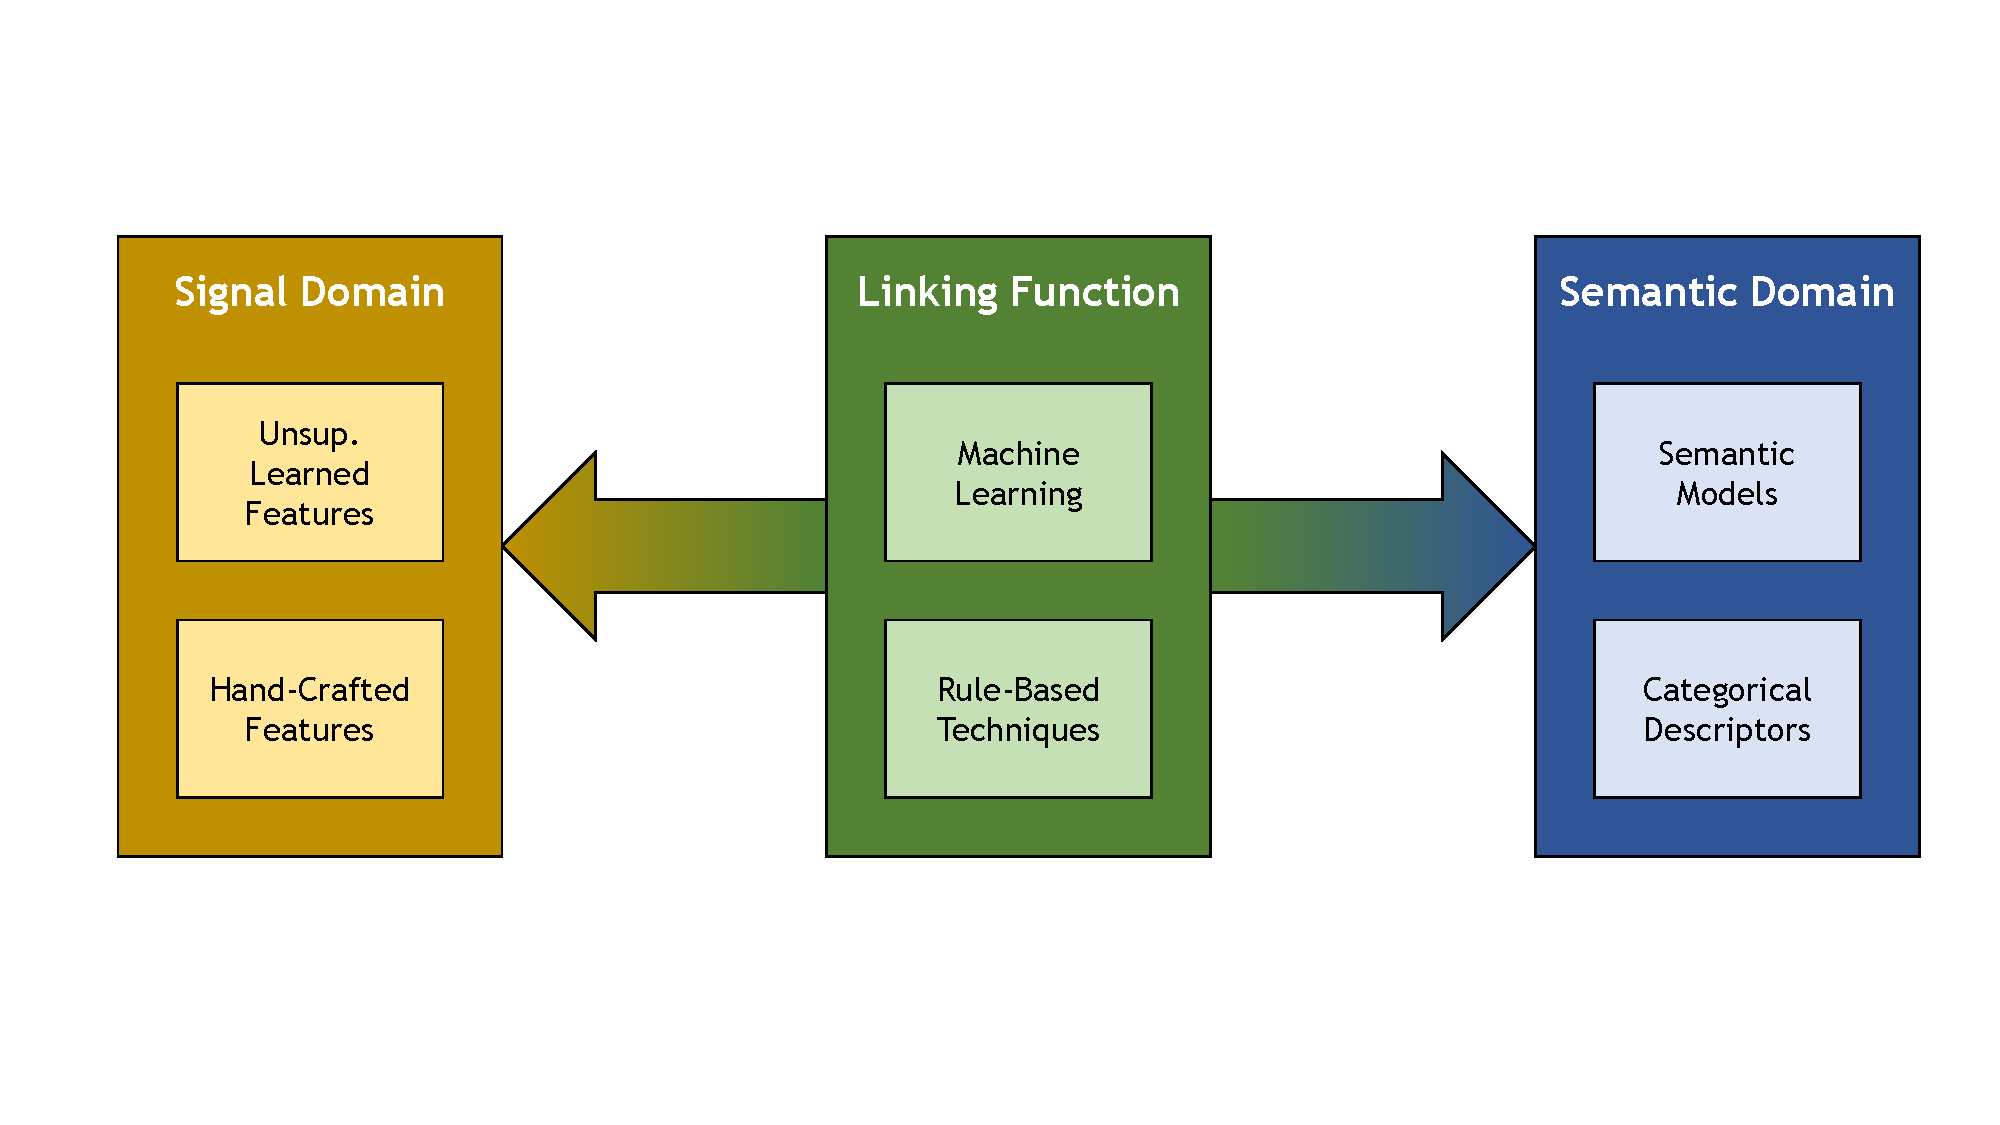
\includegraphics[trim=1.9cm 4.5cm 1.3cm 3.7cm,clip=true,width=\textwidth]{img/intro/schema_new_colorz}
		%\psfig{file=im/ML/logopm.jpg,width=3.5cm}
	\end{center}
	\caption{A visualization of the schema used throughout the thesis}
	\label{fig:intro:scheme}
\end{figure}

\subsection{Feature representation of the signal domain}
%As far as the signal domain is concerned, MIR community has proposed LLFs, MLFs and, most recently, approach based on deep learning.
The MIR literature has developed several techniques to represent the characteristics of the musical content by means of the automatic extraction of related \textit{features}. Such features are traditionally categorized by their level of abstraction from the underlying signal \cite{Celma2008}. In Chapter \ref{Chap:LLFs} we discuss the formalization of the features for the different levels of abstraction.

The lower level of abstraction is captured by the \textit{Low-Level Features} (LLFs ) \cite{Kim2004}, which extract the characteristics related to the physical nature of the audio signal. Such characteristics include the energy or the noisiness of the sound. The LLFs are extracted using clear mathematical formulations, which makes them easy to compute, highly objective, and therefore a reliable formalization for the signal domain. 

On a higher level of abstraction, there are the \textit{Mid-Level Features} (MLFs) \cite{Fu2011}, which concern the aspects of music composition and execution \cite{Muller2011}. While several models have been proposed by the MIR community, there is not a clear formulation to extract MLFs, and they are, in fact, less objective than the LLFs. 

LLFs and MLFs have been manually designed, based on signal processing techniques and studies on human perception and psychology of music. Therefore, they are named \textit{hand-crafted} or \textit{model-based} features and their interpretation is a valuable resource to infer some insight on the signal domain. In order to do so, it is important to deeply understand which aspect is captured by each feature. 

In order to develop such understanding, in Section \ref{sec:NMP} we conduct a feature-based analysis of the Networked Music Performance (NMP) task, where two or more musicians are willing to interact from different locations, by means of an Internet connection \cite{barbosa2003displaced}. Traditional literature on NMP focus on which network architecture can be used to minimize the network delay \cite{saputra2012design,gu2005network,renwick2012sourcenode}. Instead, we investigate which properties of the musical performance, and therefore which features extracted from the signal domain, affect the overall quality performance.  

In some situations, however, the definition of the signal domain is fuzzy and it is not clear which properties are more effective to characterize the domain or which feature can actually capture them. It is not possible, therefore, to address the problems related to such situations using feature-based analysis techniques. In the latest years, a novel and powerful method for feature extraction has emerged, named \textit{deep learning}, that mimic the behavior of the human brain by organizing the information in multiple hierarchical layers \cite{Haykin1998,Goodfellow2016}. Each layer provides a description of the content with different levels of abstraction.% and therefore the deep learning techniques can be used to automatically learn a feature representation of the signal domain.

One of the most interesting properties of deep learning techniques is their ability to learn the feature representation with no specific information on the aspects that need to be extracted, i.e., in an unsupervised manner. While such \textit{unsupervised learned features} have no direct interpretation, they have been proven to be more effective than the traditional hand-crafted and model-based features in several MIR tasks \cite{Hamel2010, Schmidt2011, Humphrey2013}. In Section \ref{sec:LLFs:learned} we offer an overview of the state of the art of deep learning techniques in MIR.

\subsection{Techniques to design the linking function}
%As far as the linking function is concerned, MIR community has proposed to rule-based and machine-learning techniques.

With respect to the linking function, we can use different techniques from the MIR literature, depending on the complexity of the formalization and on how wide the gap between the signal and the semantic domain is. In Chapter \ref{Chap:ML} we discuss the two main approaches for the design of the linking function: rule-based and machine learning techniques. The former strategies are manually designed and developed by researchers and therefore can be used in a limited number of cases. Rule-based techniques are commonly used when the domains are formalized well enough and there is a proper knowledge on the nature of the linking function. 

In most cases, however, the formalization of the domains is not so precise, and the semantic gap is wide, in particular when bridging the gap involves the modeling of the human perception, which is two-fold. On one side, the modeling, concerns the low-level processing of the sensory input, which is affected by the physical sound, and on the other side it involves the processing and high-level interpretation of such input \cite{Bernstein2010}. For this reason, modeling the human perception affects both the signal and the semantic domains, as well as the linking between the two. In such cases, we can use machine learning techniques, which are able to automatically learn a predictive model that links input and output domains. Machine learning techniques have been widely used in MIR tasks \cite{coviello2011,sturm2014}. In Section \ref{sec:ML:models} we provide an overview of some machine learning techniques from two traditional categories: classifiers and regressors \cite{friedman2001}. The former predict an outcome from a set of discrete values, while the latter predict an outcome within a continuous range of values. 


\subsection{Formalization of the semantic domain}
%As far as the semantic domain is concerned, MIR community has proposed classification approaches, categorical approaches, dimensional models and even ontologies.

With respect to the semantic domain, in Chapter \ref{Chap:HLFs} we discuss the so-called \textit{High-Level Features} (HLFs) \cite{Le2013} used for music description. The HLFs provide a formalization of the semantic aspects of music, such as the mood perceived in a song or its genre. However, due to their abstract nature, there is no objective mathematical formulation that we can use for extracting them.
For this reason, it is common to first formalize the semantic domain, and then to design the linking function to extract the semantic description from the musical content or retrieve the musical content from the semantic description.

There are two main approaches to the formalization of the semantic domain: the \textit{categorical} and the \textit{dimensional} \cite{Sordo2012}. The \textit{categorical} approach provides a qualitative description of music, i.e., specifies whether or not a certain feature can be used to describe a song (e.g., \textit{this song is groovy} or \textit{not groovy}). Following the categorical approach, we discuss two different types of formalizations. The former involves the definition of a set of disjoint categories for the description of the songs, while the latter allows the semantics of the descriptors to overlap, i.e., to represent a song with numerous descriptors.

The \textit{dimensional} approach provides a quantitative description, i.e., specifies the degree of descriptiveness of a feature for a song (e.g., \textit{this song is rather groovy}, which might be represented as a value of 0.7 of grooviness). While the categorical approach is easier to use, the dimensional approach supports the possibility to use a nuanced description that is more accurate and closer to the natural language. Because of this more accurate description, the dimensional approach can be used to provide a better formalization of the semantic domain and to define a \textit{semantic model}. 

In Section \ref{sec:HLFs:VA} we review a psychological model for the emotional-related descriptors, the Valence-Arosaul (VA) model \cite{Russell1980}, which involves two dimensional descriptors: \textit{Valence} describes the degree of positiveness (or negativeness) of the mood; and \textit{Arousal} is related to its degree of activation. The Valence and Arousal are in fact two high-level dimensional descriptors, which have been widely used to build a semantic model for the semantic description of the mood conveyed by music \cite{Kim2010,Weninger2014, aljanaki2015emotion}. Since such semantic model closely follows the principles of the psychological VA model, it is commonly named VA model itself. In the VA model, the emotional-related HLFs and the mood conveyed by the music pieces are represented as points in the VA space, where a metric of distance between the points can be defined to model the semantic relation between the objects. 

Given the importance of the VA model, \cite{Bradley1999} presents the ANEW dataset, which is composed of more than 2000 descriptors mapped in the VA space. While the ANEW dataset has been a valuable resource for the MIR community \cite{Kim2010,Weninger2014, aljanaki2015emotion,Yang2012, Cowie2012, Scherer2004} the dataset presents some issues, due to the fact that it is a generic dataset, and it is not tailored for music description. As an example, the distance between two descriptors in the VA space might not be effective to capture their semantic relation for music description. In order to overcome such issues, in Section \ref{sec:HLFs:ANEW} we conduct a research activity aiming at designing a novel space, drawn from the ANEW dataset, where the terms are better conceptually organized for music description. We conduct our research by shaping the novel space according to prior information on how users think of emotional-related descriptors.



% in the music context, and shaping a high-dimensional space built from the ANEW dataset accordingly to the collected information. %This processing helps us to de-clutter the dataset and to find a space where terms follows a better conceptual organization with regard to the music description.


%Second part: overview of the application scenarios
\section{Overview of the application scenarios}
The second part of this work is devoted to apply the aforementioned techniques in a number of real-world scenarios for different MIR tasks.
We gradually increase the complexity of the scenarios, i.e., the complexity of the formalization of signal and semantic domains, and of the definition of the linking function.
In Table \ref{tab:intro:chapters} we list the various application scenarios with the issues to be addressed for each of them. 

\begin{table}[tbp]
\centering
\caption{Structure of the thesis}
\label{tab:intro:chapters}
  \bgroup
  \def\arraystretch{1.5}
\begin{tabular}{||l|>{\RaggedRight}p{2.2cm} |>{\RaggedRight}p{3cm} >{\RaggedRight}p{3cm} >{\RaggedRight}p{2.8cm}||}
\hline
\hline
\textbf{Chapter}  &\textbf{Application}& \textbf{Signal domain} & \textbf{Linking Function} & \textbf{Semantic Domain} \\
\hline
\hline
Chap. \ref{Chap:MSA} & Music \newline Structure Analysis & Poorly known: learned features & Rule-based \newline techniques &  Well known \\
\hline
Chap. \ref{Chap:Bootleg} & Bootleg \newline Detection &  Poorly known: learned features    &  Machine Learning techniques  & Defined but \newline unkown \\
\hline
Chap. \ref{Chap:Violin} & Timbral \newline description of violins & Unknown: learned features    & Machine Learning techniques  & Fuzzy: \newline semantic model \\
\hline
Chap. \ref{Chap:DCSM} & Semantic model for description and retrieval & Musical content  & Information \newline Retrieval system  &  Ambiguous: \newline semantic model\\
%\hline
%Chapter 11 & Multimodal & Unkown & Highly vast \\
\hline
\hline
\end{tabular}
\egroup
\end{table}

%Our work involves the development of music virtual mediators as a linking function between the music physical domain and the user semantic codomain. Depending on the use-case in analysis, the linking function, the domain or the codomain might be hard to be understood, formalized and modeled. For same tasks, the domain and codomain are well defined and they can be easily linked with manual analysis. For some other tasks, the semantic codomain is well defined and easily modeled while there is little on no insight on the best representation for the music codomain. The original contribution of our work follows a gradual approach, that starts with easy scenarios and gradually increases complexity in the application. The main contributes of this thesis are collected in  \cref{Chap:NMP,Chap:MSA,Chap:Bootleg,Chap:ANEW,Chap:Violin,Chap:DCSM}.
%
%
\subsection{Structural boundary detection using unsupervised learned features}
In the first application scenario, we aim at dividing a song into its main structural components, named \textit{sections}, that are commonly used in the western popular music, such as \textit{intro}, \textit{verse}, \textit{chorus} \cite{muller2007towards,muller2015fundamentals}. Since some sections often repeat during the song, e.g., the \textit{chorus}, or some sections can be similar to others, e.g., the \textit{intro} and the \textit{outro}, the knowledge of the \textit{structure} of a song provides a useful insight to tackle the music analysis. Moreover, the knowledge of the structure can also enrich the musical content for retrieval purposes, e.g., by allowing the users to scrape not only among songs, but also within the songs.

The musical structure is traditionally considered as a mid-level feature of music, since it involves the use of prior musicological knowledge. However, the structure of a song also involves cultural aspects of the listeners and a certain degree of subjectivity is often observed during the annotation step \cite{ullrich2014boundary}. For this reason, we will consider the musical structure as a feature in between the middle and the high level of abstractness. 

Due to the vast musicological literature on Music Structure Analysis (MSA), the musical structure, which represents the semantic domain, is well formalized and the MIR community has identified some principles and developed the relating algorithms to model the linking function. However, it is not clear which aspects of the musical content are involved in MSA and therefore which features are more effective to represent the signal domain.

In Chapter \ref{Chap:MSA} we address the issues related to the formalization of the signal domain by using deep learning techniques to extract unsupervised learned features. We use the learned features with rule-based techniques developed within the MIR community to extract the structure of the songs. We compare the performance achieved with learned features with those achieved using hand-crafted features. The comparison highlights the improvement achieved using the deep learning techniques for the signal domain formalization.

\subsection{Bootleg detection using unsupervised learned features}
The wide diffusion of portable media devices has led to a considerable increase of user-generated content, including malicious and tampered content \cite{Melloni2015}. In this regard, one of the main phenomena in music is represented by the production and diffusion of bootlegs. A bootleg is a unofficial recording of a live performance that is edited and shared as official \cite{Bestagini2013b}. In Chapter \ref{Chap:Bootleg} we address the problem of the automatic detection of bootlegs, by classifying a song into three categories: official live recording, official studio recording or bootleg. Such automatic categorization is not only useful for forensic purposes, but also for high-level description.

The semantic domain of the task is rather easy to formalize, due to the limited number of categories with which we intend to represent the songs. The signal domain is instead poorly known, since it is hard to deduce which aspects from the different categories characterize the songs and therefore which features are more discriminative for the task. Furthermore, with respect to the previous scenario, in this scenario we do not have any prior knowledge on the linking function between the two domains, and in fact the editing of bootlegs can make the task challenging even for a human listener.

We use unsupervised deep learning techniques to extract a salient representation of the signal domain, and we employ classification machine learning techniques to model the linking function. By applying this setup to the bootleg detection task, we achieve significant results, especially when compared with the same setup with hand-crafted features.


\subsection{Automatic description of the timbre of violin using unsupervised learned features}
One of the main MIR tasks is the automatic annotation of music pieces, i.e., the extraction of the high-level features from a feature representation of the musical content \cite{brossier2006}. Music concerns many different high-level aspects, such as the mood, the genre or the timbre. The description of each of these aspects involves the use of a large number of HLFs. In Chapter \ref{Chap:Violin} we focus on a specific scenario of automatic annotation of the timbre of violins.  %entire songs, instead of single instruments.

In this case the semantic domain is hard to be modeled, since there are numerous descriptors for the timbre of the violins, whose semantics is fuzzy and often relies on metaphors and synaesthesia, i.e., the use of descriptors from a a different sensory perception field, such as \textit{warm} or \textit{cold} \cite{Zanoni2014}.  %with poor formalization on their semantics. 

The characteristics involved from the signal domain are also unknown, since we can make little assumptions on which features are more likely to describe the timbre qualities. Moreover, we have no knowledge on the kind of linking function we need to design, since we must emulate the human perception and therefore a rule-based algorithm is unlikely to be effective. This scenario is extremely challenging and, in fact, only trained users such as musicians, teachers or violin makers are capable of providing a reliable description of the timbre.

%While some descriptors are used to describe general characteristics of a song, other describe more specific qualities of single instruments or parts. As an examples, music teachers and students, musicians, composers, directors and instrument makers share a common dictionary to describe the timbre of the instruments, i.e., some inner characteristic of the sound of an instrument or of an execution. The semantics of such descriptors has not a proper definition and often relies on metaphors and synaesthesia, i.e., the use of descriptors from a a different sensory perception field, such as a \textit{warm} or \textit{cold} sound \cite{Zanoni2014}. In this scenario we work on the definition of a dimensional semantic model for the specific case of the description of the sound quality of violins. We aim at design an approach for the automatic description of the timbre of violin recordings within the defined semantic model. 

We formalize the semantic domain by designing a dimensional semantic model, where the HLFs are identified by bipolar descriptors, i.e., a term and its antonym. %The dimensionality of the model allows the system to describe a timbre as a vector in the quality-dimensional space, and finds an affordable solution for the formalization of the semantic domain. 

Regarding the signal domain, we use unsupervised learned features, which allows us to tackle the complexity of feature design and selection. Finally, we employ several machine learning techniques to bridge the semantic gap and to design the linking function as a regression model. The semantic model provides a useful tool to describe the timbre of a violin as a graded linear combination of its main descriptors, and we can subsequently expand the resulting solution to more generic application scenarios, such as the annotation of other high-level aspects of music pieces.

\subsection{A Dimensional Contextual Semantic Model for music description}
The main task of our work is to develop an automatic system that allows the users to semantically retrieve  musical content. However, when people describe music with natural language, they use terms that are both evocative and ambiguous, and could have several possible meanings (\textit{polysemy}) \cite{lee1999}. It is not rare indeed that a single term describes several high-level aspects of the music, such as the term \textit{calm}, that can describe both the mood conveyed by a song or its dynamics. In Chapter \ref{Chap:DCSM} we investigate a semantic model capable of taking the fuzziness and ambiguity of natural language into account, to be included in a semantic retrieval system. 

This task requires the definition of a semantic model that involves different high-level aspects (\textit{contexts}) of music and possibly taking into account the ambiguity issues such as polysemy. 
In this scenario, the linking function follows the opposite direction with respect to the previous ones, since it is used to retrieve the musical content, which we assume to be already formalized with a high-level description.

We address the polysemy issues by including several descriptors from different contexts in a unique dimensional contextual semantic model (DCSM). In the DCSM, the HLFs are allowed to belong to different contexts and the semantic relation between them is defined for each of the context to which they belong. We embed the DCSM in a system that allows users to retrieve the musical content by means of natural language queries.

\section{List of Publications}
The publications relative to the work presented in the thesis are listed in the following.


\textbf{Peer-reviewed journal papers:}
\begin{itemize}
\item Cristina Emma Margherita Rottondi, Michele Buccoli, Massimiliano Zanoni, Dario Garao, Giacomo Verticale, Augusto Sarti, \textit{Feature-Based Analysis of the Effects of Packet Delay on Networked Musical Interactions}, in Journal of the Audio Engineering Society 63 (11), 864-875, November 2015.	
\end{itemize}

\textbf{Peer-reviewed conference proceedings:}
\begin{itemize}
\item Michele Buccoli; Davide Andreoletti; Massimiliano Zanoni; Augusto Sarti; Stefano Tubaro, \textit{Unsupervised feature learning for Music Structural Analysis}, in Proceedings of 24th European Signal Processing Conference (EUSIPCO), Budapest, Hungary, August 2016;
\item Michele Buccoli, Massimiliano Zanoni, Gy\"orgy Fazekas, Augusto Sarti, Mark Sandler and Stefano Tubaro, \textit{A higher-dimensional expansion of affective norms for English terms for music tagging}, in Proceedings of 17th International Society for Music Information Retrieval Conference (ISMIR), New York City, USA, August 2016;
\item Michele Buccoli, Massimiliano Zanoni, Francesco Setragno, Augusto Sarti, Fabio Antonacci, \textit{An Unsupervised Approach To The Semantic Description Of The Sound Quality Of Violins}, in Proceedings of 23rd European Signal Processing Conference (EUSIPCO), Nice, France, August 2015;
\item Michele Buccoli, Alessandro Gallo, Massimiliano Zanoni, Augusto Sarti, Stefano Tubaro, \textit{A Dimensional Contextual Semantic Model For Music Description And Retrieval}, in Proceedings of IEEE International Conference on Acoustics, Speech and Signal Processing (ICASSP), Brisbane, Australia, 2015;
\item Michele Buccoli, Paolo Bestagini, Massimiliano Zanoni, Augusto Sarti, Stefano Tubaro, \textit{Unsupervised Feature Learning For Bootleg Detection Using Deep Learning Architectures}, in Proceedings of IEEE International Workshop on Information Forensics and Security (WIFS), Atlanta, USA, December 2014

%A Music Search Engine Based Of Semantic Text-query Query
%Michele Buccoli, Massimiliano Zanoni, Augusto Sarti, Stefano Tubaro
%in Proceedings of the 15th international workshop on multimedia signal processing - MMSP 2013 - September 30 - October 02, 2013, Pula (Sardinia), Italy
\end{itemize}

\textbf{Workshop presentations:}
\begin{itemize}
\item Michele Buccoli, Alessandro Gallo, Massimiliano Zanoni, Augusto Sarti, Stefano Tubaro, \textit{A Dimensional Contextual Semantic Model For Music Description And Retrieval}, in DMRN+10: Digital Music Research Network One-day Workshop 2015, London, UK, 2015.
\end{itemize}



%\TBD{
%Journal submissions in preparation:}
%\begin{itemize}
%
%\item Michele Buccoli, Massimiliano Zanoni, Augusto Sarti, Fabio Antonacci, \textit{A work on wholodance}, in IEEE Trans somewhere;
%\item Michele Buccoli, Massimiliano Zanoni, Augusto Sarti, Fabio Antonacci, \textit{A work on customized music similarity}, in IEEE Trans somewhere;
%\item Michele Buccoli, Massimiliano Zanoni, Augusto Sarti, Fabio Antonacci, \textit{A work on mood segmentation}, in IEEE Trans somewhere.
%\end{itemize}
%






 % uncomment if you want part I
\part{Definition and formalization of the components of the schema}
% !TeX spellcheck = en_US
\chapter{Feature representation of the signal domain}
\label{Chap:LLFs}
In order to develop systems that allow the users to access large music libraries, it is crucial to define and formalize the problem from the perspective of the content, i.e., the signal domain. The signal domain involves three main levels of information: the physical level, which is related to the origin and propagation of the audio wave and can be analyzed with signal processing techniques; the physiological perceptual level, which concerns how the sound is perceived by the auditory system; and the musical level that describes musicological aspects. In this Chapter we  present an overview of the state of the art needed to formalize the audio signal domain.

The MIR community developed and designed several techniques to describe the signal domain by automatically extracting features from the audio signal. Such features describe different aspects of the sound at various levels of abstraction, from those related to the energy, the spectrum or the timbre, to those regarding musical aspects of the music performance. A description of all the features employed in Music Information Retrieval is beyond the scope of this work, and in the following Sections we discuss the most popular features and those that we use throughout the thesis.

In Section \ref{sec:LLFs:hand-crafted}, we describe the so-called \textit{hand-crafted} and \textit{model-based} features, that are manually designed by scientists by means of exact mathematical formulations or of perceptual/musicological models, respectively. These features are usually divided into low-level features, that capture a specific characteristics of the audio signal by means of the exact mathematical formulations, and mid-level features that make use of the musicological aspects of the songs. For the sake of brevity, in the following discussion we will refer to both kind of features as hand-crafted features, since the perceptual or musicological models of the model-based features have been manually designed as well. 

In order to better explore the potential of such features, in Section \ref{sec:NMP} we present our research activity on Networked Music Performance, where the design of a network architecture benefits from a feature-based analysis of the (music) signal domain of the problem. In this study, we make use of both spectral low-level features captured from the audio signal and rhythmic mid-level features extracted from the scores of the corresponding musical pieces. This study was published in the Journal of Audio Engineering Society \cite{Rottondi2015}.

Finally, in Section \ref{sec:LLFs:learned}, we describe the so-called \textit{learned} features, which are automatically extracted by means of deep learning techniques, and we focus on the deep architecture we used in our works. %We also present a brief overview of deep learning techniques from the state of the art that have been used to extract a representation of the music signals.


\section{Hand-Crafted and Model-Based Features}\label{sec:LLFs:hand-crafted}
When analyzing a problem, it is important to understand which aspects are more useful to characterize the domain of the problem. It is therefore crucial to understand the insight we can infer from the various features and hence which are the most suitable ones to capture the different aforementioned aspects. The hand-crafted and model-based features provide a formalization of the problem related to the musical content, by providing a reliable description of the audio signal and of the underlying musical aspects. Such a low-level representation is a valuable resource for  researchers, scientists and musicians, who can interpret the underlying information.  

Due to the strong relevance of hand-crafted features in Music Information Retrieval, several tools have been developed to automatically extract them, such as the MIRToolbox for Matlab \cite{Lartillot2007}, LibRosa for Python  \cite{brian_mcfee_2015_18369}, Marsyas \cite{tzanetakis2000marsyas} and Essentia\cite{bogdanov2013essentia} for C++ and Sonic Annotator as a command line routine combined with the VAMP plugins \cite{chris2010a}. 

The hand-crafted features are traditionally classified as Low-Level and Mid-Level Features \cite{Celma2006,Zanoni2013Thesis}.

Low-Level Features (LLFs) are directly extracted from the audio signal by means of an exact mathematical formulation. LLFs include descriptors extracted from the time-domain representation of the audio signal, such as the Zero Crossing Rate (ZCR), or from the frequency-domain representation --often, the short time Fourier Transform (STFT). Since the human auditory system mainly focus on the 
frequency content of sounds, the features extracted from the spectrum, also referred to as \textit{spectral features}, or \textit{spectral descriptors}, are more frequently used. 

Spectral features are important to capture properties of the spectrum from which we can infer the perceptual qualities of the sound. We can however reverse the approach by designing features that measure and return a signal from the perceptual representation of the sound. We can do so by exploiting the information on how the human auditory system works. From the studies on psychoacoustics, we know that the human perception of frequency is logarithmic, as well as the perception of loudness. In particular, the decomposition of a sound in the correspondent frequency components is performed within the spiral-shaped cavity named \textit{cochlea} in the inner ear. The cochlea acts as a filter bank for different ranges of frequencies \cite{miotto2011}. 

The \textit{Mel-Frequency Cepstral Coefficients} (MFCCs) are a set of low-level features that exploit a model from psychoacoustics on the human auditory system to provide perceptual cepstral features. The MFCCs have become one of the most widely used descriptors for Music Information Retrieval \cite{muller2007information, muller2015fundamentals}. Due to their ability to provide a compact representation of the distribution of the energy values of the spectrum, they have also been widely employed to capture properties of the timbre and therefore they are also referred to as \textit{timbral descriptors}. 

The Low-Level Features are commonly computed over a frame representation of the audio signal, with typical values of the frame length being 1024 or 2048 samples, i.e., around 50-100 ms for a 44.1 kHz sampling frequency. This leads to a tremendous amount of data for the music representation, which often results in memory overload and computational issues. A typical approach to create a more compact representation is to \textit{pool} together several frames to compose a larger analysis window. This approach makes the features less accurate and precise in the time domain, but it may also increase the quality of the captured features by smoothing possible outliers. The commonly used pooling technique is based on the average of the feature values over frames within fixed-length analysis windows \cite{Bestagini2013,zanoni2015training}. 

LLFs are designed and employed to extract a high number of properties of the signal domain. The musical content can be further analyzed from the perspective of the signal by considering not only the time-domain or frequency-domain representation, but also their interpretation in light of the musicological field.

The Mid-Level Features (MLFs) provide a higher level of abstraction from the audio signal by including some musical knowledge into the feature extraction process. Various approaches have been proposed to extract musically meaningful features, using both model-based approaches and machine learning techniques. Several of the issues related to the Mid-Level Features are still open and the MIREX competition holds every year to compare the performance of approaches proposed by several research groups within the MIR community \cite{downie2014ten}.

The MLFs are either directly extracted from the audio signal or estimated from an intermediate symbolic representation of the songs where the components from the sheet music are structured and explicit. There is a lower availability of symbolic representation of music pieces, since it requires a manual effort to be exactly annotated. Nevertheless, when available, such a representation 
is more reliable for the analysis of complex or abstract information, like the harmonic or rhythmic complexity, the degree of surprise or the difficulty in listening. In this regard, some tools for the automatic extraction of features from symbolic notation have been developed, such as the MIDI Toolbox \cite{Eerola2004}.

Two of the main broad aspects that can be described as MLFs are the harmony and the rhythm. The former is composed of the pitch of notes, chords, keys and the modes, the latter extracts beats and bars, and the rhythmic patterns from the music pieces \cite{muller2007information,muller2015fundamentals,bello2010identifying,Nieto2D}. With respect to the harmony of a music piece, one of the most widely used \textit{tonal descriptor} is designed to capture the pitches of which the harmony is composed. The \textit{chromagram} captures the distribution over time of the different pitches, regardless to the original octave, by exploiting the prior information on the frequency corresponding to the different pitches in the equal-tempered scale \cite{weihs2016music}. Regarding the rhythm, the \textit{tempo} is a useful \textit{rhythmic descriptor} that is often used to assess the speed of execution of a given piece. Other rhythmic descriptors we use in our thesis include the \textit{Event Density} and the \textit{Rhythmic Complexity}, that are computed from a symbolic representation of the music piece and estimate the average density of notes and the difficulty to execute a given piece, respectively \cite{Eerola2004}.

The musicological properties captured by MLFs are also a helpful resource for the design of other algorithms. As an example, with regard to the aforementioned pooling techniques, rhythmic descriptors can be used to pool together the frames that occur between two consecutive beats. This \textit{beat-synchronized} representation is independent on the variation of tempo and hence has been proved to be particularly useful for cover identification and structure analysis tasks \cite{Ellis2007,Nieto2D}.

Several LLFs and MLFs have been proposed in the literature, depending on the task under analysis and therefore on the involved properties from the audio signal. A partial overview of LLFs and MLFs is provided in  \cite{mckinney2003features,Kim2005,weihs2016music}. However, the amount of works involving LLFs and MLFS is huge and we will here just mention some of them, as a demonstration of their extremely high flexibility for a number of different tasks.

The LLFs and MLFs have been widely used to compute a representation of the signal domain for the task of automatic annotation, as in \cite{eck2008automatic} where a set of spectral features are used, in \cite{barrington2008auto} with MFCCs. Features from different levels can be combined together to obtain a multi-level representation: for examples, mid-level rhythmic features are combined with low-level timbral features in \cite{orio2013combining}; and with low-level spectral descriptors and high-level lyric-based descriptors in \cite{neumayer2007integration}. Mood Emotion Recognition (MER) is a subfield of MIR that focuses on the annotations of music with emotional-related descriptors and it has been addressed in several works. Features used in MER include spectral, timbral, and tonal descriptors \cite{schmidt2010prediction, xianyu2016svr, deng2015dynamic, chen2014linear}, while a more detailed review is proposed in \cite{Barthet2012}. The description provided by LLFs has also been used to compare two audio recordings by defining a similarity function between their feature-based representations \cite{pampalk2005improvements}. This approach is used in \cite{Kim2004} to perform audio classification with a query-by-example: an audio recording is presented to a system, which retrieves the acoustically-similar recordings in a dataset. Low-Level and Mid-Level Features, often MFCCs and chromagram, are also widely employed for the analysis of the music structure as a frame-level description of a song \cite{levy2008structural,ong2005semantic,kaiser2012music}. A possible interpretation of some LLFs can be inferred by correlating them with high-level descriptors and analyzing the correlation values, as it is done in \cite{Zanoni2014} for the sound quality of violins.


% % DESCRIZIONE FEATURES
In Table \ref{tab:LLFs:features} we list the features that are employed in this work and especially in the study in Section \ref{sec:NMP}. A more extensive discussion of the features used in this work is provided in the Appendix \ref{app:LLFs}. 





\begin{table}[!tb]
	
	\vspace{1cm}
	\caption{Low-Level and Mid-Level Features employed in this work}
	\centering %\small
	\label{tab:LLFs:features}
	\bgroup
	\def\arraystretch{1.5}
	\begin{tabular}{||l|p{1.9cm}|p{1.8cm}|l|p{6cm}||}
		\hline
		\hline
		Level & Name & Type & Symbol & Interpretation \\
		\hline
		\hline
		LLFs & Spectral Centroid & Spectral Descriptor & $SC$ & "Center of mass" of the distribution of the energy values of the spectrum. It is related to the "brightness" of the sound. \\
		\hline
		LLFs & Spectral Spread & Spectral Descriptor & $SSp$ & Standard Deviation of the aforementioned distribution (spectral distribution). It is related to the noisiness of the sound. \\
		\hline
		LLFs & Spectral Skewness & Spectral Descriptor & $SSk$ & Symmetry of the distribution around the spectrum\\		
		\hline
		LLFs & Spectral Kurtosis & Spectral Descriptor & $SK$ & Resemblance of the spectral shape with a Gaussian bell curve. \\
		\hline
		LLFs & Spectral \newline Entropy & Spectral Descriptor & $SE$ & Entropy of the spectrum distribution. It is related to the noisiness of the sound. \\
		\hline
		LLFs & Spectral Flatness & Spectral Descriptor & $SF$ & Degree of flatness of the shape of the spectrum. It is related to the noisiness of the sound. \\
		\hline
		LLFs & Mel-Frequency Cepstral Coefficients & Timbral Descriptors & $MFCC$ & Compact timbral descriptors from psychoacoustic model of the human auditory system. \\
		\hline
		MLFs & Chroma & Tonal Descriptors & --- & Histogram of the pitch classes, regardless to the octave. \\
		\hline
		MLFs & Tempo & Rhythmic Descriptor & --- & Speed of execution of a piece. \\		
		\hline
		MLFs & Event \newline Density & Rhythmic Descriptor & $ED$ & Average number of onset events per second. \\
		\hline
		MLFs & Rhythmic Complexity & Rhythmic Descriptor & $RC$ & Weighted sum of different metrics of the onset. It estimates the rhythmic complexity of a given piece \\		
		\hline
		\hline
	\end{tabular}
	\egroup
	\vspace{1cm}
\end{table}


\vspace{3cm}
\section{A feature-based analysis scenario: Networked Music Performance}
\label{sec:NMP}
 
The feature-based representation of the signal domain is not only useful for the linking with the semantic domain, but also for addressing those problems that do not involve the high-level meaning of the music. Such problems, indeed, can highly benefit from a preliminary analysis of the signal domain by means of the manual interpretation of its feature-based representation. In order to use such features, it is required to hold a full knowledge of the characteristics they are able to extract. In this Section, we discuss a research activity to develop a better understanding of the features and to demonstrate their use for a manual analysis for the task of Networked Music Performance. The Networked Music Performance (NMP) systems aspire to revolutionize interactive music performances (e.g. remote rehearsals, music teaching) by allowing remote players to interact with each other from remote physical locations through an Internet connection. 

One  of the known limiting factors of distributed networked performances is the impact of the unavoidable packet delay and jitter introduced by IP networks, which make it difficult to keep a stable tempo during the performance. Computer-network systems enabling music performance have been investigated starting from the \lq 70s \cite{barbosa2003displaced} and recently different network architectures have been proposed as enabling design paradigms for NMP systems, ranging from client-server \cite{saputra2012design,gu2005network} and master-slave \cite{renwick2012sourcenode} to decentralized peer-to-peer infrastructures \cite{stais2013networked,chafe2011living}. 

%The delay tolerance is typically estimated to be 20-30 ms \cite{carot2009fundamentals} (corresponding to the time that the sound field takes to cover a distance of 8-9 m), which has been shown to correspond to the maximum physical separation beyond which keeping a common tempo for rhythmic music interaction without conductor becomes difficult. However, the sensitivity to delay and the quality of the musical experience in the context of NMP is influenced by several additional factors \cite{Bouillot2007}. In \cite{barbosa2011influence}, the authors investigate the correlation between perceptual attack times of the instrument (i.e., the time that the instrument takes to reach its maximum loudness) and the sensitivity to network delay, concluding that instruments with a slow attack (e.g. strings) usually tolerate higher latency. In \cite{Chew2004}, the authors investigate the correlation between accepted network latency and the genres of pattern-based music. 

Other limiting factors of NMP depend on the performance itself, including the qualities of the music instruments that are played during the performance and the qualities of the music that is performed. In \cite{barbosa2011influence}, two classes of instruments are defined, with slow or fast attack times, and it is found that the use of instruments with a slow response helps the musicians to be less sensible to the latency issues. In \cite{Chew2004} some broad class of music genres are defined to investigate their correlation with the tolerance to the network latency. The above-mentioned studies conduct a qualitative analysis of the additional factors to investigate their correlation with the sensitivity to delay and the overall quality of the music performance. This qualitative analysis, however, does not provide information on the degree of the impact of the various factors to the final tolerance to the delay. A quantitative analysis, instead, can be more useful to better understand the issues raised by NMP and to potentially relax the latency constraints for the design of the network architecture. 

In this Section, we aim at conducting a quantitative study about the effects of some acoustic properties on the musicians' tolerance to the delay and on the quality of music performance. We perform the quantitative study by taking advantage of the dimensional representation of the features \cite{Kim2005,Zanoni2012}. We are interested in the objective qualities of the musical content, therefore the signal domain is represented by means of a set of low-level and mid-level features. We analyze the NMPs by means of quality metrics, for which we extract the trend of the tempo kept during the performance and we collect annotations from the musicians about the perceptual quality of the musical interaction. We then investigate the quantitative correlation between the feature representation of the signal domain and the quality of performances by manually analyzing the resulting data. This research activity allows us to develop a better understanding of the low-level and mid-level features by investigating which factors affect the subjective and objective quality of a NMP. As a result of the activity, we are able to estimate which network constraints must be satisfied depending on the different properties of the music that will be performed.

In the following we provide an overview of the state of the art and theoretical background on NMP (Section \ref{sec:NMP:background}). In order to conduct this analysis, we implemented a testbed for psycho-acoustic analysis emulating the behavior of a real IP network in terms of variable transmission delay and jitter, and we recorded a set of NMPs with different musicians, instruments, songs and tempi within the song. We present the details on the setup of the testbed in Section \ref{sec:NMP:testbed}. The obtained recordings are processed in order to extract the features for the signal domain and the quality metrics of the performances. We describe the extraction techniques in Section 
\ref{sec:NMP:domain}. Finally, in Sections \ref{sec:NMP:qualResults} and \ref{sec:NMP:quantResults} we present the results of the manual analysis of the collected data and we draw some final considerations in Section \ref{sec:NMP:conclusions}.

In our study we conducted a set of experiments with both male and female musicians. In the following discussion, therefore, we use the \textit{singular they} with the gender-neutral meaning. 

%such as the rhythmic complexity of the performed piece, the timbral characteristics of the instruments and the type of musical part that is being performed (e.g. melody, chord comping, sustained harmony) has not yet been proposed in the literature. 


\subsection{Background}\label{sec:NMP:background}
In order to reproduce realistic environmental conditions for NMP, several technical, psycho-cognitive and musicological issues must be addressed. The musicians in fact are required to perform from different physical locations, which introduce some issues due to the difficulty of playing together with no visual clues available. In \cite{Vera2013,Vera2013b} the authors focused on such cues by investigating the ensemble synchronization under restricted line of sight and they show how the trained musicians are able to rely on non-visual cues such as the breath \cite{Vera2013} or the modulation of the amplitude \cite{Vera2013b}.

At the network level, instead, very strict requirements in terms of latency and jitter must be satisfied to keep the one-way end-to-end transmission delay below a few tens of milliseconds. The overall delay experienced by the players includes multiple contributions due to different stages of the audio signal transmission: the first is the processing delay introduced by the audio acquisition, processing, and packetization; the second is the pure propagation delay over the physical transmission medium; the third is the data processing delay introduced by the intermediate network nodes traversed by the audio data along their path from source to destination, the fourth is the playout buffering which might be required to compensate the effects of jitter in order to provide sufficiently low packet losses to ensure a target audio quality level.

Some preliminary studies on the delay tolerance for live musical interactions have already appeared: in \cite{gurevich2004simulation,chafe2010effect,chafe2004effect,chafe2004network} the authors evaluated the trend of tempo variations (measured in Beats Per Minute - BPM) while performing predefined rhythmic patterns through hand clapping, in different latency conditions. A similar analysis was integrated with an evaluation of the musicians' subjective rating of the performance quality in \cite{carot2009towards}. In \cite{barbosa2011influence}, the authors show that the human auditory system focuses on onsets produced by instruments with a short or almost impulsive attack time, whereas it tends to perceive less immediately those onsets associated to instruments with a slow attack. The impact of delay on the synchronism of the performance is therefore expected to be more clearly perceivable when using musical instruments with a fast attack, rather than when using instruments with a slower attack time. This means that the choice of musical instrument are informative in presence of network delay. In practice, however, musicians tend to adjust their playing technique according to the specific attack time of the instrument played. For example, organ players are used to naturally compensating the delay elapsed between the pressure of the keyboard keys and the sound emission from the pipes, as well as the time that the sound takes to travel back from the pipes to the musician. To a smaller extent this is also true for piano players. In this case the delay between pressing a key and detecting the corresponding note onset varies between $30$ and $100$ ms, depending on sound loudness and musical articulation (e.g. \textit{legato, staccato}) \cite{askenfelt}. For some categories of instruments, it has been shown that the expressive intention and direction of the musician (i.e., subjective artistic and interpretation choices, which are in turn affected by a particular emotional state during the performance) can have a significant impact on sonological parameters such as attack, sustain and decay time \cite{clarinet}. In our study we do not evaluate the impact of the instrument attack time on the performance interplay, and consider this attack time simply as part of the overall delay perceived by the musician. 

One specific aspect that has been addressed in the literature is the role played by a musical instrument in a performance. In western music, some instruments have a more pronounced ``leading'' role than others. In \cite{Carot07networkmusic} the authors define two main musical roles, the \textit{solo} and the \textit{rhythmic} role, and they identify some approaches of musical interaction that depend on the network delay that is set. The best situation is called \textit{Realistic Interaction Approach} (RIA), when the network delay is lower than 25 ms and both roles can play with total interaction as if they were playing in the same physical place. Beyond the 25 ms threshold, the performance usually follows a \textit{Master-Slave Approach} (MSA), where the rhythmic part leads the interaction with the solo part, as the Master of the performance, and the solo part follows the provided tempo, acting as the Slave. The rhythmic players are therefore expected to keep a steady tempo even when the other musicians are playing off-tempo. From the solo perspective, the synchronization is good, while the interaction is more difficult. When the delay approaches the 50 ms value, \cite{Carot07networkmusic} suggests a behavior named \textit{Laid Back Approach} (LBA), whereby the solo plays slightly behind the groove led by the rhythmic part. This approach is a common solo style in jazz music and produces an acceptable interaction for the musicians even for high delay. An alternative MSA approach is the \textit{Delayed Feedback Approach} (DFA), where the rhythmic part holds its leading role, while receiving their own sound feedback with a slight delay. If the delay of the feedback is similar to the network delay, the musician who is playing the rhythmic role will listen to their feedback in sync with the solo part. In DFA, the solo musician perceives a synchronization quality similar to the MSA, while it is more challenging for the rhythmic musician to handle the delayed feedback. 

In our study we extend the set of roles to four, where we split the rhythmic parts into chord comping and drums, and we include the sustained harmony. For this reason, we do not use the taxonomy of approaches defined by \cite{Carot07networkmusic}.



\subsection{Testbed setup}\label{sec:NMP:testbed}
\begin{figure}[!tb]
  \centering
  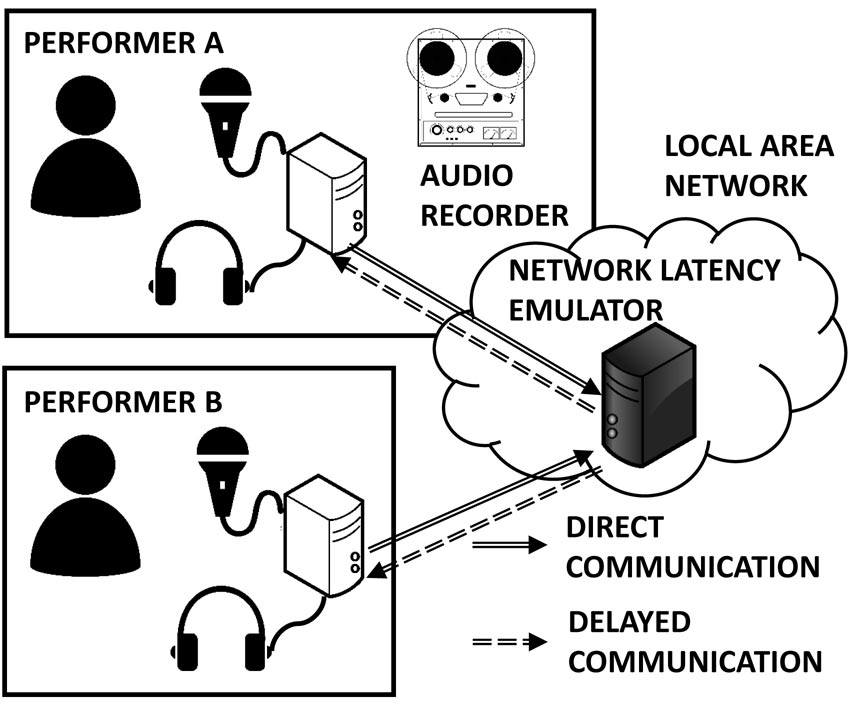
\includegraphics[width=.95\textwidth]{img/NMP/setup}
  \caption{Testbed setup}
 \label{fig:NMP:testbed}
\end{figure}
In order to analyze the correlation of the music played with the tolerance to delay, we implemented a testbed setup to emulate the NMP scenario. Our experiments involved pairs of musicians playing in two phono-insulated near-anechoic rooms (sound rooms), to avoid any audio feedback or visual contact, as depicted in Figure \ref{fig:NMP:testbed}. Visual contact was provided not even by means of video streaming because video processing time is larger than audio processing time and would have increased the minimum achievable end-to-end delay. The musicians were also forbidden to verbally communicate to their counterpart during the performance. Each room was equipped with a desktop PC running the SoundJack software, which is a peer-to-peer publicly available software \cite{carot2008distributed} that also implements a direct real-time evaluation of the experienced one-way end-to-end latency (thus including processing, buffering and playout delays).  Each PC was connected to an external sound card via high-speed connection (FireWire and AES/EBU) operating at a sampling rate of 48 kHz. The sound card was connected to high-quality headphones and microphones. An additional PC (with two network interfaces) running the WANem network emulator \cite{wanem} was placed in between. 
Through the WANem emulator we could manually select the delay and jitter of the emulated network, in order to replicate the NMP real-world scenario. The network interfaces of the three PCs were connected to each other through a Fast Ethernet switch. The PCs of the sound rooms were configured to communicate exclusively through the interfaces of the WANem emulator, thus preventing any direct communication between them. 

Each musician was able to hear their own instrument as well as the instrument of the other player through headphones. The choice of the headphones was made in order to minimize the possible delay and to avoid loop-feedback effects. The two audio signals were transmitted through the Local Area Network of the building. During the experiments, all the involved LAN segments were free of other traffic. The audio tracks were recorded as follows: the audio data generated by \textit{performer A} were recorded directly after the electric transduction of the microphone, whereas the audio data generated by \textit{performer B} were recorded from the SoundJack feedback after propagation of the audio stream through the network, i.e. as heard through \textit{performer A}'s headsets.

%\subsection{Scores and Network Parameters}
We considered three different music pieces: \textit{Yellow Submarine} (by The Beatles) at different values of BPM (88,110,132), \textit{Bolero} (by Maurice Ravel), and \textit{Master Blaster} (by Stevie Wonder), arranged for four different parts: main melody (M), chord comping (CC), sustained harmony (SH), and drums (D).  Scores were released to the musicians in advance.

\begin{table}[tb]
  \caption{Combination of parts played in each experiment session. M: main melody; CC: chord comping; SH: sustained harmony; D: drums}
  \centering %\small
  \label{tab:NMP:sessions}
  \bgroup
  \def\arraystretch{1.5}
 \begin{tabular}{||c|c|c|c|c||}
 \hline
 \hline
  Id & Instrument A& Part A & Instrument B & Part B \\
 \hline
 \hline
  1 & Acoustic Guitar & M & Classic Guitar & CC\\
  2 & Electric Piano & M & Drums & D\\
  3 & Keyboard (strings)  & SH & Drums & D\\
  4 & Keyboard (strings)  & SH & Electric Guitar & CC\\
  5 & Clarinet & M & Clarinet & M\\
  6 & Electric Guitar  & CC & Drums & D\\
  7 & Keyboard (strings)  & SH & Clarinet & M\\
 \hline
 \hline
   \end{tabular}
   \egroup
\end{table}

Our experiments involved 8 musicians with at least 8 years of musical experience, all with semi-professional or professional training level, and 7 instruments, i.e.:
Acoustic, Classic and Electric Guitar, Clarinet, Drums, Electric Piano and Keyboards with strings samples. Each musician played at least one of the instruments. The musicians were grouped in 7 pairs according to the combinations listed in Table \ref{tab:NMP:sessions}. Note that some musicians performed in more than one pair (e.g., one clarinetist performed twice, i.e. in pairs 5 and 7, whereas the pianist played electric piano and keyboard in pairs 2, 3, 4 and 7). For a given pair, each musician performed only one of the four parts for each of the three considered musical pieces, as detailed in Table \ref{tab:NMP:sessions}. Musicians in pairs 5 and 6 had regularly performed together in the last years, where the remaining pairs had never played together before. However, in order to avoid biases due to prior common performances, all the pairs were allowed to practice together in the testbed environment until they felt sufficiently confident. Before participating to our experiments, none of the players had ever experienced networked music interactions.

\begin{table}[tb]
  \caption{Tested network parameters and tempo settings}
  \centering %\small
  \label{tab:NMP:param}  
  \bgroup
  \def\arraystretch{1.5}
  \begin{tabular}{||c|c|c|c||}
\hline
\hline
 Piece & $\delta$ [BPM]& $\mu$ [ms]& $\sigma$ [ms]\\
\hline
\hline
 Yellow Submarine & 88,110,132 & 20,30,40,50,60 & 1 \\
 Bolero & 68  & 20,30,40,50,60 & 1 \\
 Master Blaster & 132  & 20,30,40,50,60 & 1 \\
\hline
\hline
  \end{tabular}
  \egroup
\end{table}

The recording procedure was repeated several times for each piece. As reported in Table \ref{tab:NMP:param}, each recording was characterized by different tempi and network settings in terms of reference BPM ($\delta$), network latency and jitter. The two latter parameters were set by assigning each IP packet a random delay $T_{net}$, statistically characterized by independent identically distributed Gaussian random variables with mean $\mu$ and standard deviation $\sigma$. The payload of each packet contained $128$ 16-bit-long audio samples, corresponding to a duration of $2.67$ ms. For the considered values of $\mu$ and $\sigma$, we set the receiver buffer size to 4 packets (i.e. $512$ audio samples) and measured the number of buffer overruns/underruns during each recording. The overall probability of overrun/underrun events turned out to be smaller than $1\%$. This value is representative of realistic traffic conditions of a telecommunication network. Note that overruns/underruns generate glitches (i.e., distortions in the reproduction of the received audio signal) which affect the overall audio quality perceived by the musicians. 
 

Note also that, as $T_{net}$ accounts only for the emulated network delay, the additional latency $T_{proc}$ introduced by the audio acquisition and the audio rendering processes must be taken into account in the computation of the one-way overall delay time $T_{tot}=T_{net}+ T_{proc}$.
More specifically, the processing time $T_{proc}$ includes: in-air sound propagation from instrument to microphone; transduction from the acoustic wave to electric signal in the microphone; signal transmission through the microphone's wire; analog to digital conversion of the sender's sound card, internal data buffering of the sound card; processing time of the sender's PC to packetize the audio data prior to transmission; processing time of the receiver's PC to depacketize the received audio data; queuing time of the audio data in the application buffer at the receiver side; digital to analog conversion of the receiver's sound card; transmission of the signal through the headphone's electric wire; transduction from electric signal to acoustic wave in the headphones.
We experimentally evaluated $T_{proc}$ by measuring the end-to-end delay $T_{tot}$ when setting $\mu=0$ and $\sigma=0$, i.e., $T_{net}=0$. Given the setup in Figure \ref{fig:NMP:testbed}, we substituted the headphones with a loudspeaker and placed the microphone a few centimeters away from the speaker, in the room of the Performer B (room B). We then generated a synthetic click in the room A that was recorded by the audio recorder and, at the same time, it was transmitted to room B. In room B, the click was executed by the speaker, captured by the microphone and fed back to the audio recorder, where it was recorded again. By estimating the time lag between the recordings of the two clicks, we obtain the double of the end-to-end delay. The measured time was $T_{proc}=15$ ms, which is larger than the one reported in \cite{carot2007networked}. This is mainly due to the use of generic sound card drivers, which increased the processing time of SoundJack. Please note the acoustic delay due to the distance between the speaker and the microphone in room B is about 30 microseconds for each centimeter of distance and can therefore be neglected in the final computation of $T_{proc}$.

During each recording session, the order of the proposed network configurations was randomly chosen and was kept undisclosed to the testers, in order to avoid biasing or conditioning. Two measures of metronome beats at the reference BPM were played before the beginning of each performance. In order to consider a lower number of variables, we asked the participants to strictly follow the assigned tempo and therefore to avoid the deviations of the tempo which typically occur during an expressive performance. At the end of each performance, the testers were asked to express a rating on the quality of their interactive performance. The details on such quality are provided in the next Section.

%\subsection{Collection of the signal domain and the semantic codomain}\label{sec:NMP:domain}
%We formalize the signal domain by extracting rhythmic and timbral features from the recordings of the performance and from the score of the parts. The quality of performances is evaluated by means of subjective metrics, asked to the musicians after each performance, and of objective metrics, through a processing technique from the recordings.


\subsection{The feature representation of the signal domain}\label{sec:NMP:domain}

\begin{table}[tb]
  \caption{Timbral characterization for each instrument}
  \centering %\small
  \label{tab:NMP:instruments}
  \bgroup
  \def\arraystretch{1.5}
\begin{tabular}{||c|c|c|c|c|c|c||}
 \hline
 \hline
 Instrument  & $SC$ & $SSp$ & $SSk$ & $SK$ & $SF$ & $SE$ \\
 \hline
 \hline
Ac. Guitar &   2047 & 4109 & 2.76 & 10.25 & 0.19 & 0.76 \\
Clarinet & 1686 & 2272 & 4.85 & 31.81 & 0.07 & 0.731 \\
Cl. Guitar &   3263 & 4680 & 1.57 & 4.43 & 0.22 & 0.841 \\
Drums & 7903 & 7289 & 0.35 & 1.57 & 0.61 & 0.936 \\
El. Guitar & 1848 & 2522 & 3.70 & 23.46 & 0.09 & 0.818 \\
El. Piano & 2101 & 4251 & 3.16 & 12.26 & 0.16 & 0.734 \\
Keyboard & 1655 & 3065 & 4.39 & 23.77 & 0.1 & 0.733 \\
 \hline
 \hline
   \end{tabular}
   \egroup
\end{table}

We formalize the signal domain by extracting timbral and rhythmic descriptors from the recordings of the performance and from the score or symbolic representation of the parts, respectively. 

With respect to the timbral features, we consider the timbre as a property of the instruments. We aim to investigate how the sound quality affects the musicians' tolerance to the network delay, by making the assumption that the networked delay does not affect the timbral descriptors. For this reason, we do not track the evolution of the timbre during the performances and we asked the musicians to play with a flat dynamics during the performance, in order to reduce the possible oscillations of the timbral descriptors. For each instrument, we compose an audio file with a representative selection of recordings of its timbre. We take into consideration a variety of pitches from the musical range of the instrument, so to include possibly different registers of the same instrument. For example, the timbral characterization of the drums included the recording of each percussive instrument from the drum set, whereas the characterization of guitar included different kinds of playing techniques, like chords played as arpeggio and plucked strings. 


\begin{figure}[!tb]
		\subfloat[Different values of $SC$]{\includegraphics[width=.47\textwidth]{img/NMP/value_SC}\label{fig:NMP:value_SC}}  \hfil
		\subfloat[Different values of $SSp$]{\includegraphics[width=.47\textwidth]{img/NMP/value_SSp}\label{fig:NMP:value_Ssp}}  \hfil
		\subfloat[Different values of $SSk$]{\includegraphics[width=.47\textwidth]{img/NMP/value_SSk}\label{fig:NMP:value_SSk}}  \hfil
\subfloat[Different values of $SK$]{\includegraphics[width=.47\textwidth]{img/NMP/value_SK}\label{fig:NMP:value_SK}}  \hfil
		\subfloat[Different values of $SF$]{\includegraphics[width=.47\textwidth]{img/NMP/value_SF}\label{fig:NMP:value_SF}}  \hfil
\subfloat[Different values of $SE$]{\includegraphics[width=.47\textwidth]{img/NMP/value_SE}\label{fig:NMP:value_SE}}  \hfil
	\caption{Values of spectral descriptors for the different instruments}
	\label{fig:NMP:values_spec}
\end{figure}

From the representative audio files we then extract the following features: Spectral Centroid ($SC$), Spectral Spreadness ($SSp$), Spectral Skewness ($SSk$), Spectral Kurtosis ($SK$), Spectral Flatness ($SF$) and Spectral Entropy ($SE$). The definition and interpretation of such features is provided in the Section \ref{app:LLFs} and summarized in Table \ref{tab:LLFs:features}. It is worth remembering that the Spectral Centroid provides an indicator of the brightness of the timbre, while Spectral Entropy and Flatness can be interpreted as an estimate of the noisiness. 

The spectral features are extracted by means of the MIRToolbox \cite{Lartillot2007} from a frame-based representation of the audio files, and their average values over the frames are computed. Since we consider a selection of different pitches and playing techniques, the obtained values reported in Table \ref{tab:NMP:instruments} and Figure \ref{fig:NMP:values_spec} can be seen as an overall indicator of the instrument's timbral properties. We can notice that the Drums exhibit the highest values of Flatness and Entropy, hence noisiness, and a rather high Spectral Centroid. On the other side, the Clarinet presents the lowest value of noisiness and a low Spectral Centroid, given by its rather harmonic timbre. Among the guitars, we do not use distortion effect for the Electric Guitar, hence its timbre is rather clean and has a lower Spectral Flatness than the Acoustic Guitar, while showing a higher Entropy.

\begin{table}[tb]
  \caption{Rhythmic characterization of the musical pieces performed during the tests}
  \centering %\small
  \label{tab:NMP:pieces}  
  \bgroup
  \def\arraystretch{1.5}
 \begin{tabular}{||c|c|p{1.4cm}|p{1.4cm}|p{1.8cm}|p{1.8cm}|p{1.8cm}||}
 \hline
 \hline
Part &  Feature & Bolero & Master Blaster & Yellow Submarine (88 BPM) & Yellow Submarine (110 BPM) & Yellow Submarine (132 BPM)\\
 \hline
 \hline
 \multirow{2}{*}{M}& $ED$ & 2.1407 & 2.1667 & 1.5253 & 1.9067 & 2.2880 \\
           & $RC$ & 5.5337 & 5.5627 & 5.4160 & 5.7094 & 6.0567 \\
\hline
\multirow{2}{*}{CC}& $ED$ & 1.3222 & 2.6542 & 1.8333 & 2.2917 & 2.7500 \\
          & $RC$ & 3.4516 & 6.8903 & 5.3064 & 5.6455 & 5.9592\\
\hline
\multirow{2}{*}{SH}& $ED$ & 0.3778 & 0.5778 & 0.8213 & 1.0267 & 1.2320 \\
          & $RC$ & 2.9364 & 5.3444 & 3.8062 & 4.0208 & 4.2237\\
\hline
\multirow{2}{*}{D}& $ED$ & 2.0148 & 4.3514 & 1.5253 & 1.9067 & 2.2880 \\
         & $RC$ & 6.0285 & 5.7255 & 4.5228 & 4.7548 &  4.9767 \\
 \hline
 \hline
   \end{tabular}
   \egroup
\end{table}



With respect to the rhythmic features, we extract the MLFs described in Section \ref{sec:LLFs:hand-crafted}, i.e., the Rhythmic Complexity ($RC$) and the Event Density ($ED$). As mentioned, the tempo was fixed and provided to the musician, and a particular song, \textit{Yellow Submarine}, was executed at different tempi. We manually compute the Event Density \cite{Lartillot2007} from the sheet music of the parts and we extract the Rhythmic Complexity \cite{povel} using the MIDI Toolbox \cite{Eerola2004}. The Rhythmic Complexity is a weighted sum of different metrics computed from the distribution and position of the onsets in the sheet music. The mathematical definition and the weights used in \cite{Eerola2004} are discussed in Section \ref{app:LLFs}. 

The rhythmic features for each part are summarized in Table 
\ref{tab:NMP:pieces} and shown in Figure \ref{fig:NMP:values_rhythm}. We notice that the Sustained Harmony has generally low values of Event Density and Rhythmic Complexity, since it usually involves one onset every measure. On the other side, the Chord Comping of \textit{Master Blaster} and the drums in \textit{Bolero} are rhythmically challenging, due to the variation between even and odd patterns. Moreover, since the Event Density depends on the tempo and Rhythmic Complexity depends on Event Density, we notice that increasing the BPM of \textit{Yellow Submarine} produces an increase of both features.


\begin{figure}[!tb]
	\subfloat[Different values of $ED$]{\includegraphics[width=.47\textwidth]{img/NMP/value_ED}\label{fig:NMP:value_ED}}  \hfil
	\subfloat[Different values of $RC$]{\includegraphics[width=.47\textwidth]{img/NMP/value_RC}\label{fig:NMP:value_RC}}  \hfil
	
	\caption{Values of rhythmic descriptors for the different combination of parts/songs}
	\label{fig:NMP:values_rhythm}
\end{figure}



%in this study we provide an evaluation of the impact of network conditions on the quality of the musical experience, according to the type of the instruments and to some characteristics of the performance. As far as the type of instrument is concerned we adopt a timbral feature-based representation, whereas we exploit musical part, Event Density \cite{Lartillot2007} and Rhythmic Complexity \cite{povel} of the performed pieces to characterize the performance. 

\subsection{The quality metrics}\label{sec:NMP:codomain}
Several perceptual and musicological aspects affect the perception of the overall quality of a performance and therefore it is not clear how to measure such quality. Musicians are the ideal candidates to estimate it, since they usually evaluate their own performance, during rehearsals, in order to improve their skills. For this reason, we define two subjective metrics annotated directly by the musicians involved in the performance. Such subjective metrics are however affected by the personal bias of the musicians: two musicians might differently rate the overall quality of the same performance, according to their experience or the importance they assign to different aspects. In order to ease these subjectivity issues, we also define an objective metric, which is unbiased from the musicians' opinion, by computing the trend of the tempo over the performance.

At the end of each of the recordings, we asked the musicians to rate the quality of the performance. The musicians provided two annotations: one about the quality of the interaction and one about the perception of the delay. The former is defined as the perceived quality $Q_{perc}$, and is annotated within a five-valued range, from $Q_{perc}=1$, meaning the performance was very poor, to $Q_{perc}=5$, i.e., very good. The metric $Q_{perc}$ is not related to the audio quality experienced by the musicians, but only to the evaluation of the overall satisfaction of their experience and interaction with the counterpart. The latter is defined as the perceived network delay, $D_{perc}$, and it ranges between $1$, i.e., the delay was intolerable, and $4$, i.e., the delay was not perceivable. The value $D_{perc}=3$ indicates a slightly perceivable delay, and the value $D_{perc}=2$ indicates a more perceivable delay, but still tolerable for the sake of the performance. The choice of the values of $D_{perc}$ was made to help the players in the annotation task, since it is more common to use evaluation scales where the positive values are the higher values and vice-versa. In case the players spontaneously aborted their performance within the first $50$ seconds, $D_{perc}$ was set to $1$ and $Q_{perc}$ was set to $0$ by default. 

After the recording sessions, we extract the objective quality metric as the trend of the tempo during the performances, i.e., the tendency to slow down or accelerate in the initial part of the performance. For the first $50$ seconds we compute a linear regression of the BPM over the sparse BPM measurements. In order to do so, we first manually annotate the beats of the performance, as it is indicated in the music score. We estimate the beats occurring in the silences as equally distant from the surrounding beats. We are able to compute the instantaneous BPM from the time difference between two consecutive beats. We compute the BPM trend by smoothing the sequence of instantaneous BPM. The audio tracks are divided in $N=20$ time windows, each lasting $5$~s, with a 50\% overlap ($2.5$~s). For each time window, we compute the average BPM as $b(t_n)$ with $t_n=n\cdot 2.5$s and $n=1,...,N$. We estimate the tendency of the performance to accelerate or decelerate by considering the slope of the linear approximation of the BPM trend. We estimate the intercept $\beta$ and the slope $\kappa$ with linear interpolation, 
\begin{equation}
\argmin{\kappa, \beta} \frac{1}{N} \sum_{n=1}^{N} \left(b(t_n)-(\kappa t_n + \beta)\right)^2.
\end{equation}
In our experiments, the average Mean Square Error of the linear approximation is about $1.75$\%, i.e., it is accurate to approximate the BPM trend as a first order polynomial.

We consider the slope $\kappa$ as the objective metric for the evaluation of the performance quality: $\kappa=0$ means steady tempo; $\kappa>0$ means that the musician is accelerating; $\kappa<0$ means that the musician is slowing down and thus is unable to keep up with the tempo. 
%
%\subsection{Numerical results}\label{sec:NMP:results}
%In this Section, we build the linking function by means of a manual data analysis. We first provide some general and qualitative considerations on the BPM trend of the performance, and then we discuss the quantitative analysis of the NMP.



\subsection{Qualitative evaluation}\label{sec:NMP:qualResults}

We first provide some qualitative comments on the trend of the BPM curve $b(t_n)$ extracted from the execution of \textit{ Yellow Submarine} for different combinations of instruments and parts, various values of $T_{tot}$ in the range between $15$ and $75$ ms and three different values of $\delta$ (as reported in Table \ref{tab:NMP:param}). The lower bound of the tested delay values (i.e. $T_{tot}=15$ ms) is obtained by setting $T_{net}=0$ ms, meaning that no network delay is added to the unavoidable processing time $T_{proc}$. For values of $T_{tot}$ above $75$ ms (i.e., when $T_{net}=60$ ms), a considerable amount of executions were aborted by the musicians due to the extreme difficulty in maintaining synchronization. Therefore, we limit our analysis to delay ranges which allowed every pair of musician to perform the piece uninterruptedly for at least one minute.
The results are reported in Figures \ref{fig:NMP:melody} and \ref{fig:NMP:drums}, while the legend is shown in Figure  \ref{fig:NMP:legend}. The different colors identify the amount of total network delay $T_{tot}$ applied, while the style of the lines identifies the nominal BPM. The results show that in almost all the considered recordings an initial deceleration occurs in the first few seconds, when the players adjust their tempo until they find a balance, allowing them to reach the required degree of synchronization. Such initial deceleration is nearly absent for small network end-to-end delays and reference BPM, but it becomes much more pronounced for large values of $T_{tot}$ and $\delta$. In particular, the scenario with $\delta=132$ BPM and $T_{tot}=75$ ms presents an initial tempo reduction of 12-20 BPM in all the tested combinations of instruments and parts.
In addition, as shown in Figure \ref{fig:NMP:melody}, combining typically non-homorhythmic parts such as Melody (M) and Chord Comping (CC) or M and Sustained Harmony (SH) leads either to a tendency to constantly decelerate (see Figure~\ref{fig:NMP:melody}, left-hand side), which is more pronounced for large $\delta$ , or to a \lq\lq saw tooth'' pattern in which the players periodically try to compensate the tempo reduction (Figure \ref{fig:NMP:melody}, middle). Note that, in the latter case, there is no such pattern in the benchmark scenarios with $T_{tot}=15$ ms. The difference in the behavior of SH and CC when interacting with M is also due to the type of rhythmic interplay that takes place. Chord Comping, in fact, tends to closely follow and match the tempo of the Melody, while Sustained Harmony is a steady accompaniment (``pad") with more relaxed on-time constraints. As M is expected to meander off-tempo, it is harder for SH and M to stay in sync, and adjustments happen in bursts.


\begin{figure}[!th]
	
		\subfloat[Combinations for the Melody part with the Chord Comping and the Sustained Harmony parts, and between the Chord Comping and the Sustained Harmony parts] {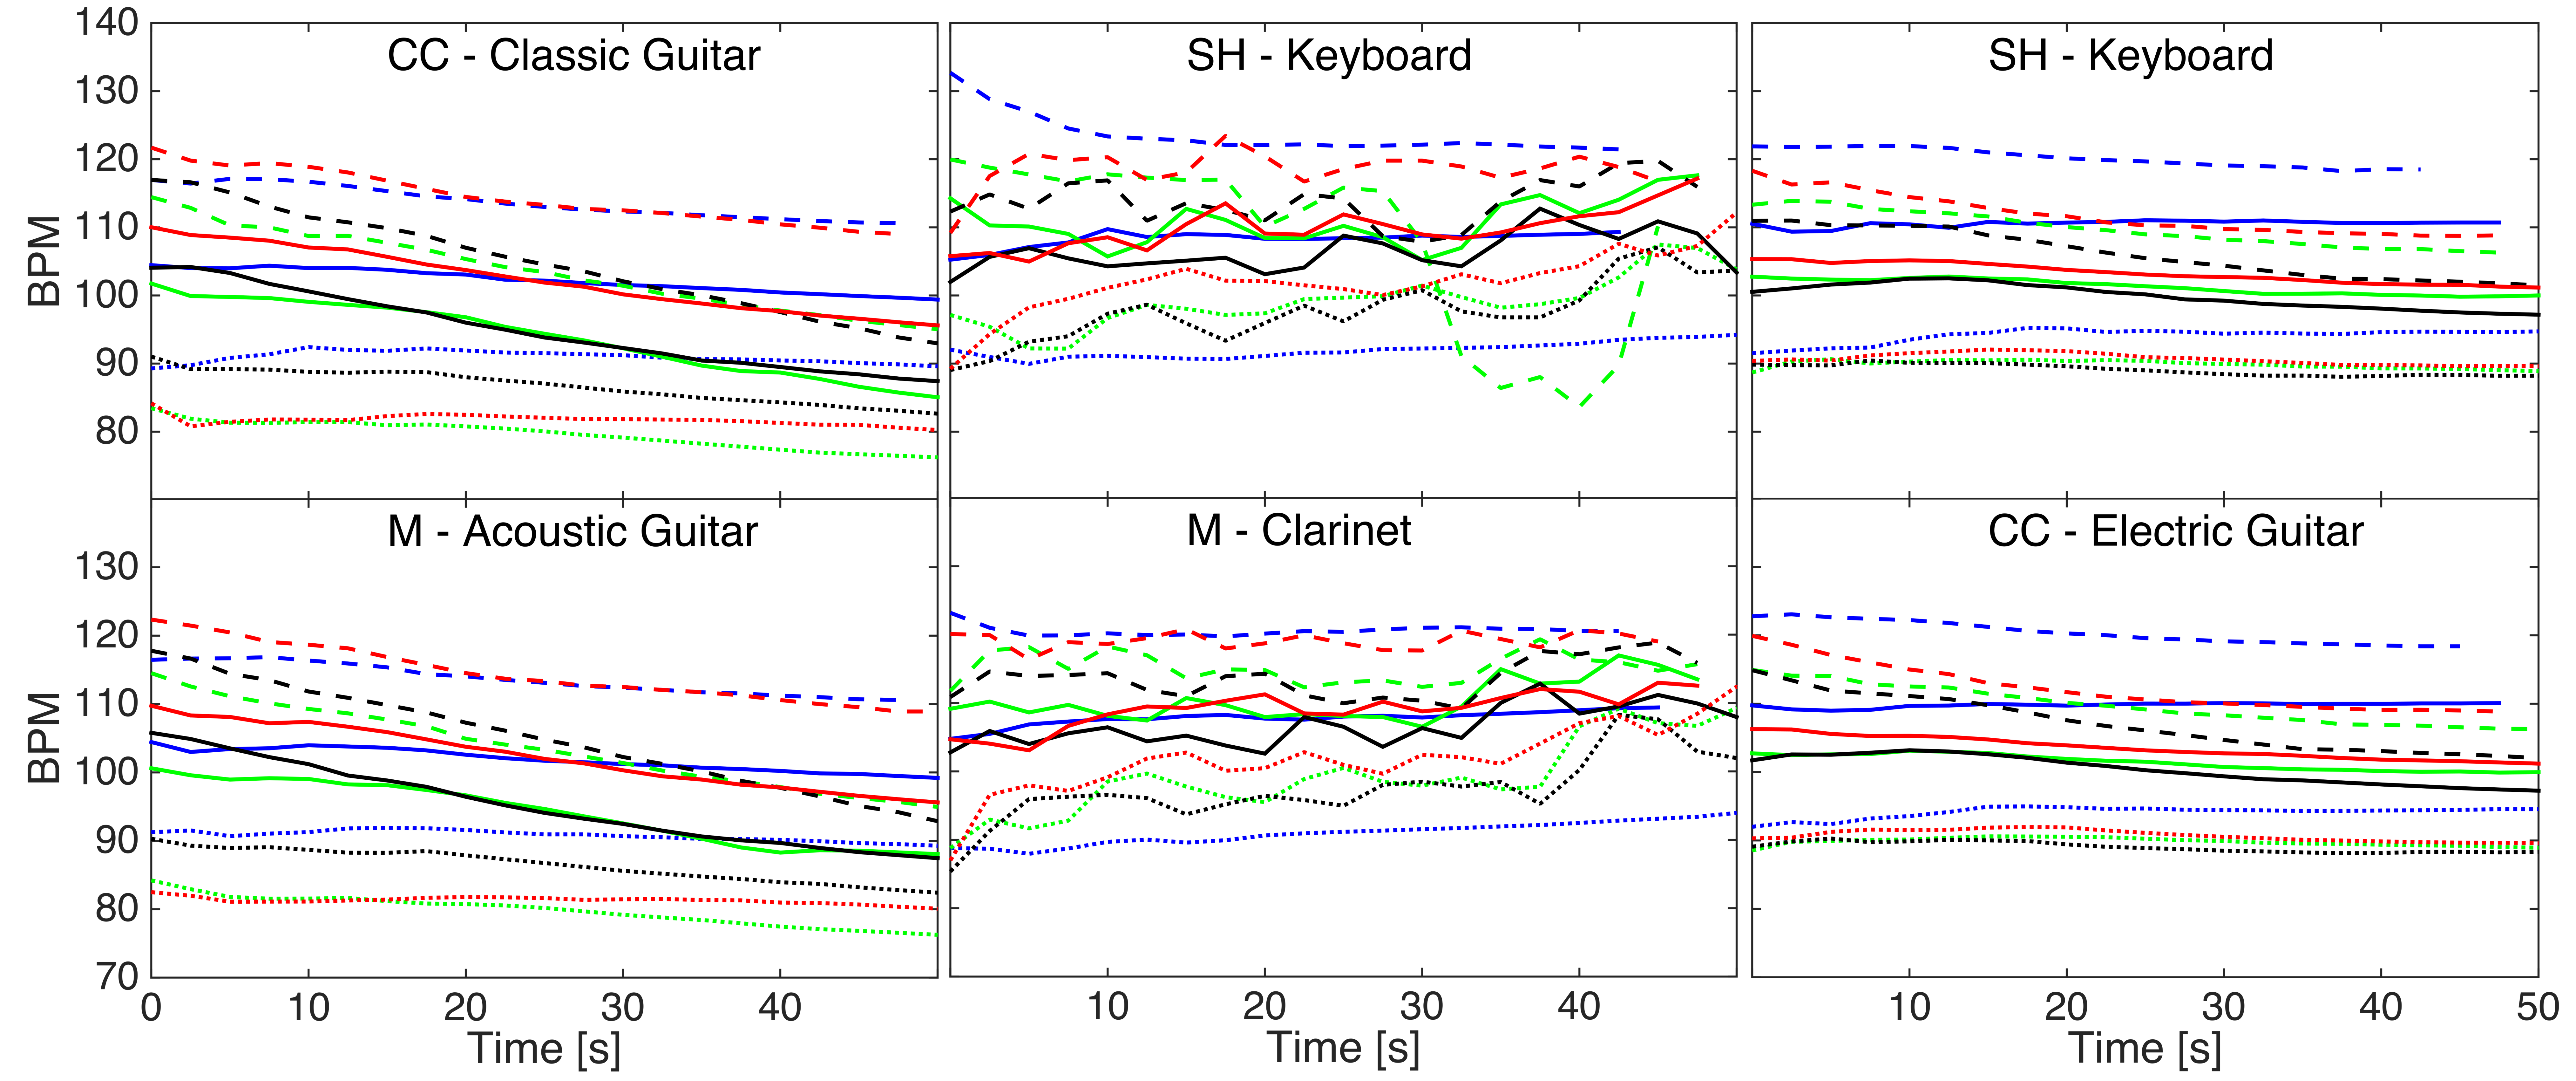
\includegraphics[width=\textwidth]{img/NMP/fig1_wider}\label{fig:NMP:melody}}  
		\hfil
		\subfloat[Combinations for the Drum part with the Chord Comping, the Sustained Harmony and the Melody parts]{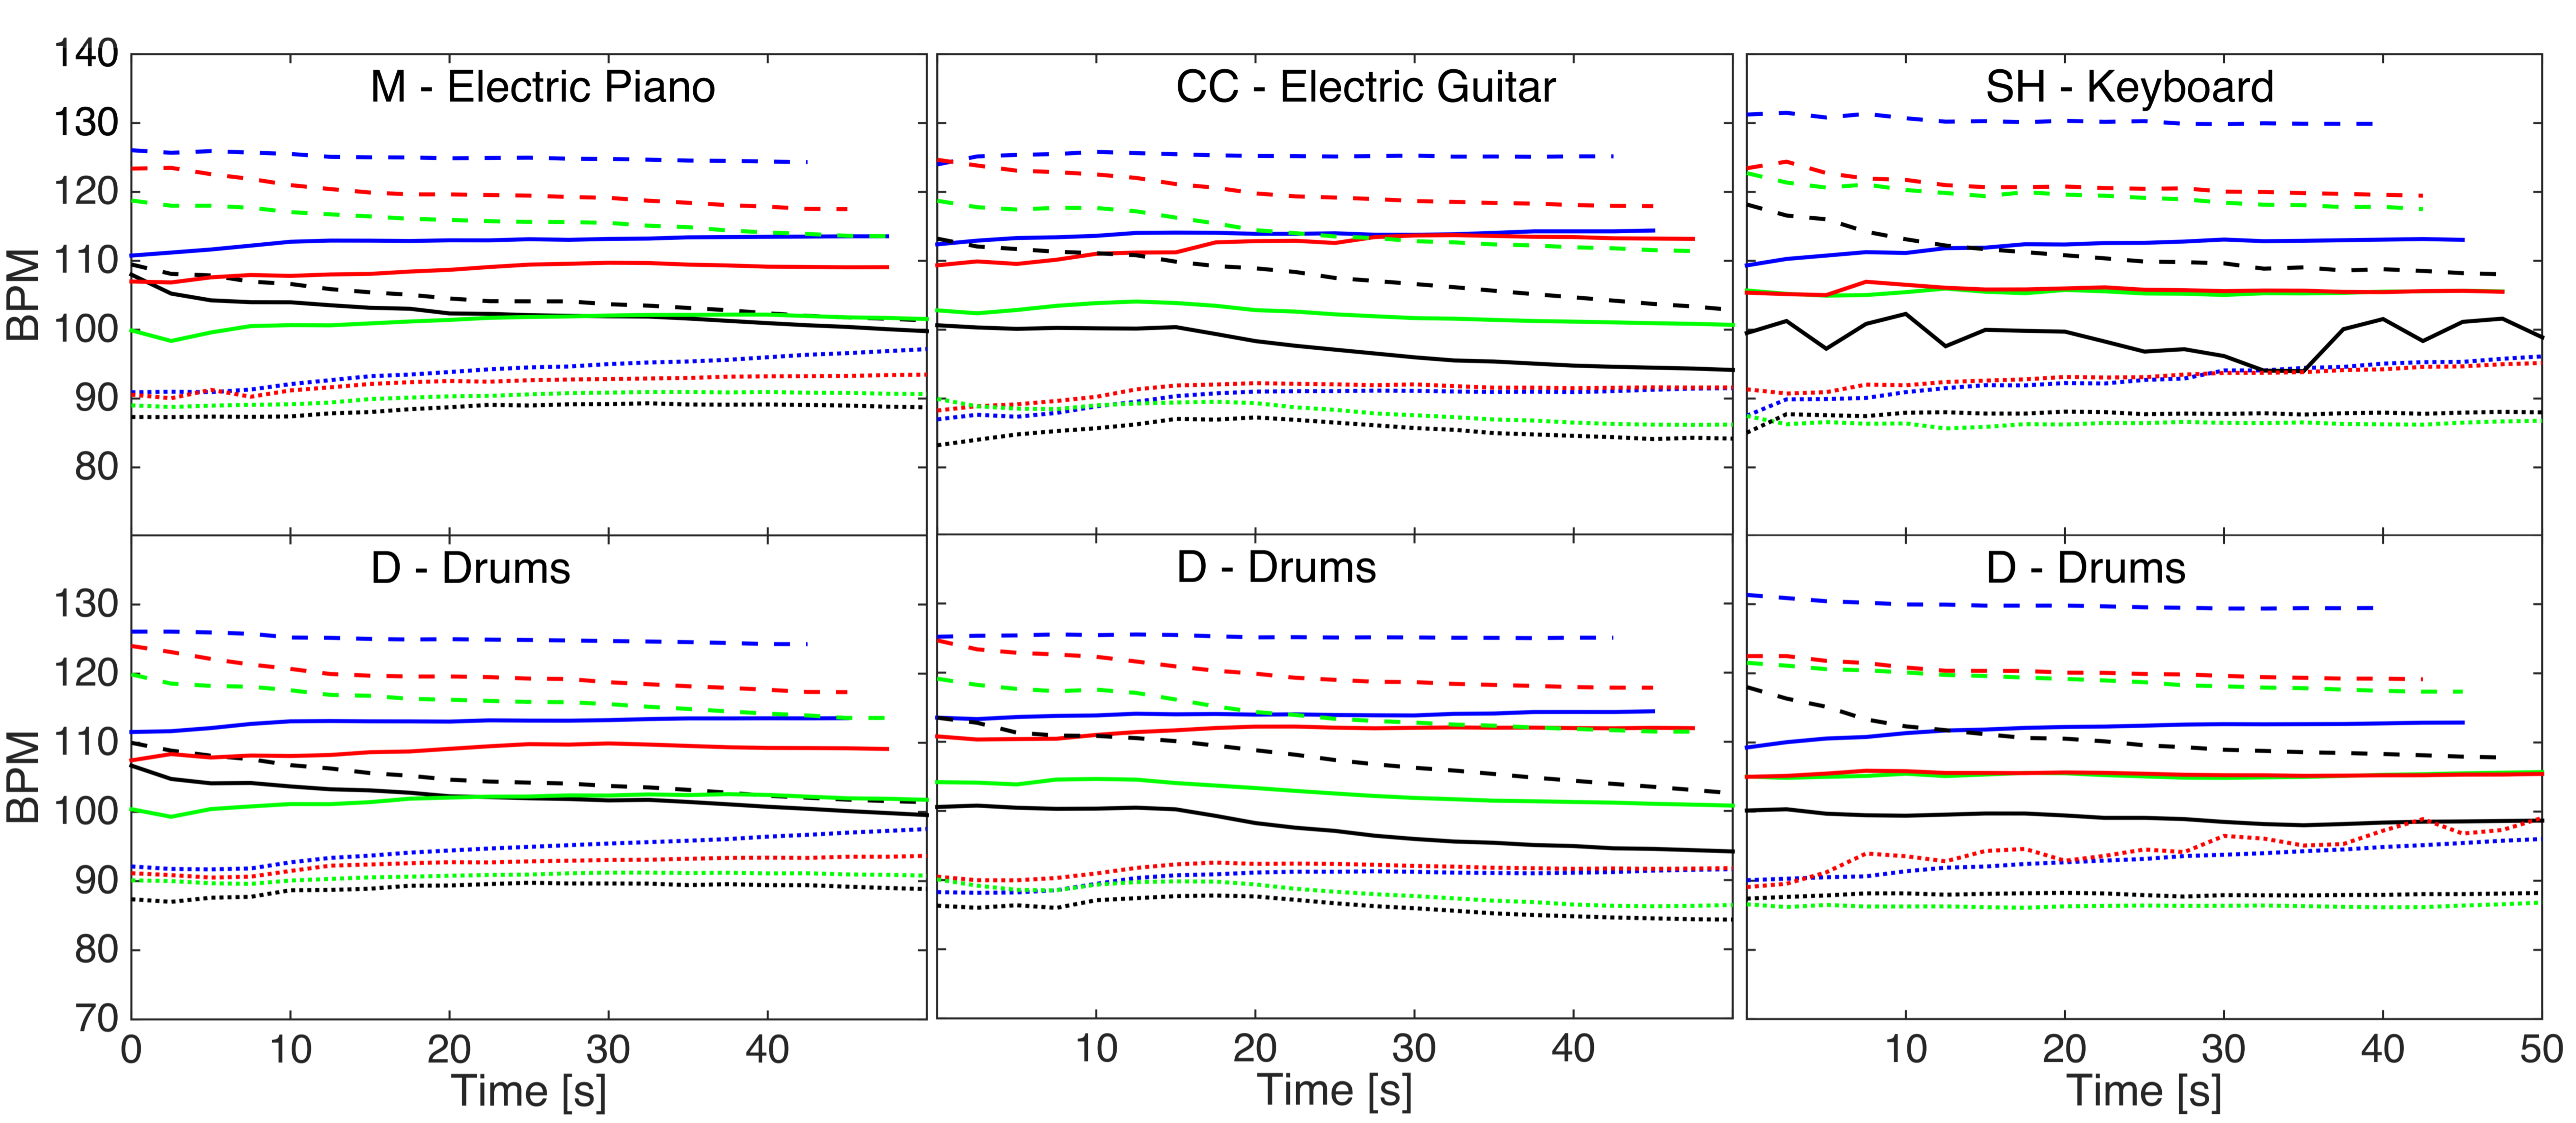
\includegraphics[width=\textwidth]{img/NMP/fig2_wider}\label{fig:NMP:drums}}%\centering
\caption{BPM trend over time when playing \textit{Yellow Submarine}, for different combinations of parts, instruments, end-to-end delays $T_{tot}$ (identified by the color) and reference BPMs $\delta$, identified by the type of line (solid, dashed, dotted). }
\label{fig:NMP:qualTot}
\end{figure}

\begin{figure}[!th]
	\centering
	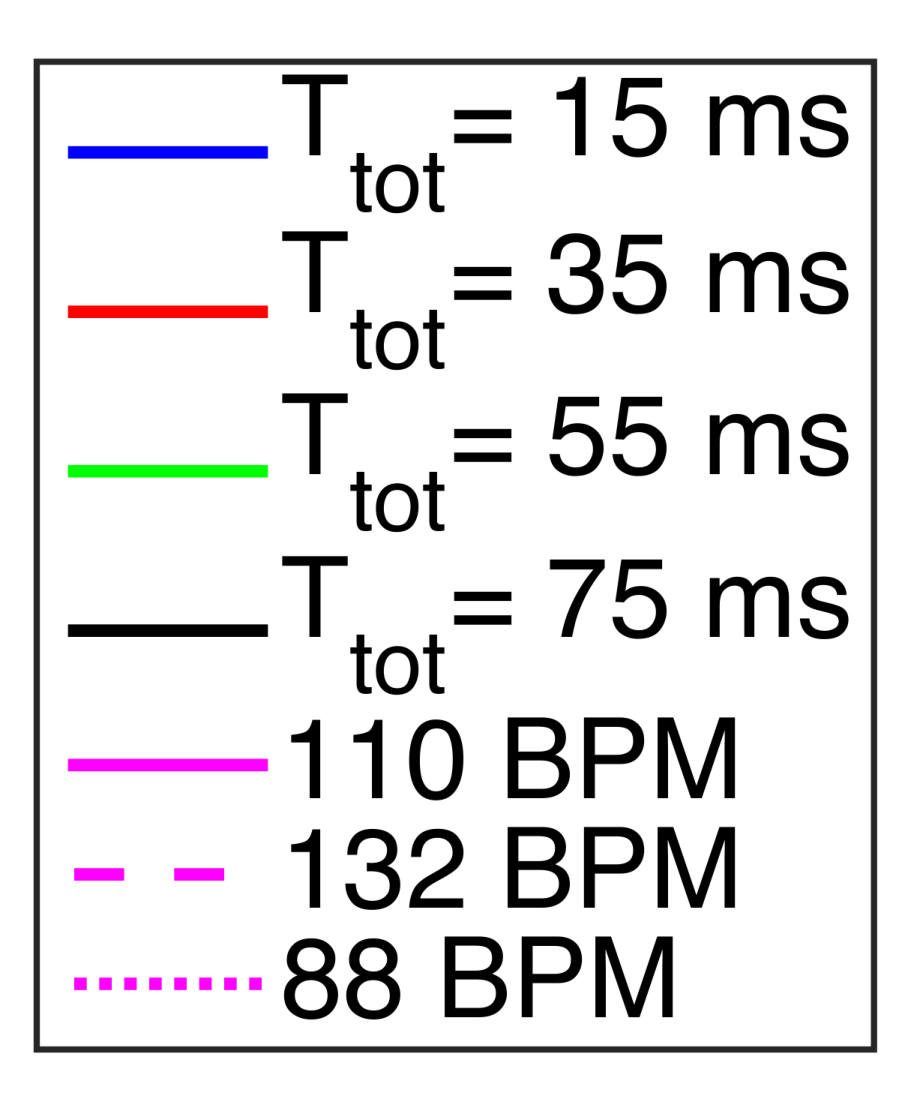
\includegraphics[width=0.2\textwidth]{img/NMP/legend_smaller}
	\caption{Legend for Figures \ref{fig:NMP:melody} and \ref{fig:NMP:drums} }
	\label{fig:NMP:legend} 
\end{figure}


When two homo-rhythmic parts (those that are expected to keep a steady tempo, such as CC and SH) are combined, $b(t_n)$ tends to remain almost constant (see Figure \ref{fig:NMP:melody}, on the right-hand side, where a slight negative slope occurs only at $\delta=132$ BPM).
A similar behavior is observed when M, CC or SH combine with Drums (See Figure \ref{fig:NMP:drums}), despite the fact that the two parts are not always homo-rhythmic. This is due to the fact that drums tend to have a very specific rhythmic ``leading role" in western music, therefore the other musicians generally tend to follow the drummer.

Based on the above results, we conclude that the choice of the combination of instruments and parts has a significant impact on the capability of the musicians to keep a steady tempo. 
In the next Section, we will give a more in-depth analysis of the impact of single rhythmic and timbral features characterizing the specific combination of parts and instruments on the subjective and objective performance quality metrics.

\subsection{Quantitative evaluation}\label{sec:NMP:quantResults}
We now analyze the impact of different end-to-end delays $T_{tot}$ on the subjective quality metric $D_{perc}$ and on the BPM slope $\kappa$, for various values of the rhythmic and timbral features described in Section \ref{sec:NMP:domain}. The interaction quality rating $Q_{perc}$ resulted to be strongly correlated to $D_{perc}$, therefore for the sake of brevity we do not report such results.


%\subsubsection{Dependency of Quality Metrics on Rhythmic Features}
\begin{figure}[!tb]
\begin{flushright}
  \subfloat[Subjective Perception of Delay $D_{perc}$]{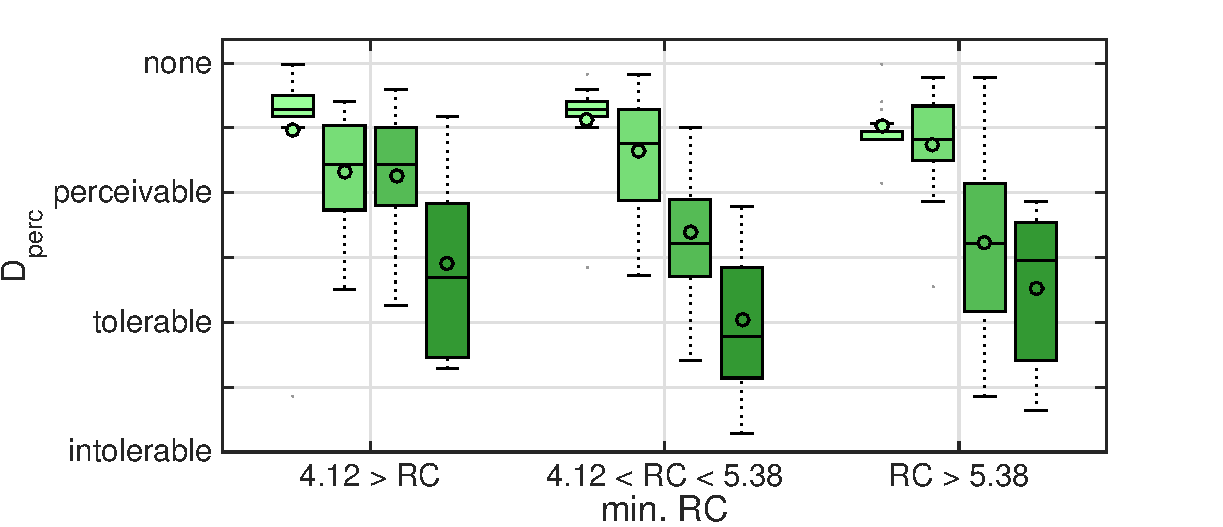
\includegraphics[width=.77\textwidth]{img/NMP/minRC_PD}\label{fig:NMP:minRC_SubjPerc}}  \hfil
  \subfloat[Average BPM Linear Slope $\kappa$]{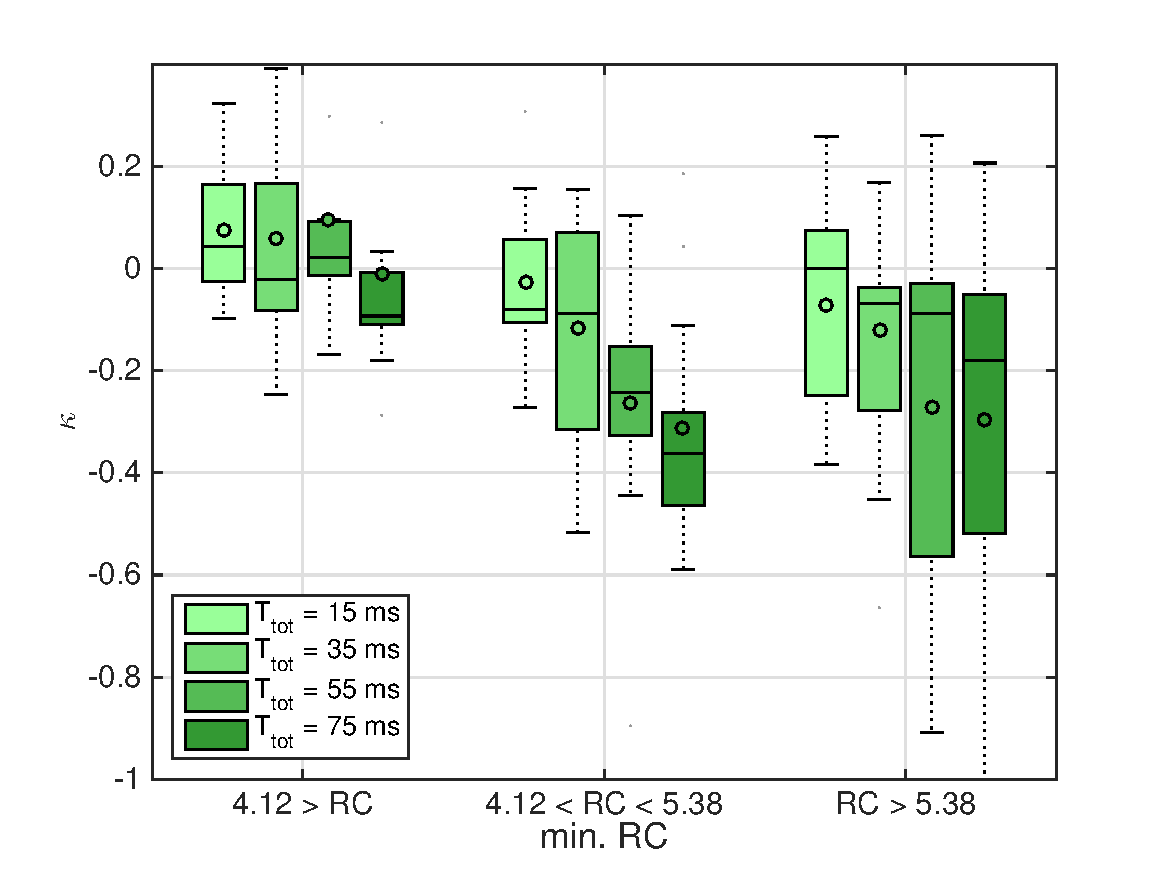
\includegraphics[width=.72\textwidth]{img/NMP/minRC_BPM}\label{fig:NMP:minRC_LinSlope}}        
\end{flushright}
\caption{Dependence of $\kappa$ and $D_{perc}$ on the minimum Rhythmic Complexity $RC$ for different values of $T_{tot}$.}
\label{fig:NMP:minRC}
\end{figure}


 

For every recording, we consider the maximum and minimum values of each feature among the two parts and instruments played by the musicians. For example, in test session 2 (see Table \ref{tab:NMP:sessions}) when performing \textit{Bolero}, the minimum Event Density ($ED$) is 2.01 ($ED$ of the D part) and the maximum $ED$ is 2.14 ($ED$ of the M part). Conversely, the minimum Rhythmic Complexity ($RC$) is 5.53 (on the M part) and the maximum $RC$ is 6.03 (on the D part).

\begin{figure}[!tb]
\begin{flushright}
  \subfloat[Subjective Perception of Delay $D_{perc}$]{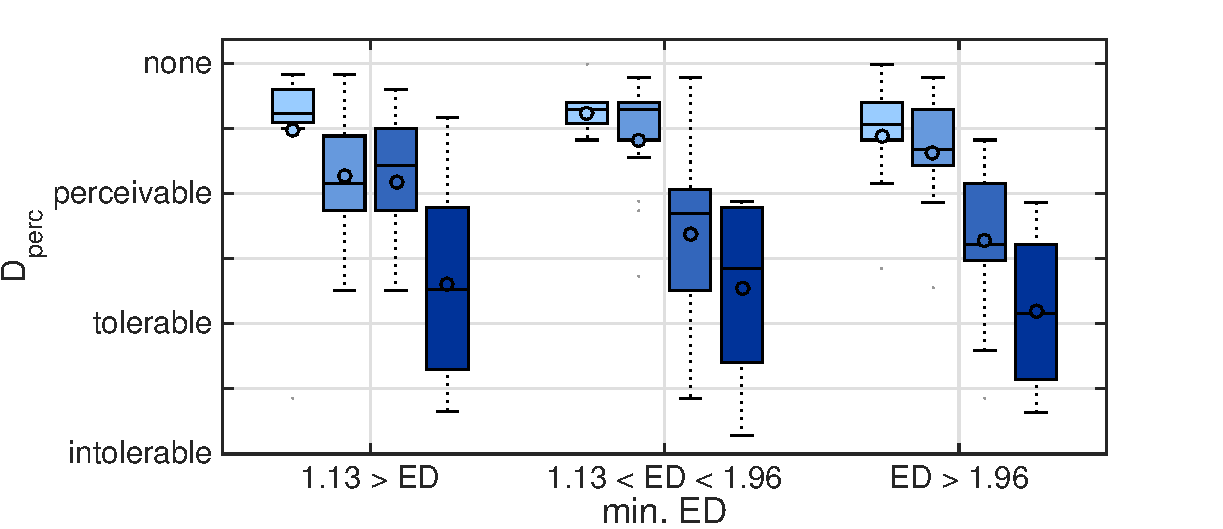
\includegraphics[width=.77\textwidth]{img/NMP/minED_PD}\label{fig:NMP:minED_SubjPerc}}  \hfil
  \subfloat[Average BPM Linear Slope $\kappa$]{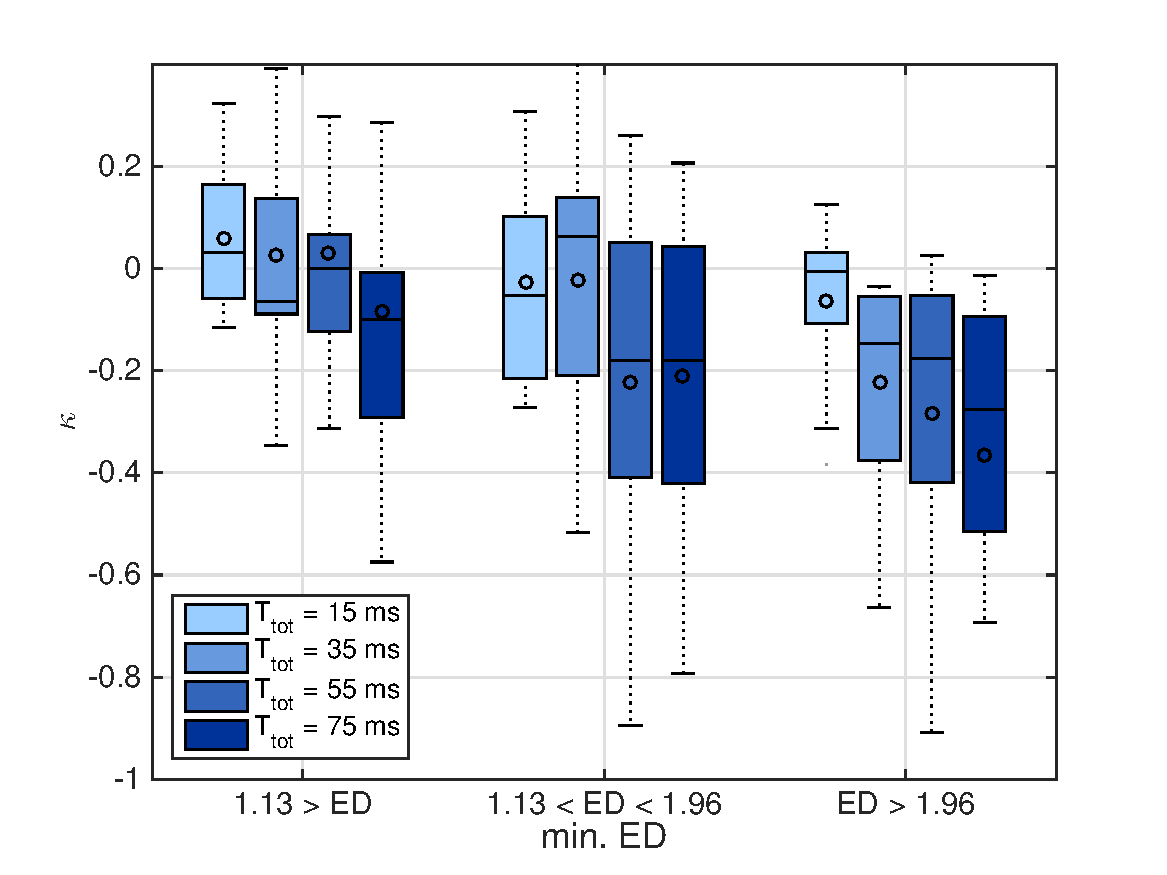
\includegraphics[width=.72\textwidth]{img/NMP/minED_BPM}\label{fig:NMP:minED_LinSlope}}        
\end{flushright}
\caption{Dependence of $\kappa$ and $D_{perc}$ on the minimum Event Density $ED$ for different values of $T_{tot}$}
\label{fig:NMP:minED}
\end{figure}

Figure \ref{fig:NMP:minRC_SubjPerc} reports the subjective delay perception $D_{perc}$ attributed by the pairs of testers to their performances, for different values of $T_{tot}$, as a function of the minimum $RC$ between the two parts. For the sake of clarity, only four values of $T_{tot}$ are reported, where $T_{tot}=T_{proc}=15$ ms is considered as benchmark. 

\begin{figure}[!tb]
\begin{flushright}
  \subfloat[Subjective Perception of Delay $D_{perc}$]{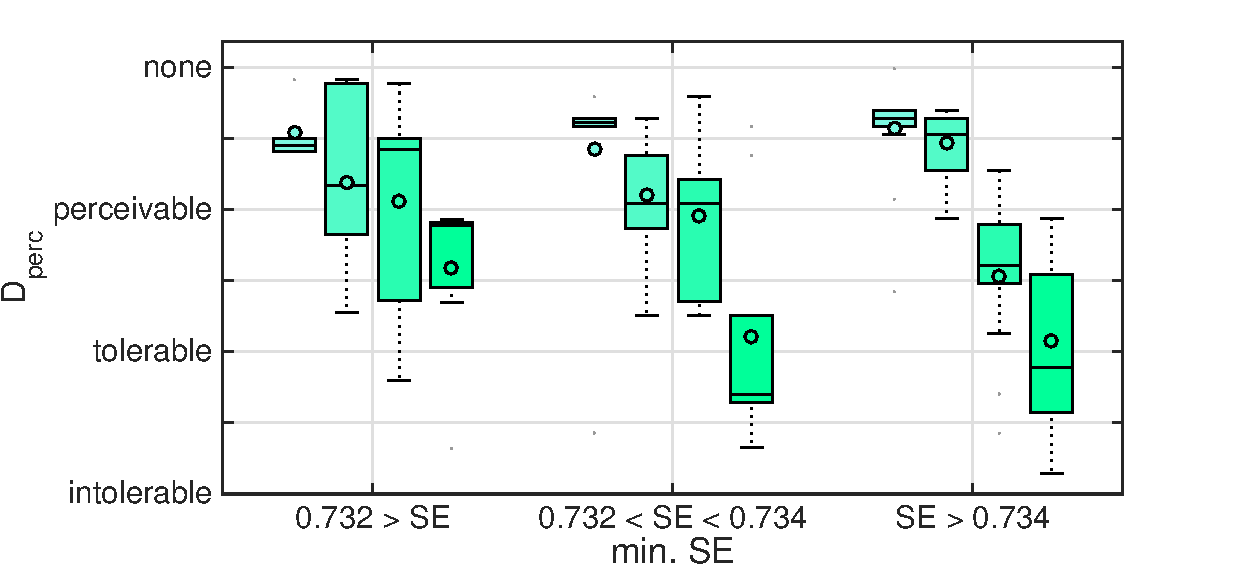
\includegraphics[width=.77\textwidth]{img/NMP/minSE_PD}\label{fig:NMP:minSE_SubjPerc}}  \hfil
  \subfloat[Average BPM Linear Slope $\kappa$]{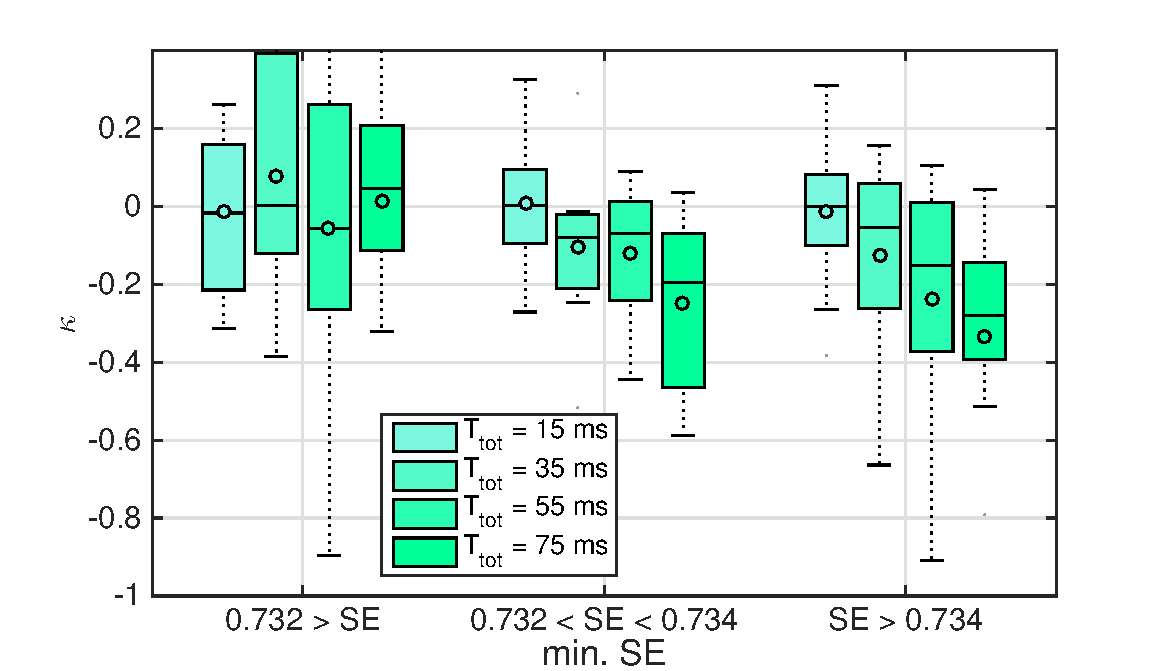
\includegraphics[width=.72\textwidth]{img/NMP/minSE_BPM}\label{fig:NMP:minSE_LinSlope}}        
\end{flushright}
\caption{Dependence of $\kappa$ and $D_{perc}$ on the minimum Spectral Entropy $SE$ for different values of $T_{tot}$}
\label{fig:NMP:minSE}
\end{figure}


Results show that, for a given value of minimum $RC$, the average $D_{perc}$ decreases when $T_{tot}$ increases. Moreover, for a given $T_{tot}$, increasing $RC$ also has a negative impact on the average quality rating. However, the reduction of $D_{perc}$ is more enhanced for large values of $T_{tot}$. 
%Similar results are obtained when considering the subjective delay perception $D_{perc}$, averaged over the pair of performers (see Figure \ref{}).

\begin{figure}[!tb]
\begin{flushright}
  \subfloat[Subjective Perception of Delay $D_{perc}$]{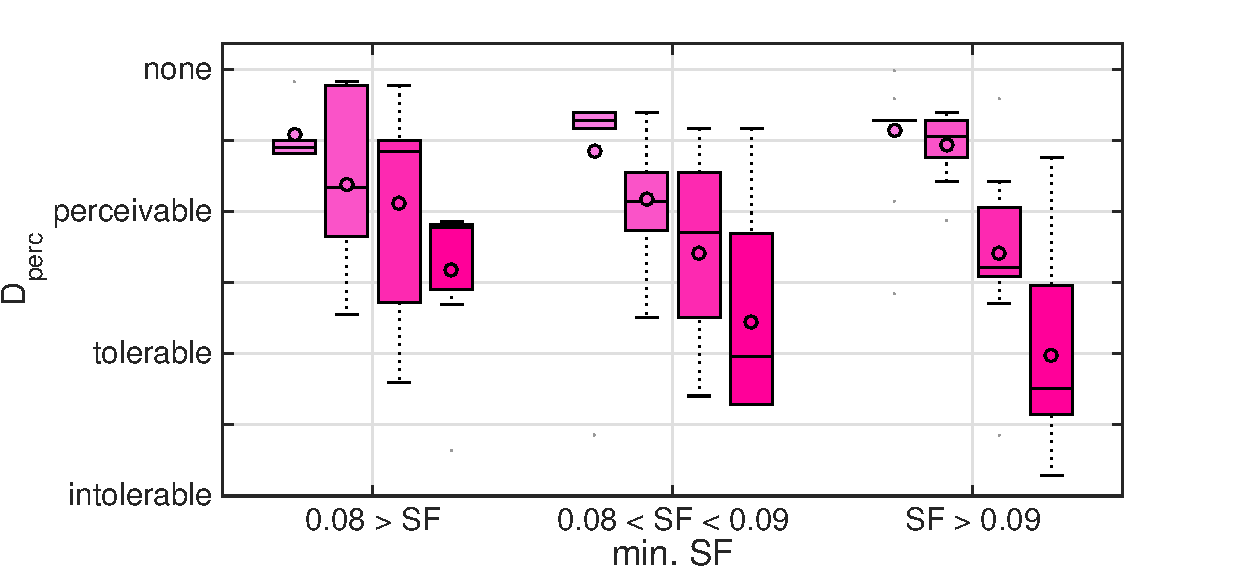
\includegraphics[width=.77\textwidth]{img/NMP/minSF_PD}\label{fig:NMP:minSF_SubjPerc}}  \hfil
  \subfloat[Average BPM Linear Slope $\kappa$]{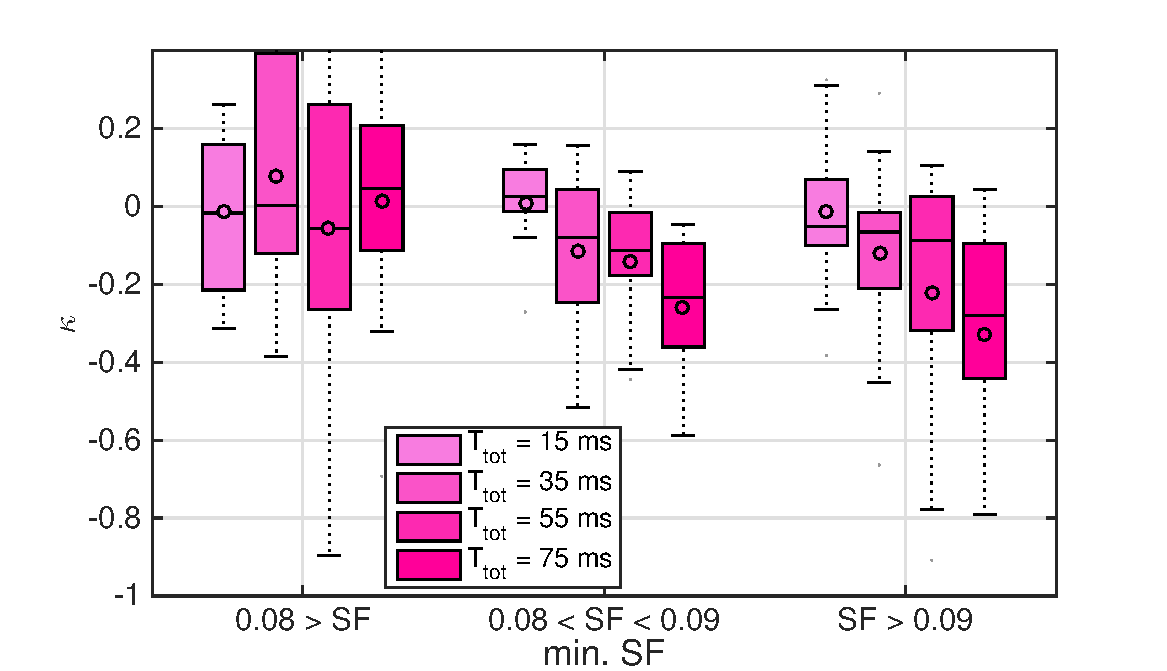
\includegraphics[width=.72\textwidth]{img/NMP/minSF_BPM}\label{fig:NMP:minSF_LinSlope}}        
\end{flushright}
\caption{Dependence of $\kappa$ and $D_{perc}$ on the minimum Spectral Flatness $SF$ for different values of $T_{tot}$}
\label{fig:NMP:minSF}
\end{figure}

We now analyze how the average BPM linear slope $\kappa$ is affected by the minimum rhythmic complexity $RC$. For large values of $RC$ (see Figure \ref{fig:NMP:minRC_LinSlope}), we found slightly negative values of $\kappa$ (which denote a tendency to slow down) even in the benchmark scenario. As expected, the need of synchronism increases when musicians are playing more complex parts and the lack of typical synchronization cues, such as eye-contact, affects the performance even in absence of network delay. However, negative slopes tend to become much steeper for large values of $T_{tot}$, which suggests that the tolerance to the delay decreases for more complex musical pieces.

\begin{figure}[!tb]
\begin{flushright}
  \subfloat[Subjective Perception of Delay $D_{perc}$]{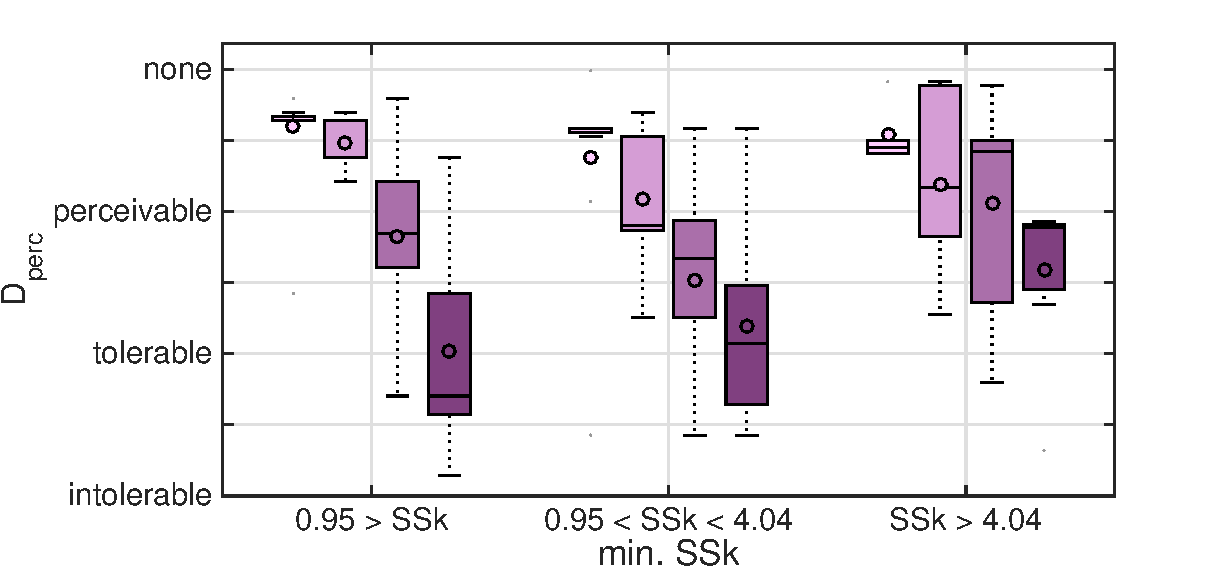
\includegraphics[width=.77\textwidth]{img/NMP/minSSk_PD}\label{fig:NMP:minSSk_SubjPerc}}  \hfil
  \subfloat[Average BPM Linear Slope $\kappa$]{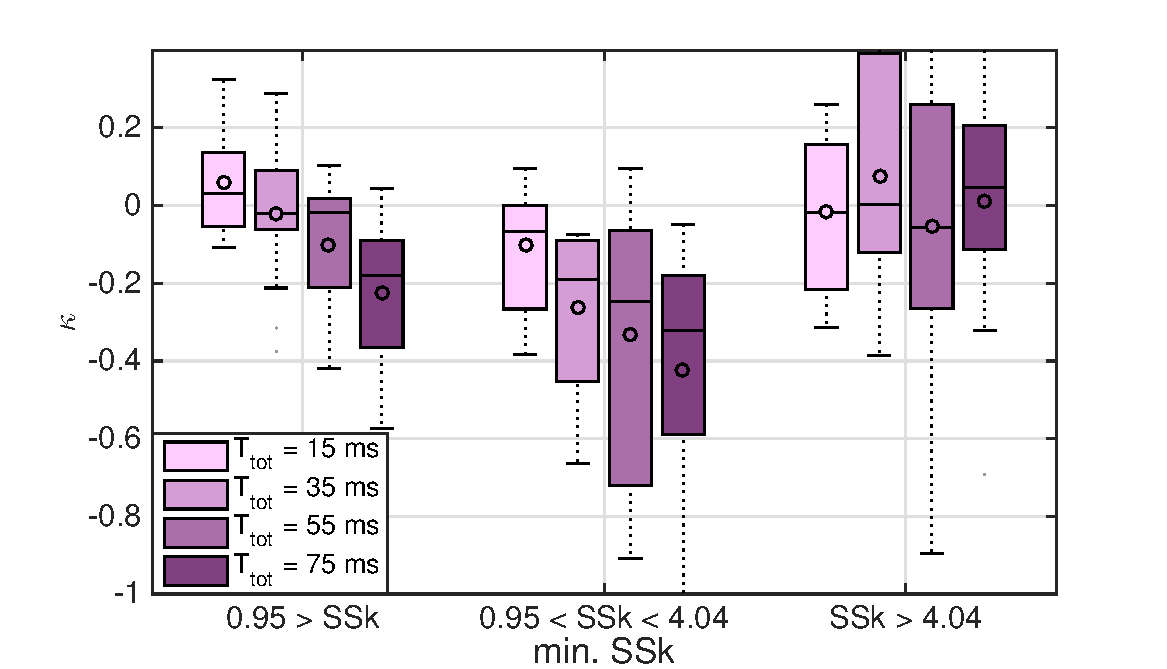
\includegraphics[width=.72\textwidth]{img/NMP/minSSk_BPM}\label{fig:NMP:minSSk_LinSlope}}        
\end{flushright}
\caption{Dependence of $\kappa$ and $D_{perc}$ on the minimum Spectral Skewness $SSk$ for different values of $T_{tot}$}
\label{fig:NMP:minSSk}
\end{figure}

Similar conclusions can be drawn on the dependence of the perceived delay $D_{perc}$ and the objective metrics $\kappa$ on the minimum $ED$, as depicted in Figure \ref{fig:NMP:minED}, due to the non-negligible correlation that exists between $RC$ and $ED$. 
These conclusions remain substantially unvaried if, instead of considering the minimum values of $RC$ and $ED$, we consider the maxima.
%\subsubsection{Dependency of Quality Metrics on Timbral Features}

\begin{figure}[!tb]
\begin{flushright}
  \subfloat[Subjective Perception of Delay $D_{perc}$]{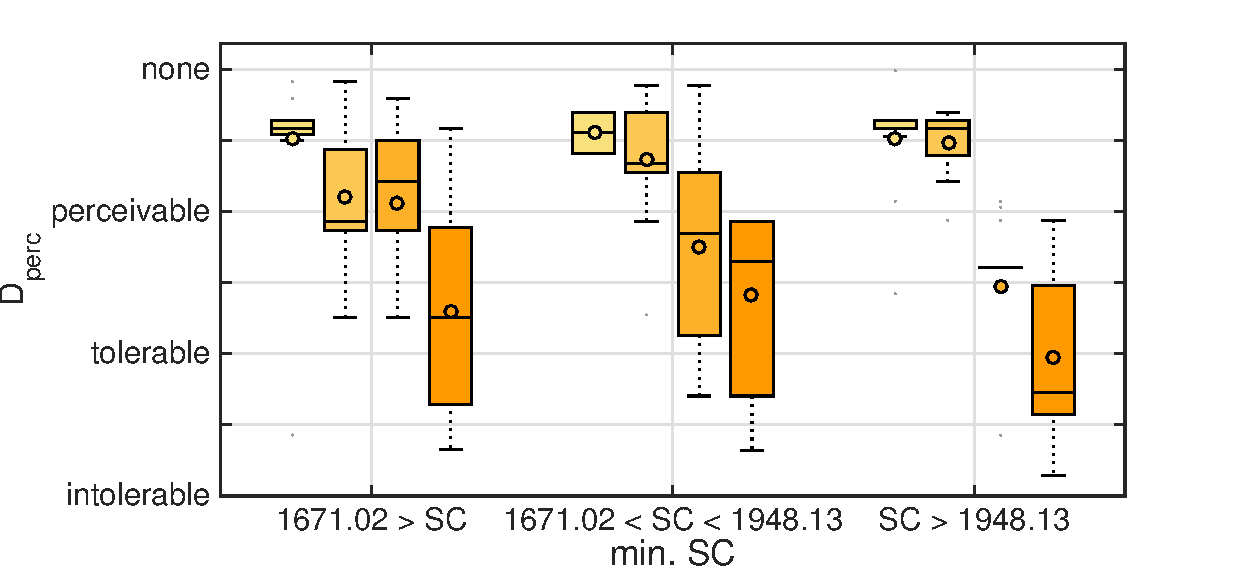
\includegraphics[width=.77\textwidth]{img/NMP/minSC_PD}\label{fig:NMP:minSC_SubjPerc}}  \hfil
  \subfloat[Average BPM Linear Slope $\kappa$]{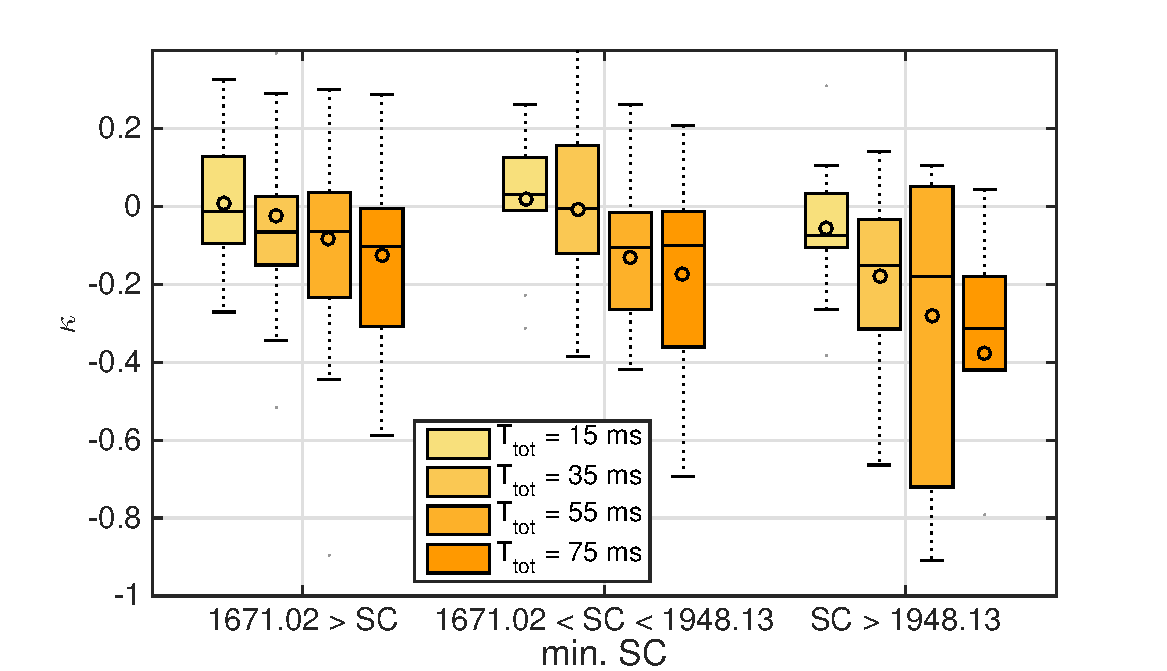
\includegraphics[width=.72\textwidth]{img/NMP/minSC_BPM}\label{fig:NMP:minSC_LinSlope}}        
\end{flushright}
\caption{Dependence of $\kappa$ and $D_{perc}$ on the minimum Spectral Centroid $SC$ for different values of $T_{tot}$.}
\label{fig:NMP:minSC}
\end{figure}


With respect to the timbral features, we observe that the noisiness of the instrument, which is captured by Spectral Entropy, Flatness and Spread, negatively affects the perceived delay $D_{perc}$. For example, in Figures \ref{fig:NMP:minSE} and \ref{fig:NMP:minSF} we show $D_{perc}$ and $\kappa$ are affected by Spectral Entropy ($SE$) and Spectral Flatness ($SF$). We consider the minimum Entropy and minimum Flatness between the two involved instruments. Focusing on the objective metric $\kappa$ (see Figures \ref{fig:NMP:minSE_LinSlope} and \ref{fig:NMP:minSF_LinSlope}), we notice that as the $SE$ and the $SF$ increase, the tempo  slowdown becomes more accentuated. This impact is negligible for low network delays, but it grows significantly for fairly large values of $T_{tot}$. Similar considerations are valid for $D_{perc}$, as reported in Figure \ref{fig:NMP:minSE_SubjPerc}. Analogous findings also apply to the dependency of the quality metrics on the Spectral Spread and here not reported for the sake of brevity.  

Conversely, when considering the impact of Spectral Skewness ($SSk$) and Spectral Kurtosis ($SK$) on the performance metrics, we notice that, for a given delay $T_{tot}$, a change in their values does not lead to a change in the quality to perceivably worsen (see Figure \ref{fig:NMP:minSSk}, results on $SK$ not reported for conciseness). 

Finally, when looking at the influence of the Spectral Centroid $SC$ (i.e., of sound brightness) on the subjective quality metrics, results reported in Figure \ref{fig:NMP:minSC_SubjPerc} show that the perceptual metric $D_{perc}$ does not exhibit significant fluctuations due to a varying $SC$. However, for large values of $SC$, a slight tendency to decelerate emerges in Figure \ref{fig:NMP:minSC_LinSlope}, which shows the impact of $SC$ on the objective quality metric $\kappa$.

It is also worth remembering that $D_{perc}$ is not necessarily an objective indicator of quality degradation of the performance, but only on the musicians' subjective perception of the end-to-end delay. For example, two musicians might keep a steady tempo ($\kappa=0$) even if they perceive a high and intolerable network delay. However, from results reported in Figures \ref{fig:NMP:minRC_SubjPerc}, \ref{fig:NMP:minED_SubjPerc}, \ref{fig:NMP:minSE_SubjPerc}, \ref{fig:NMP:minSF_SubjPerc}, \ref{fig:NMP:minSSk_SubjPerc}, \ref{fig:NMP:minSC_SubjPerc}, we can assume that such perception is strongly affected by the timbral and rhythmic characteristics of the combination of instruments and parts. For example, in Figure \ref{fig:NMP:minSSk_SubjPerc}, the perceived network delay $D_{perc}$ is higher for $SSk>4.04$ and $T_{tot}=75 ms$ than the value we would have with the same delay in the case of lower Skewness. This leads us to think that the musicians' capability of estimating the network delay is biased by the perceived interaction quality of the performance. 
This means that large network delays (i.e., $T_{tot}\geq 75ms$) do not prevent networked musical interaction, but they limit the selection of the instrument/part combinations. Thus, the resulting experience can be satisfactory if the performer is willing to trade flexibility and perceived interaction quality with the convenience of playing over the network.

\subsection{Final considerations for the Networked Music Performance}\label{sec:NMP:conclusions}
In this Section, we have discussed the ability of LLFs and MLFs representing and analyzing the music signals in the context of Networked Music Performance.
%the effectiveness of LLFs and MLFs for the formalization of the signal domain, i..e, their ability of representing and analyzing the music signals. In order to develop a better understanding of the (low-level) semantics that is carried by these features, we conducted a research activity in the context of Networked Music Performance.
This particular activity has proven that the understanding of the hand-crafted features is crucial to address the problems that regard the signal domain.  We have in fact performed an extensive evaluation of the quality of NMPs as a function of numerous parameters, some concerning telecommunication network delays and conditions, others involving rhythmic and timbral descriptors of the musical instruments involved. The analysis also considers the influence of the role of the instrument on such quality metrics.

We have found that the possibility of enjoying an interactive networked musical performance is not only a function of the total network delay, but it also depends on the role and the timbral characteristics of the involved musical instruments, as well as the rhythmic complexity of the performance. When playing more rhythmically complex pieces, musicians exhibit a more pronounced tendency to decelerate for higher network latencies. Nonetheless, the rhythmical complexity does not significantly worsen their perception of the delay and of the interaction quality.
Among the timbral features, instruments with a higher Spectral Entropy and Spectral Flatness (such as guitars and drums) lead to larger tempo slowdown in case of higher network delays. In addition, they also amplify the negative impact of network delay on the perceived delay and interaction quality.

With these results in mind, we are able to estimate the network constraints for a NMP given the combination of parts and instruments that are performing remotely.

%
%The NMP is a promising application to allow musicians to jam and compose songs from different physical location through the network. The network connections introduce a delay that musicians must take into account. While several network architectures can be proposed in order to reduce such delay, it is important to understand which factors affect the musicians' tolerance to it and which conditions make it easy for musicians to remotely perform.
%In order to conduct this analysis, we implemented a testbed for psycho-acoustic tests, which emulates the behavior of a real telecommunication network in terms of variable transmission delay and jitter. %, and we quantitatively evaluated the impact of the various performance parameters on the trend of the tempo that the musicians were able to keep during the performance, as well as on the perceived quality of the musical interaction.
%We model the analysis of factors that affect NMP as a linking function between the low-level and mid-level interpretation of the signal domain and the semantics expressed by the perceived and objective quality of the performance. The former allows us to objectively analyze the role of rhythmic complexity in the parts, as well as the timbral properties of the instruments that are played. The latter provides both a subjective and an objective evaluation of the performance. We use a manual analysis of the correlation between the two domains to understand which factors of the music performance are involved.




\section{Learned Features}\label{sec:LLFs:learned}
The hand-crafted and model-based features have been widely used in the MIR literature to extract a representation of the signal domain by employing signal processing techniques, psychoacoustic and musicological models. The use of such features requires to know in advance which characteristics are involved from the musical content and which features are able to extract such characteristics, which is not always feasible. In such situations, a typical approach is to extract all the possible features and evaluate their correlations with the desired output. However, it is possible that the features cannot extract the characteristics that matter for the specific issue and, therefore, it is necessary to identify a method to automatically extract a salient representation of the signal domain. In order to do so, we might want to mimic the human ability of organizing and elaborating the information from music.

% ----- The goal of Deep Learning -----
Recent neurological studies have shown that the human brain describes concepts (information) in hierarchical fashion \cite{Serre2007}. Indeed, the brain seems to process information through multiple stages of transformation and representation, providing multiple levels of abstraction \cite{Haykin1998}. The process is inducted by the physiological deep architecture of the mammal brain, where each level corresponds to a different area of cortex \cite{Serre2007}. As an example, in a simplistic form, while listening to a piano playing a melody, our brain first collects acoustic stimuli like frequency spectra and energy distributions. These pieces of information are then combined to build more complex concepts like the sequence of notes and the piano timbre. Notes, at the same time, are used to infer the concept of melody.

For this reason, the decomposition of decisional problems into sub-problems associated with different levels of abstraction results to be very effective \cite{Humphrey2013}. The analysis of the signal domain shall mimic this ability, but the extraction of hand-crafted features does not exploit enough depth \cite{Bengio2009}. This is why deep learning has been receiving great attention in the last few years.

Deep learning techniques attempt to emulate the human brain representation of information by providing several layers of analysis \cite{Bengio2009}. This is typically done by using a multi-layer structure such as neural networks. The input of the network represents the data under analysis (the spectrum of an audio frame in our case), and the output of each layer is a representation of the input (the \textit{learned} features in our case) obtained through processing (characteristic of the deep learning network). The more the layers, the \textit{deeper} the network and the higher the reached level of abstraction.


\begin{figure}[t]
\captionsetup[subfigure]{justification=centering}
	\centering
%      \subfloat[Input]{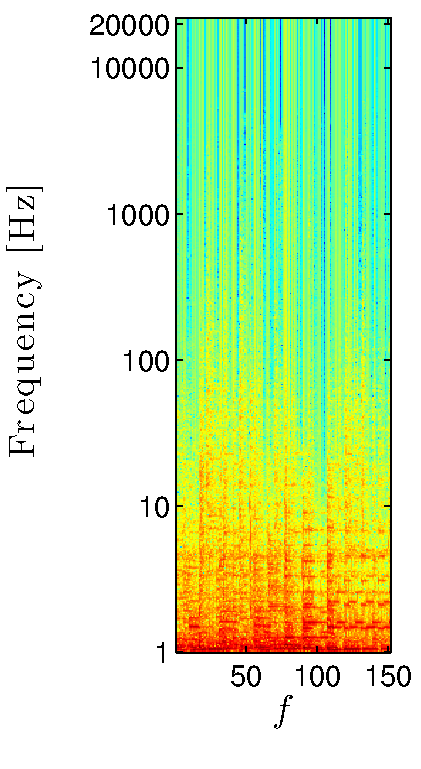
\includegraphics[width=.45\textwidth]{img/Bootleg/original_input}\label{fig:LLFs:input}} \hfil
      \subfloat[Original spectrogram]{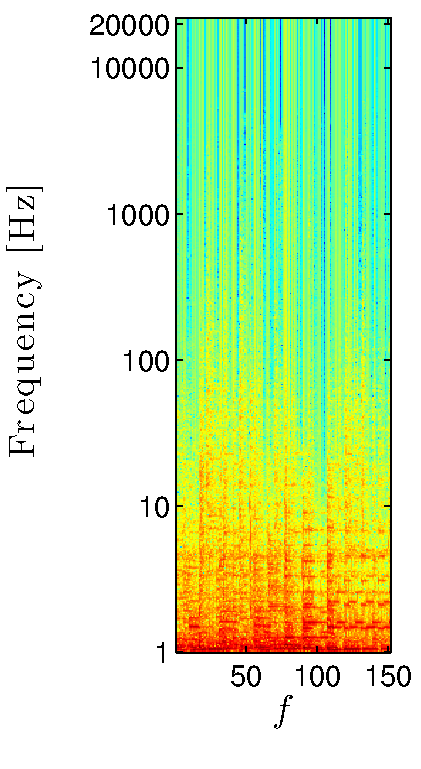
\includegraphics[trim=0cm 0cm 0cm 0cm,clip=true,totalheight=0.65\columnwidth]{img/Bootleg/original_input}\label{fig:LLFs:input}} \hfil
      \subfloat[Spectrogram reconstructed from the first layer]{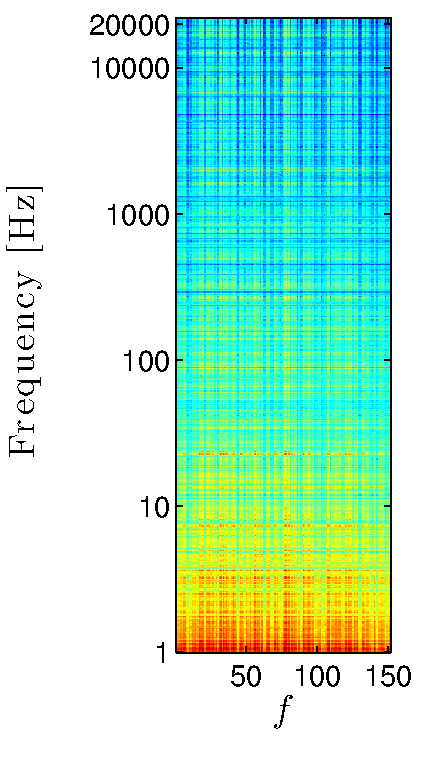
\includegraphics[trim=2.9cm 0cm 0cm 0cm,clip=true,totalheight=0.65\columnwidth]{img/Bootleg/first_layer}\label{fig:LLFs:first}}
      \subfloat[Spectrogram reconstructed from the second layer]{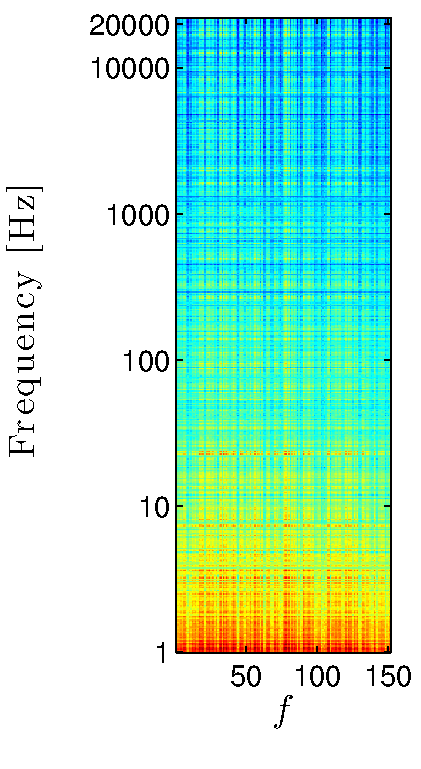
\includegraphics[trim=2.9cm 0cm 0cm 0cm,clip=true,totalheight=0.65\columnwidth]{img/Bootleg/second_layer}\label{fig:LLFs:second}}
      \subfloat[Spectrogram reconstructed from the third layer]{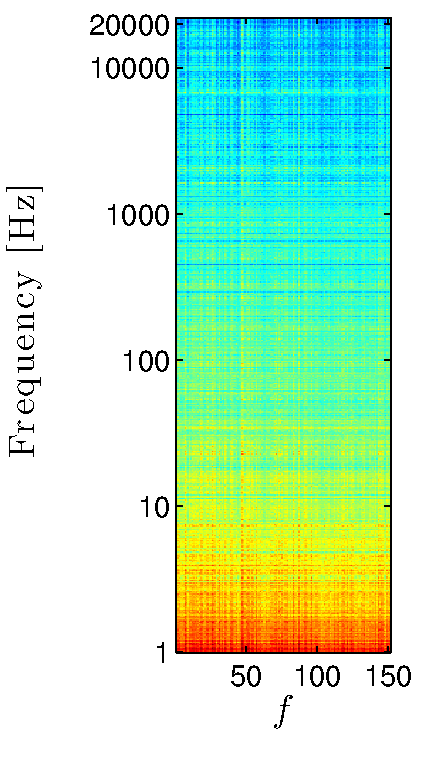
\includegraphics[trim=2.9cm 0cm 0cm 0cm,clip=true,totalheight=0.65\columnwidth]{img/Bootleg/third_layer}\label{fig:LLFs:third}}            
      \caption{A song spectrogram reconstructed from different layers of a deep learning network}
      \label{fig:LLFs:features}          
\end{figure}


Unlike hand-crafted features, features learned using deep learning methods are not easily interpretable since there is not a clear mapping with specific acoustic cues. To show the input characteristics captured by the learned features, it is possible to invert the process and reconstruct the input starting from the features. As an example, Figure \ref{fig:LLFs:features} shows a song spectrogram, and its reconstructed versions starting from learned features at different abstraction layers. We notice that, at each layer, only characteristic frequencies of the spectrum are preserved, whereas less informative bands tend to be discarded. It is also possible to further process the reconstructed spectrograms and to obtain a reconstructed waveform. In \cite{choi2015auralisation}, the authors perform an \textit{auralization} of single neurons in order to empirically infer which properties the neurons captured. Some examples of interpretation include onset detector, kick drum detector and bass note selector. 

Deep learning techniques perform non-linear transformations to input data in order to learn and extract salient information. Such techniques do not need to know in advance the target application of the extracted features, and therefore they extract a generic representation of the distribution of the input domain. For this reason, such techniques are named \textit{unsupervised} deep learning techniques, and the extracted features are referred to as \textit{unsupervised learned features}. Nevertheless, deep learning network can be also \textit{fine-tuned} in order to learn a target-oriented representation, i.e., a representation that is more useful for a given task.
 
%In particular, unsupervised deep learning techniques are able to learn and extract salient information from unlabeled data, i.e., from generic data of which they do not know any prior perform non-linear transformations to input data in order to learn and extract salient information in an unsupervised fashion. This technique is particularly suitable for feature learning process. %Although even a one-layer unsupervised learning algorithm could extract salient features, it has a limited capacity of abstraction. For this reason, a multi-layer approach can be used. Each layer is fed using the output of the lower-layer and each layer is designed to give a more abstract representation of the previous layer activations. In this way, higher-level abstractions that characterize the input could emerge.


\begin{figure}[tbp]
	\centering
	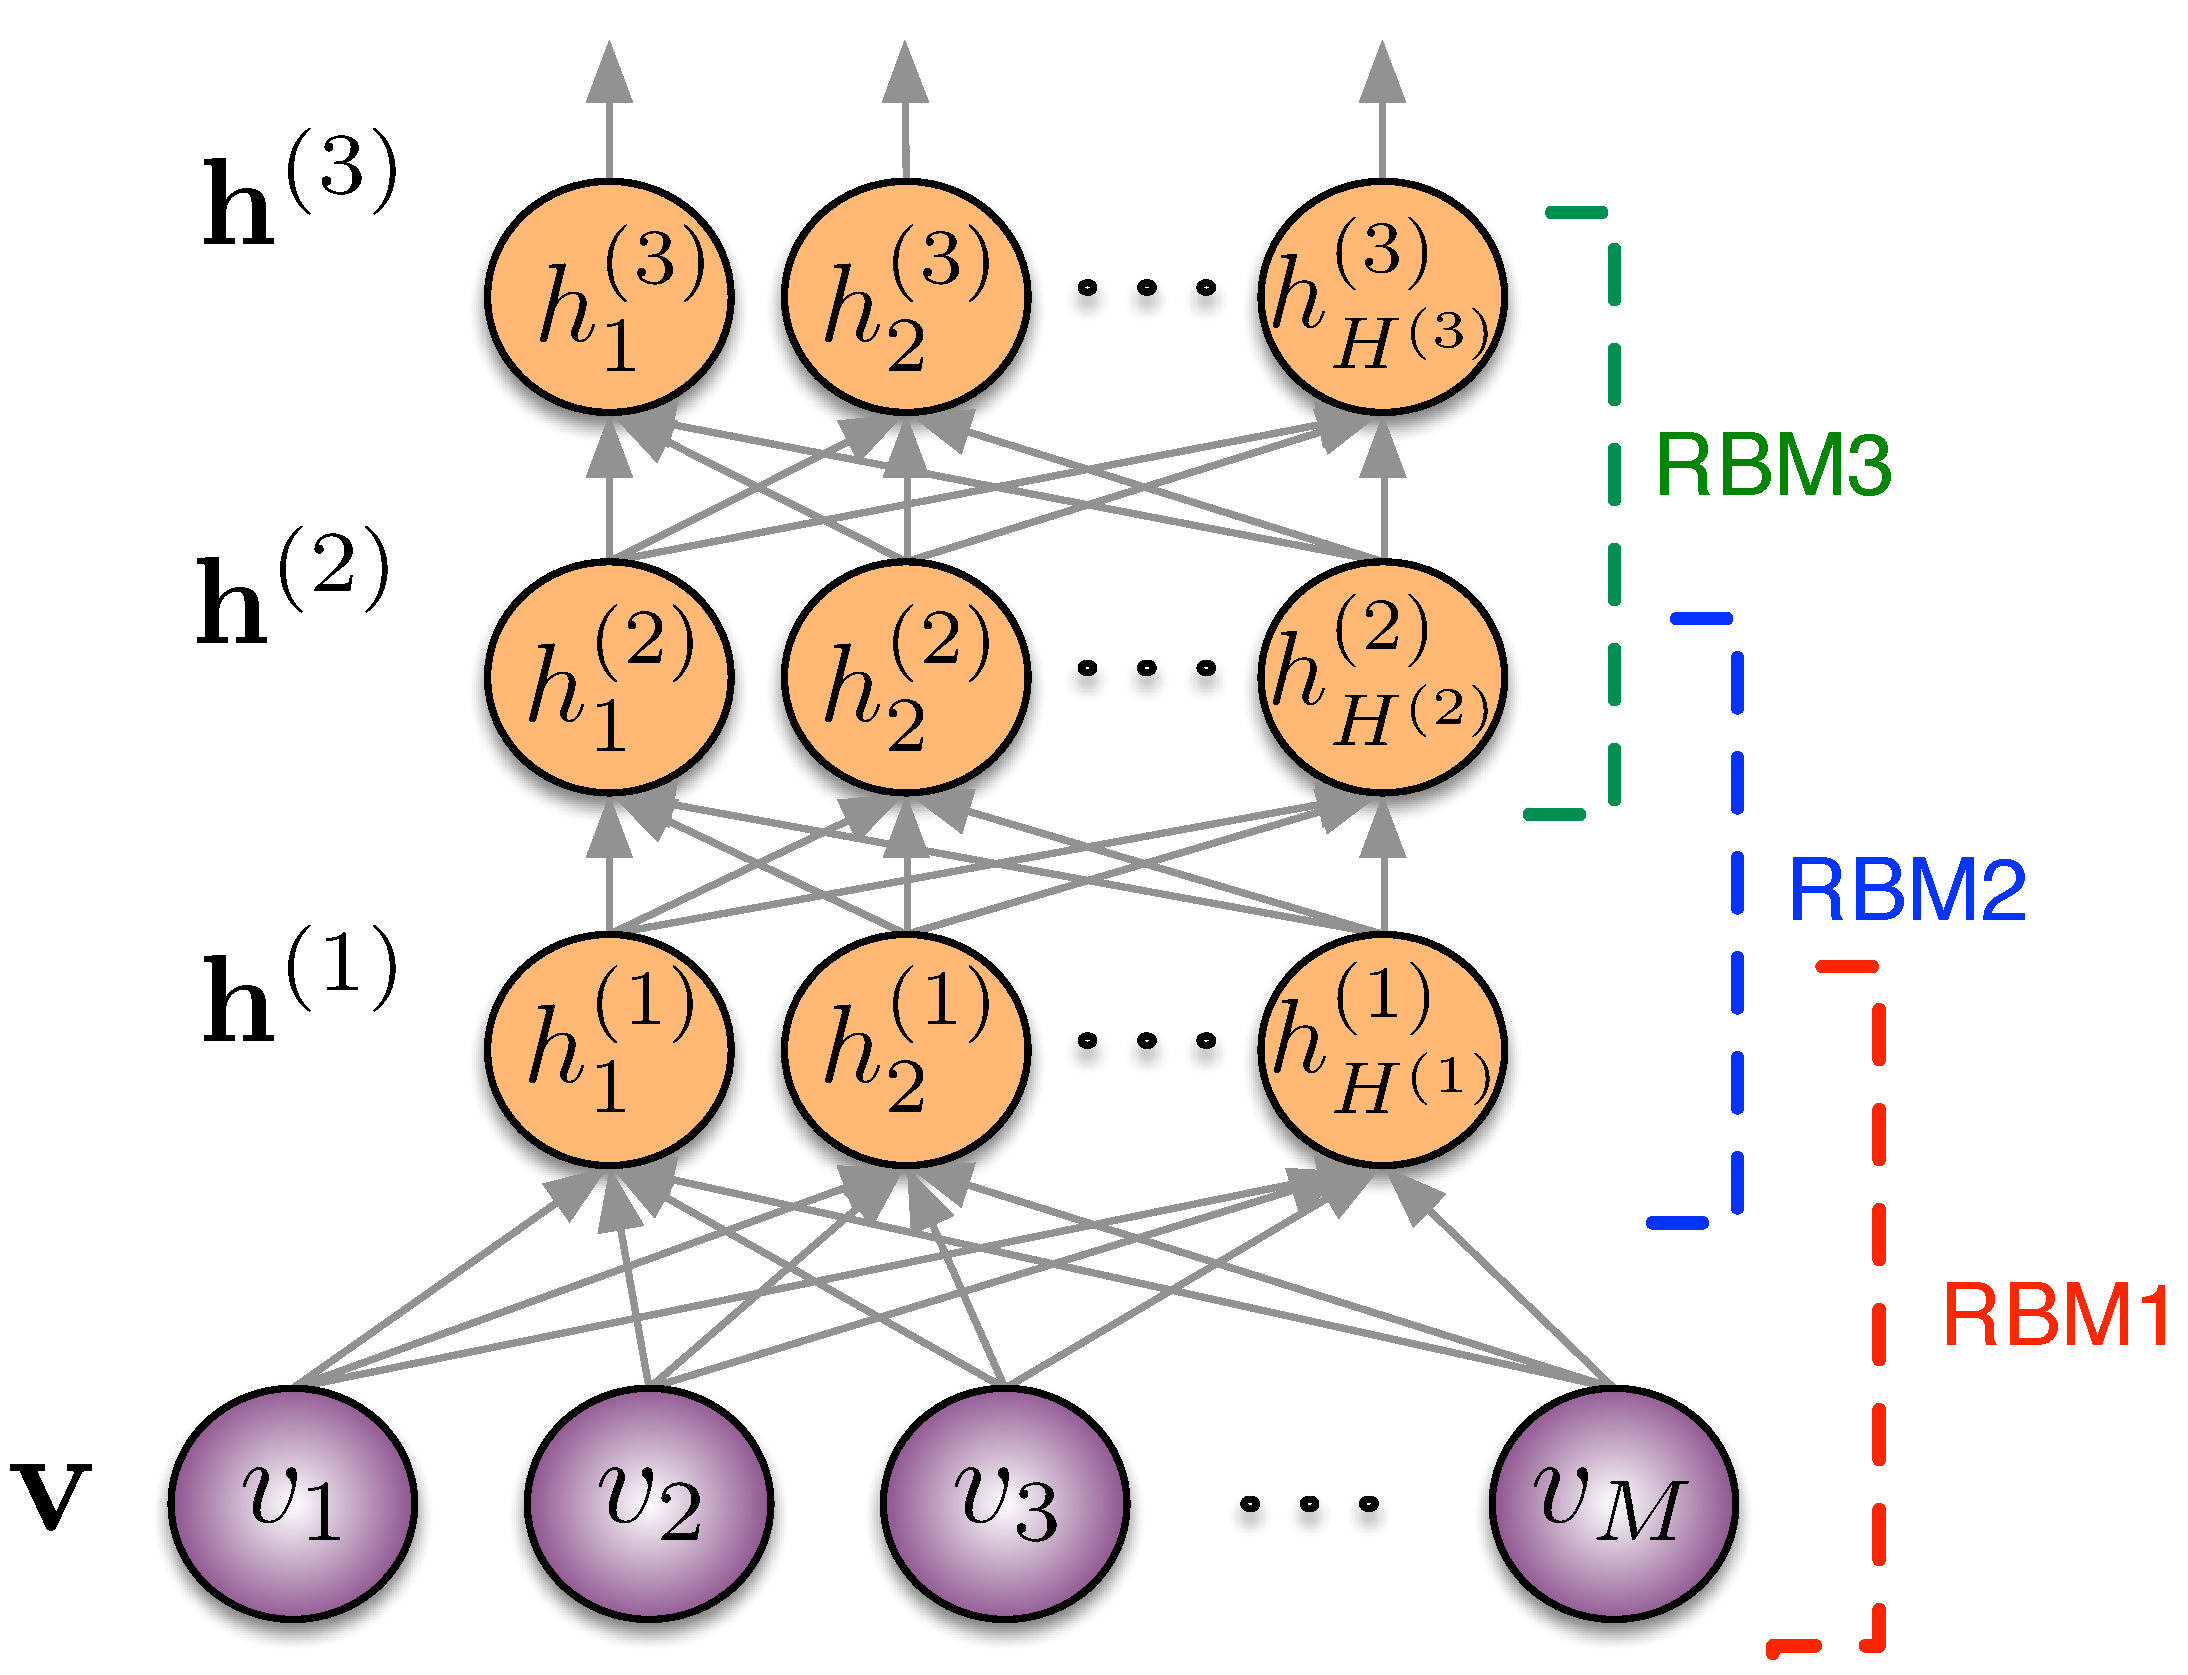
\includegraphics[width=.6\textwidth]{img/MSA/deep.pdf}
	\caption{General representation of a DBN}
	\label{fig:LLFs:DBN}
\end{figure} 


In our work we focus on a deep architecture named \textit{Deep Belief Network} (DBN), which is a multilayer neural network composed of simpler neural networks named \textit{Restricted Boltzmann Machines} (RBMs).
An RBM is a two-layer neural network that models the probability distribution of an input variable. The first layer represents the input, whose distribution is encoded by means of the second layer, which is referred to as \textit{hidden layer} \cite{Bengio2009}. The hidden layer is therefore used as a representation of the input layer.
In a DBN, a first RBM models the input distribution by means of the first hidden layer, while the second RBM models the distribution of the first hidden layer into a second hidden layer, and so on through the depth of the DBN \cite{Hinton2006}, as shown in Figure \ref{fig:LLFs:DBN} for a 3-layer DBN. Following Figure \ref{fig:LLFs:DBN}, the lowest level of the DBN, i.e., the one which learns the representation directly from the input ($\mathbf{h}^{(1)}$), is likely to learn features rather related to the signal domain, while the highest level combines the information of the lower levels of information and is able to extract more abstract information.

DBNs have been effectively employed for several tasks, such as musical genre recognition \cite{Hamel2010}, music emotion recognition \cite{Schmidt2011}, and other audio classification problems \cite{Humphrey2013}. In Chapters \ref{Chap:MSA}, \ref{Chap:Bootleg}, \ref{Chap:Violin} we present a set of application scenarios where we use the DBN architecture to automatically extract a feature representation of the signal domain with an unsupervised approach, while in Section \ref{sec:app:learned} we provide a technical overview of the RBM and DBN neural networks.

In the latest years, several other deep architectures have been proposed and tested for the representation of the signal domain. While we do not employ these architectures in our work, it is worth provide a brief overview of their use in the MIR literature.

The autoencoders, or autoassociators \cite{Bengio2009}, are a class of neural networks that use a hidden layer to learn a representation of a visible layer such that the visible layer itself can be reconstructed from the hidden layer. The hidden units are computed as a non-linear transformation of a linear combination of the input units, which can be the sigmoid function or other non-linear functions. A popular non-linear transformation is the Rectified Linear Unit (ReLU) that is defined as $f(x)=\text{max}(0,x)$, which has the advantage of being piecewise linear, hence easily tractable for the computation of the gradient \cite{Zeiler2013}. Before training an autoencoder, some noise can be added to the input, in order to avoid overfitting issues and enforce the training of the network (\textit{denoising autoencoders} \cite{vincent2008extracting}). By stacking several layers of autoencoders together, with an approach similar of the DBNs, we obtain a deep learning architecture named \textit{stacked autoencoders}. Denoising stacked autoencoders have been employed in Music Information Retrieval by \cite{maillet2009steerable} to extract a music representation for the automatic generation of playlists.

DBNs and stacked autoencoders usually work on a frame-level representation of the audio input, attempting at capturing the salient features. This approach does not take the evolution of the features over time into consideration. Two main deep architectures which include time information in the model are: the Recurrent and the Convolutional Neural Networks.

The Recurrent Neural Networks (RNNs) are able to learn a representation of the input that takes the time dimension into account by keeping memory of the past samples. In order to do so, they take as input both the data of the current frame and some information on the previous ones. More formally, given an instant $t$, which is represented by a time-frame input $x_t$, the network computes the hidden representation of the frame $h_t=f(x_t, h_{t-1})$, where $f$ is the generic function for the generation of the output (usually a non-linear function of a linear combination of the input). The presence of $h_{t-1}$ as input is important because it is itself generated as $f(x_{t-1}, h_{t-2})$, i.e., it encodes information from the previous samples \cite{mesnil2013investigation}. The RNNs are usually learned through a supervised training step to learn a representation oriented for a task. The RNNs have quickly achieved and sometimes outperformed the state-of-the-art performance in several MIR tasks, such as beat tracking \cite{bock2014multi}, music transcription \cite{sigtia2016end} or emotion recognition \cite{Weninger2014}.

The Convolutional Neural Networks (CNN) have been originally designed for image recognition and have been later used in music information \cite{lee2009convolutional}. The basic idea behind CNNs is to use a filter, named \textit{kernel}, which is convolved with the input in different locations, to collect all the outcome of such filtering and use the pooling of the outcomes as the hidden layer representation. The training step concerns the learning of the weights of the kernel, to obtain a translation-invariant hidden layer representation, due to the pooling of the filtering outcomes from different location. As an example, let us suppose that the input is a set of frames from a spectrogram: depending on the direction of the shifting of the kernel, it is possible to make a CNN either time-invariant or frequency-invariant. This addresses, for example, the problem of detecting whether a certain acoustic event occur in a spectrogram: once the kernel is learned, it will allow the CNN to capture the event in whichever moment it occurs. With the same approach, we detect frequency-shifted acoustic events. The CNNs are in fact highly flexible for the audio analysis whenever the invariance to time or frequency shifting is desirable. For this reason, CNNs have been employed for structural analysis \cite{ullrich2014boundary} as well as music classification \cite{dieleman2011audio}, annotation \cite{dieleman2014end} and recommendation \cite{van2013deep}.

Due to the tremendous impact of  deep learning on the state of the art of machine learning, many frameworks have been proposed for the design and implementation of the architectures. In this work, we use the \textit{Theano} Python library \cite{Bergstra2010}, which provides automatic gradient computation by composing and solving a computational graph derived from the architecture. Other frameworks include Caffe \cite{jia2014caffe} and TensorFlow \cite{tensorflow}.

\section{Final considerations}
The formalization of the signal domain involves the physical world of the sound waves, the perceptual world of the listening and the musicological aspects of the content. Each of this world is composed by several hierarchical layers of complexity and abstraction.

In order to extract a generic representation of the audio signal, or its musical content, we can extract LLFs or MLFs respectively. They are reliable descriptors for the signal domain, which have been manually designed by researchers to capture a specific aspect of the signal. In order to extract them, it is necessary to understand which characteristics matter for the addressing of the problem and which features can capture such characteristics. We conducted a research activity in the context of the Networked Music Performance to highlight how a deep understanding of these features can be effectively used to define the signal domain of a real problem and develop novel solutions.

However, sometimes the needed characteristics are not known in advance and the features who are supposed to capture them do not ensure the required precision. We address these issues by using the deep learning techniques to provide a generic representation of the audio signal with several layers of abstraction. Since we can hardly infer an interpretation of the learned features \cite{choi2015auralisation}, the design effort is shifted from features to architectures. Several architectures have been proposed in the literature and others can be created with ad-hoc solutions that take into account the nature of music. Nevertheless, it was proven that deep learning techniques are effective for extracting a feature representation to address problems related to the signal domain. 

\chapter{Designing the linking function}\label{Chap:ML}
As discussed in previous Chapter \ref{Chap:LLFs}, we formalize the signal domain by means of a feature-based representation. The representation based on hand-crafted and model-based features only provides little insight on the semantics of the music, while the representation based on deep learning architecture requires manual inspection in order to assess its semantics \cite{Le2013,choi2015auralisation}. The semantic domain, which we will  better discuss in the next Chapter \ref{Chap:HLFs}, provides a high-level description of music, that is closer to the way people describe and think of music. The relation between the signal domain, related to the lower-level properties of the musical content, and the semantic domain, related to the high-level interpretation of music, is often not clear, due to the well-known semantic gap between low-level and high-level features \cite{Celma2006}. In this Section, we discuss several techniques that have been employed in the literature to bridge the gap in the Music Information Retrieval research field. 

The design of the linking function involves different techniques, depending on the complexity of the addressed problem and on the available knowledge on the relation between the domains for the specific problem. For some cases, when it is possible to make some assumption on the relation between the two domains, rule-based techniques can be designed and employed. More often, however, the problem that is addressed involves the understanding of the human music's perception, whose modeling is extremely complex and still under investigation. For the latter cases, we take advantage of machine learning techniques to design and train the models for linking function. 

In the following, we provide an overview of the theoretical background and the state of the art of some techniques used in the literature to model the linking function. In Section \ref{sec:ML:data} we first present some basic tools to pre-process the representation of the signal or the semantic domain to help de-noising the data, to improve the effectiveness of the linking function. In Section \ref{sec:ML:kernels} we describe a set of kernel expansion techniques that we used in our work to expand the data and explore possibly underlying patterns within it. In Section \ref{sec:ML:rule-based} we present a set of tools to design rule-based techniques. We focus on the techniques that have been used in the literature to automatically extract the musical structure of songs, since this is a common problem in Music Information Retrieval. Finally, in Section \ref{sec:ML:models} we present a number of machine learning techniques that have been proposed to automatically learn a model for the linking function.

%The design of automatic music mediators can be modeled as a function that links the representation of the signal domain (Chapter ) to the formalization of the semantic codomain (Chapter \ref{Chap:HLFs}). Therefore, the properties of the linking function strongly depend on the two domains. The novel mediator can also be seen as a pipeline that connects the the signal domain to the linking function, and the linking function to the the semantic codomain. From this perspective, the source needs to be adapted to the blocks afterwards, i.e., the formalization of the signal domain must be shaped for the linking function, which must be accurately chosen to address the semantic codomain.

%The linking function handles the representation of the signal domain, which might need to be shaped and modified in several ways. Firstly, a regularization is often necessary in order to make the extracted features uniform with respect to their range. Then, we must define a metric distance between the samples in the signal domain. For this purpose, linear metrics such as the Euclidean distance are commonly employed, but they might be insufficiently descriptive. We can increase the level of descriptiveness by introducing some nonlinearity in the input space of the music representation, to explore further relationship among features, and the distance among samples can be learned with machine learning techniques in order to match some external requirements. Finally, for some analysis the representation of the interaction among samples can be more informative than the representation of the samples themselves. We can compute a \textit{self-similarity} or \textit{self-distance} matrix to provide this information.

%After the signal domain has been shaped, the linking function must be chosen in order to be able to represent the desired semantics of the codomain. As we discussed in Section \ref{sec:HLFs:anns}, the scenario of annotating music with a categorical approach can be seen as a case of classification of music into different non-overlapping categories. In this case, the best approach is to use classifiers, i.e., machine learning techniques for the prediction of discrete values. When a dimensional model has been chosen to formalize the semantic codomain, instead, the  linking function needs to return values in a continuous range. Machine learning techniques called \textit{regressors} can be used for this scenario. Finally, when analyzing a problem where the semantic codomain is well formalized, such as the music structure, rule-based techniques can be employed.

%In this Chapter we present the techniques we employ in our work to model the linking function between the two domains. 
%In Section \ref{sec:ML:data} we analyze the techniques to: regularize the feature representation from signal domain; include nonlinearity; learn a distance metric in the input space; build a representation of the inner structure of the songs. 
%In Section \ref{sec:ML:models} we discuss a set of machine learning and rule-based techniques to infer the linking function for different formalizations of the semantic codomain.


%As an example, the features extracted for the representation have often different range of values, as seen in Section \ref{sec:LLFs:hand-crafted}. The linking function does not have the apriori knowledge of the range of each feature, therefore it is hard to model a technique that can handle such variety. For this reason, some kind of regularization is usually applied. 
%Some other algorithms exploit nonlinear properties of the data using a kernel to expand it in a nonlinear dimensional space. 

\section{Pre-processing techniques}\label{sec:ML:data}  
Dealing with feature-based representations of the musical content, it is frequent that the extracted features assume different ranges of values, depending on the property they capture. As an example from Section \ref{sec:LLFs:hand-crafted}, Spectral Centroid $SC$ defines a frequency, hence it ranges from 0 to half of the sampling rate, while the tempo defines an amount of beats per minute, hence it typically ranges from $20$ to $240$ BPM. 

For this reason, it is common practice to analyze and pre-process the data, before applying the rule-based or machine learning techniques. Such pre-processing techniques aim to make the range of representation uniform, and to possibly de-noise the representation. 

As a matter of fact, machine learning techniques have been proven to dramatically improve their performance when the input data is pre-processed by means of \textit{regularization} techniques \cite{PAMI}. The two main approaches to do it are normalization and standardization. 

We consider a set of $N$ items  $\mathcal{X}=\{\mathbf{x}_1,...,\mathbf{x}_N\}$, where each item $\mathbf{x}_i \in \mathbb{R}^{M}$ is a vector representation composed of $M$ components (e.g., features for the signal domain or descriptors for the semantic domain).  We refer to the representation for the entire dataset as $\mathbf{X}\in \mathbb{R}^{N \times M}$, as composed by the stacking of the vector representations, therefore the generic row of the matrix $\mathbf{X}$ is the vector  $\mathbf{x}_i$, while we refer to the generic column as $\mathbf{X}^{(m)}\in \mathbb{R}^{N \times 1}$ with $m=1,...,M$. Finally, a specific component is identified as $\mathbf{x}_{i}^{(m)}\in \mathbb{R}$.

The normalization aims to reduce the ranges for each feature to the range $[0,1]$, which can be easily achieved by defining:
\begin{equation}
x_{\text{min}}^{(m)}=\min(\mathbf{X}^{(m)}) \quad \forall m=1,...,M;
\label{eq:ML:normMin}
\end{equation}
\begin{equation}
x_{\text{max}}^{(m)}=\max(\mathbf{X}^{(m)}) \quad \forall m=1,...,M;
\label{eq:ML:normMax}
\end{equation}
and computing the normalized dataset $\tilde{\mathbf{X}}\in \mathbb{R}^{N \times M}$ as
\begin{equation}
\tilde{\mathbf{X}}=\left[ \frac{x^{(m)}_{i}-x_{\text{min}}^{(m)}}{x_{\text{max}}^{(m)}-x_{\text{min}}^{(m)}} \right] \quad \forall i =1,..., N \quad \forall m = 1,..., M
\end{equation}

The standardization aims at shaping the distribution of the values as a normal distribution with zero mean and unitary standard deviation, i.e., given
\begin{equation}
\mu^{(m)}=\frac{\sum_{i=1}^{N}\mathbf{x}_i^{(m)}}{N} \quad \forall m=1,...,M, 
\label{eq:ML:standMean}
\end{equation}
\begin{equation}
\sigma^{(m)}=\sqrt{\frac{\sum_{i=1}^{N}\left(\mathbf{x}_i^{(m)} - \mu^{(m)} \right)^2 }{N} }\quad \forall m=1,...,M;
\label{eq:ML:standStd}
\end{equation}
we compute the standardized dataset $\tilde{\mathbf{X}}$ as 
\begin{equation}
\tilde{\mathbf{X}}=\left[ \frac{x^{(m)}_{i}-\mu^{(m)}}{\sigma^{(m)}} \right] \quad \forall i =1,..., N \quad \forall m = 1,..., M.
\end{equation}

When using supervised machine learning techniques, it is common to split the dataset $\mathcal{X}$ in (at least) two subsets: the \textit{training set} $\mathcal{X}_{\text{train}}$ and the \textit{test set} $\mathcal{X}_{\text{test}}$. The former is used in the training stage to learn the parameters of the model, while the latter is used to estimate the performance of the learned model by evaluating its predictive power. In order to reliably evaluate the model, the training set must not leverage any information from the test set. For this reason, the regularization is performed by computing the parameters of Equations \ref{eq:ML:normMin}, \ref{eq:ML:normMax}, \ref{eq:ML:standMean}, \ref{eq:ML:standStd}, over the songs of the training set $x_i \in \mathcal{X}_{\text{train}}$. The parameters are used to regularize both the training $\tilde{\mathbf{X}}_{\text{train}}$ and test set  $\tilde{\mathbf{X}}_{\text{test}}$.
%\dfrac{num}{den}


\section{Expanding information by using kernel techniques}\label{sec:ML:kernels}
The linking function, either modeled with rule-based or machine learning techniques, aim to define the relation between the representations of the domain and the codomain of the addressed problem. The relation between the two domains commonly depends on some patterns of the input representation, which are detected by exploring the relation among the input samples or even among the components within each sample. Many linking function techniques are designed to use linear metrics in the space of the input representation. Such linear metrics are easy to use and often computationally cheap, but they rely on the assumptions that the components are independent with respect to each other and that the relation among samples is linear with respect to their components. In this Section we review the techniques that aim at overcoming such assumptions by considering nonlinear metrics.

%In order to do so, the linking function explores the relation between the components of the input representation and the chosen target. For some scenarios, the interaction among the samples in the domain, or even among the components within the samples, is helpful to detect patterns that are related to the codomain of the problem. While some linking function techniques can explicitly explore such interactions, some others might be designed in a more generic way, and miss useful information from the representation of the domain. As an example, the common approach to explore the interaction among samples relies on linear metrics, such as the Euclidean or Cosine distance, since they are easy to use and computationally cheap. Such metrics implicitly assume that the components are independent among each others and the similarity between samples is linear with respect to their components. We might like to overcome such assumptions.

There are two main approaches to include the nonlinearity in the metric space of the input representation. The first approach defines an explicit mapping function $\phi$ from the linear input space to a new space that is nonlinear with respect to the inputs. A linear distance computed over the nonlinear space can be interpreted as a nonlinear distance over the original space. This approach allows the use of the defined linear distances, but the dimensionality of the new space is often too high, which increases the computational cost. The second approach addresses the dimensionality issue by defining an implicit nonlinear metric $k$ in the input space. Since the implicit metric, called \textit{kernel}, is often a cheaper solution, the explicit approach is referred to as \textit{kernel trick} \cite{Smola2004}. 

In our work, we employ two of the most commonly used kernels: the polynomial kernel and the Radial Basis Function (RBF) kernel. The former aims at including the relation among features with different degrees of polynomial expansion; the latter models the distance between two samples as an exponential decay. 

The polynomial kernel aims at retrieving a metric of distance 
\begin{equation}
k(\mathbf{x}_i,\mathbf{x}_j)=||(\mathbf{x}_i-\mathbf{x}_j)||^d,
\end{equation} 
with $\mathbf{x}_i$ and $\mathbf{x}_j$ two generic frames. The same result is achieved by computing the Euclidean distance of the polynomial expansion of the samples \cite{Smola2004}. As an example, the polynomial expansion of the frame $\mathbf{x}_i$ with degree $d=2$ is 
\begin{equation}
\begin{split}
\phi(\mathbf{x}_i) = [& 1, \mathbf{x}_i^{(1)},...,\mathbf{x}_i^{(M)}, \\
 & \left(\mathbf{x}_i^{(1)}\right)^2, ...,  \left(\mathbf{x}_i^{(M)}\right)^2, \\
 & \mathbf{x}_i^{(1)} \mathbf{x}_i^{(2)}, ..., \mathbf{x}_i^{(1)} \mathbf{x}_i^{(M)}, ..., \mathbf{x}_i^{(M-1)} \mathbf{x}_i^{(M)}]. 
\end{split}
\end{equation}

On the one side, the higher the degree of the polynomial, the higher the degree of freedom and flexibility of the expanded representation and of the accuracy of the kernel. On the other side, the excessive number of components might lead to overfit the linking function to some particular region of the feature space. For this reason, in our work we only use polynomial kernels with degree 2 and 3. We highlight that using the polynomial kernel allows the linking function to exploit not only the information of the single components, but also the relations of each component with all the others.

The Radial Basis Function (RBF) kernel \cite{Smola2004} is defined as the exponential distance 
\begin{equation}
k(\mathbf{x}_i,\mathbf{x}_j)=\exp(-\gamma||\mathbf{x}_i-\mathbf{x}_j||^2),
\end{equation}
where $\gamma$ is a scalar parameter that controls the exponential decay. When using a linear system that makes use of the Euclidean distance, however, it is necessary to find an explicit kernel expansion for the RBF. In \cite{rahimi2009weighted}  the authors propose an approximation of the expansion by randomly sampling the Fourier transformation of the kernel. The result is a function $z(\mathbf{x})$ such that 
\begin{equation}
z(\mathbf{x}_i)-z(\mathbf{x}_j)\simeq \phi(\mathbf{x}_i)-\phi(\mathbf{x}_j) = k(\mathbf{x}_i,\mathbf{x}_j),
\end{equation}
where $\phi$ is the theoretical exact mapping induced by $k$.

\section{Background of rule-based techniques}\label{sec:ML:rule-based}
The relation between the signal and semantic domain often involves the way people physiologically and psychologically perceives music. The process of perception is still mainly obscure and hard to be modeled. For some scenarios, however, the relation between the signal domain and the semantic domain is sufficiently known and easy to model, and it is possible to design the linking function by means of rule-based techniques. The rule-based techniques are task-oriented, therefore a comprehensive discussion of them would be beyond the scope of our work. In this Section, we present the techniques that have been used in our thesis, which are related to the task of the automatic analysis of music structure. In order to do so, we will first provide a brief introduction about an intermediate data structure which is commonly employed for the music structural analysis (MSA), i.e., the self-similarity (or self-distance) matrix.

\begin{figure}[tb]
        \centering
      \subfloat[Self-Similarity Matrix computed from the MFCC representation of \textit{Down with the Sickness}]{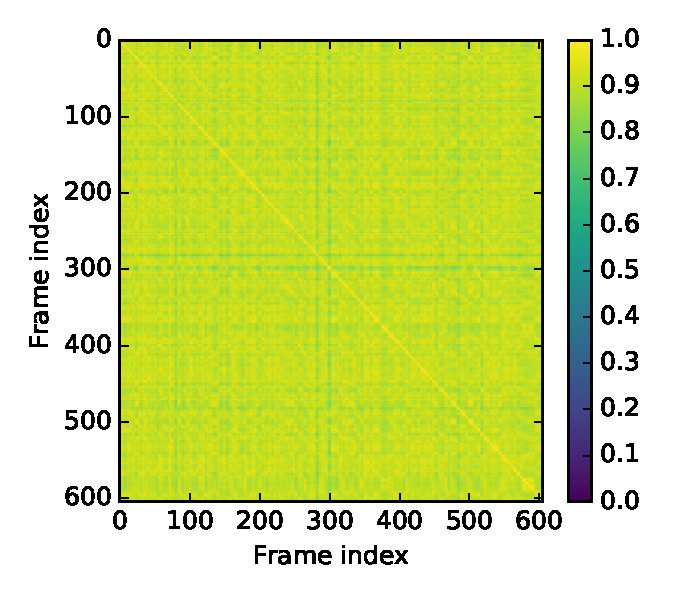
\includegraphics[width=.48\textwidth]{img/ML/mfcc_Down}\label{fig:ML:SSM_mfcc_Down}} \hfil
      \subfloat[Self-Similarity Matrix computed from the MFCC representation of \textit{Orinoco Flow}]{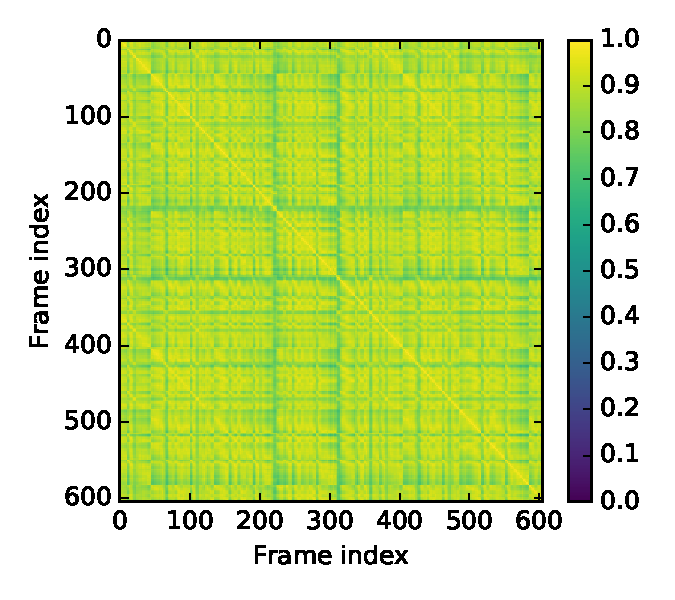
\includegraphics[width=.48\textwidth]{img/ML/mfcc_Henya}\label{fig:ML:SSM_mfcc_Henya}}
        \caption{Examples of Self-Similarity Matrices from MFCC representation}
        \label{fig:ML:SSMs_mfcc}         
\end{figure}

\subsection{Self-Similarity and Self-Distance Matrices}\label{sec:ML:self}
During the design of the linking function, it is often useful to compute the distance among pairs of samples from the input data. %In the case of the signal domain, we usually compute the distance between the representation of different songs, to estimate the similarity between them. 
Several approaches for MSA requires to estimate the inner-song similarity by computing the distance among pairs of frames' representation within the same sample, i.e., the \textit{self-similarity} matrix (SSM).

Given a song representation $\mathbf{S}$ composed of $F$ frame representations $\mathbf{s}_1,..., \mathbf{s}_F$ and a generic distance function $d: \mathbb{R}^{M} \times \mathbb{R}^{M} \rightarrowtail \mathbb{R}$, a \textit{self-distance} matrix is computed as:
\begin{equation}
\mathbf{D}=[d(\mathbf{s}_{i}, \mathbf{s}_{j})] \quad \forall i,j= 1,...,F,
\end{equation}
with $\mathbf{D} \in \mathbb{R}^{F \times F}$. 

The self-similarity matrix is the opposite of the self-distance matrix and it is computed as 
\begin{equation}
\mathbf{M}=1-\tilde{\mathbf{D}},
\end{equation}
where $\tilde{\mathbf{D}}$ is the normalized self-distance matrix. 

The self-similarity and the normalized self-distance matrix carry the same information: the former assigns higher values to closer samples, while the latter assigns higher values to the samples that are far apart. For this reason, sometimes the self-distance matrix is used as a representation of the (inverse) self-similarity.

Depending on the song, on the extracted feature and on the distance function that are used, the SSMs can remarkably vary, hence we can infer different insight on the inner organization of the songs. In Figures \ref{fig:ML:SSMs_mfcc} and \ref{fig:ML:SSMs_chroma}  we show a set of SSMs for the two songs \textit{Orinoco Flow} by the artist Henya and \textit{Down with the Sickness} by the band Disturbed, computed starting from their MFCC (Fig. \ref{fig:ML:SSMs_mfcc}) and chromagram (Fig. \ref{fig:ML:SSMs_chroma}) representations. We see that the matrices generated from the timbral features MFCCs (Figs  \ref{fig:ML:SSM_mfcc_Down} and  \ref{fig:ML:SSM_mfcc_Henya}) exhibit a rather high self-similarity (above $0.7$s) throughout the entire song. Since the timbre is linked to the sound quality of the instruments, we infer that the songs hold the same set of instruments throughout the song, even if some little change of the sound can be seen in \textit{Orinoco Flow} around frames 200 and 300. By visually inspecting the matrices computed from the chromagram representation (Figs  \ref{fig:ML:SSM_chroma_Down} and  \ref{fig:ML:SSM_chroma_Henya}), it is clear that \textit{Orinoco Flow} presents two main musical patterns, which result in a checkerboard-like matrix, while \textit{Down with the Sickness} is more harmonically uniform.

      

\begin{figure}[tb]
        \centering      
 	  \subfloat[Self-Similarity Matrix computed from the chromagram representation of \textit{Down with the Sickness}]{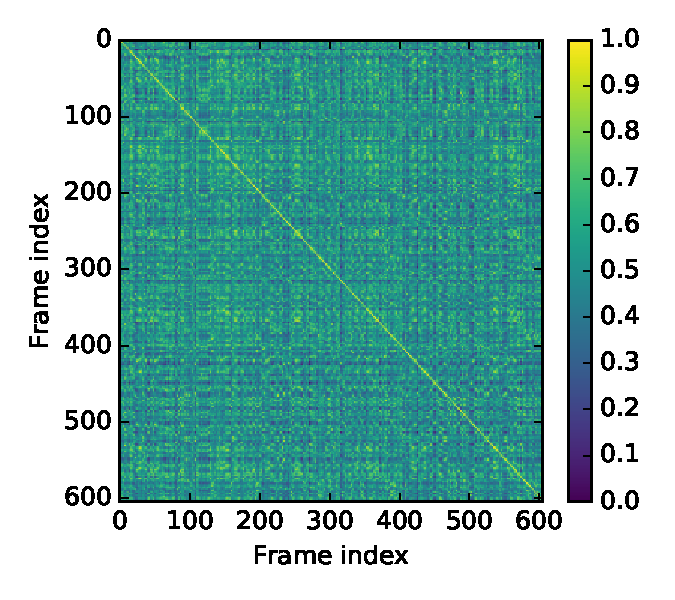
\includegraphics[width=.48\textwidth]{img/ML/chroma_Down}\label{fig:ML:SSM_chroma_Down}} \hfil
      \subfloat[Self-Similarity Matrix computed from the chromagram representation of \textit{Orinoco Flow}]{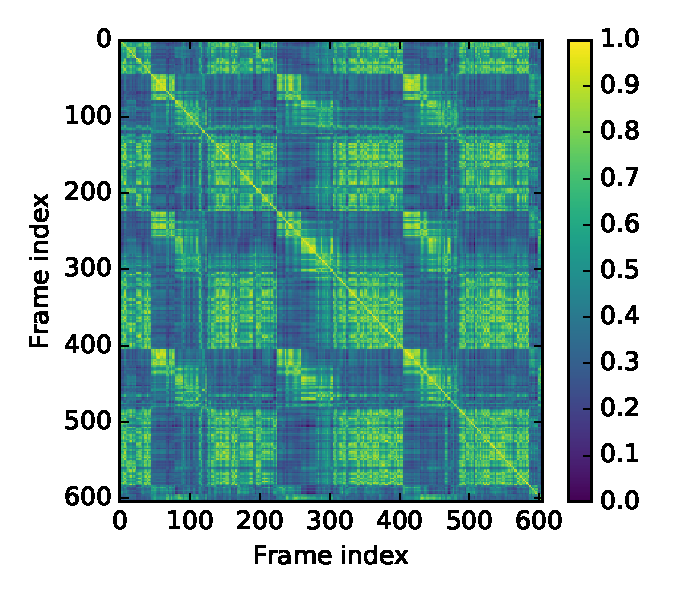
\includegraphics[width=.48\textwidth]{img/ML/chroma_Henya}\label{fig:ML:SSM_chroma_Henya}}
      \caption{Examples of Self Similarity Matrices computed from chromagram representation}
      \label{fig:ML:SSMs_chroma}         
\end{figure}

%While the SSMs are especially used in the context of MSA, the information they provide can be useful for a number of other tasks. In Chapter \ref{Chap:HLFs}, for example, we will compute the SSMs for the data drawn from a dataset for the semantic domain, in order to infer semantic similarity among descriptors.


\subsection{Music Structure Analysis techniques}\label{sec:ML:MSA}
For the Music Structure Analysis (MSA), it is known that the relation between the signal and semantic domains involves the homogeneity of some properties of the musical content or the repetition of musical patterns. This has allowed the MIR community to develop several rule-based techniques to automatically extract the music structure of a song. In this Section we provide an overview of the techniques we use in Chapter \ref{Chap:MSA}.% to address a problem in the context of MSA. Most techniques use a self-similarity or self-distance representation of the songs as presented in previous Section \ref{sec:ML:self}.

The MSA concerns the segmentation of a song into semantically meaningful segments named \textit{sections}, that represents the high-level structural composition of a song, such as \textit{verses}, \textit{chords}, \textit{bridges}, and so on. The MSA involves a first step where the boundaries between sections are detected, and a second step where retrieved sections are grouped together with regard to their role into the song. A more comprehensive discussion on the semantics of the music structure is provided in Chapter \ref{Chap:HLFs}.

One of the first and most popular MSA techniques was proposed by \cite{foote2000automatic}. The basic idea is to extract a curve from the self-similarity matrix that indicates where some novel content appears, and find the peaks of such \textit{novelty curve} to detect the boundaries among sections of the structure. More specifically, the novelty curve is computed by applying a checkerboard filter over the diagonal of the self similarity matrix. The application of the checkerboard filter spots the difference between two consecutive blocks of the self-similarity matrix. It is possible to tune the size of the kernel in order to have a smoother or sharper novelty function and hence be able to detect the boundaries at different time scales, i.e., at different hierarchical levels. 

In \cite{NietoCNMF}, a method based on the factorization of the self-similarity matrix  is proposed. Specifically, it employs a Convex Non-Negative Matrix Factorization (C-NMF) that has some useful properties. The non-negative constraint makes the factorization able to extract a representation of the self-similarity matrix as a sum of components, where the components are called the \textit{basis} of the matrix and the sum is defined by the \textit{activations}. The C-NMF adds the convexity constraint on the basis of the factorization, which must be drawn from the self-similarity itself. Consequently, the C-NMF technique factorizes the self-similarity matrix into a set of components, that represent the sections of the song's structure.

The self-similarity matrix contains the information on the similarity between frames within a song. This information can also be modeled as a graph, where the nodes are represented by the frames of the songs and the edges between nodes are represented by the similarity or the distance between the frames. 

The technique developed by \cite{jensen2005causal} exploits the graph representation to detect the boundaries between sections as the minimum path of the graph from the first to the last frame. The value of the edge between the $i$-th and the $j$-th frame is computed as the sum of the components in the sub-matrix between the $i$-th and the $j$-th rows and columns of the self-distance matrix. The values of the edges are then regularized by the time-distance of the frame (i.e., $j-i+1$) and an offset $\alpha$ is added to model the cost of creating a new segment. The nodes in the shortest path of the obtained graph detect the boundaries between sections. The parameter $\alpha$ defines how much is convenient to create a new segment, so tuning $\alpha$ help to obtain a segmentation at different levels.

The graph representation is also used by \cite{mcfee2014} to apply spectral clustering techniques, which aim at partitioning a graph into different subgraphs by cutting the low-value edges.
As in \cite{jensen2005causal}, this algorithm processes a graph representation of the self-similarity matrix in order to apply graph techniques and find a partition that reflects the musical structure of the song. In particular, the graph is computed from a binary recurrence matrix, i.e., a matrix $ \mathbf{R} \in \{0,1\}^{F \times F}$, where each element $ \mathbf{R}(i,j)$ is equal to 1 if the feature representation of the $i$-th and $j$-th frame are mutually nearest neighbors and to 0 otherwise. This approach leads to detect the boundaries of two different sections as the split of the graph between consecutive frames with a higher distance.

Finally, the algorithm proposed in \cite{Serra2014} uses a different representation of the input, by defining a set of so-called \textit{structure features} (SF) to perform the boundary detection. The structure features are built by wrapping different samples in the same row, i.e., the $f$-th row of the SF matrix representation is made by considering the previous and next frames with respect to the $f$-th frame. This helps in incorporating some time-information in the structure, making it more robust to short-time variations. The SF matrix is then smoothed with a Gaussian Kernel and a novelty function is computed between consecutive rows. The boundaries between sections are detected as peaks in the novelty curve as made by \cite{foote2000automatic}.

%In Chapter \ref{Chap:MSA} we will present a research study of ours that makes use of the abovementioned techniques to address an application scenario of MSA.

\section{Machine Learning Techniques}\label{sec:ML:models}
Machine learning techniques have been effectively used in MIR literature to model the human perception of the music. The machine learning models involves the retrieving of patterns in the input data (unsupervised models) or the prediction of an outcome from the representation of the input (supervised models). In this section we present an overview of the machine learning techniques used as a linking function for a number of scenarios.

In Section \ref{sec:ML:clust} we first present a set of clustering techniques, which aims at retrieving some patterns in the input data by grouping together samples that share some properties. Commonly, the algorithms for clustering are used as an unsupervised approach, so they do not have any clue on the patterns they are expected to retrieve. In some cases, however, the clustering techniques are adapted to embody some prior knowledge as constraints (semi-supervised techniques). The clustering techniques rely on a metric of distance between samples, which is commonly a linear metric such as the Euclidean distance. In some cases, however, it might be helpful to use a different metric that makes some pattern between samples explicit. In Section \ref{sec:ML:dist} we present the distance learning techniques, that aim at defining a metric of distance from a set of prior constraints on the data. Finally, in Sections \ref{sec:ML:classifiers} and \ref{sec:ML:semantics} we present a set of supervised machine learning techniques for the prediction of a categorical or dimensional outcome, respectively. The supervised techniques are able to learn a predictive model from a set of labeled data. It is worth remembering that, as discussed in \ref{sec:ML:data}, for supervised techniques it is common to train the model with a subset of the data (the training set) and evaluate the model with the rest of the data (the test set). Such evaluation is referred to as test error, while the evaluation computed over the training set is referred to as training error. 

In this section we follow the formalization introduced in Section \ref{sec:ML:data} for the design of the linking function. Given the dataset $\mathcal{X}=\{x_1,...,x_N\}$, we refer to the relative counterpart in the codomain of the problem as the dataset $\mathcal{Y}=\{y_1,...,y_N\}$ and to the whole possibly annotated dataset as $\mathcal{D}=\{(x_1, y_1),...,(x_N, y_N)\}$. The generic codomain image $y_i$ receive several formalizations depending on the addressed problem and the designed linking function. %we are not using the bold font because the outcome might not be a vector. 
%In the following Sections we will present the formalization of the codomain for the specific use cases.


\subsection{Unsupervised and Semi-Supervised Clustering}\label{sec:ML:clust}
A clustering method is a usually unsupervised technique that aims at grouping a dataset of samples based on a given definition of distance or similarity \cite{PAMI}. Several techniques have been proposed in the literature, aiming at grouping samples with different shapes or by exploiting various principles \cite{jain1999data}. Since a comprehensive discussion is beyond the scope of our work, we present here the approaches we use for our work.

The K-Means \cite{macqueen1967some} algorithm is one of the most widely used unsupervised clustering technique. Given an initial set of $K$ candidates for centroids, the algorithm involves two steps that are iterated until convergence: 
\begin{enumerate}
	\item each sample is assigned to the closest centroid, i.e., to the correspondent cluster;
	\item the position of the centroids are updated in order to represent the actual centroids of the samples in their cluster.
\end{enumerate}
The K-Means algorithm requires the user to select the desired number of clusters $K$, which is often not known in advance.  Moreover, the choice of the initial set of centroids is crucial in the resulting clusters, so it needs to be accurate. 

The X-Means algorithm is proposed by \cite{Pelleg2000} to overcome the former limitation. The algorithm runs the K-means algorithm several times, for each $K=K_{min},...,K_{max}$, and chooses the $K$ and clustering that exhibits the higher quality measure. The authors propose two measures: the Bayesian Information Criterion (BIC) and the Akaike Information Criterion (AIC) measures.

The latter limitation is usually addressed by choosing a random set of samples as the initial candidates for the centroids, and running the K-means algorithm for a number of times, each time with a different random set of candidates, in order to choose the set that best describes the data for some objective metrics \cite{PAMI}. An algorithm for the selection of the initial set of candidates is also proposed in \cite{Arthur2007}.

The K-means algorithm is especially effective in retrieving clusters with a globular shape \cite{PAMI} (i.e., with similar variance in all the dimensions), since each cluster aggregates the data around a centroid. In order to retrieve clusters with a different shape, other techniques might be more effective. 

The Agglomerative Hierarchical Clustering \cite{sibson1973slink} (AHC) follows a hierarchical bottom-up approach to build the clusters. At first, each sample is assigned to a different clusters, so we have $M=N$ clusters. Iteratively, the two closest clusters in the set merge together, leading to $M-1$ total clusters. The clusters keep merging until the desired final number of clusters $K$ is reached. %The algorithm can lead to different 
The final clustering results depend on which metric is used to estimate the distance between two clusters. The most common metrics are \cite{Tan2005}:
\begin{itemize}
	\item the \textit{complete-linkage clustering}, which considers the maximum distance between the samples in the two clusters; 
	\item the \textit{single-linkage clustering}, which considers the minimum distance between the samples in the two clusters; 
	\item the \textit{average-linkage clustering}, which considers the average distance between the samples in the two clusters; 
	\item the \textit{centroid-linkage clustering}, which considers the distance between the centroids of the two clusters.
\end{itemize}

In Section \ref{sec:ML:MSA} we reviewed the Spectral Clustering and Non-Negative Matrix Factorization (NMF) for the MSA task. The two approaches have originally been employed for clustering of data. 

The Spectral Clustering \cite{shi2000normalized} (SC) technique processes a graph built from the input data, with the nodes given by the samples and the edges defined by the distances between them. The SC technique looks for the lowest cost partition of the graph, by evaluating  the \textit{normalized cut}, which is a measure of the dissociation between two cluster that considers both the weights of the edges between the two groups and the weights of the edges of each group with respect to the overall graph. This approach ensures that the final cut is made between well separated and well balanced clusters. The basic SC algorithm cuts a graph, i.e., a dataset, into two groups, and can be used recursively to obtain $K$ clusters. In \cite{shi2000normalized} the authors propose an approach to generalize the algorithm to cut the graph into $K$ subgroups.

In \cite{xu2003document} the authors propose an algorithm for clustering based on a Non-Negative Matrix Factorization. The NMF is used to decompose a matrix into a positive sum of the main components, which, in this case, represent the main clusters. More specifically, this approach processes the input data representation $\mathbf{X}$ in order to compute two matrices $\mathbf{U}$ and $\mathbf{V}$ representing the cluster centroids and the clusters' association respectively.

The clustering of samples is a commonly unsupervised task. However, some algorithms are adapted to be trained in a semi-supervised fashion, in order to consider some desiderata on the final clustering, by providing a set of constraints. Two sets of constraints are defined, the Must-Link $ML$ and Cannot-Link $CL$, that collect the samples that must be or must be not grouped together, respectively.

In \cite{chen2008} the authors propose a Semi-Supervised approach for the algorithm based on Non-Negative Matrix Factorization (SS-NMF). This approach uses the distance matrix $\mathbf{D}$ computed from the sample of the input data $\mathbf{X}$ instead of the data itself. The distance matrix is processed in order to include the information from the $ML$ and $CL$ sets as  
\begin{equation}
\hat{\mathbf{D}}=[\mathbf{D}(i,j) - \zeta_{i,j} + \vartheta_{i,j}] 
\label{eq:ML:constr}
\end{equation}
where $\zeta_{i,j}> 0$ if $(i,j)$ is in the $ML$ set and $\vartheta_{i,j}> 0$ if $(i,j)$ is in the $CL$ set. The Equation \ref{eq:ML:constr} makes the samples in the $ML$ set closer and the samples in the $CL$ set further apart. The values of $\zeta_{i,j}$ and $\vartheta_{i,j}$ can be determined from the weight of the correspondent constraints, or set to a standard constant value.

The approach defined in \cite{chen2008} can be used also for AHC and SC algorithms, since they also compute the clusters from a distance matrix between the samples. Some modifications of K-means are also proposed to include the constraints and make the algorithm semi-supervised \cite{Basu2002}.

In \cite{peng2007} the authors propose the use of a semi-supervised variant of the K-Means clustering algorithm to group together tracks from a music library according to some criterion, and they apply the technique for grouping tracks by similar artists.
In \cite{dieleman15} the authors apply the K-Means to cluster the features learned with a neural network and use the obtained centroids as a more compact representation of the features.


\subsection{Distance Learning techniques}\label{sec:ML:dist}
Several rule-based and machine learning techniques need to estimate the distance among samples, e.g., the clustering techniques described in the previous Section \ref{sec:ML:clust}. For this scope, we use standard distance metrics as well as kernel metrics. 

However for some problems we need to shape the distance metric in order to reflect some property of the similarity. \textit{Distance Learning techniques} are designed to learn a representation of the distance by exploring which features or relation among them are more relevant for a specific scope. 

Two of the most common distances are: the Euclidean distance
\begin{equation}
d(\mathbf{x}_i,\mathbf{x}_j)=\sqrt{(\mathbf{x}_i-\mathbf{x}_j)\T (\mathbf{x}_i-\mathbf{x}_j)};
\end{equation}
and the Cosine distance
\begin{equation}
d(\mathbf{x}_i,\mathbf{x}_j)=1- \frac{\mathbf{x}_i\T \mathbf{x}_j}{||\mathbf{x}_i||\; ||\mathbf{x}_j||},
\end{equation}
that assign the same importance to the different components of the samples.

We include a weighting of the components by defining a diagonal matrix $\mathbf{A}$ and computing the \textit{Mahalanobis distance}:
\begin{equation}
\begin{split}
d(\mathbf{x}_i,\mathbf{x}_j) & =  ||(\mathbf{x}_i-\mathbf{x}_j)||_\mathbf{A} = \\
& =\sqrt{(\mathbf{x}_i-\mathbf{x}_j)\T \mathbf{A} (\mathbf{x}_i-\mathbf{x}_j)};
\end{split}
\label{eq:ML:mahalanobis}  
\end{equation}
where $\mathbf{A} \in \mathbb{R}^{M \times M}$ is the \textit{Mahalanobis matrix} \cite{xing2003distance}. Each element in the diagonal $\mathbf{A}(m,m)$ indicates the degree of relevance that is assigned to the $m$-th component. The Euclidean distance can be seen as a specific case where $\mathbf{A}=\mathbf{I}$ is the identity matrix.

For some problems, weighting the relevance of the single components is not sufficient, and we need to compute a distance metric that takes into account the inter-correlation among the components. In order to do so, we use a full symmetric matrix $\mathbf{A}$, where each element $\mathbf{A}(i,j)$ that is not in the diagonal models the interaction between the $i$-th and the $j$-th component \cite{xing2003distance}.

The Mahalanobis distance can also be seen as a traditional Euclidean distance computed over a transformation of the input space. In fact, the Equation \ref{eq:ML:mahalanobis} can be also written as:
\begin{equation}
d(\mathbf{x}_i,\mathbf{x}_j)=\sqrt{(\mathbf{L}\mathbf{x}_i-\mathbf{L}\mathbf{x}_j)\T (\mathbf{L}\mathbf{x}_i-\mathbf{L}\mathbf{x}_j)},
\end{equation}
where $\mathbf{L}\T \mathbf{L}=\mathbf{A}$, provided that $\mathbf{A}$ is positive semi-definite. The matrix $\mathbf{L}$ defines the subspace where the Mahalanobis distance is applied. The Distance Learning techniques aim at finding the Mahalanobis matrix $\mathbf{A}$ or the subspace $\mathbf{L}$ that best shape the distance metric. As in the kernel expansion example, we can use $\mathbf{L}$ to map the input space in a new space and compute the Euclidean distance over the new, learned space.

In order to learn a distance metric, we need some example data that explains the desiderata of the metric. This is commonly done by defining a set of \textit{Must-Link} (ML) and \textit{Cannot-Link} (CL) constraints \cite{xing2003distance}, as also discussed in Section \ref{sec:ML:clust} for semi-supervised clustering techniques. 


\begin{figure}[tb]
	\centering
	\subfloat[Generic distribution of data for the example on Distance Learning]{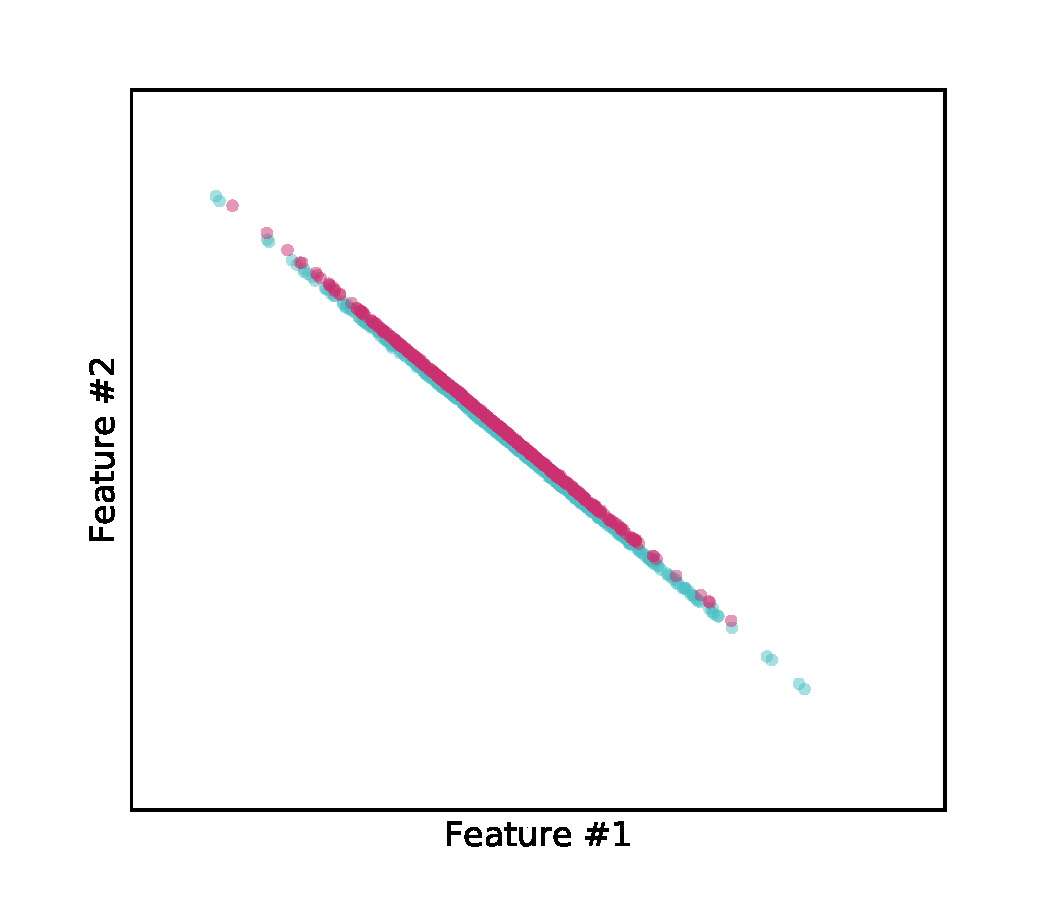
\includegraphics[width=.48\textwidth]{img/ML/ML_DL_original}\label{fig:ML:DL_original}} \hfil
	\subfloat[Visualization of the constraints used for the example]{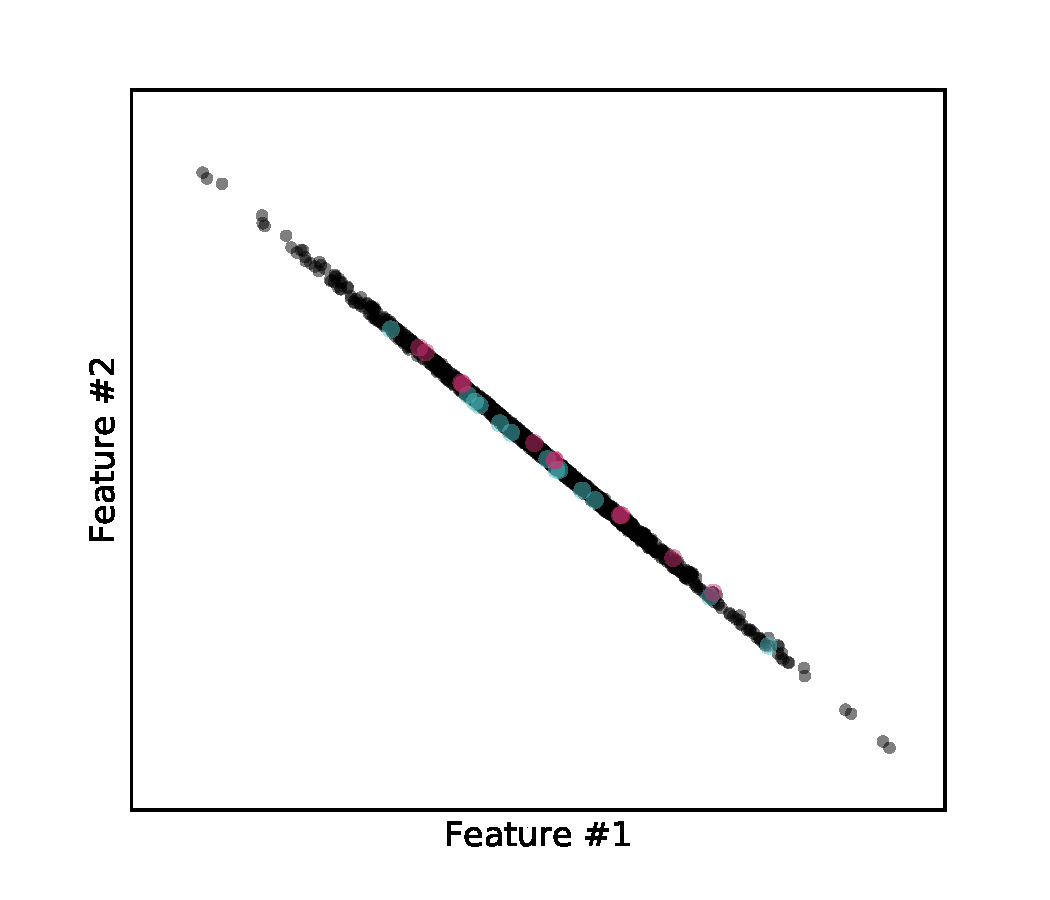
\includegraphics[width=.48\textwidth]{img/ML/ML_DL_constraints}\label{fig:ML:DL_constraints}}
	\caption{Generic distribution and constraints used for the example on distance learning}
	\label{fig:ML:DL_OC}         
\end{figure}

In Figure \ref{fig:ML:DL_OC} we present a visualization for an example of the distance learning techniques. Let us suppose to have data from two distributions, as shown in Figure \ref{fig:ML:DL_original}. We want to learn a distance metric able to assign high distances to samples in different distributions and low distances for samples in the same distributions. However, in our example scenario, we only rely on a few constraints shown in Figure \ref{fig:ML:DL_constraints}. Nevertheless, distance learning techniques are able to exploit the information provided by the constraints to learn a distance metric or a transformation of the space. In this work we use three techniques for distance learning. 

The first technique computes the Mahalanobis matrix by iteratively following some steps, and is therefore named \textit{Iterative Projection} \cite{xing2003distance} (IP). It defines a function $g(\mathbf{A})$ that estimates the sum of the Mahalanobis distances between the samples in the set $CL$ and a function $f(\mathbf{A})$ that estimates the sum of the Mahalanobis distances between the samples in the set $ML$. The goal is to maximize $g(\mathbf{A})$ and to minimize $f(\mathbf{A})$. The IP algorithm iteratively estimates the gradient of $g(\mathbf{A})$ with respect to $f(\mathbf{A})$ and makes use of a gradient ascent algorithm to converge to the optimal Mahalanobis matrix.

The second technique is named \textit{Relevant Components Analysis}\cite{bar2003learning} (RCA), because it performs an analysis of the relevance of each component for the computation of the distance. The RCA algorithm aims at assigning large weights to relevant dimensions and low weights to irrelevant ones. The relevance of the components are estimated within \textit{chunklets}, which are subsets of the data from the ML set. The Mahalanobis matrix is computed as the inverse of the covariance matrix of samples within the chunklets. This procedure reduces the relevance of the interaction of the components that exhibit a lower covariance.

The third technique is described in \cite{goldberger2004neighbourhood} and is named \textit{Neighborhood Components Analysis} (NCA), since it follows a nearest neighborhood approach. Such approach selects for each sample the $K$ nearest samples and define special properties for the samples that are mutual nearest neighborhood Specifically, the NCA algorithm aims at maximizing $f(\mathbf{A})$ the number of mutual nearest neighborhood samples among those defined in the $ML$ set. In order to do so, it applies a gradient ascent over $f(\mathbf{A})$ with respect to $\mathbf{A}$.

\begin{figure}[tb]
	\centering
	\subfloat[IP applied to the example ]{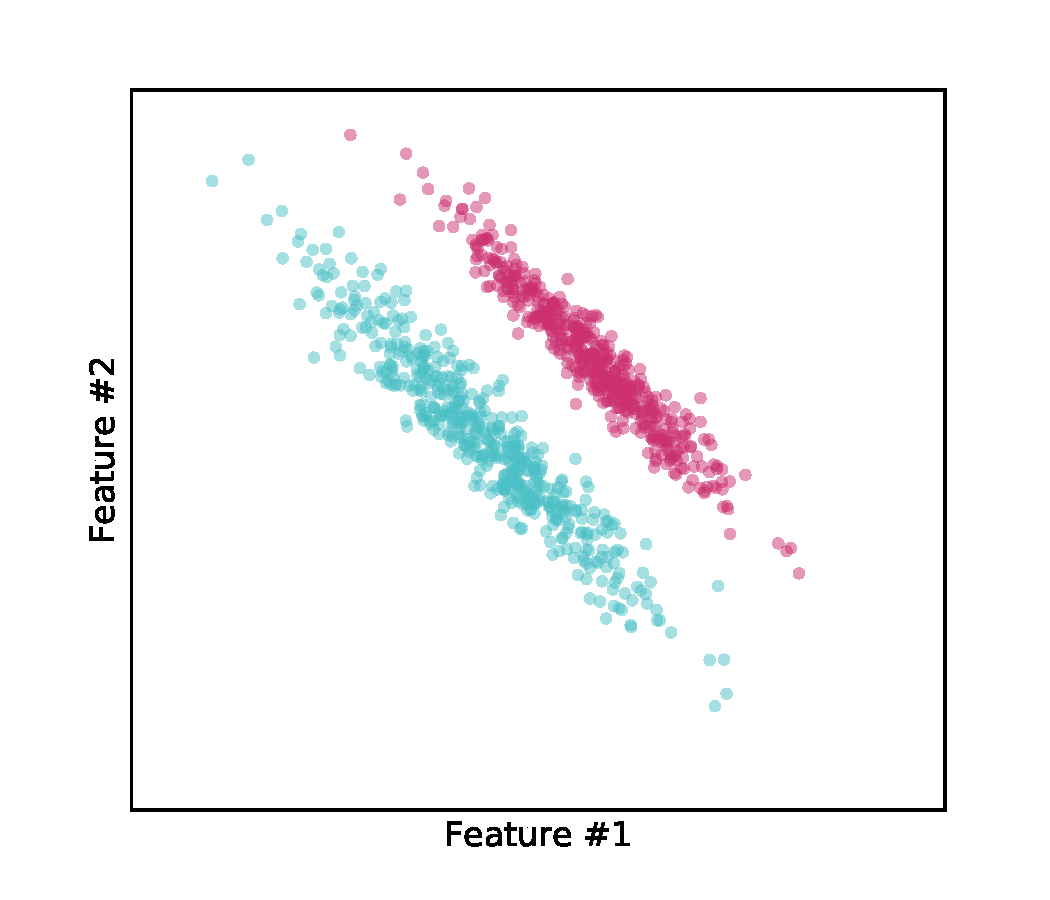
\includegraphics[width=.33\textwidth]{img/ML/ML_DL_IP}\label{fig:ML:DL_IP}} \hfil
	\subfloat[RCA applied to the example ]{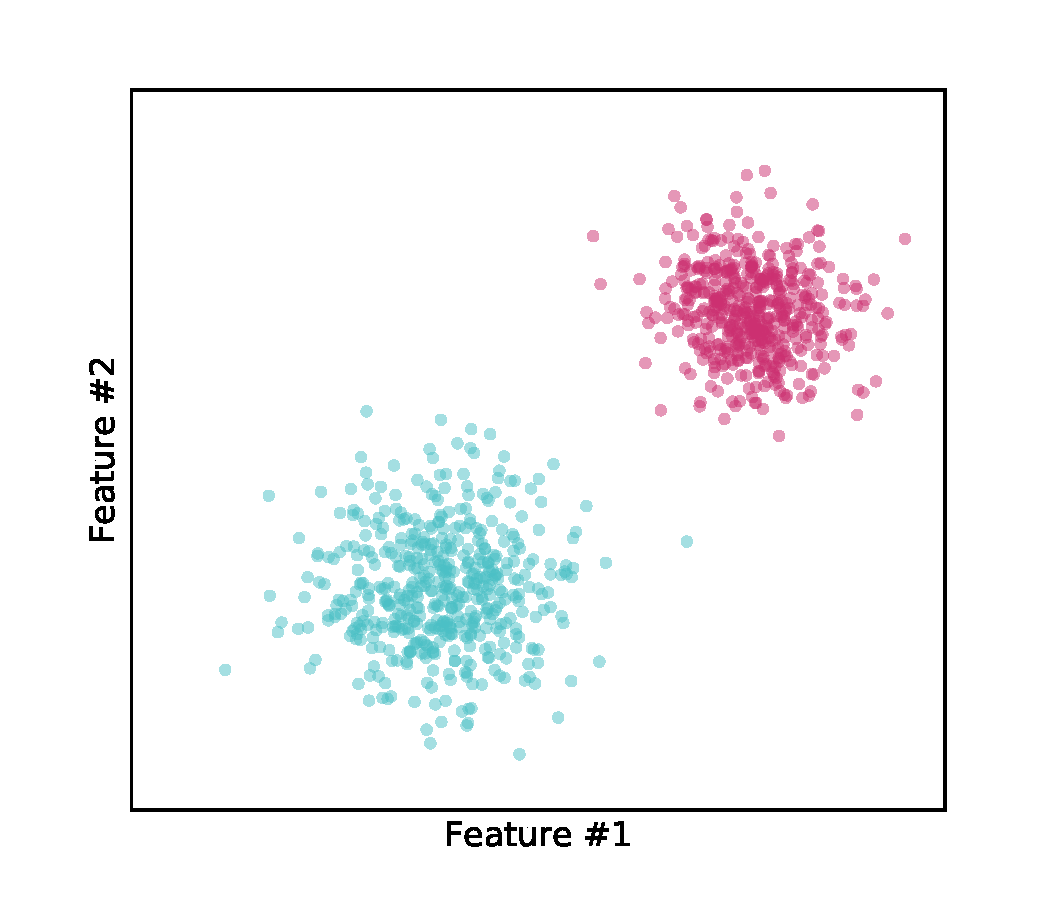
\includegraphics[width=.33\textwidth]{img/ML/ML_DL_RCA}\label{fig:ML:DL_RCA}} \hfil		
	\subfloat[NCA applied to the example ]{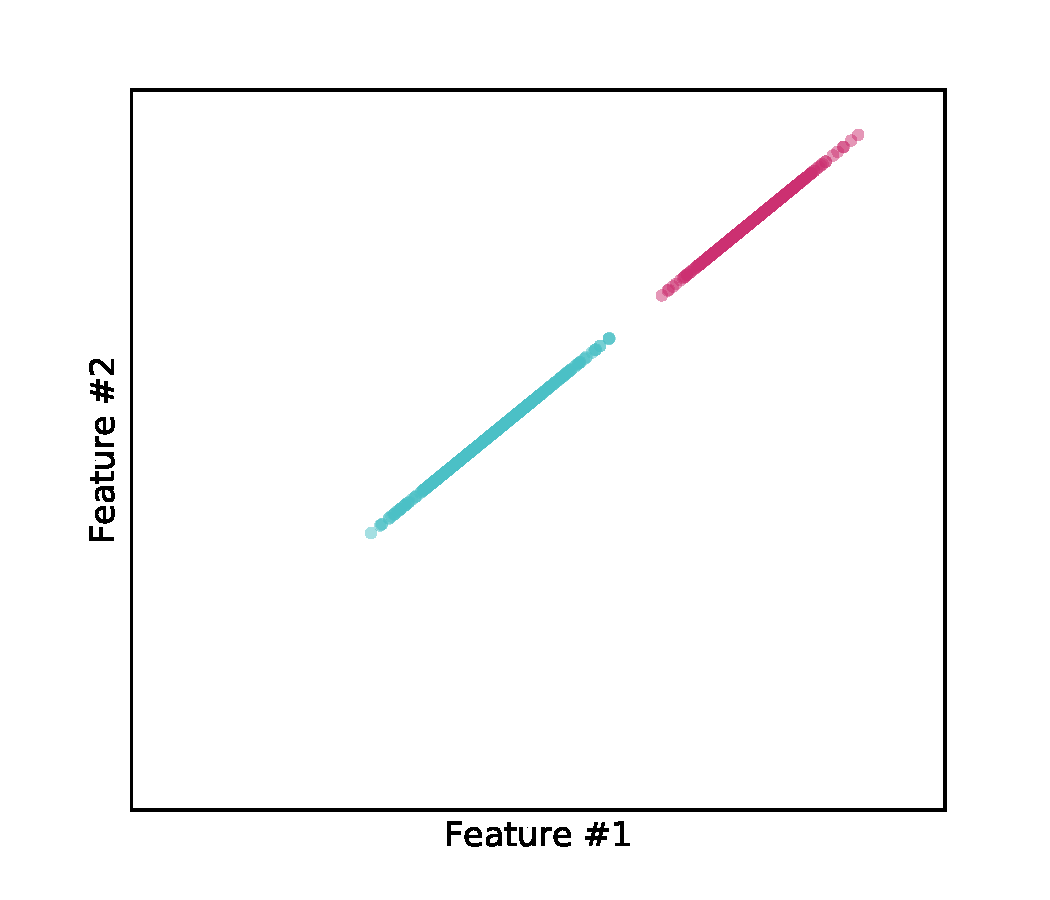
\includegraphics[width=.33\textwidth]{img/ML/ML_DL_NCA}\label{fig:ML:DL_NCA}} 
	\caption{Examples of the application of different distance learning techniques}
	\label{fig:ML:DL_IPNCARCA}         
\end{figure}

In Figure \ref{fig:ML:DL_IPNCARCA} we show the behavior of the three techniques for the example provided in Figure \ref{fig:ML:DL_OC}. We compute the transformation matrix $\mathbf{L}$ with the techniques and we apply them to the original distribution of data.  The IP algorithm shown in Fig. \ref{fig:ML:DL_IP}, is able to well separate the two distributions. However, we notice that the centroids of the distribution are closer with each other than with the samples at the edge of their distribution. The same drawback appears when NCA technique is applied (Fig. \ref{fig:ML:DL_NCA}), where the shape of the distribution is also somehow preserved. In this example, the best performance is provided by the RCA technique, in Fig. \ref{fig:ML:DL_RCA}, which manages to well separate the two distributions and also reduce the distance between samples in the same distribution. It is worth noting that we can not draw conclusions on the effectiveness of the techniques from this example alone. Nevertheless, we observe that all the techniques are able to detect and separate the two distributions from a set of few constraints.

\subsection{Machine Learning techniques for classification}\label{sec:ML:classifiers}
In the machine learning literature, a classifier is defined as a model that aims at predicting a categorical outcome from the input data \cite{PAMI}. The classifiers can be used whenever the codomain of the problem is formalized with discrete values. In this Section we provide a review for two main approaches for classification: the linear classifier and the Support Vector Machine (SVM).


%The music classification (Section \ref{sec:HLFs:class}) and categorical annotations (Section \ref{sec:HLFs:anns}) have in common the basic approach to formalize the semantic codomain, i.e., to predict whether a certain HLF can be used to describe a certain music piece. In the former scenario, a set of labels can be defined to fully define the semantic codomain. In the latter scenario a set of descriptors is defined, and each descriptor performs a partition of the codomain into the presence or absence of the related characteristics. Both problems can be addressed by modeling the linking function as a classifier. 

%If we aim at classifying a certain frame $\iota$ into $P$ non-overlapping labels, we can model the desired output as a matrix $\mathbf{Y} \in \{-1,+1\}^{F\times P}$ where each row $\mathbf{y}_\iota \in \mathbb{R}^{1 \times P}$ has a value equal to $+1$ in the $p$-th component relative to the label of the $\iota$-th sample and $-1$ otherwise. If we aim at annotating the frame within a set of $P$ descriptors instead, we set $\mathbf{y}_\iota^{(p)}=+1$ to indicate the presence of the $p$-th HLF in the description of the $\iota$-th frame, and $\mathbf{y}_\iota^{(p)}=$ to indicate its absence. 

The linear classifier is the most simple classifier, and it assumes that the outcome of a model can be predicted as a linear combination of the input components. Let us consider the simplest case, a two-class classifier where each outcome is formalized as $y_i=\{-1,+1\}$ depending on which class it belongs to. The linear classifier predicts the outcome as: 
\begin{equation}
\hat{\mathbf{Y}}=\tilde{\mathbf{X}} \mathbf{b},
\label{eq:ML:linClassPred}
\end{equation}
where $\tilde{\mathbf{X}}$ is the regularized representation of the domain, $\mathbf{b} \in \mathbb{R}^{M}$ is the vector of parameters for the classifier and $\hat{\mathbf{Y}}$ are the predicted values. 

The linear classifier is trained in order to learn the vector $\mathbf{b}$, i.e., the weights of the linear combination. More specifically, each component $\mathbf{b}_m$ represents the weighting for the $m$-th input component. The predicted output $\hat{\mathbf{Y}}$ is actually continuous and needs to be discretized by applying the sign function component-wise over the vector $\hat{\mathbf{Y}}$, in order to estimate the final class.

The learning of the parameters for the linear classifier is trivial, since it only involves the multiplication of the pseudo-inverse of the input matrix $\tilde{\mathbf{X}}$ with the expected outcome $\mathbf{Y}$ :
\begin{equation}
\mathbf{b}=(\tilde{\mathbf{X}}\T \tilde{\mathbf{X}})^{-1}  \tilde{\mathbf{X}}\T  \mathbf{Y}.
\label{eq:ML:linClass}
\end{equation}

The linear classifier can be generalized in the number of classes and in the number of total classifiers. If we need to estimate a set of $P$ 2-class classifiers for the input data, i.e., $ \mathbf{y}_i \in \{-1,+1\}^P$, we generalize the model by simply considering a matrix of
output data $\mathbf{Y}$  and predicted output data $\hat{\mathbf{Y}}$, both with $N$ rows (the number of samples, and $P$ columns (the number of classifiers). By substituting the matrix  $\mathbf{Y}$  in Equation \ref{eq:ML:linClass}, we obtain the matrix of parameters $\mathbf{B}\in\mathbb{R}^{M \times P}$, where each column $\mathbf{B}^{(p)}$ takes the role of the vector of parameters $\mathbf{b}$. The matrix is used in Equation \ref{eq:ML:linClassPred}, with the same discretization of $\hat{\mathbf{Y}}$ performed column-wise.

If, instead, we need to train a $P$-class classifiers, we still use a formalization of the output data such that $ \mathbf{y}_i=\{-1,+1\}^P$, where $ \mathbf{y}_i^{(p)}=+1$ if $x_i$ belongs to the $p$-th class and $ \mathbf{y}_i^{(p)}=-1$ otherwise. This approach is referred to as one-versus-all \cite{Manning2008}. The same Equations \ref{eq:ML:linClassPred} and \ref{eq:ML:linClassPred} hold also for this case, while the interpretation of the matrix of parameters $\mathbf{B}\in \mathbb{R}^{P \times M}$ is slightly different: each column $\mathbf{B}^{(p)}$, indeed, represents a model specifically trained for the $p$-th class, i.e., it is similar to train $P$ 2-class classifiers, each of them aims at predicting the $p$-th class. The discretization of $\hat{\mathbf{Y}}$ also changes. In this case, we assign each  sample to the class that is predicted with a higher likelihood. In order to do so, we consider each row $\hat{\mathbf{y}}_i$, and we compose a vector with all components equal to $-1$ except for $\hat{\mathbf{y}}_i^{(q)}=+1$ , with $q=\argmax{p} \hat{\mathbf{y}}_i^{(p)}$. 

The linear classifier has a simple geometric interpretation: each vector $\mathbf{b}$ defines a manifold in the input space that is  shaped in order to have high values where the input samples of a certain class are more likely to be distributed and low values where they are not. 

\begin{figure}[tbp]
	\begin{center}
		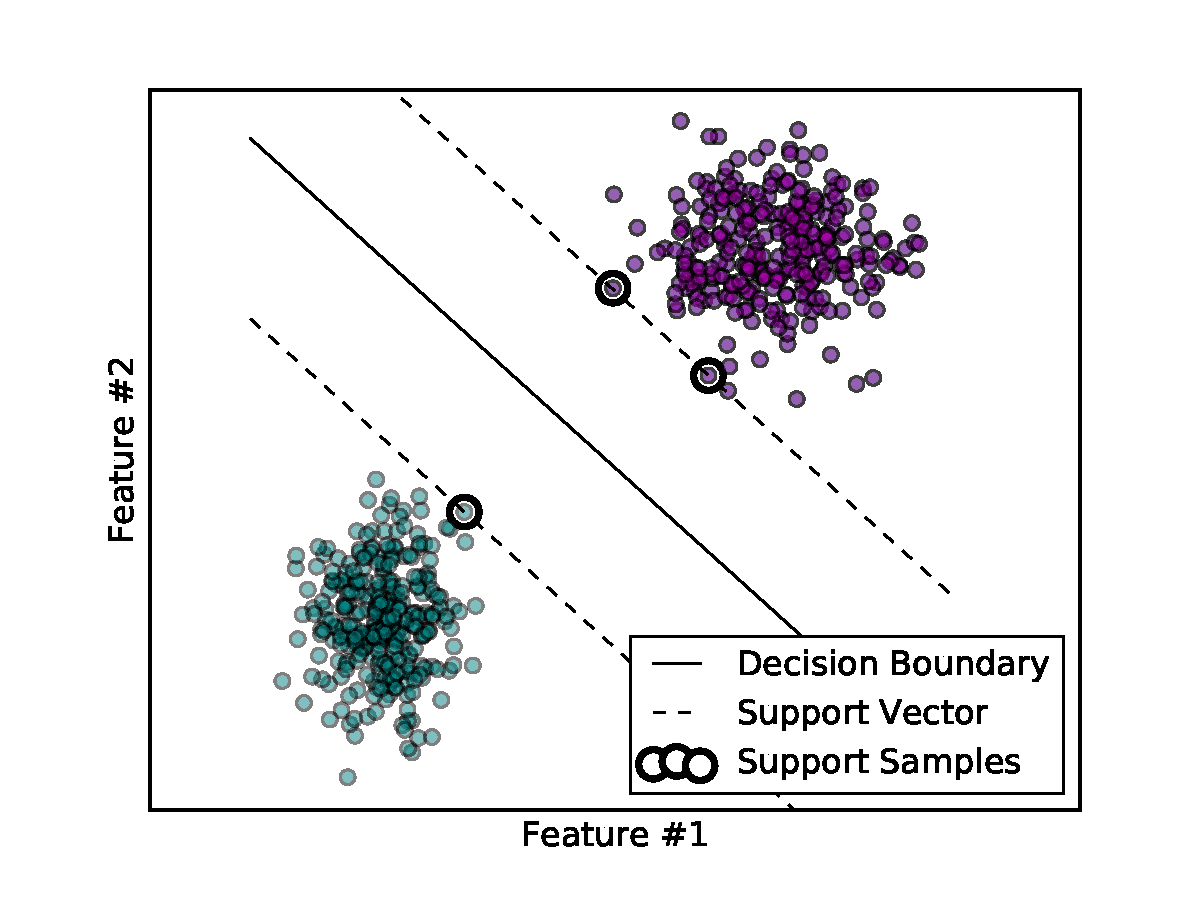
\includegraphics[width=12cm]{img/ML/ML_SVM}
		%\psfig{file=img/ML/logopm.jpg,width=3.5cm}
	\end{center}
	\caption{A graphic representation of the SVM classifier}
	\label{fig:ML:SVM}
\end{figure}

The Support Vector Machine (SVM) classifier follows a different approach, by learning the hyperplane that separates the input data that belong to a certain class from those that do not. The hyperplane is designed in order to have the maximum possible separation between the classes. In order to do so, the SVM technique relies on \textit{support vectors}, that are the vectors that connect the samples of the two classes which are closer to a given hyperplane, i.e., the \textit{support samples}. Maximizing the distance between the hyperplane and the support vectors leads to a better separation between classes. We show a representation of the behavior of SVM in Figure \ref{fig:ML:SVM}.

The SVM is a binary classifier, i.e., it only learns a hyperplane that separates two classes. However, we generalize its behavior using the aforementioned one-versus-all strategy by learning $P$ SVMs, each of which separates the samples that belong to the $p$-th class from those that do not. The final prediction is actually similar to the one for the linear classifier: the label that achieves the higher likelihood is assigned to the sample.

The SVM classification is a simple application of the hyperplane $\mathbf{w}\in \mathbb{R}^{M}$ to the generic frame $\mathbf{x}_i$ such that
\begin{equation}
\hat{y}_i=\text{sign}(\mathbf{w}\T \mathbf{x}_i + b)
\end{equation}
where $y_i$ indicates the predicted output for a generic SVM and $b$ is the intercept of the hyperplane. We learn the manifold by solving the minimization problem:
\begin{equation}
\begin{split}
\min  ||\mathbf{w}||^2\\
\text{subject to  } y_i(\mathbf{w}\T \mathbf{x}_i)\geq 1 \\
\forall i=1,...,N
\end{split}
\label{eq:ML:SVM}
\end{equation}

%The two class problem is usually generalized to multi-class problems by training several SVM classifiers, where each of them classify whether a sample belongs to a certain class and the class that has a higher estimated value is assigned to the sample.

Both the linear and SVM classifiers use a linear combination of the input to design the classification function. However, they can exploit nonlinearity relationship between features by using kernel expansion techniques presented in Section \ref{sec:ML:kernels}. This allows the two classifiers to learn decision surfaces that are nonlinear with respect to the feature space, empowering the predictive power of the models.

%The two classifiers are still linear with respect to the components, but since the components are now a nonlinear transformation of the original input space, it results in a decision function that is nonlinear in the input space.

In this thesis we use classification techniques in Chapter \ref{Chap:Bootleg}, to model a linking function from a representation of the signal domain to a non-overlapping labeling of the semantic domain.


\subsection{Machine Learning techniques for regression}\label{sec:ML:semantics}
Regressors are defined as machine learning techniques that are able to predict an outcome within a continuous range of values. In this section we provide an overview of the regressor techniques we use in our work. We use a similar notation as in Section \ref{sec:ML:classifiers}, with the expected normalized output defined as $\mathbf{Y}\in [0,1]^{N \times P}$.
%, where each column $\mathbb{Y}^{p}$ with $p=1,...,P$ models the $p$-th descriptor.

Similarly to the linear classifier (Section \ref{sec:ML:classifiers}), we can model a regressor as a linear combination of the input components \cite{Sen1990}. The linear regression \cite{PAMI} is based on the same principle of the linear classifier, hence we use the same Equations \ref{eq:ML:linClassPred}, \ref{eq:ML:linClass} to learn the parameters and compute the predicted values, by using the dimensional definition of $\mathbf{Y}$. From a geometric interpretation a linear regression model aims at learning the manifold that minimizes the squared distance between the manifold at a given point (i.e., the predicted value) and the correspondent expected value.

The linear approach is simple but often effective to model the linking function. However, it may also lead to overfitting, i.e., to learn a model that fits too much the training data and it is not general for the real-case scenario. The Ridge Regressor addresses the over-fitting issue by setting a constraint on the sums of the parameters of the linear combination \cite{PAMI}, i.e., on the maximum $||\mathbf{b}||$ in Equation \ref{eq:ML:linClass}. The constraint forces the model to share the predictive power of the weights of the linear combination, hence to focus on the more informative components. This leads to a higher training error, but it often achieves higher performance in the real world scenario. Given the parameter $\lambda$, related to the constraint on the sum of parameters, we train the parameters of the model by computing \cite{PAMI}
\begin{equation}
\mathbf{B}^{ridge}=(\mathbf{X}\T \mathbf{X}+\lambda \mathbf{I})^{-1}  \mathbf{X}\T  \mathbf{Y}.
\label{eq:ML:ridge}
\end{equation}
The constraint on the sum of parameters is a common regularization method also known as \textit{weight decay}.

\begin{figure}[tbp]
	\begin{center}
		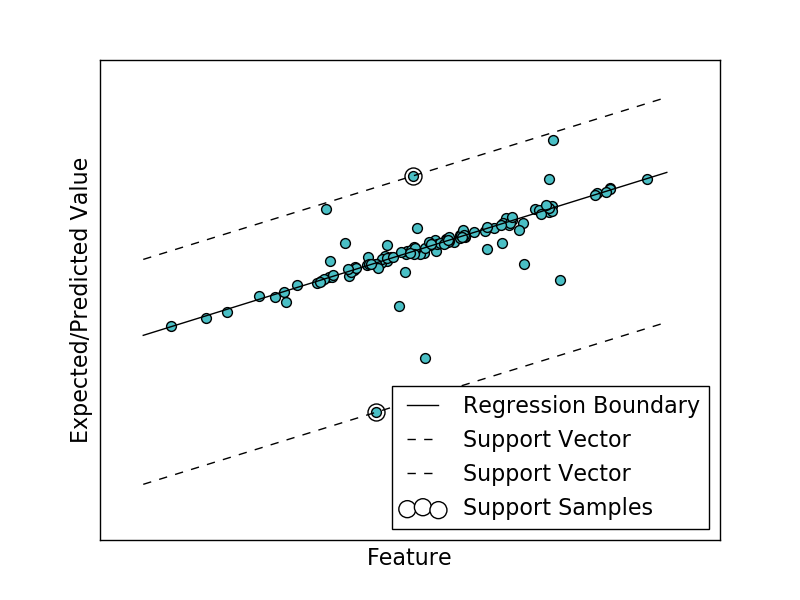
\includegraphics[width=12cm]{img/ML/ML_SVR}
		%\psfig{file=img/ML/logopm.jpg,width=3.5cm}
	\end{center}
	\caption{A graphic representation of the SVR regressor}
	\label{fig:ML:SVR}
\end{figure}

A similar parallelism between linear classifier and regressor also holds for the Support Vector Machine. The support vectors are used to predict a continuous value by using the Support Vector Regression (SVR) model \cite{Rho2009}. While in classification the support vectors are used to find the manifold that maximizes the separation between classes, in the regression problem the support vectors identify the manifold that minimizes the mean squared error of samples, as shown in Figure \ref{fig:ML:SVR}. With respect to the minimization problem of Equation \ref{eq:ML:SVM}, in the SVR we want to minimize
\begin{equation}
\begin{split}
\min  ||\mathbf{w}||^2\\
\text{subject to  } (y_i-\mathbf{w}\T \mathbf{x}_i)^2\leq \epsilon^2 \\
\forall i=1,...,N
\end{split}
\label{eq:ML:SVR}
\end{equation}
where $\epsilon$ is the maximum allowed error.

The linear and ridge regression models are based on the assumption that the output value can be predicted as a (possibly constrained) linear combination of the components. In order to overcome the limitations of the linearity assumption, we exploit the kernel expansion discussed in Section \ref{sec:ML:kernels}.

As an example, we use the polynomial kernel to expand the data and include nonlinearity in the computation. Performing a linear regression on polynomial-expanded data is referred to as polynomial regression \cite{Sen1990}. The prediction model of the polynomial regression is linear with respect to the expanded data, which means it is nonlinear with respect to the original data. It is also common to use the Radial Basis Function kernel for the SVR model, in order to benefit the design of the manifold with nonlinear shapes \cite{Smola2004}. 

The mentioned techniques estimate the parameters of their model by minimizing the training error, i.e., the prediction error over the samples in the training set. The training error can also be used to guide the learning process. In boosting methods, the prediction model is composed by several estimators, each taking care of a subset of the training set where the error is higher. This allows the estimators to focus on the samples that are more difficult to model, and therefore to provide a better prediction model. In this work we use two boosting methods, which are the AdaBoost and Gradient Boost regressors. 

The AdaBoost regressor \cite{Solomatine2004} follows the boosting approach by assigning a weight to each sample of the training set. The values of the weights define which samples should be seen as more important for the training step. At first, the weights are equal for each sample, so the regressor learns the same model for each sample. After one iteration, the training error is estimated for each sample and the weights are adapted such that the samples with higher error receive higher weights and vice versa. The model is trained again with the updated weights, and a new prediction error is estimated, which leads to the definition of new weights. The process is iterated several times and leads to the learning of a general model that is able to deal with both trivial and complex samples.

The Gradient Boost regressor \cite{Zemel2001} uses a similar approach of AdaBoost, while collecting the estimator models through the iterations. The first iteration of the algorithm works as in the AdaBoost model. In the second iteration, however, the outcome is estimated as a linear combination of the models learned in the first and in the second iteration. The weights of the combination $c_1$ and $c_2$ are chosen through a linear search to minimize the total training error. The weights for the samples are then updated using a gradient descent approach that makes use of the weight of the last retrieved model. After a set of $T$ iterations, the final prediction model is composed by the linear combination of the $T$ models retrieved at each iteration. The lower the training error of a model at a given iteration, the higher its weight, and therefore its relevance, in the final combination of models.

All the machine learning algorithms we just described for regression problems are able to model a linking function between a representation of the domain and a dimensional codomain. In Section \ref{sec:LLFs:learned} we described how deep neural networks are employed to automatically extract a feature representation of the signal domain. Neural networks are also employed to model the linking function, as example, by means of an architecture named \textit{Multilayer Perceptron} (MLP) \cite{PAMI}. 

A MLP is a machine learning architecture which is composed of a hidden layer, represented by a denoising autoencoder (Section \ref{sec:LLFs:learned}), and an output layer that predicts its outcome from the extracted features in the hidden layer. The hidden layer extracts a representation of the input so that the input can be reconstructed from it, while the output layer learns the linking function to the desired predicted value \cite{PAMI}. The MLP cannot be considered a deep learning technique, since it is composed by only two layers, as shown in Figure \ref{fig:ML:MLP}, and therefore it shows moderate performance in the prediction. Nevertheless, its swallow architecture makes it a computationally affordable solution to learn some kind of automatic representation from the domain and link it directly to the codomain. The MLP is typically trained in two steps:
\begin{enumerate}
	\item
	a \textit{forward stage}, in which the hidden layer $h$ and output $O$ are computed;
	\item
	a \textit{backward stage}, in which the prediction error is computed and then used for correcting the parameters of the hidden and output layer
\end{enumerate}
Forward and backward steps are repeated for a certain amount of iterations, before approaching the global minimum error, in order to avoid overfitting issues \cite{PAMI}.

\begin{figure}[tbp]
	\centering
	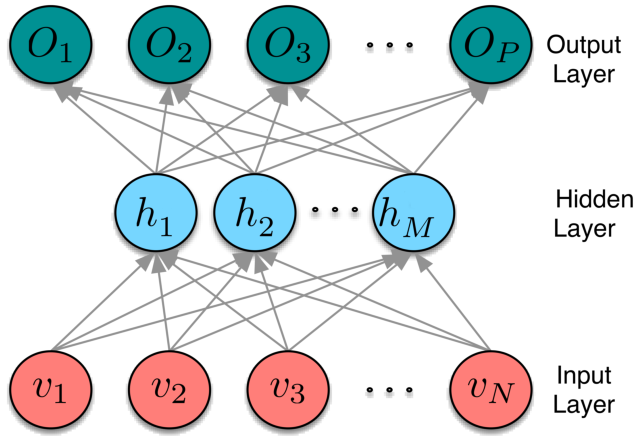
\includegraphics[width=.6\textwidth]{img/ML/MLP.pdf}
	\caption{General representation of a MLP}
	\label{fig:ML:MLP}
\end{figure} 

\section{Final considerations}
The design and development of the linking function need to take into considerations the domain and codomain of the addressed problems. The former needs to be shaped for the linking function, involving the regularization of the representation, and a possible expansion of the input space by means of kernel techniques. The linking function can be manually designed by means of rule-based techniques or learned by means of machine learning algorithms. We provided a background of rule-based techniques for the task of music structure analysis, which also involves the computation of the self-similarity and self-distance matrices as a useful representation of the music structure. We finally presented: a set of machine learning techniques for clustering, which involves unsupervised and semi-supervised techniques; distance learning techniques, in order to learn a semi-supervised distance metric for the input space; and completely supervised machine learning techniques to address codomain represented by discrete (classifiers) or continuous range (regressors).

%In the following chapters, we discuss a set of scenarios to model the music perception with increasing complexity. We employ the techniques described in Chapters \ref{Chap:LLFs}, \ref{Chap:HLFs} and \ref{Chap:ML}, to formalize the signal domain, the semantic codomain and to design a feasible and effective linking function.
\chapter{Formalization of the semantic domain}
\label{Chap:HLFs}
Music Information Retrieval aims at designing automatic systems to help users visualize, browse, analyze and retrieve songs in large music collections. In Chapter \ref{Chap:LLFs} we formalized the musical content, which is the signal domain of the problem, by means of a feature representation; in this Chapter we formalize the high-level meaning of music, which is the semantic domain, by analyzing the so-called \textit{High-Level Features} (HLFs). 

The user semantics of music is affected by personal taste and users' background, and therefore there is a certain degree of subjectivity. When developing models for the formalization of music semantics, we assume there exists an objective baseline, i.e., an interpretation of the high-level meaning that is shared by the majority of people. We make use of this assumption as a constraint for the analysis of the semantic domain. This constraint can be later removed by designing approaches that consider users' customization.

In Section \ref{sec:HLFs:categorical} we discuss the most intuitive way to formalize the semantic domain, i.e., the \textit{categorical} approach. This approach represents the HLFs as a set of classes and classifies a given song with the HLFs that are feasible to describe it. The semantics of the set of classes, and therefore of the HLFs, can be disjoint or overlapping.

The former scenario, discussed in Section \ref{sec:HLFs:class} involves to classify a song into non-overlapping categories that fully describe a semantic characteristic of music. As an example, a given song can either be classified as \textit{vocal} or \textit{instrumental}, or as a \textit{live performance} or \textit{studio recording}. This kind of classification is helpful to create a major distinction between songs. Due to the complex nature of music, however, it is rare to find a set of strictly non-overlapping categories. As an example, the categories induced by the genre taxonomy are not disjoint, due to the existence of \textit{cross-genre} songs.

It is possible to overcome this issue by using overlapping HLFs, as discussed in Section \ref{sec:HLFs:anns}, where each HLF describe a high-level aspect of music and a song is formalized as the set of HLFs that are commonly used to describe it. Back to the example about genre, we formalize the semantic domain as a set of genre-related HLFs, and a given song is represented by the set HLFs that are used to describe it, such as \textit{rock}, \textit{pop}, \textit{glam rock}, etc. 

The categorical approach has two main limitations. The first limitation concerns its use for the description of entire songs, that therefore does not take into consideration the time-variance of music semantics. The same HLFs might not be able to describe different sections of the song. As an example, the song \textit{Live and Let Die} by Paul McCartney contains a slow and melancholic \textit{intro}, and a groovy and reggae \textit{bridge}. The second limitation concerns the low level of expressiveness of the categorical approach. In natural language, indeed, it is common to express not only whether a HLF describes a certain song, but also its degree of descriptiveness. The graded description allows people to compare songs, e.g., to describe a song as \textit{faster} or \textit{less stuttering} than another. 

We address the former limitation by formalizing the semantic domain of the musical \textit{structure}. This formalization, indeed, allows us to refer to the \textit{sections} within the song that are likely to be semantically uniform, i.e., time-invariant with respect to the high-level description. In Section \ref{sec:HLFs:MSA} we discuss how the structure is formalized in the state of the art.

The second limitation is addressed by formalizing the semantic domain following a \textit{dimensional} approach. This approach identifies the degree of descriptiveness of each HLF for a given song. Such graded description effectively increases the expressiveness of the model, providing an explicit and easy way to perform the aforementioned comparison between songs.

From a dimensional formalization of the semantic domain, we define a \textit{semantic model} as the model that embeds the dimensional HLFs. 
In Section \ref{sec:HLFs:models} we briefly discuss some dimensional semantic models proposed in the MIR literature. In a traditional semantic model, the HLFs are defined as independent with each other. In natural language, however, the terms are often semantically related with each other. In order to consider such relation in the model, we can include a \textit{semantic space} where the similarity among HLFs is defined, by means of two main approaches: by manually defining the model, the terms and the similarity among terms; or by automatically inferring the space from annotated data. 

In Section \ref{sec:HLFs:VA} we discuss the Valence-Arousal (VA) model as a specific case of a manually defined semantic space. The VA model is the main model for emotional-related descriptors and the mostly used in the music emotion recognition subfield. We also introduce the main dataset of HLFs that is collected for the VA model.

With regard to the automatically inferred semantic space, the main approach is based on the Latent Semantic Analysis (LSA) applied on large collection of annotated data.
An important source of data are the \textit{social tags} that are annotated directly by the users in the Internet. We discuss LSA and its application in MIR in Section \ref{sec:HLFs:LSA}.

The two approaches are treated as mutually exclusive: either the semantic space is manually defined or it is automatically inferred. In this regard, in Section \ref{sec:HLFs:ANEW} we investigate a hybrid approach to improve a manually defined semantic space by including information that is inferred from annotated data. We focus on the Valence-Arousal model using LSA-based or manually collected information. This approach also contributes to enrich the defined space with some context specific to the music description scenario. This study was presented at the International Conference for Music Information Retrieval (ISMIR) \cite{Buccoli2016AHE},

For the sake of completeness, in Section \ref{sec:HLFs:ontology} we provide an overview of the most advanced formalization of the semantic domain, i.e., the ontologies, which aim at modeling the complete domain of knowledge of a given subfield.%, so  the state of the art is still in a beginning stage.

%The common approach to address music annotation is to define a set of HLFs for the semantic domain and use them to describe a music item with the set of meaningful HLFs.
%
%
%Consequently, the classification is frequently based on multiple, overlapping categories, that need to address several categories. 
%
%In order to do so, we define a set of HLFs, or \textit{tags}, that are used to model the semantic domain
%
%We can first refer to a semantic description that is close to the musical content, by considering the Music Structure Analysis (MSA), which concerns the identification of the segments within the song that can be grouped into categories named \textit{sections} based on their content. In Section \ref{sec:HLFs:MSA} we discuss how MSA provides a well defined and objective formalization for the semantic domain. 
%
%
%Two are the main approaches for the formalization of the semantic domain: the categorical approach and the dimensional approach. The former, described in Section \ref{sec:HLFs:categorical}, ; the latter, described in Section \ref{sec:HLFs:models}, identifies the degree of descriptiveness of a HLF for a music item.



%design a solving algorithm to automatically infer the classification for the descriptors within the set. 




%In the following we present the state of the art of the formalization of the semantic domain. We also provide a theoretical background on some tasks that are more relevant for this work. 




\section{Categorical description of music}\label{sec:HLFs:categorical}
\subsection{Disjoint classes}\label{sec:HLFs:class}
Due to the complexity and variety of the music semantics, the disjoint categorization of music is rather rare. Nevertheless, it has been addressed by the MIR community by constraining more general cases. An example is the case of classifying a song by performing artist. While different artists can perform the same song (the main and the \textit{featuring} artist), \cite{mandel2005song} presents an approach for artist identification obtained by composing a dataset of 1200 pop songs by a subset of 18 artists. In \cite{Bestagini2013b} the use-case of music classification between \textit{official live performances} and \textit{unofficial bootleg recordings} is discussed. The classification is made possible by composing the dataset with songs from only these two categories. In Chapter \ref{Chap:Bootleg} we analyze the complete scenario by adding the official studio recording category.

%cerca A Survey of Audio-Based Music Classification and Annotation

Some simple case of music emotion and genre recognition falls into the disjoint categorization. While the semantics of emotion is very rich and complex, and discussed in detail in Section \ref{sec:HLFs:VA}, some constraints can be added in this task. A common approach is to divide the emotion spectrum into a set of categories and then classify the emotional content of each song into one of these categories. In \cite{Hu:2007} the authors define five clusters for emotion-related descriptors: 
\begin{itemize}
\item \textbf{Cluster 1} Rowdy, Rousing, Confident, Boisterous, Passionate;
\item \textbf{Cluster 2} Amiable/Good natured, Sweet, Fun, Rollicking, Cheerful;
\item \textbf{Cluster 3} Literate, Wistful, Bittersweet, Autumnal, Brooding, Poignant;
\item \textbf{Cluster 4} Witty, Humorous, Whimsical, Wry, Campy, Quirky, Silly;
\item \textbf{Cluster 5} Volatile, Fiery, Visceral, Aggressive, Tense/Anxious, Intense.
\end{itemize}
%Cluster_1: passionate, rousing, confident,boisterous, rowdy
%Cluster_2: rollicking, cheerful, fun, sweet, amiable/good natured
%Cluster_3: literate, poignant, wistful, bittersweet, autumnal, brooding
%Cluster_4: humorous, silly, campy, quirky, whimsical, witty, wry
%Cluster_5: aggressive, fiery,tense/anxious, intense, volatile,visceral
These five clusters are used as a reference for several works on emotion classification \cite{Bischoff:2009, laurier2008multimodal, Laurier2009}.

The same approach is used for the formalization of semantics regarding the music genre: instead of addressing the complete and highly complex scenario of genre representation, some macro non-overlapping genres are defined and used as reference. In \cite{tzanetakis2002musical} the authors present a dataset for musical genre recognition base on a set of 10 genre descriptors: \textit{Blues}, \textit{Classical}, \textit{Country}, \textit{Disco}, \textit{Hip Hop}, \textit{Jazz}, \textit{Metal}, \textit{Popular}, \textit{Reggae}, and \textit{Rock}. This dataset has been used as a benchmark for genre recognition by a wide part of the community \cite{Sturm2012GTZAN}. In \cite{Scaringella2006} the defined genre are, instead, \textit{classical}, \textit{ambient}, \textit{electronic}, \textit{new-age}, \textit{rock}, \textit{punk}, \textit{jazz}, \textit{blues}, \textit{folk}, and \textit{ethnic}. This set of genres are effectively used as a broad categorization of musical content or as a constrained use-case to test real application scenarios. However, they are special or limited case that need to be eventually expanded.
%
\subsection{Overlapping categories}\label{sec:HLFs:anns}
In the categorical approach, the semantic domain is formalized as a set of multiple, independent HLFs, where each descriptor is only used or not used for the description of a song. It can be seen as a multi-label classification problem, where each classification concerns the presence or absence of a descriptor in a song. %More formally, instead of having one $N$-category classification, the music annotation concerns $N$ two-category classifications.

In \cite{wordsCAL500}, the authors define a set of 159 HLFs spanning several semantic aspects of music:
\begin{itemize}
\item \textit{emotion}: concerns feelings inspired by the songs; 
\item \textit{genre}: the musical genre of the songs;
\item \textit{instrument}: the instruments played during the song, including \textit{male} and \textit{female lead vocals};
\item \textit{song}: some high-level properties of the song, such as \textit{changing energy level}, \textit{catchy/memorable} ; 
\item \textit{usage}: typical situation for listening that particular song e.g., \textit{at a party}, \textit{going to sleep} and so on);  
\item \textit{vocals}: the style or features of the singer, such as \textit{duet} or \textit{breathy}.
\end{itemize}
This set of descriptors, together with the collected dataset described in \cite{Turnbull2007} (CAL500), have been widely used in the community for the task of music annotation \cite{coviello2011, nam2012learning,yeh2014improving}. The descriptors are treated as independent, while a strong correlation among them is highlighted by \cite{Miotto2012}, who suggest a generative model to exploit it.

A valuable source of information for music annotation is provided by the social tags. The \textit{tags} are free-text labels that are largely used in blogs, forum and social networks (as \textit{hashtags}) to classify content. They have been extremely used for music description as well, providing a tremendous amount of information for music researchers \cite{lamere2009}. In particular, the Internet web service Lastfm\footnote{www.lastfm.com} contributed to create and made available a large dataset of tagging information. Social tags can help to formalize the semantic domain with the categorical approach, with an amount of tags that is close to the number of words used in the natural language. The collection of tags from multiple users has been named \textit{folksonomy}, a taxonomy from the folk \cite{morrison2008tagging}. The social tags present several issues: the data is not structured and noisy, e.g., for different spelling (e.g., \textit{rock}, \textit{rock'n roll}, \textit{rock and roll}); the tags reflect the semantics of the users, so they include a certain degree of subjectivity;  each user follows their taste while tagging and it is hard to understand whether a certain tag describes the content of the music or a judgment by the tagger; malicious tags can be generated in the worst case scenario. Moreover, popular songs receive more annotations and tags, while less popular ones are likely not to be annotated \cite{lamere2009}. 
Nevertheless, the social tags have been extensively exploited by MIR researchers as a source of information and a definition of the semantic domain \cite{Celma2008,eck2008automatic,begelman2006automated,Levy2007}.

%The multi-label approach used in music annotation helps to formalize the semantic domain, since a. 
The  categorical approach is sufficient to formalize the semantic domain for several simple use-cases. However, this approach is not able to fully describe the semantics used for music, since it cannot model the intensity in the description. While the intensity might in fact be coded into the meaning of words, this strategy would implicitly rely on the objectivity of the words' semantics and on an extremely large set of descriptors. For this reason, in Section \ref{sec:HLFs:models} we discuss the dimensional approach, which leads to a simpler explicit modeling of the intensity.



\begin{figure}[tbp]
	\begin{center}
		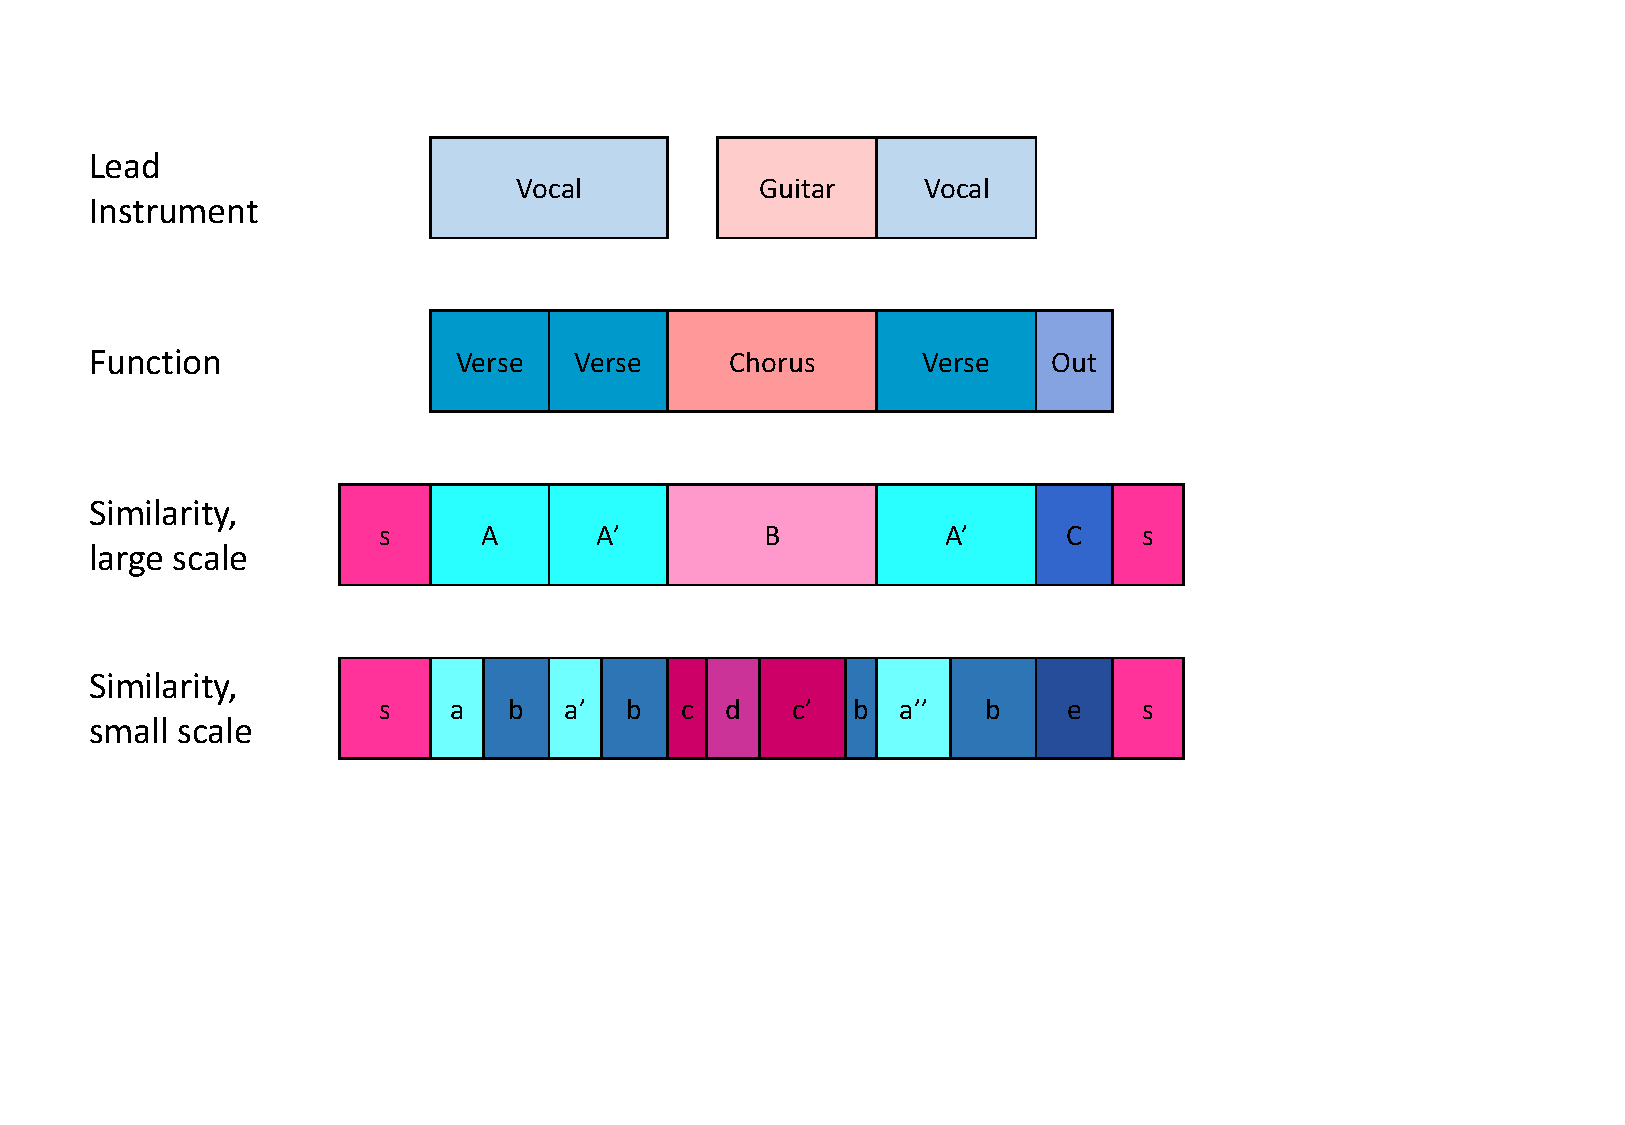
\includegraphics[trim=1cm 6cm 6cm 2cm,clip=true,width=\textwidth]{img/HLFs/functionColors}
		%\psfig{file=img/ML/logopm.jpg,width=3.5cm}
	\end{center}
	\caption{Example of the different labeling proposed in \cite{Smith2011}}
	\label{fig:HLFs:MSAscales}
	
\end{figure}

\section{Musical Structure Analysis}\label{sec:HLFs:MSA}
We infer useful information from the structure of a song, and the structure itself is in fact a high-level representation of it. In \cite{Smith2011} the authors present the dataset SALAMI, that is composed of structural annotations for around 1400 musical recordings. The authors also introduce several paradigms for the structural annotation (see Figure \ref{fig:HLFs:MSAscales}), that can be seen as structure-based HLFs:
\begin{enumerate}
	\item \textit{Lead Instrument} to identify the section based on the lead instrument (Vocal, Guitar, etc.);
	\item \textit{Function} to identify the section based on the semantic function, drawn from a set of 20 labels (see Table \ref{tab:HLFs:MSAfunctions});
	\item \textit{Similarity, large scale} does not add a semantics, it just uses letters to identify the sections. Similar sections, like two verses, are identified by the same letter;
	\item \textit{Similarity, small scale} focuses on shorter sections to identify them; the boundaries of the large scale match some of those in the small scale.
\end{enumerate}

The semantic domain for the problem of automatic MSA is particularly well formalized. However, automatic approaches perform only the boundary detection and grouping of similar sections, without annotating the song with the label \cite{ullrich2014boundary,Nieto2D,Nieto2016,NietoCNMF}, so the semantic domain in this case is not fully exploited. Moreover, the linking function from the signal domain is still not clear, as discussed in Section \ref{sec:ML:MSA}. We address the problem in Chapter \ref{Chap:MSA}.

\begin{table}[tbp]
\caption{List of labels for function-based MSA}
\label{tab:HLFs:MSAfunctions}
	\centering
	\large
	\bgroup
	\def\arraystretch{1.5}
	\begin{tabular}{||p{.25\textwidth}|p{.7\textwidth}||}
		\hline
		\hline
		\textbf{Group} & \textbf{Labels} \\
		\hline
		\hline
		Basic group & intro, verse, chorus, bridge\\
		\hline
		Instrumental & instrumental, solo\\
		\hline
		Transition & transition, pre-chorus, pre-verse, interlude\\
		\hline
		Genre-specific & head, main theme, (secondary) theme\\
		\hline
		Form-specific & exposition, development, recapitulation\\
		\hline
		Ending & outro, coda, fadeout\\
		\hline
		Special labels & silence, end\\
		\hline
		\hline
	\end{tabular}
\egroup

\end{table}

 \begin{figure}[tbp]
    \begin{center}
      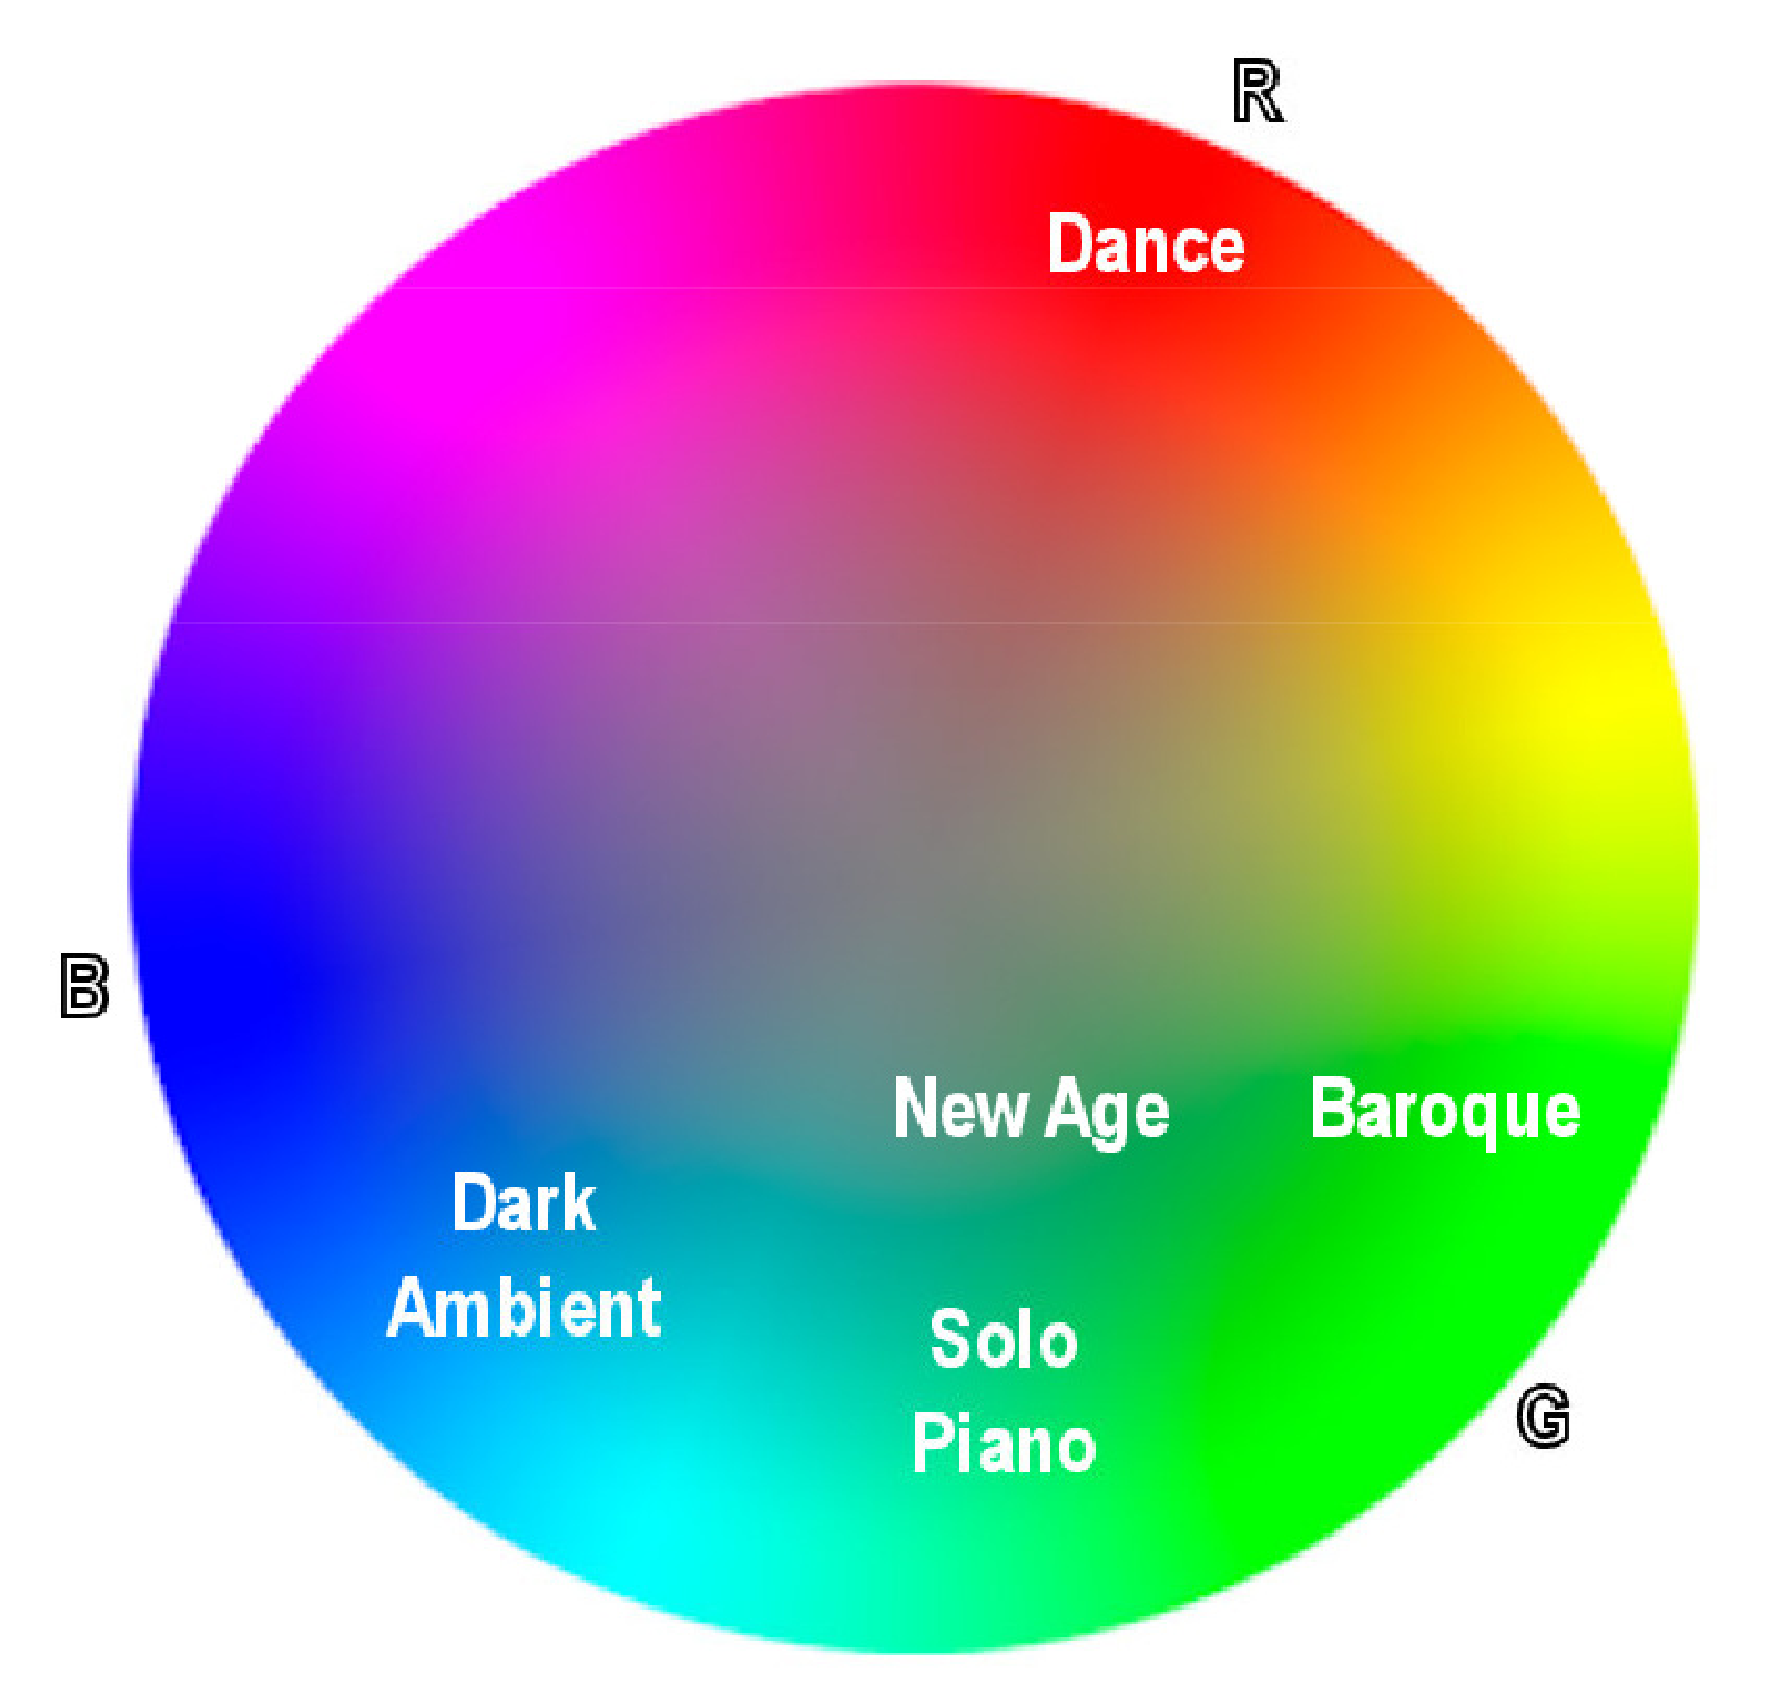
\includegraphics[width=8.5cm]{img/HLFs/triangleB}
	%\psfig{file=./pictures/logopm.jpg,width=3.5cm}
    \end{center}
  \caption{The 3D genre visualization from \cite{Prandi2009}}
  \label{fig:HLFs:prandi}
  \end{figure}


\section{Dimensional description of music and semantic models}\label{sec:HLFs:models} %dimensional}
%\subsection{Semantic Models}\label{sec:HLFs:models}
A dimensional semantic model concerns the use of a set of dimensional high-level descriptors, which allow to express the intensity of the description by using a continuous range of values. 

In \cite{Prandi2009} the authors identify three dimensional HLFs to represent music genres: \textit{darkness}, \textit{dynamicity} and \textit{classicity}. They use the three descriptors to span a 3D music genre space, where each genre is an area in the space, and areas can overlap. The three dimensions are also associated with the three basic color to design a visualization tool, as shown in Figure \ref{fig:HLFs:prandi}. 

In \cite{Buccoli2013} the authors propose a set of 9 bipolar dimensional HLFs to describe non emotional-related aspects of music: \textit{soft/hard}, \textit{clear/dull}, \textit{rough/harmonious}, \textit{void/compact}, \textit{flowing/stuttering}, \textit{dynamic/static}, \textit{groovy/not groovy}, \textit{easy/difficult} and \textit{fast/slow}. The non-emotional related content is represented in the model with a numerical value for each of the descriptor, and the HLFs are defined as independent with each other.

%The authors do not populate the model with terms, nor they define a semantic distance among descriptors, but the dimensionality of the model allows to define the intensity of the descriptors by using qualifiers from \cite{LIKERT} (e.g., \textit{moderately groovy}, \textit{extremely difficult}) and to define a semantic similarity metric between the representations of the songs.

A semantic model is refined by defining not only the set of descriptors, but also the semantic relations among them. Such semantic similarities are either manually designed or automatically inferred. With the former approach, a set of descriptors is chosen and some explicit or implicit semantic distance between them is defined. In Section \ref{sec:HLFs:VA} we discuss the most popular example of this approach, i.e., the Valence-Arousal semantic model for emotion representation. With the latter approach, some numerical or algebraic algorithms are applied on a set of data in order to infer a similarity metric. Several researchers have employed the Latent Semantic Analysis with this aim, so we discuss this approach in detail in Section \ref{sec:HLFs:LSA}.

 \begin{figure}[tbp]
    \begin{center}
      \includegraphics[width=8.5cm]{img/HLFs/VAmoods}
	%\psfig{file=./pictures/logopm.jpg,width=3.5cm}
    \end{center}
  \caption{The 2D Valence-Arousal emotion plane, with some emotional-related descriptors approximately mapped \cite{Yang2012}}
  \label{fig:HLFs:VAmoods}
\end{figure}

\subsection{The Valence-Arousal Model}\label{sec:HLFs:VA}
One of the fundamental properties of music is the ability to convey emotions\cite{Yang2012}. Consequently, the Music Information Retrieval community has been greatly interested in representing and classifying music according to emotions for music recommendation and personalization \cite{Barthet2012, Juslin:2001, Juslin2011, Lee2004, Yang2012}. Traditional meta-tags like artist or title are not informative on the content of a music piece and several studies \cite{Juslin:2001, Juslin2011, Lee2004, Yang2012} on user needs and behaviors have proven, in fact, the interest of representing and classifying music according to emotions. 

It has been proven, indeed, that listeners enjoy looking for and discovering music using emotion-based queries, which represents 33\% of music queries according to \cite{Lee2004}. This is an important reason that urged music psychologists and musicologists to investigate different paradigms for the representation and modeling of emotion related descriptors \cite{Juslin:2001, Juslin2011, Lee2004}. In \cite{Barthet2013} the authors review a high number of categorical and dimensional semantic models for music emotion recognition, including the one proposed in \cite{Russell1980}.

In \cite{Russell1980}, the authors propose a semantic model of emotions based on two dimensional descriptors, the Valence and the Arousal. The Valence indicates the graded polarization of the sentiment, from negative to positive, whereas Arousal estimates the degree of energy, or activation, in the emotion, from low to high. Emotional-related descriptors are modeled as a combination of Valence and Arousal and represented in the 2-dimensional VA space. The dimensional space allows a continuous shading of the formalization of the semantics of emotions, with some well defined areas such as represented in Figure \ref{fig:HLFs:VAmoods}: 
\begin{itemize}
\item joyful emotions are represented in an area with high arousal and positive valence; 
\item sad emotions are assigned with low arousal and negative valence;
\item aggressive emotions are represented in the high-energy, negative-valence portion;
\item calm emotions are defined as low arousal and positive valence sample.
\end{itemize}

The VA model can be used for mapping both HLFs and music (or any other) content. Since the VA model defines a dimensional space, a metric distance can be defined in order to model the semantic distance among descriptors, among the representation of the content, or even between descriptors and content. Given two generic items in the VA space $\mathbf{x}=[x_V,x_A]\T $ and $\mathbf{y}=[y_V, y_A]\T$, a simple distance metric is the Euclidean distance:
\begin{equation}
d(\mathbf{x},\mathbf{y})=\sqrt{(x_V-y_V)^2+(x_A-y_A)^2}.
\end{equation}

\begin{figure}[bt] 
	\centering 
	\includegraphics[width=0.75\columnwidth]{img/ANEW/ANEW.pdf}
	\caption{Distribution of the ANEW dataset in the VA space}
	\label{fig:HLFs:ANEW}
\end{figure}	

Some works propose a third dimension for the VA model \cite{Kim2010}, but no agreement has been reached within the community yet. While a third dimension potentially increases the precision of the model, it also increases its complexity and the cognitive load required for annotation. In \cite{bigand2005multidimensional} the authors propose a third dimension to represent the continuity or discontinuity of the emotion, or the melodic-harmonic contrast for music-related emotion description. In \cite{scherer2004emotions} the third dimension is identified as the \textit{dominance} (D), which expresses the degree of control of the emotion. Dominance allows to distinguish possibly overlapping emotions, such as fear and anger, that are both negative and active. While the VA space is more widely used \cite{Weninger2014, aljanaki2015emotion}, the Valence - Arousal - Dominance (VAD) space has received some attention as well \cite{Yang2012, Cowie2012, Scherer2004}. 

The increasing need of a continuous affective model led to the creation of the \textit{Affective Norm for English Words} (ANEW) dataset \cite{Bradley1999} for psychological research. This dataset is composed of 2,476 English words with positions in the VAD space. Albeit it is a generic dataset, the large amount of terms in ANEW makes it a powerful resource also for the Music Emotion Recognition (MER) community, including applications for automatic music annotation and retrieval \cite{Buccoli2013, Saari2015}. Unfortunately, ANEW terms in the VAD space tend to have a very uniform and compact distribution concentrated around the center of the space as shown in Figure \ref{fig:HLFs:ANEW} for the VA projection. 

Although the use of a substantial set of terms provides a very representative model of a large variety of emotions, to deal with a compact and cluttered distribution can be problematic in many musical applications. For this reason, typically only a subset of the terms is used, leading to a loss in the exhaustiveness of the model. In the following Section \ref{sec:HLFs:ANEW} we discuss the improvement of the ANEW dataset by adding annotations on the music semantics of the HLFs. Such annotations are, in fact, also automatically inferred by means of a Latent Semantic Analysis, which is described in the next Section.

\subsection{Latent Semantic Analysis}\label{sec:HLFs:LSA}
The semantic annotation scenario pictured in Section \ref{sec:HLFs:anns} defines the semantic domain, but it does not model the semantic relation among the descriptors. This issue is common in other information retrieval scenarios and has been addressed by generating a semantic space from annotated dataset, by means of Latent Semantic Analysis (LSA).

Given a dataset of items annotated with several HLFs, LSA builds a semantic model by inferring graded similarities among descriptors from the frequency with which they are used together in the annotation of items (\textit{co-occurrence}). As an example, if the descriptors \textit{quiet} and \textit{calm} are frequently used together and on the opposite, \textit{quiet} and \textit{aggressive} never co-occur, the LSA can infer that \textit{quiet} and \textit{calm} are highly similar, while \textit{quiet} and \textit{aggressive} are more likely to be opposite. More formally, the LSA is based on the approximation of the matrix that collects the annotations. Such an approximation is able to exploit the relations among the HLFs and among the tracks, leading to a novel vector space where each basis vector is a linear combinations of the original descriptors. The HLFs are therefore represented as a linear combination of the novel basis vectors, and the distance between such representations is related to the semantic relations of the underlying concepts \cite{Manning2008}. In Section \ref{app:LSA} we provide the technical background of the LSA.

In order to build a reliable semantic model, it is required to have access to a large annotated dataset. This is the reason why LSA has been effectively used with annotation from social tags, that collect annotations from thousands of users, for thousands of songs, with thousands of descriptors \cite{lamere2009}.

LSA-based approaches have been often employed by MIR community to derive semantic models from large annotated dataset. In \cite{Levy2007} the authors use tags collected from the last.fm and MyStrands web services to build a generic semantic space. In \cite{Celma2008} the author infers a dimensional space with LSA and exploits such novel space to define a metric of semantic similarity among annotated tracks. The works described in \cite{Laurier2009,saari2014semantic} focus on a semantic space for emotional-related descriptors and apply the LSA to obtain a lower-dimensional space for the HLFs. In particular, the authors of \cite{Laurier2009} compare the obtained space with the Valence-Arousal model, while the authors of \cite{saari2014semantic} apply multidimensional scaling to compute an automatic mapping from the LSA-based emotional-related HLFs to the Valence-Arousal space.

Although the LSA is a powerful resource to automatically define the semantic domain by means of a dimensional model, its use might rises some issues related to its use. First, the quality of annotations is crucial in this task, and social tags are often a noisy and unreliable source of information. Moreover, the LSA assumes that the co-occurrence of descriptors is related to their similarity, which is not always true. Finally, the phenomenon of \textit{polysemy}, i.e., a term with several meanings, is common in the natural language, and it is hard for LSA to infer the different meanings, which lead to different similarities among HLFs. In Chapter \ref{Chap:DCSM} we define a semantic model that can deal with different contexts, as sub-models, to address the issue of polysemy.

%

\section{An exploration of the semantic domain for emotional-related description}\label{sec:HLFs:ANEW}
In Section \ref{sec:HLFs:VA} we presented the Valence-Arousal (VA) model, which is one of the most widely used semantic model for the representation of emotional-related descriptors and content. The Valence is linked to the degree of pleasantness, while the Arousal represents the degree of excitement, or activation. A third dimension, related to \textit{Dominance} (D), is sometimes added to express the degree of control and to possibly distinguish different and overlapping emotions \cite{Cowie2012, Scherer2004}, leading to the Valence, Arousal, Dominance (VAD) space. In Section \ref{sec:HLFs:VA} we also discussed about the \textit{Affective Norm for English Words} (ANEW) dataset \cite{Bradley1999}, which is composed of almost 2,500 emotional-related descriptors mapped in the VAD space. While the dataset has been a helpful resource for the MIR community, it was not specifically designed for music description, and therefore its use presents some difficulty related to the distribution of terms and to the semantic relation among terms. As an example, it is not sure whether the metric of distance defined in the VA/VAD space can match the semantic similarity for the context of music description. Moreover, due to the clutter distribution of terms (see Figure \ref{fig:HLFs:ANEW}) it is difficult to conceptually organize them into a  hierarchy that is closer to how people describe music.

% \begin{figure}[bt] 
%   \centering 
%   \includegraphics[width=0.9\columnwidth]{img/ANEW/ANEW.pdf}
%   \caption{Distribution of the ANEW dataset in the VA space}
%   \label{fig:ANEW:ANEW}
% \end{figure}  


%In this scenario, the domain and the codomain of the problem both lie in the semantic world, and we aim at finding a linking function that is able to shape the VA or VAD semantic model to the novel space.

In this Section, we investigate the production of a novel emotional space, where the terms from ANEW dataset are better conceptually organized and bear more relevance for music description. Such emotional space would be highly helpful for the development of novel music application that rely on high-level emotional-related descriptors. In this study we build the new emotional space by taking advantage of kernel expansion techniques applied to the VA and VAD space, in order to design higher-dimensional emotional spaces.  Although the kernel transformation has the effect to produce a more sparse distribution of terms, it is not clear if the  semantic distance between concepts is well represented by the metric in the new space. We then use the prior information on music description to find a distance reflecting conceptual organization of terms by applying distance learning techniques \cite{xing2003distance, bar2003learning, goldberger2004neighbourhood}, as discussed in Section \ref{sec:ML:dist}. Given some constraints between terms, these methods search for a linear transformation of the space that is semantically relevant. That is, the ideal learned distance closely correlates with semantic differences given by users in a specific task for a subset of the ANEW terms. 

We generate the set of constraints using ``a priori'' information collected through a subjective test where participants were asked to specify the semantic similarity between pairs of terms in the context of music. We then perform Latent Semantic Analysis on emotion related annotations for a large set of music pieces. 

Under the hypothesis that the position of the terms in the space may be improved by this transformation, we validate the approach by grouping (i.e.,  clustering) the descriptors in the new high-dimensional space. In order to isolate the effect of distance learning from the use of apriori constraints, we use both unsupervised clustering techniques and semi-supervised clustering techniques. The latter make use of the same kind of constraints to retrieve the clusters with more relevance to the music semantics. We subsequently evaluate the resulting clusters with objective and subjective metrics. Tests show promising results given these new learned distance metrics and provide an insight into how a better configuration in the high-dimensional space can be achieved. 


 \begin{figure}[tb] 
  \centering 
  \includegraphics[width=0.95\columnwidth]{img/ANEW/scheme4.pdf}
  \caption{Block diagram of the clustering approach}
  \label{fig:ANEWblockdiag}
 \end{figure} 

Figure \ref{fig:ANEWblockdiag} shows the scheme of this work. We discuss the collection and generation of the annotated data and the building of the constraints to embed semantics about music in the learned distance metrics. We provide some quick details on the kernel expansion and distance learning techniques, since a more extensive description was presented in Sections \ref{sec:ML:kernels} and \ref{sec:ML:dist}, respectively. We then present the clustering techniques and the numerical results on the resulting clusters. Finally, we draw some overall considerations on the work.
%

In the following discussion, we will refer to \textit{emotion} and \textit{mood} as synonyms, as it is sometimes done in the natural language. It is worth remembering, however, that the two terms have different meanings. In \cite{Beedie2005} the authors investigate the difference between the meaning of the two terms by means of questionnaire proposed to non-academia participants and by reviewing the research works of the relating literature. The authors identify sixteen high-order themes of difference, such as \textit{duration} (moods have a generally considered to last longer),  \textit{awareness of cause} (the emotion is usually solicited by an identifiable source, while mood is often inexplicable), or \textit{display} (moods are considered rather personal, while emotions are more easy to be identified from an external observer). It is therefore hard to define a unique distinction between the meaning of the two terms. We will use \textit{mood} as a synonym of \textit{emotion} and, therefore, we will refer to the meaning of the latter for both terms.

\begin{table}[tb]
\caption{Summary of the collected data}
\label{tab:ANEWdata}
\begin{center}
\bgroup
\def\arraystretch{1.5}
\begin{tabular}{ ||p{.12\columnwidth} |l |p{.13\columnwidth}  |p{.50\columnwidth}||}
% \hline
\hline
\hline
Type &  Symbol & Num Terms & Details \\
\hline
\hline
Terms Dataset  &$\mathcal{D}_{\text{ANEW}} $ %=\{\mathbf{w}_1, ..., \mathbf{w}_N\}$
& 2,476 & Mean in V, A, D dimensions\\
% \hline
\hline
Implicit Distance  &$\mathbf{D}_{\text{ILM10K}}$& 240; 450 & Tag compact representation from an LSA with $k=10,20,50,100$ components\\
\hline
Explicit Distance  & $\mathbf{D}_{\text{HD}} $ & 180 & Human annotation of semantic similarity between terms from ANEW\\
\hline
Explicit Clustering  & $\mathbf{M}_{\text{HC}} $ & 100 & Human clustering of a subset of ANEW\\
\hline
\hline
% \hline
\end{tabular}\quad
\egroup
\end{center}
\end{table}


\subsection{Collection of the dataset}\label{sec:ANEW:data}
In this section, we describe three datasets created to provide the constraints for distance learning as well as to validate our approach. A summary of the collected data is provided in Table \ref{tab:ANEWdata}.

\subsubsection{Terms in the ANEW Dataset}
The terms in the ANEW dataset \cite{Bradley1999} are already annotated for the Valence, Arousal and Dominance dimensions with a value between 0 and 10 by psychology class students. We will refer to the ANEW dataset as
\begin{equation}
\mathcal{D}_{\text{ANEW}}=\{\mathbf{w}_1, ..., \mathbf{w}_T\}
\label{eq:ANEW:ANEW}
\end{equation} 
with $\mathbf{w}_i=\{\mu_V, \mu_A, \mu_D \}$, where $\mu_V$, $\mu_A$ and $\mu_D$ are the normalized average (between 0 and 1) of the annotations for the Valence, Arousal and Dominance descriptors respectively, and $T=2476$ is the number of terms in the ANEW dataset.  Specifically, we will refer to $\mathcal{D}_{\text{ANEW}}^{(VA)}$ and $\mathcal{D}_{\text{ANEW}}^{(VAD)}$ as the dataset with only Arousal and Valence dimensions considered and the dataset with also Dominance considered, respectively. 

\subsubsection{Implicit Distance Annotation}\label{sec:ANEW:ILM}
In Section \ref{sec:HLFs:LSA} we explained how we can perform  Latent Semantic Analysis (LSA) on an annotated dataset in order to infer a dimensional semantic space, which defines a metric of similarity among songs or terms. In this study, we compute a distance matrix among emotion related descriptors by performing LSA on a dataset composed of 10,199 tracks annotated with editorial and crowd sourced social tags, named I-Like-Music dataset, or ILM10K \cite{Saari2015, Allik2016}.
The dataset is annotated with weights corresponding to the prevalence of each tag in each song description. 

From the tags in ILM10K, we first discard the tags that are not included in the ANEW dataset. We then filter the tags that are rarely used by thresholding the frequency with which the tag  was used in ILM10K. We empirically choose the two thresholds as $15$ and $5$ times, leading to a set of $T=240$ and $T=450$ terms respectively. The former vocabulary contains less terms, but it is more reliable since they have been used quite often, while the latter is richer but the carried information might be less relevant. 

We build two tag-track matrices for the two sets $T=240$ and $T=450$, i.e., two matrices $\mathbf{A}_{\text{ILM10K}}^{(240)} \in \mathbb{R}^{240 \times 10199} $ and $\mathbf{A}_{\text{ILM10K}}^{(450)} \in \mathbb{R}^{450 \times 10199} $, respectively. We compute the $k$-component approximation of each matrix via LSA. We keep different numbers of components $k=10, 20, 50, 100$ to test different degrees of approximation, and we produce eight matrices $\mathbf{A}_{\text{ILM10K}}^{(T,k)} \in \mathbb{R}^{T \times k} $, one matrix for each combination of $T$ and $k$. 
 
Given a generic approximated matrix $\mathbf{A}_{\text{ILM10K}}$ (i.e., neglecting the notation about $T$ and $k$ for the sake of clarity), we compute two distance matrices between tags, using the Euclidean distance between the corresponding rows, producing the matrix  $\mathbf{D}_{\text{ILM10K}}$, and between the normalized rows (i.e.  $\mathbf{\tilde{A}}_{\text{ILM10K}}$), producing the matrix $ \tilde{\mathbf{D}}_{\text{ILM10K}}$. The latter matrix can be seen as a kind of transformation of the distance matrix using the Cosine-like distance. 

This procedure can also be interpreted as a Principle Component Analysis (PCA) \cite{Kim2005} and in fact PCA and LSA are two applications of the Singular Value Decomposition. From a (cleaned) tag-track matrix, we identify the $k$ principle linearly independent components from a linear combination of the $10,199$ tracks over the tag space. This procedure allows us to infer the similarity among tags from their use in the annotation task. 

\subsubsection{Human Distance Annotation}
\label{sec:ANEW:HDA}
We conducted an online survey to collect information on how people think of and rate the actual semantic similarity among emotional-related descriptors in the music context. We composed a subset of $T=240$ terms from the ANEW dataset as described in the previous Section \ref{sec:ANEW:ILM}. Each participant was asked to define the perceived emotional similarity in the context of music between pairs of descriptors with a value between $0$ (not similar at all) and $1$ (very similar). The pairs of descriptors proposed to the participants were randomly picked from the $T(T-1)/2$ possible combinations. We collected  
the received annotations and we inverted the score so that $0$ becomes the value for maximum semantic similarity and vice versa, in order to make the annotations consistent with the data described in Section \ref{sec:ANEW:ILM}. 

It is worth highlighting that the ANEW dataset collects annotation on the positions of emotional-related descriptors in the VAD space and the semantic similarity among terms is inferred by defining a metric of distance among the corresponding positions. The Human Distance Annotation aims to collect such semantic similarities by asking participants to explicitly annotate them.

504 people, either native or fluent English speakers, participated in the survey. Due to the high-number of possible pairs of terms, only a subset of them was annotated. In order to make the annotation more robust and reliable, we considered the pairs that received at least 2 annotations and the terms that belong to such pairs, leading to $T=180$. With the collected annotations, we compose the sparse matrix $ \mathbf{D}_{\text{HD}}$.

\subsubsection{Human Clustering Annotation}
\label{sec:ANEW:HCA}
Since we evaluate our approach by clustering the terms in the ANEW dataset in the original and new space, we also collected data on how people organize and group the emotional-related descriptors.

Therefore, we conducted a second online survey and asked annotators to group a subset of emotional-related descriptors. We selected a small subset of $T=100$ descriptors, in order to ease the cognitive load required for the manual grouping of the terms. The subset was composed of the most used tags in the ILM10K dataset. 

During the survey, we did not provide a fixed number of clusters, nor any suggestion or guideline, in order to collect the most possible unbiased annotations. At first, the participants were presented with the list of $100$ descriptors and an empty list of clusters. Testers were able to create as many clusters as they felt to need for their organization. 

$15$ people participated in the online survey, leading to the matrix $\mathbf{M}_{\text{HC}} $ with $T=100$ terms, where each entry $(i,j)$ indicates the number of people that grouped together the $i$-th and $j$-th terms. 

The number of participants that conducted the second survey is sensibly lower with respect to the first survey on the distance annotation. This is probably due to the high cognitive load of the task and the impossibility to use partially-annotated information. However, the information provided by $\mathbf{M}_{\text{HC}}$ is actually rich enough for the scope of our work. Indeed, while the matrix $ \mathbf{D}_{\text{HD}}$ is a sparse matrix, i.e., some pairs of terms might have not received any annotation, the matrix $\mathbf{M}_{\text{HC}} $ is a full matrix. Whenever $\mathbf{M}_{\text{HC}}(i,j)=0$, we can infer that all the $15$ participants have annotated that the $i$-th and $j$-th terms are too semantically dissimilar to be grouped in the same cluster. 

Please note that we refer to the annotations on clustering as $\mathbf{M}_{\text{HC}}$ since it indicates a similarity matrix, where the higher $\mathbf{M}_{\text{HC}}(i,j)$, the higher the similarity between the $i$-th and $j$-th terms, while we define $\mathbf{D}_{\text{HD}}$ and $\mathbf{D}_{\text{ILM10K}}$ as distance matrices.

\begin{figure}[bt] 
  \centering 
  \includegraphics[width=0.80\columnwidth]{img/ANEW/pearson_dist_3.pdf}
  \caption{Absolute Pearson Correlation between the values of the distance matrices computed or collected from different sources of data.}
  \label{fig:ANEWdistData}
\end{figure}  

\subsubsection{Preliminary considerations on data}
We perform a preliminary statistical analysis of the collected data. We compute two self-distance matrices from the datasets $\mathcal{D}_{\text{ANEW}}^{(VA)}$ and $\mathcal{D}_{\text{ANEW}}^{(VAD)}$ using the Euclidean distance. We also consider the matrices computed or collected in Section \ref{sec:ANEW:data}, considering, for the ILM10K dataset, only $T=240$, since they are the most robust annotations. Finally, for each combination of pairs of matrices, we compute the absolute Pearson correlation between the values of the two matrices. In the case of the matrix $\mathbf{D}_{\text{HD}}$, which is sparse, we only considered the actual data of the matrix in the computation of the Pearson correlation. In Figure \ref{fig:ANEWdistData} we show the absolute Pearson correlations between the self-distance matrices from different sources of data we collected. 

We can see that there is absolutely no correlation between the Euclidean distance defined in the VA or VAD space and the one that can be inferred from the LSA of the ILM10K dataset. Moreover, it exhibits a modest correlation also with the human distance annotation. This confirms the need of a new space for the ANEW dataset which is more relevant for the music description.

\subsection{Learning the high-dimensional semantic space}
\label{sec:ANEW:moodtag}
In \cite{Barthet2013DesignAE} the authors investigate the existent semantic mood models for music recommendation and assess that two or three dimensions are not sufficient to producing a discriminative space for large music libraries. For this reason, we aim at producing a new space for the ANEW dataset by exploiting high-dimensional transformations of the VA or VAD space. In order to do this, we employ kernel expansions and distance learning techniques, as presented in Sections \ref{sec:ML:kernels} and \ref{sec:ML:dist}.

With respect to the techniques of kernel expansion, we employ the polynomial (degree 2 and 3) and RBF kernels described in \ref{sec:ML:kernels} in their explicit form. We also consider two non high-dimensional cases:
\begin{itemize}
\item we use the simple data in $\mathcal{D}_{\text{ANEW}}$ as-is, in order to take into consideration the non-expanded case and compare the new space with the traditional VA or VAD space;
\item we make use of the $L^2$ normalized data, by composing the dataset $\tilde{\mathcal{D}}_{\text{ANEW}}$ with the terms $\{\tilde{\mathbf{w}}_1,..., \tilde{\mathbf{w}}_T \}$, where each term is the $L^2$-normalization of the terms in $\mathcal{D}_{\text{ANEW}}$, i.e., 
\begin{equation}
\begin{split}
\tilde{\mathcal{D}}_{\text{ANEW}} &=\{ \frac{\mathbf{w}_1}{||\mathbf{w}_1||},..., \frac{\mathbf{w}_T}{||\mathbf{w}_T||}  \}\\
&=\{\phi(\mathbf{w}_1), ..., \phi(\mathbf{w}_T)   \},
\end{split}
\end{equation}
with the terms defined in Equation \ref{eq:ANEW:ANEW}.
\end{itemize}

With regard to the distance learning techniques, we employ the discussed techniques \cite{Carey2015}, i.e., Iterative Projection\cite{xing2003distance} (IP); Relevant Components Analysis \cite{bar2003learning} (RCA); Neighborhood Components Analysis \cite{goldberger2004neighbourhood} (NCA). We use the distance learning techniques to learn the subspaces defined by $\mathbf{L}$, with $\mathbf{L}\T \mathbf{L}=\mathbf{A}$ the Mahalanobis matrix, in order to find the (possibly) high-dimensional emotional space as a mapping: $\mathbf{L} \cdot \phi ( \mathbf{w}_t) $ with $t=1,...,T$. As discussed in Section \ref{sec:ML:dist}, in order to train the distance learning techniques we require a set of constraints as two sets of samples Must-Link $ML$ and Cannot-Link $CL$; the former indicate which samples must be placed together and the latter indicate which samples should be placed far apart. In the following Section, we explain the procedure we used to create such constraints.

\subsubsection{Constraints Building}
\label{sec:ANEW:constraints}
We build different sets of constraints from each implicit or explicit annotations we presented in Section \ref{sec:ANEW:data}.

Firstly,  we compute the ML and CL constraints from the ILM10K dataset (Section \ref{sec:ANEW:ILM}) by thresholding the values in the (possibly normalized) distance matrices $\mathbf{D}_{\text{ILM10K}}^{(T,k)}$, for every $T=\{240; 450\}$ and $k=10,20,50,100$. We first compute the mean value $\mu_{\text{ILM10K}}^{(T,k)}$ and standard deviation $\sigma_{\text{ILM10K}}^{(T,k)}$ of the values.
Given the generic matrix $\mathbf{D}_{\text{ILM10K}}$ , we define the two thresholds as $th_l= \mu_{\text{ILM10K}} - 2 \sigma_{\text{ILM10K}} $, $th_h= \mu_{\text{ILM10K}} + 2 \sigma_{\text{ILM10K}} $ (we neglect the notation of the matrix on the threshold for the sake of clarity).  We compose the set of ML constraints by considering those pairs of terms which are close in the space defined by LSA, hence whose distance is lower than $th_l$, and the CL set with those pairs of terms that are far from each other, i.e., whose distance is higher than $th_h$, i.e.:
\begin{equation}
ML=\{ (i, j) : \mathbf{D}_{\text{ILM10K}}(i,j)<th_l    \};
\end{equation}
\begin{equation}
CL=\{ (i, j) : \mathbf{D}_{\text{ILM10K}}(i,j)>th_h    \}.
\end{equation}
We compose the same sets of constraints from the normalized matrices $\mathbf{\hat{D}}_{\text{ILM10K}}$.

We use a similar approach to compose the ML and CL constraints from the Human Distance annotations. We compute the mean value $\mu_{\text{HD}}$ and standard deviation $\sigma_{\text{HD}}$ of the annotations in the matrix $\mathbf{D}_{\text{HD}}$ and we empirically define the thresholds $th_l=\mu_{\text{HD}} - \sigma_{\text{HD}},\; th_h=\mu_{\text{HD}} + \sigma_{\text{HD}}$ . In this case, the value of $\sigma_{\text{HD}}$ is higher than the ones obtained from the ILM10K distance $\sigma_{\text{ILM10K}}$, and therefore we choose a softer threshold and we do not use $2 \sigma_{\text{HD}}$.

Finally, from the Human Clustering annotations we compute the mean value $\mu_{\text{HC}}$ and standard deviation $\sigma_{\text{HC}}$ of the non-zero entries of the matrix $\mathbf{M}_{\text{HC}}$, i.e., of the number of people who annotated two terms as belonging to the same clusters, and define the soft threshold $th= \mu_{\text{HC}} - \sigma_{\text{HC}} $. We compose ML with the pair of terms that have been grouped together by more than $th$ people and we compose CL with the zero entries of $\mathbf{M}_{\text{HC}}$.

\subsection{Experimental setup}
\label{sec:ANEW:results}
As previously discussed, our aim is to find a transformation of the ANEW space with improved conceptual organization of terms that is relevant in a musical context. We expect terms that are semantically similar in this context to be close and dissimilar terms to be far apart. For this reason, we validate our approach by clustering the ANEW dataset in the transformed spaces. We employ some of the techniques described in Section \ref{sec:ML:clust}, specifically:
\begin{itemize}
\item the K-means algorithm  \cite{macqueen1967some};
\item the Spectral Clustering (SC) algorithm \cite{shi2000normalized};
\item the Agglomerative Hierarchical Clustering (AHC) algorithm \cite{sibson1973slink};
\item the Semi-Supervised Non-Negative Matrix Factorization (SS-NMF) algorithm \cite{chen2008} .
\end{itemize}

%A clustering algorithm is a machine learning technique that aims at grouping together the samples that are close together in a given space, where their distance is defined by some metric. In order to provide a robust evaluation, we apply several clustering techniques: the K-Means, the Semi-Supervised Non-Negative Matrix Factorization, the Spectral Clustering and the Agglomerative Hierarchical Clustering.

%The K-Means \cite{macqueen1967some} is a common unsupervised clustering algorithm, which first defines a centroid for each cluster and then assigns the samples to the closest centroids, i.e., to the correspondent cluster. The position of the centroids are adjusted to be the actual centroid of the assigned samples and the assignment is ran again. This two steps procedure is ran for several iterations until convergence. While K-Means algorithm is effective to retrieve clusters with a globular shape \cite{PAMI} (i.e., with similar variance in all the dimensions), the distance learning techniques can provide a better separation of clusters and address the issue.

%The Semi-Supervised Non-Negative Matrix Factorization \cite{chen2008} (SS-NMF) applies the Non-Negative Matrix Factorization discussed in Section \ref{sec:ML:MSA} for the case of Music Structure Analysis. The NMF is able to decompose a matrix into a sum of components; in this case, the self-distance matrix of the terms in the new space is factorized in order to retrieve the main components, i.e., the main clusters. 

%The Spectral Clustering \cite{shi2000normalized} (SC) technique was also presented in Section \ref{sec:ML:MSA}. As mentioned, a graph is built from the distance matrix, with the nodes given by the samples and the edges defined by the (possibly learned) distances between them. The SC technique looks for the lowest cost partition of the graph, by employing a low-dimension reduction of the distance matrix and applying the K-Means algorithm on it.

%Finally, Agglomerative Hierarchical Clustering \cite{sibson1973slink} (AHC) follows a bottom-up approach to build the clusters. At the first iteration, each sample is a separate cluster. Then, the two closest clusters merge together as a cluster with two samples. The clusters keep merging until the desired number of clusters is reached. 

%Clustering the samples is commonly a unsupervised task. However, some algorithms can be adapted to be trained in a semi-supervised fashion, as described in Section \ref{sec:ML:clust}. 
We use the SS-NMF, SC and AHC techniques with both the unsupervised and semi-supervised  approach, while using K-means with the purely unsupervised fashion, as explained in Section \ref{sec:ML:clust}.

%are able to include some apriori information by processing the distance matrix with some constraints. Given the generic distance matrix $\mathbf{M}$ and two sets of constraints $CL$ and $ML$ as defined above, we can include the constraints by computing the matrix $\mathbf{D}$ as:
%\begin{equation}
%\mathbf{D}=[\mathbf{M}(i,j)- \zeta_{i,j} + \vartheta_{i,j}] 
%\end{equation}
%where $\zeta_{i,j}\geq 0$ if $(i,j)$ is in the $ML$ set and $\vartheta_{i,j}\geq 0$ if $(i,j)$ is in the $CL$ set. This makes the samples in the $ML$ set closer and the samples in the $CL$ set further apart. In this work we empirically choose a constant value for all the distances, equal to half the range of the values in the matrix $\mathbf{M}$.

%In this study we use the SS-NMF, SC and AHC algorithms in both unsupervised and semi-supervised fashion. 

In order to validate the actual contribution of the distance learning techniques, we compare the results of our approach with the results obtained with both unsupervised and semi-supervised clustering of the ANEW dataset. Hence, we have three scenarios: 
\begin{enumerate}
\item the unsupervised clustering of the transformed (but not learned) space (\textbf{Unsup.});
\item the semi-supervised clustering of the transformed (but not learned) space (\textbf{SemiSup.}); 
\item our approach, that is the unsupervised clustering of the learned space (\textbf{Dist. Learn}).
\end{enumerate} 
It is worth remembering that the first scenario also includes the clustering of non-transformed space using the Euclidean distance. 

We perform the clustering over all the combinations of input, kernel expansion, constraints, distance learning and clustering techniques. Given the large number of configurations we need to test, we experimentally choose to retrieve the $6$ best representative clusters. In the following Section, we present the evaluation of the obtained clusters.

\subsection{Numerical results}
Since we have several configurations to test, and we do not have a full ground truth on the problem of clustering, we validate our approach by performing three different evaluations:
\begin{enumerate}
\item we use the objective metric called Silhouette index (Section \ref{sec:ANEW:obj_results}, Fig. \ref{fig:ANEWsilhouette}, Table \ref{tab:ANEWsilhouette}),  which perform a qualitative evaluation of the relation between the input data and the resulting clusters;
\item we compare the obtained clusters with the clustering of the samples defined by the rows of $\mathbf{D}_{\text{ILM10K}}$, in order to validate the degree of similarity between the clustering in the new space and the clustering in a space defined by music annotations (Section \ref{sec:ANEW:subILM10K_results}, Fig. \ref{fig:ANEWILM10K}, Table \ref{tab:ANEWv_score});
\item we compare the obtained clusters with the human annotation of clustering described in Section \ref{sec:ANEW:HCA} (Section \ref{sec:ANEW:subHC_results}, Fig. \ref{fig:ANEWF_measure}, Table \ref{tab:ANEWf_measure}).
\end{enumerate}

In the following, we separately discuss the three kinds of evaluation.

\begin{table}[tb]
	\caption{Best results for the Silhouette Index for each scenario}
	\label{tab:ANEWsilhouette}
%    \small
\begin{center}
  \bgroup
  \def\arraystretch{1.5}
\begin{tabular}{ ||l |l |l |l  |c||}
\hline
\hline
% \hline
Scenario & Features & Algorithm & Constraints & Silhouette \\
\hline
\hline
Unsup. & Norm. VA & kmeans & & 0.5287 \\
\hline
Semi-Sup. & Norm. VA & SC & $\mathbf{{M}}_{\text{HC}}$ & {\color[HTML]{8E0000} \textit{0.5240}} \\
\hline
IP Dist. & VAD & kmeans & $\mathbf{{D}}_{\text{HD}}$  & 0.5432 \\
\hline
RCA Dist. & VAD, poly 3 degree & AHC & $\mathbf{{M}}_{\text{HC}}$ & {\color[HTML]{326B00}  \textbf{0.6864}} \\
\hline
NCA Dist. & VA, poly 2 degree & kmeans & $\mathbf{\hat{D}}_{\text{ILM10K}}$, $T=240$, $k=10$ & 0.5456 \\
\hline
\hline
\end{tabular}\quad
\egroup
\end{center}
\end{table}



\begin{figure}[tbph]
  \centering 
  \includegraphics[width=0.85\columnwidth]{img/ANEW/Silhouette2.pdf}
  \caption{Boxplot of the Silhouette indices for the different scenarios}
  \label{fig:ANEWsilhouette}
\end{figure}  


\subsubsection{Objective metrics} \label{sec:ANEW:obj_results}
The Silhouette index is an objective quality metric that defines how much the clusters are compact and well separated. In order to do so, it defines for each sample $s$ a variable $a$ as the mean distance to all the samples in the same cluster and a variable $b$ as the mean distance to all the samples in the next nearest cluster. In order for a clustering to be well separated, $a$ should be small and $b$ should be high. The Silhouette index is hence computed as \cite{scikit-learn}:
\begin{equation}
\text{Silhouette}=\frac{1}{|\mathcal{D}|} \sum_{s \in \mathcal{D}} \frac{b-a}{\text{max}(a,b)}\in [-1,1],
\end{equation}
where $\mathcal{D}$ is the generic dataset of samples.  High (positive) values of Silhouette indicate dense well-separated clusters, values around $0$ indicate overlapping clusters and low (or negative) values indicate incorrect clusters. 

In Figure \ref{fig:ANEWsilhouette} we show the boxplots of Silhouette metric for the different scenarios, while in Table \ref{tab:ANEWsilhouette} we show the configurations that generate the best results for each scenario. 

It is clear that the application of Distance Learning techniques outperforms unsupervised and semi-supervised techniques, even with different configurations of kernels, algorithms and constraints. In particular, the best performance is obtained with the Agglomerative Hierarchical Clustering over the third degree polynomial expansion of the VAD dataset, with a translation learned using the RCA technique constrained by the data collected from the Human Clustering. 

From the boxplot we can see that the RCA distance learning presents some extremely high values of Silhouette, which are considered outliers. Nevertheless, even without the supposed-outlier configurations, the RCA technique achieves the highest results for the Silhouette index, while the NCA technique achieves the highest average result over the different configurations. 

We can also notice that the semi-supervised scenario performs on average worse than the unsupervised scenario. This is because the Silhouette index evaluates the resulting clusters with respect of the position of the input data, that is not moved from the original position. The estimated clusters are therefore more noisy, which confirms the advantage of distance learning techniques to transform the space.


\begin{figure}[tbp]
  \centering %\includegraphics[width=0.75\columnwidth]{img/ANEW/ILMVscore.pdf}
 \includegraphics[width=.85\columnwidth]{img/ANEW/ILMVscore_square.pdf}
  \caption{Completeness and Homogeneity results for the comparison of clusters with those obtained from the ILM10K dataset. Gray contour lines indicate the V-score}
  \label{fig:ANEWILM10K}
\end{figure}


\subsubsection{Subjective metrics - Comparison with Clustering of ILM10K}
\label{sec:ANEW:subILM10K_results}
Our proposed approach aims to draw from the ANEW dataset a new high-dimensional space that bears more relevance for the music annotation. In this regard, we compare the clusters obtained with the different approaches with clusters obtained directly from a music annotation scenario. In order to do so, we rely on the data inferred from the ILM10K dataset and apply the aforementioned unsupervised clustering techniques to the samples of $\mathbf{A}_{\text{ILM10K}}^{(T,k)}$ and $\mathbf{\tilde{A}}_{\text{ILM10K}}^{(T,k)}$ for the different $T$ and $k$. In this case, we have a set of predicted clusters and a set of ground truth clusters, and we want to estimate how much the former resembles the latter.  

We consider the homogeneity and completeness metrics \cite{rosenberg2007v}. The two metrics range between 0 and 1, and higher values correspond to better performance. More specifically, the homogeneity metric evaluates whether each estimated cluster contains only members of a group in the ground truth, while the completeness metric, instead, estimates whether the samples of a given group belongs to the same estimated cluster. The homogeneity and the completeness metrics are computed from the conditional entropy of the classes given the cluster assignment $H(C|K)$ and from the conditional entropy of clusters given class $H(K|C)$, respectively:
$$
	\text{homogeneity}=1-\frac{H(C|K)}{H(C)},
$$
$$
\text{completeness}=1-\frac{H(K|C)}{H(C)},
$$
with 
$$
H(C|K)=-\sum_{c=1}^{|C|}\sum_{[k=1]}^{|K|} \frac{n_{c,k}}{n} \log (\frac{n_{c,k}}{n_k}),
$$
$$
H(K|C)=-\sum_{c=1}^{|C|}\sum_{[k=1]}^{|K|} \frac{n_{c,k}}{n} \log (\frac{n_{c,k}}{n_c})
$$
the aforementioned conditional entropies and
$$
H(C)=-\sum_{c=1}^{|C|} \frac{n_c}{n} \log(\frac{n_c}{n}),
$$
$$
H(K)=-\sum_{k=1}^{|K|} \frac{n_k}{n} \log(\frac{n_k}{n}),
$$
the entropy of clusters from ground truth or estimation respectively, with $|K|$ the number of estimated clusters, $|C|$ the number of ground-truth groups, $n_c$ and $n_k$ the number of samples that belong or are assigned to the cluster $c$ or $k$, respectively, and $n_{c,k}$ the number of samples belonging to the $c$-th cluster and assigned to the $k$-th's one.
We also consider the V-measure, i.e., the harmonic mean of homogeneity and completeness. 

To avoid overfitting issues, we do not consider those configurations that are trained with the constraints generated from the ILM10K dataset. More specifically, we evaluate only the configurations generated from the expanded VA and VAD dataset using either distance learning techniques or semi-supervised clustering techniques with constraints generated from the Human Distance or Human Clustering annotations.


We show the distribution of results for the different scenarios in Figure \ref{fig:ANEWILM10K}, where each point is a different configuration. We can visually estimate there are some stripes in the distribution of results, which are probably caused by the different sets of ground truth generated by the different clustering techniques and datasets from the ILM10K dataset. 
We notice the results are fairly low, showing that the organization given by the expanded and possibly learned ANEW dataset is very different from that inferred from social tags on a real music annotation scenario. This confirms the low correlation shown in Figure \ref{fig:ANEWdistData} and the necessity to find a space for the ANEW dataset which is more useful for MIR applications. However, it is clear that our approach can only slightly improve the task. 


\begin{table}[tbp]
	\caption{Best results of the Homogeneity, Separation and V-measure metrics for the comparison with the clusters generated by the AHC from the normalized ILM10K dataset ($T=240$, $k=100$)}
	\label{tab:ANEWv_score}
    \small
\begin{center}
  \bgroup
  \def\arraystretch{1.5}
\begin{tabular}{ ||l  |l| l |l  |c|c|c ||}
\hline
\hline
Scenario    & Features    &  Alg.   & Constr.   & Compl.  & Hom.  & V-score \\
\hline
\hline
Unsup.  & VA, poly 3 degree & SC &  &  0.0877 & 0.1334 & 0.1058 \\
\hline
Semi-Sup. & VAD poly 2 degree & AHC     & $\mathbf{{D}}_{\text{HD}}$   & 0.0955 & 0.1347 & 0.1118 \\
\hline
IP Dist. & VA       & SC    & $\mathbf{{D}}_{\text{HD}}$     & 0.0929 & 0.1371 & 0.1107 \\
\hline
RCA Dist. & VAD & kmeans & $\mathbf{{D}}_{\text{HD}}$ & 0.0869 & 0.1290 & {\color[HTML]{8E0000} \textit{0.1038}} \\
\hline
NCA Dist.& VA, poly 2 degree & AHC & $\mathbf{{D}}_{\text{HD}}$   & 0.0959 & 0.1421 & {\color[HTML]{326B00} \textbf{0.1145}}  \\
\hline
\hline
\end{tabular}
\egroup
\end{center}
\end{table}

In Table \ref{tab:ANEWv_score} we list the configurations that lead to the best performance. Such configuration are able to achieve a V-Score between $0.1058$ and $0.1145$, which is quite low. From the range of the best results in the Completeness and Homogeneity values, we can infer that the best results are all generated from the same configuration of the ILM10K ground truth, i.e., the one composed by the Agglomerative Hierarchical Clustering on the normalized dataset with 240 terms and $k=100$. This configuration is the most informative and reliable one, since it has few widely-used tags and the highest number of components, i.e., the richest approximation of the original matrix.  

Moreover, we can also see that all the highest results have been achieved by using the constraints from Human Distance. We believe that the reason of this is the medium-high correlation between the Human Distance annotation and the normalized ILM10K dataset, as shown in Figure \ref{fig:ANEWdistData}.

The best results is reached using NCA technique with a AHC over the polynomial-expanded VA dataset. We can see that the dataset and the kernel is the same that obtained the second highest result for the Silhouette metrics in Table \ref{tab:ANEWsilhouette} for the NCA technique. Moreover, the AHC is also used for the two highest results in this case, the NCA distance learning technique and the Semi-Supervised clustering.

However, since all the results are rather low, we cannot draw meaningful conclusions from this evaluation.

\subsubsection{Subjective metrics - Comparison with Human Annotations}
\label{sec:ANEW:subHC_results}
We finally compare the obtained clusters with those collected from human clustering annotations (HC). For this case, we will use traditional Precision, Recall and F-Measure metrics, which focus more on the the correctly grouped terms rather than the correctly non-grouped ones, since the former are more specific and relevant.

We define the matrix $\mathbf{Y}\in \mathbb{R}^{T \times T}$ of HC annotation as $\mathbf{Y}(i,j)=1$ if the $i$-th and $j$-th samples are in the same cluster by thresholding the matrix $\mathbf{M}_{\text{HC}}$ with $th=\mu-\sigma$, similarly as in Section \ref{sec:ANEW:constraints}. We then compose the matrix $\hat{\mathbf{Y}}$ from the estimated clustering results, and we define the sets $TP$, $FP$ and $FN$ as:
\begin{equation}
TP=\{(i,j) : \mathbf{Y}(i,j)=\hat{\mathbf{Y}}(i,j)=1 \};
\end{equation}
\begin{equation}
FP=\{(i,j) : \mathbf{Y}(i,j)\neq 1=\hat{\mathbf{Y}}(i,j) \};
\end{equation}
\begin{equation}
FN=\{(i,j) : \mathbf{Y}(i,j)=1 \neq \hat{\mathbf{Y}}(i,j) \}; 
\end{equation}
with $i,j=1,...,T$ and  $i<j$ to avoid duplicate pairs of samples such as $(i,j)$ and $(j,i)$. The Precision, Recall and F-Measure as \cite{Manning2008}: 
\begin{equation}\label{eq:HLFs:P}
P=\frac{|TP|}{|TP|+|FP|}\in [0,1];
\end{equation}
\begin{equation}\label{eq:HLFs:R}
R=\frac{|TP|}{|TP|+|FN|}\in [0,1];
\end{equation}
\begin{equation}\label{eq:HLFs:F}
F=\frac{2 P R}{P+R}\in [0,1].
\end{equation}
The Precision indicates the ratio of correctly clustered samples with respect to all the clustered samples; the Retrieval indicates the ratio of correctly clustered samples with respect to the samples that were supposed to be clustered together; the F-Measure is the harmonic mean between the two measures that provides a useful compact metric. The balanced F-measure, indeed, achieves high values only when both Precision and Recall are assigned with high values, while if either $P=0$ or $R=0$, we obtain $F=0$ regardless to the other metric.  

To avoid overfitting, we evaluate only configurations that are not trained with the constraints generated from the human annotations on clustering.

\begin{figure}[tbp]
  \centering 
     \includegraphics[width=.85\columnwidth]{img/ANEW/F_measure_square.pdf}
  %  \includegraphics[width=0.7\columnwidth,height=5cm]{img/ANEW/F_measure.pdf}    
  \caption{Precision and Recall results for the comparison of clusters with those obtained from human annotation. Gray contour lines indicate the F-measure.}
  \label{fig:ANEWF_measure}
\end{figure}  

In Figure \ref{fig:ANEWF_measure} we show the distribution of results for the different scenarios and configurations. In general, Precision is higher than Recall, showing that the estimated clustering is not capable of retrieving all the correct groups, while it is effective of correctly estimating the clusters. The F-measures are mostly distributed between 0.3 and 0.5, which is an average result. In particular, we can notice two notable trends, one around $P=0.6$ and one around $P=0.8$.
However, we can clearly see that some configuration from RCA Distance Learning are able to improve the average Recall and achieve highest values of F-measure.  The F-measure is achieved by losing some effectiveness in the Precision, leading to a rather balanced performance between $P$ and $R$. We can see that at least $9$ RCA configurations obtained higher results than any other configurations, and only one Semi-Supervised technique achieves $F>0.5$. This consideration clearly shows that the distance learning techniques are more effective to embed the information from constraints to better organize the terms with respect to the music context. 

\begin{table}[tb]
	
	\caption{Best results for the Precision, Recall and F-measure metric for the comparison with the human annotated clusters }
	\label{tab:ANEWf_measure}
\begin{center}
  \bgroup
  \def\arraystretch{1.5}
\begin{tabular}{ ||l |l| l |p{.15\textwidth} |c  |c|c||}
\hline
\hline
Scenario    & Features    &  Algorithm  & Constraints     & P   & R   & F \\
\hline
\hline
Unsup.  & VAD, RBF & kmeans     &          &  0.8012 & 0.3512 & {\color[HTML]{8E0000} \textit{0.4883}} \\
\hline
Semi-Sup. & VAD, RBF & AHC    & $\mathbf{{D}}_{\text{HD}}$     & 0.7646 & 0.3986 & 0.5240 \\
\hline
IP Dist. & VAD, RBF & AHC     & $\mathbf{\hat{D}}_{\text{ILM10K}}$, $T=240$,$\quad \;$ $k=100$ & 0.6979 & 0.3915 & 05016 \\
\hline
RCA Dist. & VA, poly 3 degree & AHC & $\mathbf{\hat{D}}_{\text{ILM10K}}$, $T=240$,$\quad \;$ $k=50$ & 0.6622 & 0.7241 & {\color[HTML]{326B00}  \textbf{0.6918}} \\
\hline
NCA Dist.& VAD, RBF & kmeans & $\mathbf{\hat{D}}_{\text{ILM10K}}$, $T=240$,$\quad \;$ $k=10$ & 0.7971 & 0.4124 & 0.5289  \\
\hline
\hline
\end{tabular}\quad
\egroup
\end{center}
\end{table}

In Table \ref{tab:ANEWf_measure} we list the best configurations for each scenarios. The RCA Distance Learning technique clearly outperforms the other approaches and matches very closely the human annotations, i.e., the way people organize the emotional-related descriptors. We can notice that once again, the best results are obtained by using the AHC over some polynomial expansion of the dataset. Moreover, all the distance learning techniques take advantage of the constraints generated from the most informative set of annotations, i.e., the normalized ILM10K dataset with fewer terms. In this scenario, however, lower components are required to achieve higher results: the RCA distance learning achieves its best results with $k=50$ components and the NCA distance learning with just $k=10$ components.

\subsection{Final remarks}\label{sec:ANEW:conclusions}

In this Section we investigated a possible formalization of the semantic domain as a dimensional semantic model for emotional-related descriptors. While the VA model and the ANEW space have been used in the MIR community for several years, this study proposed an useful approach to improve its ability of describing and possibly retrieving musical content by including information inferred from annotated dataset.

We introduced a novel approach consisting of kernel expansion, constraint building from task specific human annotation and finally distance learning to transform the ANEW dataset and obtain a distribution of terms that provides better conceptual organization with respect to the conventional VA or VAD spaces.

We validated our approach by evaluating its ability to conceptually organize the terms by performing some clustering techniques on the expanded and learned space, using subjective and objective evaluation metrics. We evaluated our proposed approach in a high-number of configurations, which we grouped into three main approaches: unsupervised clustering of the expanded space, semi-supervised clustering of the expanded space and unsupervised clustering of the learned expanded space. For each approach and for each metric we showed 
the average and the maximum results over the configurations. The average and maximum results prove that the use of distance learning techniques improves the position and therefore the organization of concepts of the ANEW dataset. In particular, agglomerative hierarchical clustering of a RCA-learned space based on the polynomial expansion of VA/VAD space outperforms the other configurations. 




\begin{figure}[bt] 
	\centering 
	\includegraphics[width=\textwidth]{img/HLFs/ontology.pdf}
	\caption{An example of a definition in an ontology \cite{Raimond2007}}
	\label{fig:HLFs:ontology}
\end{figure}	

\section{Ontologies}\label{sec:HLFs:ontology}
In the formalization of the semantic domain, a semantic model can effectively tackle the complexity of the natural language, by defining the set of descriptors and their semantic relations. In principle, we would like to be able to model all the kind of relations among descriptors, such as the notion of "composition", or how the music genre is related to some emotion-based features. In order to formalize the semantic domain, we need in fact to model the full knowledge of music. 

In computer and information science, an \textit{ontology} is a structural framework that models the representation of knowledge as a set of concepts \cite{Bechhofer2009}. An ontology can model a richer information with respect to semantic models, because it allows to hierarchically organize the semantic domain. A subset of the knowledge defined by an ontology, can be modeled and defined as an ontology itself.

The ontologies are a promising step toward a full definition of the semantic domain, although they require a considerable effort and the literature has not yet defined a set of reliable automatic tools to define or populate it. In \cite{Raimond2007} the authors present an ontology for editorial, cultural and acoustic music information. In Figure \ref{fig:HLFs:ontology} we show the description of a music production work flow from \cite{Raimond2007}, which explicits the complexity of modeling an ontology. In \cite{Zanoni2014} the authors present an ontology for the formalization of the knowledge on violin instruments as a part of a wider ontology on bowed instruments, which we use to formalize a semantic model in Chapter \ref{Chap:Violin}. In \cite{ElRaheb2012} the authors introduce an ontology for representing dance movements.  

\section{Final considerations}
We provided an overview of  different approaches used in the MIR literature to formalize the semantic domain of the musical content, by means of high-level features. These approaches have different levels of complexity, depending on the problem addressed. We discussed the two main approaches for the more abstract and subjective description, i.e., the categorical and the dimensional approaches. We presented the categorical approach, that defines the semantic domain as a set of disjoint or overlapping categories. The categorical approach has however some limitations in its descriptive power, due to the graded descriptions of natural language. Moreover, due to the time variance of music, the description of entire songs is also limited. We provide an overview of the semantics of musical structure, which addresses the limitation regarding the time variance of music. We then address the graded description by discussing dimensional semantic models,  which overcomes the issues raised by the categorical approach based on discrete classes by allowing the model to represent the HLFs within a continuous range of values, and possibly define the semantics among terms. As a special case of semantic model, there are the widely used Valence-Arousal model for emotion representation and the Latent Semantic Analysis, to infer a semantic model from unstructured annotations such as those from social tags. 

With this regard, we investigated a novel hybrid approach for a semantic model, that enriches the manually annotated dataset in the Valence-Arousal space with prior information drawn from unstructured annotations, in order to build a more complete and accurate semantic model for emotion-related descriptors. We obtained several high-dimensional non-linear transformations of the manually annotated dataset, driven by the unstructured annotations of musical items, therefore tailoring the generic dataset to the specific sake of music description. 

Finally, we provided a brief overview of the ontologies, which are the most complex formalization for the semantic domain, since they are able to fully represent the knowledge on a specific topic, in this case, the high-level description of music.
\part{Validation of the schema for a number of application scenarios}
\chapter{Structural boundary detection}
\label{Chap:MSA}
In popular Western music, songs typically consist of a sequence of \textit{segments}, named \textit{sections}, that are differently labeled depending on their role in the song, such as \textit{intro}, \textit{verse}, \textit{chorus}, \textit{bridge} and \textit{outro}, and that may appear multiple times in the same song. The structure is the higher hierarchical layer for the organization, composition and execution of a song. People commonly remember popular songs from a sample of their chorus or the bridge.%, and composers usually organize their songs as a sequence of sections, which are then easily memorized and executed by musicians.

Given the great importance of the musical structure for the organization of songs, the MIR community has devoted a great effort in the attempt of automatically extracting it from music signals. Automatic \textit{Musical Structural Analysis} (MSA) aims at identifying such sections and grouping them together, which are useful for numerous applications, such as the generation of audio summaries \cite{peeters2002toward} or the extraction of section-level descriptors for music retrieval purposes \cite{buccoli2015dimensional,chiarandini2011}.

MSA algorithms analyze songs with the purpose of automatically retrieving their structure. The semantic domain of the problem is well formalized, as discussed in Section \ref{sec:HLFs:MSA} since the structure is a musicological entity that has received in-depth studies. On the other side, the signal domain related to the problem is not fully understood, since many musical aspects might be involved. In order to design a proper audio representation for MSA, we need to assess which musical properties are relevant for segmentation purposes (e.g., timbre, harmony); and we need to design signal processing strategies to capture them. Traditionally, the signal domain is formalized as a feature-based representation of the audio signal (e.g., MFCCs, chromagram), which is usually hand-designed for that specific application. Since the semantic domain is clear, the linking function is usually modeled as a rule-based algorithm, as presented in Section \ref{sec:ML:MSA}.

It is difficult to find which properties are involved for musical structure analysis, and the designed features might not be able to capture the found properties. Moreover, structural analysis is a complex task that might involve other perceptual elements not captured by the designed features. Deep learning techniques offer an alternative to this approach, as they are able to automatically find an abstract representation of the musical content. In our work, we aim at evaluating the feasibility of learned features with respect to the hand-crafted features in the task of Music Structure Analysis. We specifically focus on the detection of the boundaries between sections, since this is a crucial task in MSA \cite{Nieto2D}. In order to asses the validity of our approach, we compare the learned representation of data with the most used hand-crafted features (chromagram and MFCC) by using some of the state-of-the-art MSA techniques presented in Section \ref{sec:ML:MSA}. This work was presented at the European Conference on Signal Processing (EUSIPCO) \cite{Buccoli2016MSA}.

The obtained boundaries define the semantically uniform sections of songs, but are also useful to formalize the signal domain. As an example, in Section \ref{sec:LLFs:hand-crafted} we mentioned the pooling techniques, that help to compute a compact representation from the frame-level representation, over fixed-length intervals, and the approach based on dynamic-length intervals given by the position of the beats of the song. The structural boundaries can also be used as long-time intervals for the pooling techniques, helping retrieving a representation of the signal domain that implicitly embeds semantic information. We might retrieve songs similar to a query example by only comparing the feature representation of the signal domain averaged over the sections. For this reason, while we model the automatic MSA as a linking function that computes the semantic domain from the signal domain, the retrieved information can be used to revert the direction and better formalize the signal domain. The structural boundaries can also enrich the semantic domain, as explained in Chapter \ref{Chap:HLFs}, to include the time-domain in the high-level description and obtain time-invariant semantic description.


 \begin{figure}[tb]
    \begin{center}
      \includegraphics[trim=1.4cm 8.6cm 0.9cm 5cm,clip=true,width=\textwidth]{img/MSA/schema}
	%\psfig{file=im/ML/logopm.jpg,width=3.5cm}
    \end{center}
  \caption{The block diagram of the approach for the Music Structure Analysis proposed in this Chapter.}
  \label{fig:MSA:scheme}
  \end{figure}

In Figure \ref{fig:MSA:scheme} we show the block diagram visualization of the proposed approach for MSA, where we aim at retrieving the boundaries between sections by using rule-based techniques with unsupervised learned features. In the following Sections we provide an overview of the state of the art of Music Structure Analysis algorithm. We then explain how we collect the data for the formalization of the signal domain and the semantic domain. We evaluate our approach by using a set performance metrics from the literature on the automatic detection over a well-known annotated dataset for MSA and we draw some final considerations on this scenario. 

\section{Background}
\label{sec:MSA:intro}
MSA typically comprises two main steps: first the section boundaries are identified (\textit{boundary detection}); and then the related sections are clustered together in order to identify the structure of the song (\textit{clustering}). The aim of the clustering step is not to label the sections (i.e., it does not identify the role of the sections), but only to group similar sections in the same cluster. 
Since the codomain is well formalized, the MSA literature focuses on two main steps, the feature extraction and the segmentation techniques. In this Section, we provide an overview of the state of the art in this respect. 

\subsection{Features Extraction}
In \cite{bruderer2006structural}, the authors identify three main properties to which people give relevance when manually segmenting a song: the timbre, the harmony and the rhythm. The researchers have therefore focused on the extraction of features that capture such properties, as discussed in Section \ref{sec:LLFs:hand-crafted}.

The harmony is related and composed of the notes during the song, and therefore it is often captured by means of the chromagram \cite{NietoCNMF,Nieto2D,Jensen2007}, as a histogram of the distribution of the notes regardless of the octave. However, the chromagram descriptor is not robust to key-transposition within the songs which sometimes occur. In \cite{Nieto2D} a 2D Fourier Transform is used to achieve the invariance to key-transposition of the chromagram.

The timbre is usually captured by the MFCCs \cite{itoh2008automatic,cooper2002,dubnov2008unified}. More recently, the Gammatone filters have been used as an alternative  auditory system model to extract cepstral components or a metric of the contrast. Timbral features from Gammatone filters have been effectively employed for the MSA task by \cite{tian2016}.

The rhythm has received less attention by the community and only few works have explored the rhythmic-based features for the MSA. In \cite{Jensen2007} the author extract a representation called \textit{rhythmogram}, which computes the autocorrelation of a \textit{Perceptual Spectral Flux} (PSF), i.e., a note onset detector. The autocorrelation is able to spot the different repetitions of the notes at different periods, hence a measure of the rhythmic patterns. In \cite{Tian2015}, the authors extract a \textit{tempogram}, which is again the autocorrelation of an onset detection function, for the task of MSA.


\subsection{Automatic structure analysis}
The authors of \cite{paulus2010state} identify five main principles to compose or detect the structure of a song: the homogeneity, the contrast, the repetitions, the temporal order and the variations. The MSA literature summarizes these principles with two main approaches: the \textit{homogeneity-based}, or \textit{state-based}, and the \textit{repetition-based}, or \textit{sequence-based}. 

The state-based approach assumes that the musical content within a section is homogeneous (the homogeneity principle), and that the boundaries between two consecutive sections can be retrieved by identifying a discontinuity of such homogeneity (the contrast principle). This approach is usually implemented by analyzing some feature representation of the signal domain and defining a novelty curve that is able to spot such discontinuity in the feature representation. This approach is particularly effective when the acoustic properties of the songs do not significantly vary within sections \cite{kaiser2010music}. Several algorithms discussed in Section \ref{sec:ML:MSA} follow in fact this approach, such as the ones proposed by Foote \cite{foote2000automatic}, Serra et al. \cite{Serra2014}, Nieto et al. \cite{NietoCNMF} and Jensen \cite{Jensen2007}.

The sequence-based approach assumes that the musical content of two similar sections follows the same patterns (the repetition principle), with possible variations (the variation principle), and where the principle of temporal order is therefore crucial. The repetitions within a song are usually spotted by inspecting the self-similarity matrix (Section \ref{sec:ML:self}) computed from some feature-based representation of the signal domain, in order to retrieve diagonal stripes parallel to the main diagonal. The detection of such stripes is hard due to variations in dynamics and timbre or other musical factors \cite{muller2007towards,muller2007information}. The self-similarity matrix is therefore commonly processed in order to remove too short line stripes \cite{lu2004repeating,ong2007structural} and to reduce the noise \cite{bartsch2005audio,wellhausen2003audio,goto2003chorus}. Several techniques follow a sequence-based approach to extract the music structure: by using a probabilistic model and a Viterbi algorithm \cite{shiu2006similar}, pattern recognition techniques \cite{rhodes2007algorithms} or Hidden Markov Model for the transition within the patterns \cite{aucouturier2002finding}.
 
In the latest years, deep learning techniques have been used in a supervised fashion to perform boundary detection for MSA. In \cite{ullrich2014boundary}, the authors propose a Convolutional Neural Network (CNN) to extract a representation from some frames of the magnitude audio spectrum and directly compute the probability that a section boundary occurs among those frames. The same approach is refined with deeper architectures in \cite{grill2015music} and \cite{grill2015_ismir}. In this Chapter, instead, we only focus on the feature extraction stage, by using a merely unsupervised feature learning. 



\section{Formalization and collection of the signal domain and the semantic domain}\label{sec:MSA:domains}
We extract a set of learned features by means of a Deep Belief Network (DBN) (see Section \ref{sec:LLFs:learned}). We train a 3-layer DBN over a dataset $\Sdbn$, which is composed of 10,000 copyright-free, unlabeled songs from the Grand Challenge of User Experience (GCUX14) of MIREX\footnote{http://www.music-ir.org/mirex/wiki/2014:GC14UX}. 

Several representations of the audio content have been proposed for being used as input to the DBN, i.e., to define the vector $\mathbf{v}$ starting from the audio signal. Such proposed representations include the principal components of the spectrogram \cite{lee2009convolutional} or of the mel-scaled spectrum \cite{hamel2011}, or the magnitude of the spectrum \cite{Hamel2010}. We follow the latter procedure suggested in \cite{Hamel2010}, and we represent the input layer of the DBN as the standardized log-magnitude of the Fourier Transform of a frame-level representation of the audio files. More formally, we first down-sample the songs to 11025 Hz, since we experimentally assess that it does not effect the performance and save computational time. We divide each song $\mathbf{s}_i \in \Sdbn$ into a sequence of $F_i$ overlapping frames $\mathbf{s}_{i,f}, \; f\in\{1, ..., F_i\}$, with frames of 1024 samples and 50\% overlap, and we compute the set of the DBN training input $\mathcal{V}=\{\mathbf{v}_{i,f}\}$ as  
\begin{equation}
\mathbf{v}_{i,f} = \log_{10}(| \mathcal{F}(\mathbf{s}_{i,f}) |^2),
\end{equation}
where $\mathcal{F}$ represents the Fourier transform. In order to make data consistent, we standardize each frequency bin as explained in Section \ref{sec:ML:data}. We train the DBN in a layer-wise fashion and we obtain the network parameters  $\left\{\mathbf{\hat{W}}^{(k)},\mathbf{\hat{b}}^{(k)},\mathbf{\hat{c}}^{(k)} \right\}$ for each layer $k \in  \left\{1,2,3\right\}$ as discussed in Section \ref{sec:LLFs:learned}. We implement a 3-layer DBN, with 75, 50 and 25 neurons for the first, second and third layer, respectively. We train the DBN with a learning rate of $10^{-5}$ for $10$ epochs \cite{Bengio2009} for each layer. 

We use the network parameters to compute the learned features for unseen songs $s_{i} \notin \Sdbn$ for each layer and each frame of  $\mathbf{s}_{i,f}$ as: 
\begin{equation}
\mathbf{h}^{(k)}_{i,f} = \tau ( \hat{\mathbf{W}}^{(k)} \mathbf{h}^{(k-1)}_{i,f}+ \hat{\mathbf{c}}^{(k)}),
\end{equation}
where $\mathbf{h}^{(0)}_{i,f}=\mathbf{v}_{i,f}$. We compose the final feature vector $\mathbf{h}^{(ALL)}_{i,f}$ by stacking $\mathbf{h}^{(1)}_{i,f}$, $\mathbf{h}^{(2)}_{i,f}$ and $\mathbf{h}^{(3)}_{i,f}$ together.

Several musicology studies in the literature highlight that in popular Western music section boundaries  typically occur on the beat. For this reason, in order to make the method more robust to noisy fluctuations and independent from tempo variations, it is a common practice in MSA literature \cite{Nieto2D} to synchronize the feature extraction to the beat, as mentioned in Section \ref{sec:LLFs:hand-crafted}. We first automatically extract the beats and we then compute sequences of beat-synchronous feature vectors by averaging the feature vectors over the beat frames. %The beat-synchronization also makes the feature representation robust to tempo variation and the averaging over the beats help to smooth the representation and clean it from possible noise fluctuations. 

 \begin{figure}[t]
     \centering
     \subfloat[The SSM computed with hand-crafted and model-based features (MFCCs and chromagram).]{\includegraphics[width=.45\textwidth]{img/MSA/1008_hc_4}\label{fig:MSA:SSM_hc}} \hfil
    \subfloat[The SSM computed with learned features.]{\includegraphics[width=.45\textwidth]{img/MSA/1008_dbn_4}\label{fig:MSA:SSM_dbn}}
     \caption{Comparison of the SSMs for the song \textit{Special Roll (6:59)} by Blacklite. The black lines indicate where the section boundaries occur.}
     \label{fig:MSA:SSM}
 \end{figure}
 
 
In this study we aim at comparing the learned feature representation with a traditional feature representation. For the comparison, we consider the two most commonly used hand-crafted or model-based features for MSA, i.e., the MFCCs and the chromagram, stacked together. In Figure \ref{fig:MSA:SSM} we show a comparison between two self-similarity matrices (SSMs) computed from hand-crafted (Fig. \ref{fig:MSA:SSM_hc}) and learned (Fig. \ref{fig:MSA:SSM_dbn}) features. The black lines indicate where the section boundaries occur. The best scenario for most of the MSA algorithms requires high and uniform self-similarity values in the blocks on the main diagonal and lower self-similarity values between contiguous blocks. We notice that the SSM generated from the learned features is visually neater. As an example, the self-similarity values of the section around 40s presents a noisy structure with the hand-crafted features, that may lead to over-segment that block, while with learned features is visually smoother, i.e., the values are more uniform within the block. For this reason, we expect that this might be a better representation for MSA.  

We formalize the semantic domain as discussed in Section \ref{sec:HLFs:MSA} using the function structure annotation, that identifies the semantic functions of the sections from a set of 20 labels. We used two annotated datasets to define the domain and evaluate the performance: a validation set $\SVALID$ composed of a set of $90$ songs by Queen, Michael Jackson and Carole King annotated by the Centre for Digital Music (C4DM) at Queen Mary, University of London\footnote{www.isophonics.net} and a test set $\STEST$, composed of $140$ freely-available songs of the so-called SALAMI Dataset \cite{Smith2011}. 

Given the set of $N=140$ songs $\STEST=\{s_1,...,s_N\}$, we formalize its boundary annotations as $\mathcal{Y}_{TEST}=\{y_1,...,y_N\}$, where each annotation $y_i$ with $i=1,...,N$ is composed by $B_i$ boundary instants:
\begin{equation}
y_i=\{b_1,...,b_{B_i}\}, 
\end{equation}
with $b_1=0s$ and $b_{B_i}$ equal to the duration of the song. 

\section{Experimental setup and evaluation}
\subsection{Experimental setup}
In order to evaluate our approach, we compare the performance of five techniques from the state of the art using hand-crafted and learned features:
\begin{enumerate}
\item \textit{Foote} correlates a Gaussian kernel along the main diagonal of the SSM to obtain a novelty curve from which peaks are extracted \cite{foote2000automatic};
\item \textit{C-NMF} is based on a decomposition of the SSM by using a convex non-negative matrix factorization \cite{NietoCNMF}; 
\item \textit{SF} is a repetition-based approach that uses structure features (SF) obtained from a time-lag matrix computed from a recurrence plot of the SSM \cite{Serra2014} ; 
\item \textit{SC} associates a recurrence plot of the SSM with a graph and applies spectral clustering (SC) techniques \cite{mcfee2014}; 
\item \textit{Jensen} retrieves boundaries as the shortest path of an adjacency matrix computed from the SSM \cite{Jensen2007}. 
\end{enumerate}
The algorithms were presented with a more extensive explanation in Section \ref{sec:ML:MSA}. These algorithms require to tune various parameters in order to improve the performance. For all the algorithms, we perform a grid search in the space of parameters in order to maximize the results over the validation set $\SVALID$. The algorithms are then executed again with the tuned parameters over the songs in $\STEST$. 
We choose to use the whole validation set instead of performing a cross-validation stage, in order to exploit the whole set of songs. Nevertheless, the two sets $\SVALID$ and $\STEST$ are completely disjoint in order to avoid overfitting issues. 

\begin{figure}[t]
\centering
\subfloat[Legend for the metrics on MSA]{\includegraphics[width=.95\textwidth]{img/MSA/legend_metrics2}\label{fig:MSA:legend_metrics}} \hfil
\subfloat[Ground truth boundaries]{\includegraphics[width=.95\textwidth]{img/MSA/metrics2}\label{fig:MSA:expected_boundaries}} \hfil
\subfloat[Estimated boundaries]{\includegraphics[width=.95\textwidth]{img/MSA/metrics_retrieved}\label{fig:MSA:estimated_boundaries}} 
\caption{A representation of the performance metrics for boundary detection}
\label{fig:MSA:boundaries_metrics}
\end{figure}

 
\subsection{Performance metrics}
In order to evaluate our approach, we considered the hit-measures Precision, Recall and F-measure, which are common metrics  in the literature and in the MIREX evaluation task. The Precision estimates the amount of correctly estimated boundaries, the Recall estimates the amount of correctly retrieved boundaries and the F-measure is a metric that summarizes the two above.

Given the generic annotated dataset $\mathcal{Y}$ as formalized in Section \ref{sec:MSA:domains}, the segmentation techniques aim at automatically detecting a set of boundaries:
\begin{equation}
\hat{y}_i=\{\hat{b}_1,...,\hat{b}_{\hat{B}_i}\},
\end{equation}
where the amount of detected boundaries $\hat{B}_i$ might be different from $B_i$ of the ground truth. The Precision, Recall and F-measure metrics estimate the similarity between the detected boundaries $\hat{y}_i$ and the ground-truth $y_i$.

Following the example in Figure \ref{fig:MSA:boundaries_metrics}, we first classify the estimated boundaries into three sets: True Positive ($TP$), False Positive ($FP$) and False Negative ($FN$). The positive boundaries are all those that have been correctly ($TP$) or incorrectly ($FP$) detected, while the false negative boundaries have not been detected. More formally:
\begin{equation}
TP=\{ \hat{b}_j \rightarrow \exists b_k: |b_k-\hat{b}_j|\leq \epsilon \};
\end{equation}
\begin{equation}
FP=\{ \hat{b}_j \rightarrow \nexists b_k: |b_k-\hat{b}_j|\leq \epsilon \};
\end{equation}
\begin{equation}
FN=\{ b_k  \rightarrow \nexists \hat{b}_j: |b_k-\hat{b}_j|\leq \epsilon \};
\end{equation}
where $\epsilon$ is the tolerance value. If a boundary is detected within the tolerance value from a boundary in the ground truth, it is marked as correctly estimated. Typical tolerance values, also used in the MIREX contest, are 0.5 and 3 seconds. The 3s tolerance value is more relaxed than the 0.5 seconds and usually more commonly used as a general evaluation of the algorithms, while the 0.5s tolerance is highly strict and even human annotators might fail to match it.

From $TP$, $FP$ and $FN$ we compute the Precision, the Recall and the F-measure metrics as in Equations \ref{eq:HLFs:P}, \ref{eq:HLFs:R} and \ref{eq:HLFs:F} respectively. The Precision ($P$) is the ratio of correctly detected boundaries over the total detected boundaries, while the Recall ($R$) is the ratio of correctly detected boundaries over the total annotated boundaries. In the following Section, we evaluate our approach by computing the average Precision, Recall and F-measure over all the song in $\STEST$ with 0.5 and 3 second tolerances.

\subsection{Numerical results}
 \begin{figure}[tb]
 	\centering
 	\includegraphics[width=.9\textwidth]{img/MSA/results_hc.pdf}
 	\caption{Scatterplot of the distribution of the results. The gray lines indicate the F-measure.}
     \label{fig:MSA:results}
 \end{figure} 

We perform the evaluation of our method over $\STEST$ by using the Python MIR evaluation framework\cite{mir_eval} and we compare the results with those published in the MIREX 2014 evaluation task in Structural Segmentation\footnote{{http://nema.lis.illinois.edu/nema\_out/mirex2014/results/struct/sal/}} for the same set of songs. We first provide the comparison of results between learned and hand-crafted features using Foote, SF and C-NMF algorithms and the average of such results, as shown in Table \ref{tab:MSA:results}. We then provide the results for the Jensen and SC algorithms, which are not part of the MIREX contest and for which we only show the results on the learned features in Table \ref{tab:MSA:resultsJSC}. The results in Tables \ref{tab:MSA:results} and \ref{tab:MSA:resultsJSC} are also graphically shown in a scatterplot in Figure \ref{fig:MSA:results}, where each marker is a different combination of algorithm (color of the market), feature (shape of the marker) and tolerance window (size of the marker). The gray lines in the scatter plot indicate different levels of F-measure.

From a visual inspection of the  Figure \ref{fig:MSA:results}, it is clear that, as mentioned, the 3-second tolerance value allows to achieve far higher results than the 0.5 second tolerance. The higher value of F-measure for the 0.5-second tolerance (F@0.5s) is achieved by an algorithm with hand-crafted features, and learned features are rather close to that result. The best performance for F@3s is achieved by an algorithm with learned features, as well as the higher P@3s and R@3s.

 \begin{table}[tb]
 \centering
 \caption{Precision, Recall and F-Measure (P, F, R respectively)  with 0.5 and 3 seconds of tolerance. The bold black font indicates which kind of features performs better for each algorithm.
 	Best and worst results over all the algorithms are in bold green and red italics fonts, respectively.}
 \label{tab:MSA:results}
%\large
 \bgroup
 \def\arraystretch{1.5}
 \begin{tabular}{||l|l|lll|lll||}
 \hline
  \hline
 %$\STEST$ 
 Algorithm & Feature    & P@0.5s    & R@0.5s    & F@0.5s     & P@3s     & R@3s     & F@3s   \\
 \hline
  \hline
 Foote & learned         & 0.2153 & 0.3415 & 0.2542 & 0.4715 & 0.7306 & {\color[HTML]{326B00}\textbf{0.5530} } \\
 Foote  & hand-crafted & 0.2454 & 0.3867 & {\color[HTML]{326B00} \textbf{0.2874}} & 0.4055 & 0.6371 & 0.4740  \\
\hline
 SF        & learned         & 0.1665 & 0.3083 & 
{\color[HTML]{8E0000} \textit{0.2067}} & 0.3021 & 0.6996 & 0.4741 \\
SF & hand-crafted & 0.2166 & 0.3282 & \textbf{0.2515} & 0.4328 & 0.6485 & 
% {\color[HTML]{326B00} 
\textbf{0.5013} \\
 \hline
CNMF      & learned         & 0.2392 & 0.2653 & \textbf{0.2421} & 0.4846 & 0.5451 & \textbf{0.4937} \\
CNMF & hand-crafted & 0.1890 & 0.3029 & 0.2230 & 0.3747 & 0.6190 & 
{\color[HTML]{8E0000} \textit{0.4470}} \\
\hline
average      & learned         &  0.2070 &  0.3050&  0.2343 &  0.4194    & 0.6584& \textbf{0.5070} \\
average & hand-crafted & 0.2170  &  0.3393&  \textbf{0.2540} &  0.4043& 0.6349& 0.4741  \\
         \hline
         \hline
 \end{tabular}
 \egroup
 \end{table}

As far as the Foote algorithm is concerned, the learned features perform slightly worse considering the F@0.5s, while they clearly outperform the hand-crafted features for F@3s. In particular, the performance exhibits a higher recall than precision, which leads us to suppose that the Foote algorithm might introduce a certain degree of over-segmentation, hence to be too sensible to variation with both kind of descriptors. 

As far as the C-NMF is concerned, the learned features outperform the hand-crafted ones both in the case of 0.5s and 3s tolerance. Moreover, while with the hand-crafted features the recall is much higher than the precision, they are rather balanced with the learned features. This implies that the learned features are more robust to slight variation of harmony or timbre, which might mislead the boundary detection.

The SF algorithm performs better with the hand-crafted features. We suppose this is because SF is based on the analysis of the repetition of patterns, while learned features seem to perform better with homogeneity-based algorithms. However, even with hand-crafted features, the SF algorithm never achieves the best performance for any of the evaluation metrics.

 \begin{table}[tb]
 \centering
 \caption{Precision, Recall and F-Measure (P, F, R respectively)  with 0.5 and 3 seconds of tolerance for the Jensen and SC algorithm.}
 \label{tab:MSA:resultsJSC}
% \large
 \bgroup
 \def\arraystretch{1.5}
 \begin{tabular}{||l|l|lll|lll||}
 \hline
  \hline
 Algorithm & Feature    & P@0.5s    & R@0.5s    & F@0.5s     & P@3s     & R@3s     & F@3s   \\
 \hline
  \hline
  Jensen     & learned         & 0.2203 & 0.3435 & 0.2559 & 0.4401 & 0.6810 & 0.5111 \\
  SC        & learned          & 0.3282 & 0.2557 & 0.2658 & 0.5471 & 0.4440 & 0.4592 \\
  \hline
   \hline
 \end{tabular}
 \egroup
 \end{table}

The average results show that the learned features perform worse than hand-crafted features for the 0.5-second tolerance, and better for the 3-second tolerance. It is clear that learned features achieve far different results with the two tolerance values, due to the generic unsupervised training step. Indeed, in \cite{ullrich2014boundary} it is shown that the same parameters setup for a CNN achieves highly different performance for the two tolerance values. The authors perform an analysis over the parameters' space for their MSA algorithm for the two tolerance levels. Since we aim at finding a generic feature representation for several MSA algorithms from the state of the art and with all the tolerance values, we do not test different setups for the different tolerance values. The proposed setup, instead, achieves fairly high results for all the algorithms and all the tolerance levels.

We now analyze the SC and Jensen algorithm, that we test only with learned features. The SC algorithm obtains optimal performance with the tolerance of 0.5s, since it is able to outperform most of the algorithms, including the SF. However, it exhibits poor general performance on the 3s tolerance. On the other hand, the algorithm proposed by Jensen exhibits average results with the 0.5s tolerance, while it outperforms all the other algorithms in the 3s, except for the one by Foote in the case of learned features. 

We draw some overall considerations by inspecting again Figure \ref{fig:MSA:results}. The Foote algorithm achieves the best performance both with F@0.5s (hand-crafted features) and F@3s (learned features). This are also the best results for the Recall metric, i.e., the algorithm by Foote is particularly effective in retrieving boundaries. Moreover, its precision is also fairly high, which indicates that most of the retrieved boundaries are correct. When focusing on the Precision metrics, however, the SC algorithm is the best technique for both tolerance values using the learned features. In both cases, however, it also achieves the worst Recall metrics, which means that the algorithm is not retrieving enough boundaries, i.e., it is under-segmenting.

\section{Final considerations}
We explored the linking function between the signal domain and the semantic domain in the MSA task. %This case was simple, due to the well formalization of the MSA task. 
We relied on the semantic formalization of MSA, which allowed us to use rule-based techniques from the state of the art to model the linking function. However, since the properties involved in the signal domain were not enough clear, we employed a deep learning architecture to automatically learn a feature representation for the signal domain.

We compared the performance of some state-of-the-art algorithms using hand-crafted and learned features. The performance proves the validity of unsupervised learned features in the MSA task when a higher tolerance is considered, even if the algorithms were originally designed for hand-crafted features. We believe automatically learned features can be effectively employed to tackle the complexity of the formalization of the signal domain and provide a reliable representation of it.
\chapter{Application to bootleg detection}
\label{Chap:Bootleg}
In the past few years, the Web has been characterized by an exponentially increasing trend of democratization, since people are now invited to participate in the information sharing process. This also includes the possibility of distributing multimedia content (such as audio, images, and video files) through one of the many media sharing platforms (e.g., SoundCloud, YouTube, etc.). The media sharing process has clearly been eased by the diffusion of inexpensive portable devices (such as camcorders and smartphones) that enable anyone to produce their own audio-visual content. However, besides the positive advantages given by the opportunity of sharing user-generated content, a certain form of regulation is often needed to avoid unpleasant situations. Indeed, it is not rare to hit on tampered media or illegally distributed material while surfing the Web.

Distribution of forged multimedia content is nowadays a serious threat. As an example, newscasts may broadcast (either intentionally or unintentionally) fake videos or images, with the severe consequence of conveying false (and maybe biased) information. Nonetheless, the illegal distribution of copyrighted material is another major issue. Indeed, movie and audio piracy damages both artists and entertainment industries.

To solve such problems related to media authentication and verification, the multimedia forensics community has developed a series of algorithms to work with audio \cite{Gupta2012}, images \cite{Piva2013}, and videos \cite{Milani2012}. These algorithms can be roughly divided into two categories: \textit{active} methods that rely on the injection of some sort of signatures into an object before its distribution \cite{Cox2008,Chena2012,Wang2014}; and \textit{blind} methods that aim at passively verifying the integrity of an object, relying only on traces left by processing operations \cite{Mahdian2010,Dittmar2012}. 

One of the main problems with audio content is the unauthorized recording of live performances, called \textit{bootlegs} \cite{Bestagini2013b}. In this Chapter, we address the problem of designing a tool to automatically detect audio bootlegs with a blind approach. This tool is useful to detect the presence of illegal or unauthorized material on media sharing platforms, therefore to provide an automatic description of audio pieces in music collections. The bootleg detection problem has been extensively studied as far as it concerns the re-distribution of video sequences acquired in cinemas and theaters. In this scenario, many active \cite{Haitsma2001,Doerr2003,Robert2013} and passive \cite{Visentini-Scarzanella2012,Bestagini2013a} methods have been proposed over the years. Some investigations have also been carried out to address audio-related forensics problems. In \cite{Peters2012} the authors exploit audio cues to estimate the used recording room. More recently, in \cite{Milani2014}, a method to disambiguate between indoor and outdoor audio recordings has been proposed. Other closely related works aim at estimating the specific model of the used audio acquisition device. To this purpose, in \cite{Garcia-Romero2010} an algorithm for device identification based on speech recordings is proposed. In \cite{Cuccovillo2013}, the authors show how to identify the portable device used for a given recording. However, only the work in \cite{Bestagini2013b} strictly copes with audio bootlegs in the literature.

In this scenario, we design a linking function that detects semantic characteristics of the recordings from their audio signals. The semantic domain is formalized following a disjoint categorical approach, to detect whether a certain track is a bootleg. Since the bootlegs are unauthorized recordings of live performances, it is reasonable to define the semantic domain with three non-overlapping labels for officially released studio album, live album and unofficial bootleg recordings. The signal domain is instead uncertain, since it is hard to identify which acoustic properties are affected by the recording of bootlegs. Due to such uncertainty of the signal domain, it is not possible to define the linking function as a rule-based technique. We address the bootleg detection problem by using unsupervised learned features to represent the signal domain and machine learning techniques to classify the music tracks into one of the three aforementioned categories.

The proposed approach is similar to the one proposed in \cite{Bestagini2013b}. The main differences with respect to \cite{Bestagini2013b} are:
\begin{enumerate}
\item \cite{Bestagini2013b} proposes two classes to define whether a certain audio track is a bootleg recording, while we use three classes in order to provide a richer description of the semantic domain;
\item we use an unsupervised feature learning approach, while \cite{Bestagini2013b} employs hand-crafted features from a large set of acoustic and structural cues from different domains (energy, timbre, harmony, etc.)\cite{Kim2005}.
\end{enumerate}
In \cite{Bestagini2013b} the authors model the linking function as a Support Vector Machine (classifier); in this work, we follow the same approach for comparison purposes.

We validate our proposed approach for bootleg detection against a set of nearly 500 songs of different genres and artists. Results show that the novel architecture greatly outperforms the model proposed by \cite{Bestagini2013b} and it achieves almost perfect performance on the bootleg detection problem. This research was presented at the IEEE International Workshop on Information Forensics and Security \cite{buccoli2014}.  



 \begin{figure}[tbp]
    \begin{center}
      \includegraphics[trim=1cm 5cm 2.3cm 6.5cm,clip=true,width=\textwidth]{img/Bootleg/schema}
	%\psfig{file=im/ML/logopm.jpg,width=3.5cm}
    \end{center}
  \caption{The scheme of the proposed bootleg-detection application scenario}
  \label{fig:Bootleg:scheme}
  \end{figure}

In Figure \ref{fig:Bootleg:scheme}, we show the block diagram of the proposed approach for the supervised classification of the musical content, based on the formalization of the music signal with unsupervised learned features. In the following Sections, we provide an overview on the characterization of audio bootlegs. We then discuss our experimental setup and the numerical results we obtain, with a direct comparison with the results achieved by \cite{Bestagini2013b}. Finally, we draw some conclusions on the work.

\begin{figure}[t]
\centering
\includegraphics[width=1\columnwidth]{img/Bootleg/paolo_figu}
\caption{Diagram representing the main contributions and processing in Bootleg, Live and Studio recordings generation.}
\label{fig:Bootleg:schema}
\end{figure}
\section{Characterization of the semantic domain of audio bootlegs}\label{sec:Bootleg:overview}
In this study we formalize the semantic domain by means of three non-overlapping classes, namely \textit{bootleg} ($\B$), \textit{studio} ($\S$), and \textit{official live} ($\O$). Songs belonging to different classes undergo different processing steps during acquisition, editing and mastering. Each operation leaves peculiar traces on the recordings that are an asset for our detector. In order to better understand the nature of footprints left on different audio tracks, let us consider each class separately.  

\textit{Official live} relates to professional recordings of live concerts. The recording is performed by setting up proper audio consoles that allow to acquire separate tracks from different microphones or other audio sources. Tracks are then edited and mixed off line. 
Thanks to post-processing operations, the sound is well balanced and well defined, though it is characterized by the presence of environmental sounds like crowd voices, claps, screams, etc. Nevertheless, thanks to the multi-track recording technique, the environmental effects are well controlled. 

\textit{Bootleg} recordings are performed through non-professional or semi-professional engines. The sound diffused by the speakers is acquired with some built-in microphones from the audience. \textit{Bootlegs}, with respect to \textit{official live} recordings, present a sound highly altered by the acquisition position in the audience. The mutual position between microphones and loudspeakers may induce unwanted phase effects and the sound may be affected by the acoustic response of the environment. Moreover, they are recorded in very loud, uncontrolled and possibly noisy environments, with low or mid-level equipment that are not designed for high-quality music recording. For these reasons, \textit{bootlegs} tend to exhibit clipping effects, rumblings, and a worse balanced sound. Environmental sounds are also present, but, clearly, they cannot be controlled and this leads to a degradation of the overall quality of the recordings. 

\textit{Studio} songs are obtained by professionally recording music pieces in a controlled and noiseless environment. Tracks are edited and mixed, optionally applying audio enhancement effects. Such tracks play very clear, exhibit a high signal-to-noise ratio and do not present noise from the audience.


\section{Characterization of the signal domain of audio bootlegs}\label{sec:Bootleg:signal}
In order to properly characterize audio content, and hence to be discriminative with respect to the three classes, content-based classical approaches consider the extraction of hand-crafted and model-based features from the audio signal \cite{Kim2005}.
%highly-discriminant sets of audio cues (audio features) from the audio signal \cite{Kim2005}. 
These features are chosen in order to capture specific aspects of the sound to analyze, the ones used  by the human ear to discriminate and isolate sounds \cite{Kim2005,Zanoni2012}.
%. In this approach, the rationale is to select the most relevant set of features. The set of features is generally manually chosen. For this reason we will refer to them as \textit{hand-crafted} features. The intent is to select the set of features used by the human ear to discriminate and isolate sounds \cite{Kim2005,Zanoni2012}. 
In the work by \cite{Bestagini2013b}, the authors analyze a set of classic hand-crafted features, which is listed in Table \ref{tab:Bootleg:LLFs} (see Section \ref{sec:LLFs:hand-crafted} for a formalization of most of them). The basic idea is to select which characteristics are involved in the generation of the bootleg recordings and extract the features that capture such characteristics.  However, it is not clear which features are affected by the bootleg recordings. For this reason,  we use an approach based on unsupervised feature learning, by means of a Deep Belief Network (DBN) similar to the one described in Chapter \ref{Chap:MSA}.

The DBN provides a feature representation for the different layers of which it is composed, with each layer extracting a different level of abstraction from the audio signal. In this work, we are interested in comparing the performance obtained with hand-crafted and learned features. The hand-crafted feature have one main advantage over the learned ones: they can be interpreted to better understand which underlying aspects are more relevant for the addressed problem. Nevertheless, we can similarly analyze the performance obtained with the features extracted from the different layers of the DBN. In this work, we perform such analysis, in order to better understand which underlying level of abstractness is required to address the task of bootleg detection

We first collect a set $\mathcal{S}$ composed of 480 well-known songs sampled at the standard audio sampling frequency of 44100 Hz and selected to cover a big set of music genres (e.g., rock, classic, jazz, etc.). With regard to bootlegs, we collect them from different sources, including YouTube and sharing fan sites, and we aim at covering a wide variety of recording conditions (e.g., noisy concert halls, small clubs, etc.). 

It is common, in the production stage, to mix the stereo channels with different approaches for studio or live tracks. Using such information on the stereo channels might be useful to classify the songs, but it might also lead to overfit the linking function to these approaches. For this reason, we choose to convert the tracks in mono and in order to focus on the audio content and to generalize the proposed solution by avoiding possible overfitting.
The songs are equally distributed into three classes: i) \textit{bootleg} ($\B$); ii) \textit{official live} ($\O$); iii) \textit{studio} ($\S$). Each class is composed of 160 songs belonging to different artists and four different genres (i.e., blues, metal, pop, and rock). In order to speed up our analysis, each song is trimmed to 30 seconds, taken from the middle of the track. We split the entire dataset into three disjoint sets: i) $\Sdbn$ to train the DBN; ii) $\Ssvm$ to train the SVM classifier; iii) $\Stest$ to test the performances of the detector. Each set contains songs belonging to every class.

\begin{table}[t!]
\caption{List of the hand-crafted features used in \cite{Bestagini2013b}.}
\label{tab:Bootleg:LLFs}
\centering
%\scriptsize
\large
\bgroup
\def\arraystretch{1.5}
\begin{tabular}{||p{0.15\textwidth}|p{0.75\textwidth}||}
\hline
\hline
\textbf{Property} & \textbf{Features}\\ 
\hline
\hline
\textit{Frequency response} & Spectral Centroid, Spectral Spread, Spectral Kurtosis, Spectral Skewness, Spectral Flux, Spectral Rolloff, MFCC \\
\hline
\textit{Inharmonic Distortion}    & Spectral Irregularity, Spectral Entropy,
Flatness, Zero Crossing Rate \\
\hline
\textit{Harmonic Distortion} & Inharmonicity, Chromagram \\
\hline
\textit{Loudness Saturation} & Spectral Irregularity, Spectral Entropy, Spectral Flatness, Zero Crossing Rate, Energy Root Mean Square \\
\hline
\textit{Background Noise} & Spectral Irregularity, Spectral Entropy,
Spectral Flatness, Zero Crossing Rate \\
\hline
\hline
\end{tabular}
\egroup
\end{table}


\section{Experimental setup and numerical results}
\subsection{Experimental setup}
In order to compute the unsupervised learned features, we use the approach presented in Section \ref{sec:MSA:domains} over the $90$ songs in $\Sdbn$, i.e., with $30$ songs per class. We considered Hamming-windowed frames of 1024 samples, with a 50\% of overlap, for a total of more than 2500 frames per song. We sequentially train a three-layer DBN with 50 neurons per layer, using a pre-training learning rate of $10^{-6}$, and $100$ epochs for each layer. We use more epochs with respect to the case in Chapter \ref{Chap:MSA} since we have less data for the training of the DBN. 

After the training step, we compute feature vectors for every frame of every song in $\Ssvm$ and $\Stest$ : i) $\mathbf{h}^{(1)}_{i,f} \in \mathbb{R}^{50 \times 1}$ from layer 1; ii) $\mathbf{h}^{(2)}_{i,f} \in \mathbb{R}^{50 \times 1}$ from layer 2; iii) $\mathbf{h}^{(3)}_{i,f} \in \mathbb{R}^{50 \times 1}$ from layer 3; iv) $\mathbf{h}^{(all)}_{i,f} = [\mathbf{h}^{(1)}_{i,f}; \mathbf{h}^{(2)}_{i,f}; \mathbf{h}^{(3)}_{i,f}] \in \mathbb{R}^{150 \times 1}$ stacking all the layers' output, where $i$ is the index of a generic song and $f$ is the index for a generic frame. For comparison purpose, we also consider $\mathbf{h}_{i,f}^\text{(hc)} \in \mathbb{R}^{71 \times 1}$ as the vector composed of only hand-crafted features, proposed in the best scenario of \cite{Bestagini2013b}.

Since we extract a feature vector $\mathbf{h}^{(k)}_{i,f}$ for every frame $f$ of each song $i$, we need a strategy to merge them in order to obtain a single feature vector for each song.
As discussed in Section \ref{sec:LLFs:hand-crafted}, several pooling systems for feature vectors have been proposed in order to consider the time-variance nature of music, such as considering the mean, the variance, the maximum, the minimum, and other statistical moments \cite{hamel2011}. We consider the average value of the learned features during the whole song (or excerpt), following the same approach than \cite{Bestagini2013b} with the hand-crafted features. Hence, we average the $\mathbf{h}^{(k)}_{i,f}$ vectors as:
\begin{equation}
\mathbf{h}^{(k)}_i=\frac{1}{F_i} \sum_{f=1}^{F_i} \mathbf{h}^{(k)}_{i,f},
\label{eq:feature}
\end{equation}
where $F_i$ is the number of frames for the $i$-th song.

\begin{figure}[t]
\centering    
\subfloat[Learned Features]{\includegraphics[width=.47\textwidth]{img/Bootleg/dbn_relieff_3}\label{fig:Bootleg:dbn_relieff}} \hfil
\subfloat[Hand-Crafted Features]{\includegraphics[width=.45\textwidth]{img/Bootleg/classic_relieff_3}\label{fig:Bootleg:classic_relieff}}
\caption{Visualization of Relieff weights for learned (a) and hand-crafted (b) features. Notice how learned features' weights are strictly positive and assume higher values than hand-crafted features.}
\label{fig:Bootleg:relieff}
\end{figure}

To better highlight the discriminable power of $\mathbf{h}^\text{(all)}$ over  $\mathbf{h}^\text{(hc)}$, we also apply the Relieff \cite{Sikonja2003} feature selection algorithm. This algorithm assigns to each feature a weight proportional to the discriminable power of that feature. Figure \ref{fig:Bootleg:relieff} shows the Relieff weights. We notice that features learned from deep architecture are assigned with all strictly positive weights (i.e., are all discriminant), whereas the weights for hand-crafted features have lower values, and about one third of them are negative (i.e., not discriminant for classification). This clearly shows the greater effectiveness of the learned features with respect to the hand-crafted ones in the representation of the signal domain for the bootleg detection problem.

We adopt SVM classifiers considered a classical approach in the literature, also used in \cite{Bestagini2013b}. The details on the SVM classifier are provided in Section \ref{sec:ML:classifiers}. In Section \ref{sec:ML:classifiers} we discussed how the multi-label classification is implemented as a set of $P$ classifier using the one-versus-all approach. This approach, however, can lead to over-fitting issues, due to the uneven distribution of the samples, where the amount samples of the class to be predicted is often
far lower than the amount of the rest of the samples. For this reason,
the one-versus-one strategy, which implements a classifier for each combination of two classes, is sometimes preferred. This strategy is usually rather expensive, since it involves to design $P(P-1)/2$ classifiers. In our scenario with $P=3$ classes, using the one-versus-one strategy is equivalent to use the one-versus-all strategy, while reducing the risk of overfitting.

We train a SVM for every pair of classes, i.e., $\B$ vs $\O$,  $\B$ vs $\S$, and $\O$ vs $\S$. For the sake of simplicity, let us focus on a single SVM, i.e., $\B$ vs $\O$. This SVM takes as input the pairs $(\mathbf{h}_i, y_i), \; s_i \in \Ssvm$, where $y_i \in \{\B, \O\}$. During training, the SVM seeks the manifold in the $M$-dimensional feature space that maximizes the margin between the two classes. This manifold is the decision boundary, which splits the $M$-dimensional space in two regions: songs are detected as belonging to class $\B$ or $\O$ depending on the region within which the feature vector $\mathbf{h}_i$ lies. The distance between $\mathbf{h}_i$ and the manifold boundary is the likelihood value of the $i$-th song to belong to the associated class. We repeat the training step for each SVM. In order to exploit nonlinearity in the design of the manifold, we use a RBF kernel for the training of the SVM classifiers (see Section \ref{sec:ML:kernels}).

After the training we  use the three SVM models on test songs to detect their class, i.e., $\B$, $\O$, or $\S$. More specifically, each SVM returns the likelihood of the song to belong to each class as the distance from the correspondent feature representation to the decision manifold. The class with the highest likelihood is associated with the song. 

\begin{figure}[tbp]
\centering
\subfloat[Learned Features]{\includegraphics[width=.68\textwidth]{img/Bootleg/clusterDBN}\label{fig:Bootleg:clusterDBN}} \hfil
%\vspace{2em}
\centering
\subfloat[Hand-Crafted Features]{\includegraphics[width=.68\textwidth]{img/Bootleg/clusterHC}\label{fig:Bootleg:clusterHC}} \hfil
\caption{Visualization of learned (a) and hand-crafted (b) features projected along two dimensions $p_1$ and $p_2$. Notice how learned features are better clustered according to song classes. The Voronoi diagram according to clusters centroids is also shown (best seen in colors).}
\label{fig:Bootleg:clusters}
\end{figure}

Figure \ref{fig:Bootleg:clusters} shows the different clustering ability of hand-crafted and learned features. More specifically, we compared  vectors $\mathbf{h}^\text{(hc)}$ with vectors $\mathbf{h}^\text{(all)}$ extracted from the same songs in $\mathcal{S}$. For visualization purpose, we projected the features in a 2D space (i.e., $\operatorname{span}\{p_1, p_2\}$) that maximizes class separability in both cases. It is clear that learned features (Figure \ref{fig:Bootleg:clusterDBN}) separate the three classes better than hand-crafted features (Figure \ref{fig:Bootleg:clusterHC}).


\subsection{Numerical results}\label{sec:Bootleg:results}
To evaluate the classification method, we used the following metrics. Let us define $y_i \in \{\B, \O, \S \}$ the real class of the $i$-th song, and $\hat{y}_i$ its detected class. We evaluate the performance of the classification task with respect to the True Positives Rate (TPR), False Positives Rate (FPR), False Negatives Rate (FNR) and True Negative Rate (TNR) for each class. Given a generic class $\texttt{C}$ and $N$ the number of songs in $\STEST$, the four rates are computed as:
\begin{itemize}
\item TPR is the fraction of songs correctly classified into \texttt{C}:
\begin{equation}
TPR_{\texttt{C}}=\frac{ |\{y_i = \hat{y}_i = \texttt{C} \}|}{N};
\end{equation}
\item FNR is the fraction of songs incorrectly excluded from $\texttt{C}$
\begin{equation}
FNR_{\texttt{C}}=\frac{ |\{y_i = \texttt{C} \land \hat{y}_i \neq \texttt{C} \}|}{N};
\end{equation}
\item TNR is the fraction of songs correctly not classified into $\texttt{C}$
\begin{equation}
TNR_{\texttt{C}}=\frac{ |\{y_i \neq \texttt{C} \land \hat{y}_i \neq \texttt{C} \}|}{N};
\end{equation}
\item FPR is the fraction of songs incorrectly classified into $\texttt{C}$
\begin{equation}
FPR_{\texttt{C}}=\frac{ |\{y_i \neq \texttt{C} \land \hat{y}_i = \texttt{C} \}|}{N}.
\end{equation}
\end{itemize}
It is worth remembering that:
\begin{equation}
TPR_{\texttt{C}}+FPR_{\texttt{C}}+TNR_{\texttt{C}}+FNR_{\texttt{C}}=1 \; \forall \; {\texttt{C}} \in \{\B, \O, \S \}.
\label{eq:Bootleg:sumTFPN}
\end{equation}
From the four rates, we are able to compute the Precision, Recall and F-measure as described in Chapter \ref{Chap:HLFs}. %The Precision and Recall metrics do not take into consideration the True Negative Rate, since in several scenarios even a random predictor achieves high results for this metrics. In the scenario of classification into few labels, however, the True Negative Rate is as sensible as the other three rates. For this reason, 

We consider an additional performance metrics called Accuracy ($A$), which is computed as the fraction of the correctly classified samples, i.e.:
\begin{equation}
A_{\texttt{C}}=\frac{TPR_{\texttt{C}}+FPR_{\texttt{C}}}{TPR_{\texttt{C}}+FPR_{\texttt{C}}+TNR_{\texttt{C}}+FNR_{\texttt{C}}},
\end{equation}
where $A_{\texttt{C}}=TPR_{\texttt{C}}+FPR_{\texttt{C}}$ due to Equation \ref{eq:Bootleg:sumTFPN}. We compute the final Accuracy, Precision, Recall and F-measure as the average of the metrics over the three classes.

\begin{figure}[t]
\centering
\includegraphics[width=.95\columnwidth]{img/Bootleg/succ_rate_bar}
\caption{TPR for different cardinality of the SVM training set size. Notice that, when using more than 80 songs, the trend remains quite constant.}
\label{fig:Bootleg:succ_rate}
\end{figure}

The performance of a system strongly depends on the size of the classifier's training set, i.e., it improves with the amount of data the classifier uses to learn a prediction model. Nevertheless Figure \ref{fig:Bootleg:succ_rate} shows the average TPR obtained with different learned feature vectors, as well as using the baseline method \cite{Bestagini2013b}, while changing the number of songs per class in $\Ssvm$. The sets of learned features clearly outperform the baseline method, especially with increasing training data. Moreover, we notice that after 80 songs per class in the training set, the TPR trend remains almost constant. For this reason, we decide to fix the cardinality of $\Ssvm$ to 80 songs per class for the following tests.



\begin{table}[t]
\caption{Confusion matrix comparison. Rows indicate the expected class, columns indicate the predicted class. For every class, the best and worst results in terms of TPR are highlighted in bold green and italics red, respectively. Results are expressed in percentage.}
\label{tab:Bootleg:conf_matrix}
\centering
%\large
%\small
\bgroup
\def\arraystretch{1.5}
\begin{tabular}{||c||c|c|c||c||}
\hline
\hline
$\quad \quad \quad$ & $\quad \hat{\B} \quad$ & $\quad \hat{\O} \quad$  & $\quad \hat{\S} \quad$  &  \\ 
\hline
\hline
 & {\color[HTML]{8E0000} \textit{72.81}} & {\color[HTML]{8E0000} \textit{18.25}} & {\color[HTML]{8E0000} \textit{8.94}}  & \textit{baseline}\cite{Bestagini2013b}   \\
  & {\color[HTML]{326B00} \textbf{96.70}} & {\color[HTML]{326B00} \textbf{1.10}}  & {\color[HTML]{326B00} \textbf{2.20}}  & \textit{layer 1}    \\
 $\B$ & 94.80  & 3.39 & 1.81 & \textit{layer 2}  \\
      & 94.60  & 3.30 & 2.10 & \textit{layer 3}  \\
      & 94.10  & 4.10 & 1.80 & \textit{all layers} \\
\hline 
& {\color[HTML]{8E0000} \textit{18.19}} & {\color[HTML]{8E0000} \textit{61.19}} & {\color[HTML]{8E0000} \textit{20.62}} & \textit{baseline}\cite{Bestagini2013b}   \\
& 3.20 & 85.00 & 11.80 & \textit{layer 1} \\
$\O$ & {\color[HTML]{326B00} \textbf{3.10}}  & {\color[HTML]{326B00} \textbf{87.60}} & {\color[HTML]{326B00} \textbf{9.30}}  & \textit{layer 2}    \\
& 3.90 & 83.90 & 12.20 & \textit{layer 3}  \\
& 2.80 & 87.50 & 9.70  & \textit{all layers} \\ 
\hline
  & {\color[HTML]{8E0000} \textit{12.00}} & {\color[HTML]{8E0000} \textit{22.88}} & {\color[HTML]{8E0000} \textit{65.12}} & \textit{baseline}\cite{Bestagini2013b}  \\
& 0.90 & 8.30 & 90.80 & \textit{layer 1} \\
$\S$ & 1.50 & 7.20 & 91.30 & \textit{layer 2}   \\
& 1.60 & 9.10 & 89.30 & \textit{layer 3}    \\
& {\color[HTML]{326B00} \textbf{0.50}}  & {\color[HTML]{326B00} \textbf{5.50}}  & {\color[HTML]{326B00} \textbf{94.00}} & \textit{all layers} \\ 
\hline

\end{tabular}
\egroup
\end{table}

Table \ref{tab:Bootleg:conf_matrix} reports the confusion matrix considering all the classes and all the proposed features sets, as well as the baseline method. We train the SVM over a random training set of songs, and perform the prediction over the resulting test set. We iterate the process of training and testing with a different random set of songs for each iteration, and we finally compose a confusion matrix with the averaged results over the iterations. The columns of the confusion matrix indicate the labels predicted by our system, which are compared with the expected labels, i.e., the labels in the ground truth, indicated by the rows. The main diagonal indicates the True Rates, while the other cells represent the False Rates. As an overall consideration, we notice that the SVM classifier is able to learn an effective model for all the features proposed, since the rate of the correctly detected labels is always higher than the sum of the false rates. 
We notice again that the approach based on learned features performs better than the approach based on hand-crafted ones. In particular, the baseline method performs worse than the proposed one on every class, whereas within the learned features, sometimes some specific layer of abstraction (i.e., $\mathbf{h}^{(1)}$, $\mathbf{h}^{(2)}$, and $\mathbf{h}^{(3)}$) obtains better results than the three layers stacked (i.e., $\mathbf{h}^{(all)}$). More specifically, it seems that the bootlegs are better detected with features learned from the first layer of the DBN, i.e., the least abstract ones, while official live recordings benefit from a slightly higher abstract representation. It is also worth noting that classification results do not depend on the length of feature vectors, since $|\mathbf{h}^{(1)}| < |\mathbf{h}^{(hc)}| < |\mathbf{h}^{(all)}|$.


\begin{table}[t!]
\vspace{5pt}
\caption{Evaluation comparison of the metrics True Positive Rate (TPR), Accuracy (A), Precision (P), Recall (R), F-measure (F). For every metric, the best and worst results are highlighted in bold green and italics red, respectively. Results are expressed in percentage.}
\label{tab:Bootleg:metrics}
\centering
%\large
\bgroup
\def\arraystretch{1.5}
\begin{tabular}{||c|c|c|c|c|c||}
\hline
\hline
\textbf{Model} & \textbf{TPR} & \textbf{A} & \textbf{P} & \textbf{R} & \textbf{F} \\ 
\hline
\hline
\textit{baseline} \cite{Bestagini2013b}   & {\color[HTML]{8E0000} \textit{66.38}} & {\color[HTML]{8E0000} \textit{77.58}} & {\color[HTML]{8E0000} \textit{66.43}} & {\color[HTML]{8E0000} \textit{66.38}} & {\color[HTML]{8E0000} \textit{66.38}} \\
\hline
\textit{layer 1}    & 90.83                                 & 93.89                                 & 90.87                                 & 90.83                                 & 90.81                                 \\
\textit{layer 2}    & 91.23                                 & 94.16                                 & 91.25                                 & 91.23                                 & 91.23                                 \\
\textit{layer 3}    & 89.27                                 & 92.84                                 & 89.28                                 & 89.27                                 & 89.25                                 \\
\textit{all layers} & {\color[HTML]{326B00} \textbf{91.87}} & {\color[HTML]{326B00} \textbf{94.58}} & {\color[HTML]{326B00} \textbf{91.94}} & {\color[HTML]{326B00} \textbf{91.87}} & {\color[HTML]{326B00} \textbf{91.87}} \\ 
\hline
\hline
\end{tabular}
\egroup
\end{table}

Finally, Table \ref{tab:Bootleg:metrics} shows all the defined metrics averaged on all the classes for every feature set. The metric results show that the classification based on learned features clearly outperform the system based on hand-crafted features. We notice that the middle layer (i.e., $\mathbf{h}^{(2)}$) exhibits slightly better performances than the other layers.
This may be due to the fact that footprints introduced by the bootleg or studio production are related to audio signal characteristics, rather than on high-level music abstraction, hence lower layers of the DBN are more effective in capturing them. Having stated the above, according to the proposed metrics, the use of $\mathbf{h}^\text{(all)}$ as feature vector is the best choice. In particular, it achieves performance above 90\%, and the accuracy is above 94\%. This means that the approach guarantees a almost perfect detection of bootleg recordings, also given the $TPR_{\B}=96.7 \%$ shown in Table \ref{tab:Bootleg:conf_matrix}.

\section{Final considerations}\label{sec:Bootleg:conclusion}
In this Chapter we explored the problem of the bootleg detection in order to build a system that is able to automatically recognize whether a song is an unauthorized live recording. 

The semantic domain is rather easy to formalize, since it is related to the process of recording of the songs, therefore it involves objective aspects and it does not require the modeling of the human perception. In fact, most of non-professional users might not be able to perceive whether a certain music track is a bootleg. On the other side, the signal domain is uncertain and not formalized, since it is hard to analyze which acoustic properties are affected in the generation of bootlegs and which features capture such properties. Finally, due to the uncertainty of the signal domain, it is also hard to design the linking function as a rule-based algorithm for this scenario.

As in Chapter \ref{Chap:MSA}, we addressed the issues raised by the formalization of the signal domain by learning a set of unsupervised features by means of a deep architecture. We have modeled the linking function as a machine learning technique as well, in order to learn the relationship between the signal domain and its semantic interpretation. 

Results on a dataset of nearly 500 songs confirmed that learned features better capture salient information about songs, thus making the approach more accurate than those based on hand-crafted features proposed in \cite{Bestagini2013b}. The obtained results are extremely high and nearly perfect. We believe that a deeper architecture or a supervised learning technique can walk the last mile for the problem. Nonetheless, the supervised approach is demanding of dedicated resources such as GPUs which were not available during this preliminary investigation.
% !TeX spellcheck = en_US
\chapter{Automatic description of the timbre of violins}
\label{Chap:Violin}
The formalization of the semantic domain concerns the different high-level aspects of music. We can consider the aspects of whole songs as well as the aspects of specific music components. In this Chapter we investigate the automatic description of the sound quality properties of the violin instruments, i.e., their \textit{timbral} properties. 

The study of the timbral qualities of violins has been the subject of intense scientific investigation \cite{Woodhouse2014} for decades. However, the physical phenomena that are involved in the characterization of their timbral quality are still far from being fully understood \cite{Zanoni2014}. This recently motivated the start of a new research projects in Cremona, place of birth of the violins, with the Politecnico di Milano (for aspects of musical acoustics) and the University of Pavia (for aspects of material analysis), aimed at exploring new directions in contemporary lutherie. Among the many goals of the projects are the investigation of the timbral quality of violins and, in particular, understanding the links that exist between objective and semantic descriptors related to such instruments. The former are geometric, vibro-acoustic, and acoustic features; physical and chemical properties of materials, etc. The latter are the terms of natural language that are customarily used for describing qualities of the instrument. 

The violin is one of the most ancient and complex instruments in the classical Western music tradition. The semantics regarding its sound quality has consequently been developed and has evolved during the last four centuries. However, the timbral properties that are described with natural language have not received a proper formalization and are still unclear. For this reason, people who need to refer to the timbral properties, such as teachers, violin makers and students, often rely on metaphors and synaesthesias in their description, i.e., they use terms that were originally meant to describe a different sensory perception field, such as a \textit{sweet} or \textit{warm} \cite{Zanoni2014}.

Classical approaches to the study of sound properties of musical instruments consists of extracting and analyzing a large set of acoustic cues, i.e. the LLFs \cite{Kim2005}. Concerning the characterization of the sound quality of violins, in \cite{Kaminiarz2007,Charles2006} the authors use a set of MPEG spectral and harmonic descriptors, whereas in \cite{Lukasik2010}, the author uses long-term cepstral coefficients. Concerning other instruments, in \cite{Barthet2010} the authors investigate how a set of timbral, temporal, dynamics and pitch descriptors change for different expressive performance of clarinet player, while the authors of \cite{percival2013physical} use MFCCs and residual MFCCs to distinguish among different cello performers.

Such descriptors, however, are characterized by a low level of abstraction and are not feasible to be used by musicians and instrument makers, who are used to a semantically rich description for the sound quality of their instruments \cite{Disley2006}. The American National Standards Institute (ANSI) defines the timbre as \textit{that attribute of auditory sensation in terms of which a listener can judge that two sounds, similarly presented and having the same loudness and pitch, are different} \cite{american1960usa}. This is an anti-definition, since it defines the timbre as the property to distinguish two sound and that is not loudness and pitch. Therefore, the timbre can be seen as a two-fold property of an instrument. On the one hand, it is a low-level property of the sound signal, which is objectively related to the property of the acoustic wave that is generated by the instrument, and it codes the information that allows the listeners to distinguish between two sounds. On the other hand, the sensory and intellectual elaboration of the timbre information of the listener, i.e., the perception of the timbre, leads to its high-level description. The semantic description of the timbre usually refers to a summary of several low-level properties that contribute to their high-level perception. As an example, a timbre might be defined as \textit{warm} when its spectrum is mainly distributed over the lower frequencies and the content is rather harmonic. The example is however just theoretical, since it is still obscure which low-level characteristics are involved in the perception process and how they are combined in the  ensemble timbral perception. 

The task of the automatic semantic annotation of the sound quality of violins is extremely complicated, due to the poor formalization and little knowledge we can infer from the involved domains. 
The signal domain originates from the sound of the instruments, but it is hard to understand the relevant properties that need to be captured. Due to the variety of timbral aspects we need to take into consideration, the definition and the design of a set of low-level features is problematic. 
The semantic domain is also difficult to formalize. Many terms are used to describe the timbre of violins and within the use case of music practicing and execution, it is common for a teacher to ask a student for a \textit{harder} or \textit{warmer} sound, which implicitly assumes the existence of a graded scale for the description, that needs to be modeled. 
Finally, the relationship between the signal domain and the semantic domain made with graded descriptors is unknown, since it is strongly affected by the human perception of the sound and by the training of the listener.

In order to address the complexity of the formalization of the signal domain, we use deep learning techniques to automatically extract a feature representation from the audio signal with different levels of abstraction. The approach was effectively employed in studies in Chapter \ref{Chap:MSA} and \ref{Chap:Bootleg} to learn respectively a local representation of the inner structure of the song and a global representation of the song that encodes some information on its generation process. In this work, we aim at learning a feature representation from violin recordings using an unsupervised approach.

With respect to the semantic domain, we propose a set of semantic musical descriptors that are used for describing the timbre of violins. The proposed semantic model follows a dimensional approach, which allows us to express the degree of intensity of each descriptor. A set of recordings of a number of violins (among them, Stradivari, Amati and Guarnieri instruments) are annotated with the descriptors through questionnaires by violin makers, who are among the most trained people to perceive even small differences in the timbre of violins.

Since the semantic domain is formalized as a dimensional semantic model, and due to the high complexity and uncertainty in the formalization of the signal domain, we model the linking function by means of regression techniques, as presented in Section \ref{sec:ML:semantics}. We do not have an insight on the kind of relation between the learned low-level representation and high-level description, hence we model the linking function by exploring different regression techniques, and we evaluate their performance by means of  objective quality metrics. This study was presented at the European Signal Processing Conference (EUSIPCO) \cite{Buccoli2015violin}. 


 \begin{figure}[tbp]
    \begin{center}
      \includegraphics[trim=0.8cm 5.6cm 0.8cm 5.2cm,clip=true,width=\textwidth]{img/Violin/schema2}
	%\psfig{file=im/ML/logopm.jpg,width=3.5cm}
    \end{center}
  \caption{The scheme of the application scenario for the automatic description with a dimensional semantic model}
  \label{fig:Violin:scheme}
  \end{figure}

In Figure \ref{fig:Violin:scheme} we summarize the current application scenario addressed in this Chapter. In the following we present the formalization of signal domain and semantic domain and the design of regression functions. We discuss the experimental setup for our approach and the numerical results we achieve.


\section{Formalization of the signal domain}\label{sec:Violin:features}
For our work, we composed a dataset $\mathcal{S}$ by recording a set of $N=28$ violins. We recorded thirteen historical violins (three Amati, two Guarnieri {\em del Ges\`u} and eight Stradivari) and fifteen modern violins from the collection of the ``Museo del Violino" in Cremona and ``International School of Lutherie" (Stradivari Institute) in Cremona, played by a professional musician according to a specific protocol. We obtained one recording for each violin.

It is worth discussing some details on the protocol followed for the recording of the violins, since the recording process might introduce artifacts that affect the sound quality of the recordings and hence its perceived timbre. We used high-quality recording systems and devices, which aim at minimizing their impact on the recorded audio, and the violins were recorded in a semi-anechoic room, in order to avoid reflection and reverberation of the sound waves that typically affect the spectral \textit{color} of the signal. Finally, since each musician has their own style of execution, which affects the final timbre \cite{percival2013physical}, all the recordings were conducted with a unique professional musician. 

In order to keep the same amount of data for each violin, we trimmed each recording to 30 seconds. We automatically extracted the low-level features by means of an unsupervised Deep Belief Network. We computed the visible input of the networks as in the previous Chapters by dividing the recordings into $50\%$-overlapping 1024-sample frames and computing the log-magnitude of the frequency spectrum for each frame. We implemented a three-layers DBN with 50 neurons per layer, using a training learning rate of $10^{-6}$ and $100$ epochs, since we have less data with respect to the 10,000 songs of Chapter \ref{Chap:MSA}. 

In \cite{hamel2011} it is shown that the features learned by a DBN can be made more robust to rapid variations and more effective for prediction by averaging the feature frames over intervals between 3 and 6 seconds. In this work, we average the frames over sliding overlapping $5$s-long segments. We obtain the final representation $\mathbf{h}^{(k)}_{i,a}$ where $a=1,..., A$ is the index of the sliding segment, $k$ is the index of the layer with $k=1,2,3$, for each song $s_i \in \mathcal{S}$. It is worth noticing that the number of segments $A$ is constant over all the recordings since they have been trimmed to the same duration.


%In Chapter \ref{Chap:Bootleg} we have averaged the frames over 30-second segments  to obtain a global representation for the whole excerpts, while in Chapter \ref{Chap:MSA} we use the intervals given by the beats instants, which are between 250 ms and 2 s (30 to 240 BPM).  


\begin{table}[tb]
\caption{Set of bipolar descriptors for violin timbre description.}
\label{tab:Violin:descriptors}
\centering
\bgroup
\def\arraystretch{1.5}
\begin{tabular}{||l||l|l|l|l|l|l||}
\hline
\hline
$t_p^{(l)}$ & Dark & Hard & Not Deep & Not Warm & Not Full & Harsh \\
 $t_p^{(h)}$ & Bright & Soft & Deep & Warm & Full & Sweet\\
\hline
\hline
\end{tabular}
\egroup
\end{table}

\section{Formalization of the semantic domain}\label{sec:Violin:HLFs}
In \cite{Zanoni2014} the authors investigate the most used terms by means of survey to a large set of violin makers. In our study we select a set of $P=6$ dimensional bipolar semantic descriptors from \cite{Zanoni2014} in order to characterize the sound quality of violins. Each descriptor $t_p$ represents an aspect of the sound quality and it is identified by a pair of opposite terms $t_p^{(l)}$ and $t_p^{(h)}$. The selected descriptors are listed in Table \ref{tab:Violin:descriptors}. Given a generic violin recording $s_i$, we formalize its semantic annotation as $\mathbf{y}_i\in [0,1]^P$, where each component $\mathbf{y}_i^{(p)}$ represents the degree of descriptiveness of the $p$-th term for the $i$-th recording.  A low value of  $\mathbf{y}_i^{(p)}$, down to $0$, means that the violin is properly described by $t_p^{(l)}$, whereas a higher value, up to $1$, represent that it is described by $t_p^{(h)}$. The middle value of $0.5$ represents that in the recording there is not a strict prevalence of neither bipolar descriptor.  By using the dimensional approach, we aim at providing a higher degree of freedom and accuracy in the description. 

We collected annotations for each recording (i.e., for each instrument) by means of a questionnaire that was proposed to four professional violin makers. The testers were asked to annotate the recordings using a 11-point scale ranging from 0 (total prevalence of $t_p^{(l)}$) to 10 (total prevalence of $t_p^{(h)}$) for each defined  descriptor. The annotations were averaged over the subjects and normalized between 0 and 1 to match the range defined for the semantic model. We composed the final annotation dataset as
\begin{equation}
\mathcal{Y}=\{\mathbf{y}_1,..., \mathbf{y}_N  \}.
\end{equation}


\section{Design of the linking function} \label{subsec:Violin:regression}
We could model the linking function as a classifier by reducing the range of $\mathbf{y}_p$ into a set of discrete bins. Nevertheless, this would also limit the descriptive capability of our approach. For this reason, we decide to apply regression analysis, which is used to predict a real value from a set of observed variable by projecting a multidimensional feature space into a novel continuous space with a limited number of dimensions \cite{Yang2008}. In our case, for each semantic descriptor, the learned feature space is mapped into a novel conceptual one-dimensional space of real values (HLF). 

%Since we have only $28$ recording, 
We expand our dataset by considering the sliding segments defined in Section \ref{sec:Violin:features}, and we define the dataset as:
\begin{equation}
\mathcal{D}=\{(\mathbf{h}_{1,1},  \mathbf{y}_1),..., (\mathbf{h}_{1,A},  \mathbf{y}_1),..., \mathbf{h}_{N,1},  (\mathbf{y}_N),..., (\mathbf{h}_{N,A},  \mathbf{y}_N) \}.
\end{equation}
The final corpus is composed of 700 segments. 

Since it is not clear the correlation between the signal domain and the semantic domain and we do not know in advance which regression technique is more feasible to model the semantic descriptors, nor whether the same technique performs well for all the descriptors, in this study we experiment several regression functions, which have been discussed in Section \ref{sec:ML:semantics}: 
\begin{itemize}
\item Linear Regression (LR) \cite{Sen1990};
\item Ridge Regression (RR) \cite{Sen1990};
\item Polynomial Regression (PR) \cite{Sen1990};
\item Support Vector Regression (SVR) \cite{Rho2009} with RBF kernel (Section \ref{sec:ML:kernels}); 
\item Gradient Boosting Regression (GBR) \cite{Zemel2001} with depth 3;
\item Ada-Boosting Regression (ABR) \cite{Solomatine2004} with depth 3.
\end{itemize}

In the following Section we discuss the details of the experimental setup and we comment the achieved results.

\section{Experimental setup and numerical results}\label{sec:Violin:results}

\subsection{Experimental setup}\label{sec:Violin:setup}

In Chapters \ref{Chap:MSA} and \ref{Chap:Bootleg} we divided the dataset into three subsets for the training of the deep learning network, the computation of parameters of the linking function techniques and the final evaluation of performance. 

Given the small amount of data of this work, however, we divide the songs into only two sets, a training set $\mathcal{S}_{train}$ and a test set $\mathcal{S}_{test}$. The training set is composed of $20$ recordings and it is used both to learn the features with the deep learning technique and to learn the parameters of the regressors. We use the remaining $8$ recordings to compose the test set $\mathcal{S}_{test}$, which is used to evaluate the performance of the proposed approach.  

We need to train the DBN over a set of samples in order to learn the distribution of an input variable, i.e., the probability that a certain sample belongs to such distribution. Since we want to focus on the timbre of violins, we need to use only recordings of violin to train the DBN, and we cannot rely on the big dataset of songs used in Chapter \ref{Chap:MSA}. 

Due to the shortage of available data, we used a k-fold cross validation  to evaluate our approach, i.e., we iterate our experiment 5 times, each time randomly selecting a different $\mathcal{S}_{train}$ and $\mathcal{S}_{test}$, and we average the performance metrics over the k-fold iterations. In the following discussion, we explain the procedure we use for each iteration.

We randomly select $20$ recordings to compose the $\mathcal{S}_{train}$ and the remaining $8$ to compose the $\mathcal{S}_{test}$. From the randomly selected sets, we compose the annotated datasets as:
\begin{equation}
\mathcal{D}_{train}=\{ (\mathbf{h}_{i,a}, \mathbf{y}_i) \; \forall a=1,...,A; \; \forall s_i \in \mathcal{S}_{train};  \};
\end{equation}
\begin{equation}
\mathcal{D}_{test}=\{ (\mathbf{h}_{i,a}, \mathbf{y}_i)\; \forall a=1,...,A; \; \forall s_i \in \mathcal{S}_{test} \}.
\end{equation}
We used the $\mathcal{D}_{train}$ to train each of the regressors defined in Section \ref{subsec:Violin:regression} for each of the bipolar descriptors described in Section \ref{sec:Violin:HLFs}. We then use the obtained parameters to compute the estimations over the test set 
\begin{equation}
\hat{\mathcal{D}}_{test}=\{ (\mathbf{h}_{j,a}, \hat{\mathbf{y}}_{j,a}) \; \forall a=1,...,A; \; \forall s_j \in \mathcal{S}_{test} \}.
\end{equation}
We obtain the final estimated test set $\hat{\mathcal{Y}}_{test}$ by averaging the predictions $\hat{\mathbf{y}}_{j,a}$ over the segments $a=1,...,A$, and we compute the performance metrics as the difference between the annotations in $\mathcal{Y}_{test}$. 

We evaluate the quality of prediction by means of two metrics, the Root Mean Square Error (RMSE) and the coefficient of determination $R^2$. The former is defined as:
\begin{equation}
RMSE_{p}=\sqrt{\frac{1}{|\mathcal{Y}_{test}|} \sum_{s_i \in \mathcal{S}_{test}}  (\mathbf{y}_i^{(p)}-\hat{\mathbf{y}}_i^{(p)} )^2  }.
\end{equation}
We use the root square in order to obtain an error range comparable with the range of the annotations.
The $R^2$ is computed as a measure of the proportion between the variances of the predicted values and of the annotated values, both with respect to the same average (i.e., the average of the annotations):
\begin{equation}
R^2_p=  1-\frac{\sum_{s_i \in \mathcal{S}_{test}}  (\hat{\mathbf{y}}_i^{(p)}-\bar{\mathbf{y}}^{(p)} )^2 }{\sum_{s_i \in \mathcal{S}_{test}}  (\mathbf{y}_i^{(p)}-\bar{\mathbf{y}}^{(p)} )^2 } \in ]-\infty, 1 ]; 
\end{equation}
\begin{equation}
\text{where }\; \bar{\mathbf{y}}^{(p)}=\frac{1}{|\mathcal{S}_{test}|}\sum_{s_i \in \mathcal{S}_{test}} \mathbf{y}_i^{(p)}
\end{equation}
 is the average of the annotations \cite{Sen1990}. The $R^2$ index is a standard metric that measures the accuracy of the regression model. Positive values, up to $1$ indicates a high quality regression, while negative values indicate completely wrong regression. The value $R^2=0$ indicates a regressor that is randomly predicting the average of the annotations.

We train the regression model by using the learned features from each layer of the DBN $\mathbf{h}^{(k)} \in \mathbb{R}^{50} $ with $k=1,2,3$ as well as all the complete representation  $\mathbf{h}^{(all)}=[\mathbf{h}^{(1)};\mathbf{h}^{(2)};\mathbf{h}^{(3)}] \in \mathbb{R}^{150}$

\begin{table}[!tbp] %bh]
\caption{Numerical results for the RMSE metrics. For each descriptor, best results are in bold green, while worst results are in red italics.}
\label{tab:Violin:allRMSE}
\centering
%\large
\bgroup
\def\arraystretch{1.5}
\begin{tabular}{||l|c|c|c|c|c|c|c||}
\hline
\hline
Descriptor & k & LR & RR & PR & SVR & GBR & ABR\\
\hline
\hline
 & 1 & 0.1448 & \color[HTML]{326B00} \textbf{0.1274} & 0.1431 & 0.1381 & 0.1354 & 0.1345 \\
Dark & 2 & 0.1469 & 0.1295 & 0.1356 & 0.1392 & 0.1349 & 0.1396 \\
Bright & 3 & 0.1413 & 0.1348 & 0.1376 & 0.1388 & 0.1518 & 0.1481 \\
 & ALL & \color[HTML]{8E0000} \textit{0.1598} & 0.1277 & 0.1542 & 0.1337 & 0.1375 & 0.1428 \\
\hline
\hline
 & 1 & 0.1623 & 0.1378 & 0.1607 & 0.1447 & 0.1478 & 0.1351 \\
Not Warm & 2 & 0.1666 & 0.1416 & 0.1538 & 0.1489 & 0.1488 & 0.1323 \\
Warm & 3 & 0.1632 & 0.1473 & 0.1449 & 0.1453 & 0.1444 & \color[HTML]{326B00} \textbf{0.1319} \\
 & ALL & \color[HTML]{8E0000} \textit{0.2045} & 0.1403 & 0.1748 & 0.1452 & 0.1497 & 0.1358 \\
\hline
\hline
 & 1 & 0.1865 & 0.1377 & 0.1771 & 0.1434 & 0.1444 & 0.1303 \\
Harsh & 2 & 0.1907 & 0.1348 & 0.1623 & 0.1304 & 0.1444 & 0.1277 \\
Sweet & 3 & 0.1853 & 0.1365 & 0.1500 & 0.1430 & 0.1464 & 0.1286 \\
 & ALL & \color[HTML]{8E0000} \textit{0.2220} & 0.1378 & 0.1935 & 0.1413 & 0.1410 & \color[HTML]{326B00} \textbf{0.1269} \\
\hline
\hline
 & 1 & 0.1994 & 0.1561 & 0.1886 & 0.1670 & 0.1563 & 0.1494 \\
Not Full & 2 & 0.2059 & 0.1556 & 0.1800 & 0.1736 & 0.1491 & \color[HTML]{326B00} \textbf{0.1326} \\
Full & 3 & 0.2039 & 0.1560 & 0.1721 & 0.1676 & 0.1529 & 0.1365 \\
 & ALL & \color[HTML]{8E0000} \textit{0.2463} & 0.1593 & 0.2138 & 0.1691 & 0.1468 & 0.1328 \\
\hline
\hline
 & 1 & 0.1246 & 0.0992 & 0.1203 & 0.1056 & 0.1014 & 0.1030 \\
Hard & 2 & 0.1275 & 0.0999 & 0.1148 & 0.1026 & 0.0997 & 0.0940 \\
Soft & 3 & 0.1267 & 0.1002 & 0.1090 & 0.1019 & 0.0948 & \color[HTML]{326B00} \textbf{0.0860} \\
 & ALL & \color[HTML]{8E0000} \textit{0.1721} & 0.0974 & 0.1360 & 0.1039 & 0.0962 & 0.0900 \\
\hline
\hline
 & 1 & 0.1971 & 0.1466 & 0.1866 & 0.1552 & 0.1524 & 0.1404 \\
Not Deep & 2 & 0.2017 & 0.1480 & 0.1789 & 0.1593 & 0.1537 & 0.1442 \\
Deep & 3 & 0.2030 & 0.1457 & 0.1741 & 0.1554 & 0.1564 & \color[HTML]{326B00}\textbf{0.1401} \\
 & ALL & \color[HTML]{8E0000} \textit{0.2363} & 0.1532 & 0.2098 & 0.1563 & 0.1534 & 0.1426 \\
\hline
\hline
\end{tabular}
\egroup
\end{table}

\begin{table}[tbp] %bh]
\caption{Numerical results for the $R^2$ metrics. For each descriptor, best results are in bold green, while worst results are in red italics.}
\label{tab:Violin:allR2}
\centering
%\large
\bgroup
\def\arraystretch{1.5}
\begin{tabular}{||l|c|c|c|c|c|c|c||}
\hline
\hline
Descriptor & k & LR & RR & PR & SVR & GBR & ABR\\
\hline
\hline
 & 1 & -0.0914 & \color[HTML]{326B00}\textbf{0.1476} & -0.0685 & 0.0070 & 0.0303 & 0.0337 \\
Dark & 2 & -0.1226 & 0.1168 & 0.0312 & -0.0317 & 0.0326 & -0.0357 \\
Bright & 3 & -0.0340 & 0.0554 & 0.0058 & -0.0117 & -0.2029 & -0.1472 \\
 & ALL & \color[HTML]{8E0000}\textit{-0.3278} & 0.1461 & -0.2294 & 0.0547 & 0.0041 & -0.0882 \\
\hline
\hline
 & 1 & 0.0194 & 0.2969 & 0.0279 & 0.2281 & 0.1908 & 0.3275 \\
Not Warm & 2 & -0.0206 & 0.2557 & 0.1135 & 0.1772 & 0.1767 & 0.3477 \\
Warm & 3 & 0.0243 & 0.1888 & 0.2117 & 0.2055 & 0.2169 & \color[HTML]{326B00}\textbf{0.3485} \\
 & ALL & \color[HTML]{8E0000}\textit{-0.5781} & 0.2689 & -0.1549 & 0.2156 & 0.1545 & 0.3089 \\
\hline
\hline
 & 1 & -0.2467 & 0.3242 & -0.1229 & 0.2808 & 0.2527 & 0.4008 \\
Harsh & 2 & -0.2932 & 0.3519 & 0.0554 & 0.3982 & 0.2421 & 0.4137 \\
Sweet & 3 & -0.2205 & 0.3341 & 0.1906 & 0.2816 & 0.2208 & 0.4014 \\
 & ALL & \color[HTML]{8E0000}\textit{-0.7861} & 0.3178 & -0.3288 & 0.3016 & 0.2741 & \color[HTML]{326B00}\textbf{0.4182 }\\
\hline
\hline
 & 1 & -0.1582 & 0.3033 & -0.0325 & 0.2120 & 0.2908 & 0.3576 \\
Not Full & 2 & -0.2387 & 0.3031 & 0.0587 & 0.1392 & 0.3498 & \color[HTML]{326B00}\textbf{0.4912} \\
Full & 3 & -0.2100 & 0.3039 & 0.1439 & 0.1970 & 0.3290 & 0.4652 \\
 & ALL & \color[HTML]{8E0000}\textit{-0.7634} & 0.2711 & -0.3285 & 0.1917 & 0.3759 & 0.4892 \\
\hline
\hline
 & 1 & -0.0266 & 0.4160 & 0.0532 & 0.3432 & 0.3678 & 0.3436 \\
Hard & 2 & -0.0736 & 0.3855 & 0.1304 & 0.3380 & 0.3728 & 0.4663 \\
Soft & 3 & -0.0509 & 0.3720 & 0.2271 & 0.3560 & 0.4501 & \color[HTML]{326B00}\textbf{0.5561} \\
 & ALL & \color[HTML]{8E0000}\textit{-1.0029} & 0.4273 & -0.2274 & 0.3503 & 0.4172 & 0.5027 \\
\hline
\hline
 & 1 & -0.4377 & 0.2305 & -0.2888 & 0.1333 & 0.1492 & \color[HTML]{326B00}\textbf{0.2754} \\
Not Deep & 2 & -0.5031 & 0.2097 & -0.1961 & 0.0831 & 0.1059 & 0.2071 \\
Deep & 3 & -0.5069 & 0.2312 & -0.1188 & 0.1311 & 0.0577 & 0.2400 \\
 & ALL & \color[HTML]{8E0000}\textit{-1.0826} & 0.1483 & -0.6724 & 0.1212 & 0.0876 & 0.2111 \\
\hline
\hline
\end{tabular}
\egroup
\end{table}


\subsection{Numerical results} 
We present the results for RMSE and $R^2$ metrics in Tables \ref{tab:Violin:allRMSE} and \ref{tab:Violin:allR2} respectively. 

With regard to the RMSE, in Table \ref{tab:Violin:allRMSE}, we see that the RMSE ranges between the best results of $0.0860$, when predicting the \textit{Soft - Hard} descriptor, to $0.2463$ when trying to predict how much a violin is \textit{Full}. The results are in general promising, since even the maximum error is not excessive. We notice from the green and bold highlighting of the best results for each descriptor that the Ada-Boost Regression is the most effective regression algorithm, while the Linear Regression always achieves the worst result. With respect to the layer of the network involved in the prediction, the results of Linear Regression are especially low when using all the layers together. Nevertheless, this representation is also able to achieve the highest result when estimating the \textit{Harsh - Sweet} descriptors.

We believe that the Linear Regressor is too rigid to learn a proper model for estimating the sound quality of the violin, and the set of all layers might lead to an overfitting issue, due to the small dataset. The LR performance is, indeed, far worse when using all the layers together than when using each single layers,
On the other hand, the ABR achieves the best results with the third layer on $50 \%$ of the times. This confirms the assumption of the timbral quality as a property whose semantic description requires a complex combination of low-level features.
The use of nonlinear kernels in the PR (polynomial kernel) and SVR (RBF kernel) does not seem to improve the quality of the prediction, since the two algorithms never achieve the best performance, which are, in fact, quite average. The Ridge Regression, instead, is able to correct the Linear Regression and address the overfitting issue, by achieving the best results for the \textit{Dark - Bright} descriptor. Moreover, the best results are achieved with the first learned layer, hence the least abstract one. We can infer that the sound quality of darkness is more related to the lower-level properties of the audio signal than the other ones, which is confirmed also by the good results obtained by the first layer with ABR (best) and GBR (second best). 

While the RMSE and $R^2$ metrics are highly correlated, they are not strictly proportional, hence some results are slightly different, e.g., the best $R^2$  result for the \textit{Deep} quality is achieved by ABR with the first layer, and with the third layer for RMSE. From Table \ref{tab:Violin:allR2} we estimate in fact  the overall quality of the regression technique. As an example, we have discussed the poor results of the LR: as a matter of fact, it mostly obtains negative values of $R^2$. The ABR proves its effectiveness also when measuring its $R^2$ performance. We also notice that Ridge Regressor is often the second or third best-performing algorithm. Since the RR is a simple Linear Regression with $L^2$ regularization, we can infer that some learned features might be misleading for the prediction. LR, PR and SVR, in fact, do not employ any kind of regularization or feature selection, and they often obtain poor or below-average results, while RR employs a regularization and GBR and ABR assign a weight of relevance to certain samples and are able to learn an ensemble of methods that prove to be more robust to our case. We believe that the need of feature selection raises from the use of the unsupervised approach to learn features. This approach aims at representing the input as most general as possible, while our task is highly specific and we use a limited dataset.

\begin{figure}[t]
	\centering
	\includegraphics[width=1.1\columnwidth]{img/Violin/r2_new}%bestr2_}
	\caption{Best performance for each descriptor for each prediction model in terms of $R^2$}
	\label{fig:Violin:R2}
\end{figure}


\begin{figure}[t]
	\centering
	\includegraphics[width=1.1\columnwidth]{img/Violin/RMSE_new}%bestr2_}
	\caption{Best performance for each descriptor for each prediction model in terms of RMSE}
	\label{fig:Violin:RMSE}
\end{figure}

Finally, Figures \ref{fig:Violin:R2} and \ref{fig:Violin:RMSE} show the best performance for each prediction model and descriptor in terms of $R^2$ and RMSE. As it can be noticed, Ada-Boost, Gradient Boost and Ridge Regression outperform the other methods. From this general view, we can also infer which descriptors are easier to model. It is clear that the semantics related to the \textit{Hard - Soft} and \textit{Full} is rather clear and easier to be modeled, while the proposed predictors for the \textit{Dark - Bright} or the \textit{Deep} qualities are not very reliable. We can therefore assess that the same set of predictors with the same learned-feature representation achieve rather different performance across the descriptors. We believe that this is mainly due to the consensus on the semantics of the terms among the violin makers. In their community, in fact, the meaning of \textit{Deep} is not as much clear as \textit{Hard - Soft} is. This makes the annotations less reliable and a larger dataset of recordings and annotation would be required for further experiments. However, the overall accuracy of the method is promising and some descriptors are predicted with a high degree of precision.


%
%From Table \ref{tab:Violin:results} we can also noticed that different descriptors are better modeled by a different level of the DBN: \textit{Bright / Dark} is better modeled with the features learned in the first layer, whereas \textit{Sweet / Harsh} descriptor is better modeled with the collection of features learned at all the levels. Intuitively, there is a connection between these results and the level of abstraction of the descriptors. \textit{Bright / Dark}, in fact, can be easily related to the behavior of some spectral LLFs. Instead the meaning of \textit{Sweet / Harsh} tends to be more abstract.
%

%The obtained performance is far from perfection. In fact, deep learning techniques require a tremendous amount of data in order to obtain good results. %for the unsupervised training of features. 
%Nevertheless, the overall accuracy in automatic annotation is promising. It is also worth remembering that learned features have been obtained by means of a totally unsupervised approach and better results may be achieved with a further fine-tuning step.

%The overall accuracy in automatic annotation is promising. Thank to the layered representation of the DBN, we can also infer some information on the relationship between the semantic descriptors and the underlying low-level signal. 


%It is also worth remembering that learned features have been obtained by means of a totally unsupervised approach and better results may be achieved with a further fine-tuning step
%
%The obtained performance is far from perfection. In fact, deep learning techniques require a tremendous amount of data in order to obtain good results. %for the unsupervised training of features. 
%Nevertheless, 
%

\section{Final considerations}\label{sec:Violin:conclusion}
In this Chapter we presented an application scenario for modeling a set of 6 bipolar semantic descriptors for the sound quality of violins. Through a set of regression functions, the method builds a model that predicts real values from a large set of features, learned by means of a Deep Belief Network method.

While the models that we obtained turn out to be quite accurate over a large set of descriptors, it is worth discussing the limits of the approach. Machine learning techniques --- especially Deep Learning ones --- require a tremendous amount of data to be properly trained, while in this scenario we only had $28$ recordings of about $30$ seconds each. Moreover, the semantics of the descriptors was sometimes fuzzy, so it was hard to reach a consensus among annotators. 

Nevertheless, we were able to address the highly complex model of the annotation of violins recordings. The formalization of the semantic domain allows us to create a dimensional semantic model in which we define a continuous description of the timbre of violins. As an example, even if we discretized each bipolar descriptor on a 11-level scale, we would still be able to represent $11^6$ different overall timbres. The signal domain was also highly complex to identify, and the deep learning techniques helped tackling the issue. Finally, the regression techniques provided a reliable and automatic solution for the modeling of the linking function. We believe that we could increase the performance of our approach by enriching the dataset of violin recordings.



%\section{Acknowledgments}
%We are grateful to the Violin Museum Foundation and the Stradivari International School of Lutherie (both in Cremona, Italy), for supporting the activities of timbral acquisitions on historic violins. We are particularly indebted with Fausto Cacciatori and Alessandro Voltini, for their patient work with us during the timbral acquisitions. We would also like to thank the violin makers who helped us produce the annotations and the virtuoso violinist Anastasiya Petryshak who helped us produce the audio data for the analysis.
%
% 
\chapter{A Dimensional Contextual Semantic Model for music description}
\label{Chap:DCSM}
In the past few decades, the importance of high-level (semantic) description of musical content has progressively grown to the point of becoming a fundamental task in music retrieval applications. In particular, Query By Semantic Description (QBSD) \cite{Turnbull2007,Zanoni2012,Buccoli2013} based on dimensional approaches has gained a great deal of popularity. %In dimensional approaches, terms are represented in a metric space where the distance describes semantic similarity. 
In Section \ref{sec:HLFs:ANEW} we proposed an evolution of the dimensional Valence-Arousal semantic model for emotional-related descriptors, while in Chapter \ref{Chap:Violin} we explored timbral descriptions for violin instruments. %The interest in dimensional models has recently grown a great deal, as they define a semantic relation between concepts through "graded" descriptions. In Section \ref{HLFs:semantic}

In general, the mood and the timbre of a song are just two of the several aspects of music. In order to obtain a more extensive formalization of the semantic domain, a dimensional semantic model needs to take into consideration a wide range of aspects. The approaches to achieve this can be grouped in two broad categories: the definition of a generic dimensional model for all the descriptors in different aspects; and the definition of a specific model for each musical aspect.

The former approach has been implemented by taking advantage of user tagging \cite{lamere2009, Barrington2009}, where the semantic relation between terms is inferred from the co-occurrence of descriptors \cite{Levy2007, Sordo2010, Laurier2009} through Latent Semantic Analysis (LSA) \cite{Deerwester1990}, as discussed in Section \ref{sec:HLFs:LSA}. This approach has proved to be quite effective, though it tends to represent all the terms, therefore all the different aspects, in a single semantic space. 

The latter approach has been followed in our previous work \cite{Buccoli2013}, where we proposed a semantic model with emotional-related descriptors, represented by means of the VA space, and with non emotional-related descriptors, represented as a set of bipolar descriptors. In the proposed approach, each aspect (emotional and non-emotional) corresponds to a semantic model with its own exclusive set of descriptors, i.e., each descriptor can describe only one aspect. The overall approach proposed in \cite{Buccoli2013} was named \textit{JANAS} after a traditional myth from Sardinia, Italy. In the following, we will also use the name JANAS to refer to the approach from \cite{Buccoli2013}.  

The LSA and JANAS, however, do not account for the fact that the meaning of terms in natural language could change depending on the context (\textit{polysemy}), such as the term \textit{soft}, which could describe timbral and emotional proprieties.

Ignoring polysemy introduces bias in the music description. For example, let us consider the terms \textit{Anxious} and \textit{Hard}, who are close together in the VA space, and they are likely to be placed close to each other by a LSA-based system, since they are frequently used together. In the VA space, moreover, the two terms are far from the term \textit{Soft}. However, the descriptors \textit{Hard} and \textit{Soft} are often used for addressing timbral properties, as shown in Chapter \ref{Chap:Violin}. Therefore, this could be misleading, as \textit{Anxious} songs could be thought of as \textit{Hard} as well as \textit{Soft}, which is a scenario not expected by LSA. 

The issues raised by polysemy was present in \cite{Buccoli2013} as well, since it modeled the music descriptors as belonging to only one aspect. This also led to some issue in the modeling step, since among the bipolar descriptors there were \textit{Soft} and \textit{Hard}, which also have a semantics for the context of mood.


 \begin{figure}[tbp]
    \begin{center}
      \includegraphics[trim=0.8cm 5.6cm 0.8cm 5.2cm,clip=true,width=\textwidth]{img/DCSM/musical}
	%\psfig{file=im/ML/logopm.jpg,width=3.5cm}
    \end{center}
  \caption{An overview of the application of the paradigm in the proposed application scenario}
  \label{fig:DCSM:scheme}
  \end{figure}


Approaches based on non-negative matrix factorization (NMF) have been proven to be effective for solving polysemy issues \cite{lee1999}. However, they still have not been applied to scenarios where polysemy involves nuances of meaning in the same broad topic (e.g. music description).

In this Chapter, we propose a music description paradigm based on a Dimensional Contextual Semantic Model (DCSM). High-level descriptors are grouped into contexts that represent different aspects of music and each term can belong to several contexts, in order to account for polysemy. Within the contexts, the semantic relationship between descriptors is modeled by means of a graded semantic similarity that ranges from antonymy, to neutrality, to synonymy. 

This problem involves a high degree of complexity from all its components. The semantic model helps the formalization of the semantic domain by directly addressing the ambiguity of the natural language. We use the same semantic model to describe the musical items from the signal domain, in order to have a direct high-level description. Moreover, the set of rules for the definition of the semantic model also acts as the linking function between the semantic description of the signal domain and the possible query from the semantic domain.

%This approach can address the bias in music description and the misleading interpretation of the user query by exploiting semantic similarities and context information.
In order to collect \textit{a-priori} information about contexts and similarity among descriptors, we conducted a two-step online surveys. We evaluate the model in a real-case scenario, by developing a semantic music search engine, which is able to process a natural language query and map the request into the semantic models, hence retrieving the songs that best match the request. We develop three different prototypes of the search engine, one to test the DCSM and the other two as a comparison, using a LSA-based and the JANAS-based semantic models. This study was presented at the International Conference on Acoustics, Speech and Signal Processing (ICASSP) \cite{buccoli2015dimensional}.


In Figure \ref{fig:DCSM:scheme} we summarize our contribution in the described application scenario. The proposed semantic model is used as the framework for the linking function modeled as an information retrieval system, that is able to retrieve the musical content.
In the following Sections we describe the details of the semantic model. We also provide an overview of the implementation of the prototype of the search engine. We describe the experimental setup and we discuss the performance achieved by the DCSM, which is evaluated with a subjective test.



 \section{The semantic model}
\label{sec:DCSMoverview}
In this Section we define the DCSM and we explain how it models the polysemy. We then examine how the musical items and user queries are described in the DCSM and how they exploit the DCSM to overcome annotation or query ambiguity.


\begin{figure}[tbp]
        \centering
         \includegraphics[width=0.9\textwidth]{img/DCSM/DCSM1}
        %\includegraphics[width=0.35\textwidth]{img/DCSM/duecontesti_relation_arrows.eps}
        \caption{A representation of the DCSM with the terms $t_1, ... t_4$ and the overlapping contexts $\psi_1, \psi_2$, where their semantic relationship is modeled by $m_{ij}^{(k)}$ with $i, j=1,...,4$ and $k=1,2$.  %\MAX{espandere la caption. cosa ci vuole dire l'immagine, casa indicano i simboli ?}
        }
    \label{fig:DCSMmodel}
\end{figure}

\subsection{The contextual semantic spaces}
Given a vocabulary $\mathcal{V}=\{t_1, ..., t_{T} \}$ of $T$ terms, we define a \textit{context} $\psi_k$ as a subset of $\mathcal{V}$ that represents a specific musical aspect. A descriptor $t_i$ is in the context $\psi_k$ if it \textit{has a semantics} within that context, i.e., if it is commonly used to describe the related musical aspect. We formalize this concept as 
\begin{equation}
\mathcal{V} \supset \psi_k = \{t_i \text{ has a semantics in } \psi_k \}.
\end{equation}
and we assume to model $K$ contexts $\psi_1, ..., \psi_K$.

In order to model the polysemy, the sets of contexts can generally have an overlap, therefore a term may belong to multiple contexts. 
As an example, Fig. \ref{fig:DCSMmodel} depicts a possible scenario with two contexts $\psi_1$ and $\psi_2$ and $4$ terms $t_1$, $t_2$, $t_3$, $t_4$. The terms $t_2$, $t_3$ belong to both the contexts.

We model the semantic relationship between terms by assigning a \textit{similarity score} $m_{ij}^{(k)}$ to each pair of descriptors $t_i, t_j$ in each context $\psi_k$. More formally: 
\begin{equation}
m_{ij}^{(k)} = m_{ji}^{(k)} \in \; [-1, 1] \; \forall \; t_i, \; t_j \; \in \; \mathcal{V}, \;  \forall \;  k  = 1, ..., K, 
\end{equation}
where $K$ is the number of contexts. 
Given a generic context $\psi_k$, negative values of $m_{ij}^{(k)}$ represent the degree of dissimilarity, down to $-1$, i.e., perfect antonymy, whereas positive values represents a degree of semantic similarity, up to $1$, i.e., the perfect synonymy.
%that the two terms have opposite meaning in the context $\psi_k$, down to the value $-1$ (antonymy); positive values express similar meaning, up to $1$ (synonymy). 
The $0$ value expresses the absence of a semantic relation between the two terms in the context $\psi_k$. This is also the case of one of the terms that does not have a semantics in $\psi_k$:
\begin{equation}
t_i \notin \psi_k \implies m_{ij}^{(k)}=m_{ji}^{(k)}=0  \;\forall \; j =1,..., T.
\end{equation} 
In the example in Fig. \ref{fig:DCSMmodel}, $t_2$ and $t_3$ have (generally different) similarity scores $m^{(1)}_{2,3}$ and $ m^{(2)}_{2,3}$, with respect to the two possible contexts $\psi_1$ and $\psi_2$ respectively. 
Instead, the terms $t_1$ and $t_4$ are not prone to potential ambiguities, since they have a semantic in a unique context: $m^{(1)}_{1,4}=m^{(2)}_{1,4}=0$.
%we display a simplified representation of our model, with $4$ terms and $2$ contexts, with $\psi_a=\{t_1, t_2, t_3\}$ and $\psi_b =\{t_2, t_3, t_4\}$. 

We collect a set of $K$ symmetric \textit{similarity matrices} $\mathbf{M}^{(k)} \in \mathbb{R}^{T \times T}$, which are composed by the elements $m^{(k)}_{ij}$. Such matrices will be used to enrich a music description and to disambiguate terms that exhibit polysemy in a query from user. 

\subsection{Music description and modeling of user query}
\label{subsec:DCSMquery}
Given a set $\mathcal{S}$ of $N$ musical items, we describe each one as a vector 
\begin{equation}
\mathbf{s}_i = \lbrack w_1,...,w_j,...,w_{T} \rbrack \T \;
\end{equation}
where $w_j \in [-1,1]$ expresses the relevance of the correspondent term $t_j$ to describe the musical item $s_i$. Negative values of $w_j$ express that the item $s_i$ could be described with an antonym of the term $t_j$.

%In a music search engine based on query by semantic description, 
Musical items are retrieved by means of a query $q$ that we model as a vector 
\begin{equation}
\mathbf{q} = \lbrack w_1,...,w_j,...,w_{T} \rbrack \T ,
\label{eq:DCSM:q}
\end{equation}
 with $w_j=\rho_j$ if the $j$-th term is in the query and 0 otherwise. The variable $\rho_j \in [-1, 1]$ expresses the desired intensity for the descriptor $t_j$. %General search systems allow the user to specify which descriptors will be considered in the results, but not which ones will be excluded. 
Negative values of $\rho_j$ express how much a descriptor is \textit{not} desired to be present in the retrieved items, whereas positive values represent how much it is. The $0$ value is the neutral weight and expresses that the correspondent term is not relevant for the query.

Music descriptions and queries may both exhibit missing weights. On one hand, classical approaches to music pieces annotation are based on manual annotation by users (e.g., social tagging \cite{lamere2009}) or by automatic annotation (\textit{autotagging} \cite{Zanoni2012}). This has the effect to produce description vectors $\mathbf{s}_i$ that may be weakly annotated, i.e., be annotated with only a subset of the terms in the vocabulary \cite{lamere2009, Miotto2012}. 
On the other hand, when composing a query, users are likely to use only few relevant terms, according to their typical vocabulary. The missing weights are represented with $w_j=0$, since it is not possible to distinguish them from the non-relevent weights. As an example, from a query asking for a \textit{calm} song, it is not possible to determine why the \textit{quiet} descriptor has not been used, whether this is due to the non-relevance of the quality \textit{quiet} for the query or due to a fortuitous user's choice of the term. 

Ambiguity is a further issue in music description and retrieval systems. A set of tags and a query, in fact, may use ambiguous descriptors that belong to different contexts.
We exploit the DCSM in order to produce full-labeled and not ambiguous description vectors $\mathbf{s}_i$ and queries $\mathbf{q}$ by an enrichment procedure.


\begin{figure}[tbp]
        \centering
         \includegraphics[width=0.9\textwidth]{img/DCSM/DCSM2}
        %\includegraphics[width=0.35\textwidth]{img/DCSM/duecontesti_relation_arrows_expand.eps}
        \caption{A representation of the semantic enrichment of a generic vector $\mathbf{u}$ with the DCSM by inferring the missing weigths $w_j=0$ from $ w_{3} \neq 0 $ and $m_{3,j}^{(k)}$. % \MAX{ESPANDERE}
        }
    \label{fig:DCSMexpand}
\end{figure}

\subsection{Exploiting the DCSM}
\label{subsec:DCSMenrichment}
In the following, we will use the generic notation $\mathbf{u} \in \mathbb{R}^T$ to indicate a generic vector of weights that can represent either a song description or a query. We aim at inferring the possibly missing weights ($w_j = 0$) by means of the present weights $w_i \neq0$ and the similarity scores $\mathbf{m}_{ij}^{(k)}$, in order to obtain an enriched vector $\mathbf{u}^*$. We can see the description as an overdetermined problem, where the equations, i.e. the set of similarities among the descriptors, are more than the unknown variables, i.e., the missing weights. An intuitive representation of this procedure is shown in Fig. \ref{fig:DCSMexpand}, where the missing weights $w_1=w_2=w_4=0$ are inferred by combining the present weight $w_3$ with the similarity scores for each context. Since $t_2$ and $t_3$ have two contexts in common, it is first needed to disambiguate the context. We address this ambiguity issue by weighting the contribution of the contexts $\psi_1$ and $\psi_2$ to $\mathbf{u}$.

We first define $\mathcal{W}^{(k)}=\{j: t_j \in \psi_k \land w_j \neq 0\}$ as the set of indices $j$ of the terms $t_j$ in the $k$-th context and whose weights are defined in $\mathbf{u}$. Afterwards, we define $ p(\psi_k | t_j) $ as the conditional probability that a term $t_j$ has a meaning in the context $\psi_k$. This probability is derived by the manual annotations of the terms, as described in Section \ref{sem_survey}. We compute the contribution of the context $\psi_k$ to $\mathbf{u}$ as a normalized sum of the contributions of all the terms for the $k$-th context:

\begin{equation}
p(\psi_k | \mathbf{u}) = \frac{ \sum_{j \in \mathcal{W}^{(k)} } p(\psi_k | t_j) }{\sum_{k =1 }^K \Big( \sum_{j \in \mathcal{W}^{(k)} } p(\psi_k | t_j) \Big)}.
\label{eq:prob_1}
\end{equation}

Finally, we derive the enriched vector $\mathbf{u}^*$ by weighting the sum of the contributions of the contexts to the vector:
\begin{equation}
\mathbf{u}^* = \sum_{k =1}^{K} p(\psi_k | \mathbf{u}) \mathbf{M}^{(k)} \mathbf{u}.
\end{equation}

The similarity matrices $\mathbf{M}^{(k)}$  help addressing the weak labeling issue by exploiting the similarity among descriptors. The issue of polysemy is addressed by the conditional probabilities $p(\psi_k | \mathbf{u})$, which weight the similarities through the contexts. Also in case of full-annotated description, we take advantage of the similarity matrices to regularize the description. 

% The semantic model we propose in this study allows to infer full-annotated description $\tilde{\mathbf{d}}$ exploiting the relation among terms within a context.
% %by applying the similarity matrices to the original item description $\mathbf{d}$, i.e., by means of the semantic relations of missing annotations ($w_i=0$) with present ones ($w_j \neq 0$). 
% Since the semantical relation among terms depends on the context, we compute the missing annotations as a weighted sum of the annotations in the description vector $\mathbf{d}$ multiplied to the similarity matrices $\mathbf{S}^{(k)}$ for each context $\psi_k$. The sum is weighted by the probability $ p(\psi_k | \mathbf{d})$ that a music item description $\mathbf{d}$ is referred to a certain context $\psi_k$:  %\MAX{Non è chiaro perché il vettore d deve appartenere ad un contesto.}
% \begin{equation}
% \tilde{\mathbf{d}} = \sum_{\psi_k \in \mathcal{C}} p(\psi_k | \mathbf{d}) \mathbf{S}^{(k)} \mathbf{d}.
% \end{equation}

% Given the set $\mathcal{D}^{(k)}=\{t_j \in \psi_k: w_j \neq 0\}$ of the terms $t_j$ that are in the context $\psi_k$ such that the correspondent weights are present in the description, we derive the probability $p(\psi_k | \mathbf{d}) $ as:
% \begin{equation}
% p(\psi_k | \mathbf{d}) = \frac{ \sum_{t_j \in \mathcal{D}^{(k)} } p(\psi_k | t_j) }{\sum_{\psi_k \in \mathcal{C} } \Big( \sum_{t_j \in \mathcal{D}^{(k)} } p(\psi_k | t_j) \Big)} ,
% \label{eq:prob_1}
% \end{equation}
% where $ p(\psi | t_j) $ is the probability of a term $t_j$ to be in the context $\psi_k$ and it is derived from the manual annotations of the terms, such as described in Section \ref{sem_survey}.



% Our approach applies the context similarity matrices also to the query vector $\mathbf{q}$ in order to enrich the request and make it independent on the user's vocabulary. We compute the enriched query as:
% \begin{equation}
% \tilde{\mathbf{q}} = \sum_{\psi_k \in \mathcal{C}} p(\psi_k | \mathbf{q}) \mathbf{S}^{(k)} \mathbf{q},
% \label{eq:tilde_query}
% \end{equation}
% where $p(\psi_k | \mathbf{q})$ is the probability of the context to be descriptive for the query and it is computed similarly to Equation \ref{eq:prob_1}.% and \ref{eq:prob_2}. 


\section{Implementation of the music search engine}
\label{sec:DCSMapplication}
%We developed a prototype of a music search engine application in order to validate our model.  
%A music search system receives as input a user query and returns music pieces that best fulfill to the request. 

%Our system is therefore composed by: the collection of the terms in the vocabulary $\mathcal{V}$, the definition of the contexts ${\psi \in \mathcal{C}}$ and the creation of similarity matrices $\mathbf{S}^\psi$; the annotation of music items $d$ in the terms vector space model with a description vector $\mathbf{d}$; the model of the user request $q$ as a query vector $\mathbf{q}$; the definition of a similarity function $\Xi$ that defines the degree of matching between the query $q$ and the music items $d_1, ..., d_N$. 


\begin{table}[tbp]
\caption{List of terms for each context cluster, obtained with the survey. Terms in bold italics present polysemy}
\label{tab:DCSMcontext}
\centering
\bgroup
\def\arraystretch{1.5}
\begin{tabular}{||p{.3\textwidth}|p{.6\textwidth}||}
\hline
\hline
Context & Descriptors\\
\hline
\hline
\bf{Perceived Emotion} & Aggressive, Angry, Annoyed, Anxious, Boring, Carefree, \textbf{\textit{Calm}}, Cheerful, Depressed, \textit{\textbf{Dark}}, 
Exciting, Fun, Frustrated, Funny, Happy, Joyful, Light, Nervous,\textit{\textbf{Quiet}}, \textbf{\textit{Relaxed}},  Sad, Serious, Sweet, Tender, Tense\\
\hline
\bf{Timbral Description} & Bright, Clean, \textit{\textbf{Dark}}, Hard, Harsh, Heavy, Rough, Smooth, Soft, Warm \\
\hline
\bf{Dynamics} & Dynamic, \textbf{\textit{Calm}}, Fast, Flowing, \textit{\textbf{Quiet}}, \textbf{\textit{Relaxed}}, Slow, Static, Stuttering\\
\hline
\hline
\end{tabular}
\egroup
\end{table}


\subsection{Setup of the semantic model}
\label{sem_survey}
In order to test the DCSM, we compose the vocabulary $\mathcal{V}$ of $T=40$ representative terms frequently used in music description applications (Table \ref{tab:DCSMcontext}). $\mathcal{V}$ contains descriptors from the ANEW dataset \cite{Bradley1999} and from those defined in  \cite{lesaffre2008} and used also in \cite{Buccoli2013}. We selected $K=3$ contexts that capture the following musical aspects: \textbf{Perceived Emotion} concerns the perceived mood of a song; \textbf{Timbre} refers to the sound characteristics of music; \textbf{Dynamics} is related to the dynamic characteristics (over loudness and tempo) of the music piece.

The definition of the meaning of terms and of the semantic similarity between terms is a popular problem in the literature \cite{Deerwester1990}. Dealing with thousand of terms makes a human annotation not affordable. In this study, we use a reduced vocabulary to tackle this issue. We collected semantic information through a two-stage survey.

In the first stage of the survey, a subset of randomly chosen terms from $\mathcal{V}$ was proposed to each participant, who was asked to assign each term to the context(s) in which it was deemed to have meaning. $135$ people participated to this first step and we collected at least $68$ annotations per term. We select only the term-context association with a high consensus, i.e., with a high ratio $r(t_i, \psi_k)$:
 \begin{equation}
t_i \in \psi_k \Longleftrightarrow   r(t_i, \psi_k) = \frac{N_{i}^{(k)}}{N_{i}}\geq 0.7,
 %r(t_i, \psi_k) = \frac{N_{i}^{(k)}}{N_{i}}\geq 0.7,
 \end{equation}
where $N_i$ is the number of people who annotated the $i$-th term and $N_i^{(k)}$ is the number of people who annotated it as belonging to the $k$-th context. We do not consider weak associations ($r(t_i,\psi_k)<0.7$) in order to build a model with a strong consensus on the semantics and make it robust to the users' bias.

Referring to the Eq. \ref{eq:prob_1}, we compute the term-context probability by normalizing these ratios, such that:
 \begin{equation}
 p(\psi_k | t_i) =  \frac{r(t_i, \psi_k)}{\sum_{k=1}^K r(t_i, \psi_k)}.
 \label{eq:prob_3}
 \end{equation}  

 The selected terms and the relative contexts are listed in Table \ref{tab:DCSMcontext}. As assumed, some terms have a meaning in more than one contexts (\textit{calm}, \textit{quiet}, \textit{relaxed}, etc.).

%
%\begin{figure}[t]
%\centering    
%\subfloat[Learned Features]{\includegraphics[width=.47\textwidth]{img/Bootleg/dbn_relieff_3}\label{fig:Bootleg:blabla}} \hfil
%\subfloat[Hand-Crafted Features]{\includegraphics[width=.45\textwidth]{img/Bootleg/classic_relieff_3}\label{fig:Bootleg:lala}}
%\caption{Visualization of Relieff weights for learned (a) and hand-crafted (b) features. Notice how learned features' weights are strictly positive and assume higher values than hand-crafted features.}
%\label{fig:Bootleg:ueue}
%\end{figure}


\begin{figure}[tbp]
\centering    
\subfloat[Similarity scores between terms in the Perceived Emotion context]{\includegraphics[width=.52\textwidth]{img/DCSM/mood_withValues}\label{fig:DCSM:mood}} \hfil
\subfloat[Similarity scores between terms in the Dynamics context]{\includegraphics[width=.433\textwidth]{img/DCSM/dyns_withValues}\label{fig:DCSM:dyn}}
\caption{Similarity scores between terms \textit{Calm}, \textit{Quiet}, \textit{Relaxed }in the \textit{Perceived Emotion} and \textit{Dynamics} contexts}
\label{fig:DCSM:similarity}
\end{figure}


In the second stage of the survey, each pair of terms in the same context was proposed to the testers, who were asked to annotate their semantic similarity for a given context, with a value ranging from $-1$ (antonyms) to $1$ (synonyms). $170$ testers were able to annotate each pair at least $3$ times. We observed similar annotation results among native English speaker and other participants for both parts of the survey, thus we assume that the results are not biased by the language knowledge of the testers.

In order to express the influence of the context in the similarity between terms, we show in Figure \ref{fig:DCSM:similarity} the similarity we obtained from annotations for the terms \textit{Calm}, \textit{Quiet} and \textit{Relaxed} in the two different contexts in which they have a meaning, i.e. the Perceived Mood (Fig. \ref{fig:DCSM:mood}) and (Fig. \ref{fig:DCSM:dyn}). We focus in particular on the pair of descriptors \textit{Quiet} and \textit{Relaxed}. In the context of Perceived Emotion, the annotations reveal a strong similarity among them, probably due to the fact that the two emotional states frequently occur together. In the context of Dynamics, however, the correlation is far lower and almost null. This is because when describing the Dynamics of the song as \textit{Relaxed}, we usually refer to a slow tempo, long notes and smooth transitions, while a song is often described as \textit{Quiet}  when it presents a low loudness. A \textit{Calm} song (in the Dynamics context) commonly summarizes the two aspects of a song, hence it presents a strong similarity with both terms.

\subsection{Description of music items}
\label{dataset}

In order to develop a real music search engine application, we use the public-available MsLite dataset \cite{Youngmoo2008}, which contains $N=240$ music excerpts annotated in the Valence-Arousal space. In JANAS the same dataset is annotated with non-emotional related descriptors. We used the non-emotional annotations by scaling their range ($[0- 10]$) to ours ($[-1, 1]$). We then compute the similarity between terms and songs as described in \cite{Buccoli2013}, using Bayesian probabilities, to obtain the emotional-related annotations.

The generic term $t$ is annotated in the ANEW dataset with the average and diagonal covariance matrix of the annotations for Valence and Arousal:
\begin{equation} 
\boldsymbol{\mu}_t=[\mu_V, \mu_A]\T ;
\end{equation}
\begin{equation} 
\boldsymbol{\Sigma}_t= 
%\begin{bmatrix}
\left[
\begin{aligned}[c c]
\sigma_V\quad & 0 \\
0 \quad & \sigma_A 
\end{aligned}
\right]
%\end{bmatrix}
\end{equation}
hence, the distribution of the semantics of the term in the VA space is modeled as a Normal distribution
\begin{equation}
t  \sim \mathcal{N}(\boldsymbol{\mu}_t,\boldsymbol{\Sigma}_t).
\end{equation} 

The songs from the dataset are also annotated in the VA space, and from the annotations we compute the mean and diagonal covariance matrix as the standard deviation of each component (Valence, Arousal), so that the generic song $s$ is modeled as 
\begin{equation}
s \sim \mathcal{N}(\boldsymbol{\mu}_s,\boldsymbol{\Sigma}_s).
\end{equation} 

We estimate how much the term $t$ is descriptive for the song $s$ by considering how much the latter belongs to the probability of the former, i.e.,
\begin{equation}
w_t = \text{exp} \left(-\frac{1}{2} (\boldsymbol{\mu}_t -\boldsymbol{\mu}_s)\T \boldsymbol{\Sigma}_t^{-1}  (\boldsymbol{\mu}_t -\boldsymbol{\mu}_s) \right).
\end{equation} 
We use the non-normalized distribution since we need the maximum value to be $1$, while the minimum value approaches $0$. Since the value is computed as a negative exponential difference, only songs whose average annotations is close enough to the mean of the term distribution receive positive annotations, so we are likely to obtain a weak labeling, where negative weights are not defined. We address the issues by leveraging the DCSM model.

We create the description vectors  $\mathbf{s}_1, ..., \mathbf{s}_N$ (Section \ref{subsec:DCSMquery}) by means of the aforementioned annotation procedure and we enrich them by means of the procedure explained in Section \ref{subsec:DCSMenrichment} to obtain $\mathbf{s}^*_1, ..., \mathbf{s}^*_N$.


\begin{table}[tbp]
\caption{Qualifiers and mean value weights from \cite{Rohrmann2003}, from the set $\mathcal{R}$, scaled to our model}
\label{tab:DCSMqualifiers}
%\begin{table}[h]%[tbp]
\centering
%\footnotesize
\bgroup
\def\arraystretch{1.5}
\begin{tabular}{||lcc||lcc||}
\hline
\hline
Qualifier & Weight & &  & Qualifier & Weight \\
\hline
\hline
a little & 0.5 & & & moderately & 0.6 \\ 
average & 0.7 & &   & not & -0.8  \\
completely & 1 & &  & not at all &  -1\\  
considerably & 0.9 & &  & partly & 0.7  \\
extremely & 1 & &  & quite & 0.6  \\
%fairly & 0.8 & & quite a bit & 0.5 \\ 
%fully & 1 & & rather & 0.7  \\
%hardly & 0.5 &   & slightly & 0.5  \\
%highly & 0.9 &  & somewhat & 0.7  \\
highly & 0.9 &  &  & slightly & 0.5  \\
%in-between & 0.7 &  & very & 0.8  \\
%mainly &  0.8 &   & very much & 0.9 \\
mainly &  0.8 &  &   & very & 0.8 \\
%medium & 0.7 & & & \\
\hline 
\hline
\end{tabular}
\egroup
\end{table}

\subsection{Retrieval of music items from user query}
Our music search system processes text-based queries using the natural language engine proposed in \cite{Buccoli2013}. This engine first processes the query with an automatic Part-Of-Speech (POS) processor, which identifies for each term its grammar role in the sentence, e.g., whether it is used as an adjective or a noun. The POS processor produces a tree structure that represent the organization of the sentence and the dependencies among terms, e.g., to which noun an adjective refers. In this way, we are able to extract not only the desired descriptors for the query, but also the desired intensity by means of \textit{qualifiers}, in order to fully exploit the properties of the semantic model.

We selected a set $\mathcal{R}$ of 14 common qualifiers by following the rating scale defined in \cite{Rohrmann2003} to allow the users to specify the desired intensity of each descriptor in the query. The set of qualifiers and their weights, scaled according to the semantics of our model, are listed in Table \ref{tab:DCSMqualifiers}. In the case no qualifier is specified, we assign the \textit{average} as the default value, i.e. $0.7$, instead of the maximum value $1$. We choose this value in order to avoid to mix the case where the desired intensity is not expressed with the case where the maximum of level intensity is required. Please also note that two negative-value qualifiers are defined, in order to express certain properties must not appear in the results of the query.

We model the query vector as $\mathbf{q}$ and enrich it to $\mathbf{q}^*$ as discussed in Sections \ref{subsec:DCSMquery} and \ref{subsec:DCSMenrichment}. Given a query $q$, and its enriched vector $\mathbf{q}^*$ and a generic enriched music item $\mathbf{s}_i^*$, we implement the musical items retrieval procedure by computing the score $\xi_{i q}$ by means of the cosine similarity:
\begin{equation}
\xi_{i q} = SC(\mathbf{s}_i^*,\mathbf{q}) 
		 = \frac{{\mathbf{q}^*}\T \mathbf{s}_i^*}{\|{\mathbf{q}^*} \| \|{\mathbf{s}_i^*} \|} \in [-1,1].
\end{equation}
We use the Cosine Similarity due to its range of values that include negative values when the angle between two vectors is wider than $\pi/2 $. In the DCSM model the $\pi/2 $ angle is interpreted as non-correlated items, while negative values identify opposite meaning.

The final retrieved items are returned by ranking the songs $s_1,...,s_N$ according to their scores. Due to the range of the Cosine Similarity, we only return songs whose score values are strictly positive.
\begin{table}[tbp]

\caption{Predefined queries for the subjective test, with the evaluating use case (UC)}
\label{tab:DCSM:queries}
\centering
\bgroup
\def\arraystretch{1.5}
\begin{tabular}{||l|p{.65\textwidth}|p{.15\textwidth}|p{.04\textwidth}||}
\hline
\hline
Id & Query & $\rho_i$ & UC \\
\hline
\hline
%1 & \textit{I want a highly relaxed and depressed song} & $(0.9, relaxed)$, $(0.7, depressed)$  & $P$ \\
%\hline
%2 & \textit{I would like to listen to a moderately angry track} & $(0.6, angry)$ & $OC$ \\
%\hline
%3 & \textit{I want a happy and quite exciting music piece} & $(0.7, happy)$, $(0.6, exciting)$ & $OC$ \\
%\hline
%4 & \textit{Give me a tender and considerably bright song} & $(0.7, tender)$. $(0.9, bright)$ & $ DC $\\
%\hline
%5 & \textit{Retrieve a little relaxed, moderately bright and static song} & $(0.5, relaxed)$, $(0.6, bright)$, $(0.7, static)$ & $ P$ \\
%\hline
%6 & \textit{I would like to listen to a dynamic and quite carefree track} & $(0.7, dynamic) $, $(0.6, carefree)$ & $ DC $ \\
%\hline
%7 & \textit{Please give me a hard, slightly aggressive and fast song} & $(0.5, aggressive)$, $(0.7, fast)$, $(0.7, hard)$ & $ DC $ \\
%\hline
%8 & \textit{Give me a little frustrated and partly calm song} & 
%$(0.5, frustrated)$, $(0.7, calm)$ & $P$ \\
%\hline
%9 & \textit{Give me a mainly dark, quite flowing and partly nervous track}  & $(0.8, dark)$, $(0.6, flowing)$, $(0.7, nervous)$ & $P $ \\
1 & \textit{I want a highly \textbf{relaxed} and \textbf{depressed} song} & $0.9, 0.7$  & $P$ \\
\hline
2 & \textit{I would like to listen to a moderately \textbf{angry} track} & $0.6 $ & $OC$ \\
\hline
3 & \textit{I want a \textbf{happy} and quite \textbf{exciting} music piece} & $0.7, 0.6$ & $OC$ \\
\hline
4 & \textit{Give me a \textbf{tender} and considerably \textbf{bright} song} & $0.7, 0.9 $ & $ DC $\\
\hline
5 & \textit{Retrieve a little \textbf{relaxed}, moderately \textbf{bright} and \textbf{static} song} & $0.5, 0.6, 0.7$ & $ P$ \\
\hline
6 & \textit{I would like to listen to a \textbf{dynamic} and quite \textbf{carefree} track} & $0.7, 0.6$ & $ DC $ \\
\hline
7 & \textit{Please give me a \textbf{hard}, slightly \textbf{aggressive} and \textbf{fast} song} & $0.7, 0.5, 0.7$ & $ DC $ \\
\hline
8 & \textit{Give me a little \textbf{frustrated} and partly \textbf{calm} song} & 
$0.5, 0.7$ & $P$ \\
\hline
9 & \textit{Give me a mainly \textbf{dark}, quite \textbf{flowing} and partly \textbf{nervous} track}  & $0.8, 0.6, 0.7$ & $P $ \\
\hline 
\hline
\end{tabular}
\egroup
\end{table}

\section{Model evaluation}
We compared our system with a LSA-based system \cite{Deerwester1990} and with the system JANAS proposed in \cite{Buccoli2013}. 

We build the LSA-based semantic model by exploiting the co-occurrences of song annotations and mapping the queries and the music description vectors in a $h$-dimensional reduced space. We build the matrix of representation $\mathbf{S}$ stacking all the non-expanded representations $\mathbf{s}_i$, and we compute a Singular Value Decomposition to compute a reduced dimensional space with $h=20$ as discussed in \ref{sec:HLFs:LSA}, where we mapped the songs' descriptions. The query $q$ is modeled as in Equation \ref{eq:DCSM:q}, and mapped in the h-dimensional LSA-based space, and the same cosine distance is used to compute the scores. 

JANAS, on the other hand, is based on a description model that uses two types of descriptors for music: emotional-related descriptors, mapped in the VA plane \cite{Russell1980} and non emotional-related descriptors, modeled as dimensional bipolar descriptors. The descriptors and the songs are modeled as normal probability distributions and their similarity is computed as a Bayesian posterior probability.

A common approach to validate information retrieval systems is to compare the retrieved items with a ground truth and evaluate the Precision, Recall and F-Measure of the retrieved items with respect to the correct ones. Unfortunately, building a ground truth is prohibitive for this scenario. %we are dealing with an average set of songs, and a $40$-dimensional continuous space of queries. Even 
Considering a set of $Q$ queries for evaluations, we would need at least $A$ annotations to estimate if each of the $N$ songs is relevant for each query, leading to $A*N*Q$ required annotations. As an example, a small set of $Q=20$ queries, with $A=3$ annotations each and $N=240$ songs would require 14,400 total annotations

For this reason, we evaluate the retrieval performance of the three systems by conducting a computationally and cognitively cheaper subjective test that we proposed to 34 subjects, who were mainly chosen among Master and Ph.D. students and Post-doc researchers of the Politecnico di Milano.
 
The subjects were asked to rate, in a 9-point Likert scale, the relevance to the queries of the songs retrieved by each semantic model. In order to avoid any bias, we conducted the test in a blind fashion, hence the results were presented to the participants without any indication on the generating model. The participants were not aware of which kind of study we were conducting, nor we mentioned the polysemy issue about the queries.
The subject were asked to evaluate the retrieved results for nine predefined queries and for a test where they could use free verbalizations. In the latter case, the testers were provided with the set of descriptors $\mathcal{V}$ and of qualifiers $\mathcal{R}$ defined in our model, and they were asked to use the systems with any query they want to test the system with.


The nine predefined queries are shown in Table \ref{tab:DCSM:queries}. Please note that the limited set of terms (Table \ref{tab:DCSMcontext}) and qualifiers (Table \ref{tab:DCSMqualifiers}) affect the formulation of queries, which sound poorly "natural". We will identify the queries with their id number as $Q1,...,Q9$. They have been chosen in order to test our systems with different use cases, also indicated in the table:
\begin{itemize}
\item in the \textbf{one context} ($OC$) use case  all the terms in the query belong to the same context ($Q2$, $Q3$);
\item the \textbf{different contexts} ($DC$) use case involves terms belonging to different contexts, but without any ambiguities, i.e., each term belongs to only one context ($Q4$, $Q6$, $Q7$);
\item the \textbf{polysemy} ($P$) use case, instead, also includes ambiguity in the query ($Q1$, $Q5$, $Q8$, $Q9$).
\end{itemize}

\begin{figure}[!tb]
        \centering
         \includegraphics[width=0.8\textwidth]{img/DCSM/boxplots_J}       
		\caption{Boxplots of the evaluations for the three semantic models. The number on the right indicates the average of annotations}
		\label{fig:DCSMresults}
\end{figure}

In Figure \ref{fig:DCSMresults} we show the boxplots of the annotations for the three use cases, as well as the overall annotations for all the queries and for the free evaluation of the system.

As for $OC$ use case, the DCSM performs similarly to LSA-based model, since it is not affected by the use of contexts, while the JANAS-based model, however, performs far worse. Both DCSM and LSA-based model receive low rates from some people; however it is interesting to notice that DCSM receive few low rates, which are therefore considered as outliers, while LSA-based model receive enough low rates to consider them in the distribution. The final averages of the LSA and DCSM systems are pretty close to each other and they are almost $7$, with the DCSM performing slightly better. We believe this similar behavior is due to the good similarity metrics inferred or defined in the two model. On the other side, JANAS does not perform well, since it attempts to retrieve the songs whose description is equally distant from the terms in the query, which might result in descriptions that do not match either of the terms.

In the $DC$ use case, the three models perform quite similarly, and there is not a clear prevalence of either of them. The DCSM receives annotations with a high variance, while annotations on LSA-based model are lower but constant. The results obtained by JANAS spans almost all the rates from 2 to 9. In this case, the DCSM expands the queries by considering similar terms in both contexts, while the LSA-based model retrieves any descriptor that might have co-occurred with those in the query. The latest approach is very common in the queries on the Internet, and we assume that the users are more used to it. On the other side, the DCSM has a novel approach which might be not appreciated by all the users, which is proven by the low rates we received. Nevertheless, the average of the results for DCSM is slightly higher than for LSA-based model. We could not understand the reason of such discordant annotations for the results achieved by JANAS.

The $P$ use case, as expected, exhibits the advantages in using the DCSM with respect to the other approaches and clearly highlights the bias introduced by ignoring the context in semantic description. In particular, the evaluations on LSA exhibit a notable drop of performance. This is clearly due to the lack of apriori information on the semantics of the descriptors, which cannot be retrieved by the simple analysis of the co-occurrence of them. On the other side, the DCSM performs as well as with the other use cases, proving to be able to effectively disambiguate user queries and it is, on average, rated even better than in the use case with Different Contexts. JANAS is valuable, but still exhibits far lower results. 

The average results over all the predefined queries  show again that our proposed approach is the best rated by the testers and JANAS is the worst. While the averages of the annotations of the DCSM and the LSA model are quite close, the distribution of such annotations shows a clear preference for our model. This is confirmed also by the Free Evaluation test, where the DCSM outperforms the other two approaches. We believe that the ability of DCSM to take into account the semantic contexts and the polysemy is the main reason of the highest results.  


\section{Final considerations}
\label{sec:DCSMconclusions}
In this Chapter we analyzed the problem of addressing the ambiguities and issues raised by the natural language in the formalization of a semantic domain. While in Section \ref{sec:HLFs:ANEW} we used some apriori information on the semantics to address the conceptual organization of emotional-related descriptors, in this Chapter the apriori information are used to design a semantic model that is able to consider descriptors from different contexts, and it is effectively applied to a real-word application scenario.

We formalize the semantic domain by means of a $T$-dimensional model, $T$ being  the number of descriptors, and we embed semantic information by defining possibly overlapping subset of terms to formalize the contexts and different degrees of similarity among descriptors for each musical context.  The semantic relations between descriptors, as well as their contexts membership, have been manually annotated through an online survey. 

We developed a prototype of a music search engine based on our model and we compared it %
with the model proposed in \cite{Buccoli2013} and with a LSA model based on co-occurrences \cite{Deerwester1990}. Subjective evaluations show that our model exhibits the best performance and it especially outperforms the others for complex queries containing terms that have different meanings in different contexts. 


\chapter{Conclusions}
\label{Chap:Concl}
The evolution of music technology and industry is requiring novel approaches to assist the users in the retrieval and recommendation of musical items in the current huge music libraries. In this thesis, we addressed the design and development of such approaches by following a generalizing schema based on a linking function between the signal domain, that represents the musical content, and the semantic domain, that represents its high-level meaning. 

The formalization of the three elements, i.e., the signal domain, the linking function and the semantic domain, raises several issues, including: the understanding of the musical properties, the design of the techniques to automatically capture them, the ambiguity and complexity of the music semantics and the emulation of the perception process for music. We employed techniques from the state of the art of MIR to address these issues.

We devoted the first part of our thesis to analyze and formalize the three elements of the schema. In this stage, we conducted two research activities that involved the formalization of the signal domain and the expansion of the semantic domain.

%The studies on NMP aims Internet connections introduce some latency that affect the quality of the performance of the musicians. 
With respect to the signal domain, as discussed in Chapter \ref{Chap:LLFs}, we investigated feature-based formalization. We first considered hand-crafted and model-based features, which capture the low-level properties of the audio signal. In order to develop a better understanding of the hand-crafted features, in Section \ref{sec:NMP} we conducted a study on the scenario of Networked Music Performances (NMPs), which allow musicians to play, rehearse or record live sessions from different physical locations through an Internet connection. 
We addressed the scenario from the perspective of the music signal, and we conducted a set of experiments to analyze how the quality of the performance is affected by the properties of the music, 
i.e., by the feature representation of the signal domain. We collected a set of hand-crafted and model-based features, which automatically extract specific audio characteristics from the spectrum of the signal, the music score or its symbolic representation, and we estimated how musical properties affect the overall quality of the performances. In particular, we found that the quality improves for NMPs with slow tempi and low rhythmic complexities, and deteriorates when noisy instruments are involved. These information can be effectively used to estimate the expected quality of a NMP for a certain network delay given the properties of the parts and of the instruments involved.

The extraction of hand-crafted and model-based features require to know in advance which musical properties characterize the addressed problem and which feature can capture such properties. In some scenarios, however, the involved musical properties are not clear or only vaguely deducible. For these scenarios, we considered a formalization of the signal domain based on deep learning techniques, which are able to automatically extract a set of salient features from the audio signal. 

The feature-based formalization of the signal domain can be interpreted by researchers and musicologists to address a number of problems related with audio and music, but they carry an extremely low level of semantics, and are therefore not abstract enough to be directly used for the description of the semantic domain. The formalization of the semantic domain is indeed highly complex, due to the various high-level aspects of music in which the users might be interested. 

In Chapter \ref{Chap:HLFs} we reviewed the main techniques used to define the so-called High-Level Features (HLFs) for the semantic description of music. We first considered the formalization of the musical structure of songs, which carry a great amount of semantics. We then discussed the two main approaches for the semantic description, which are the categorical and the dimensional approach. The former defines whether a song can be annotated with a certain descriptor, while the latter defines a graded description of the song.
%We reviewed in particular the 
%
%, the set of dimensional descriptors is usually referred to \textit{semantic}The latter approach was extensively used in the literature to formalize a specific aspect %In the literature, this latter approach was extensively used to formalize a specific aspect 
%of the semantic domain (e.g., mood, genre) as a semantic model, which define a set of graded descriptors. 

The mood is one of the main aspects in music description, due to the ability of music to convey emotions. With this regard, a group of psychologists developed the Valence-Arousal dimensional model, which allows to map the emotional-related descriptors in a dimensional space and to define a metric of distance related to the semantic similarity among terms. The ANEW dataset, composed of 2,476 emotional-related terms annotated in the Valence-Arousal space, is one of the most helpful and widely employed resource within the MIR community for mood-related tasks. However, the ANEW dataset was not designed for music purposes and the generic semantics of mood might not apply to the description of music.

With this problem in mind, in Section \ref{sec:HLFs:ANEW} we conducted a study in order to make the ANEW dataset capable of bearing more relevance to the music description. We explored a high-dimensional, and possibly non-linear, space from the ANEW using kernel expansion techniques, and we then shaped the obtained space taking advantages of distance learning techniques. In particular, we shaped the high-dimensional space by applying a set of constraints computed from manual annotations of musical items. We proved that the new high-dimensional space, drawn and learned directly from the ANEW dataset, is capable of organizing the emotional-related descriptors in a way that is closer to the organization made by people. 

With respect to the linking function, as discussed in Chapter \ref{Chap:ML}, we reviewed the main approaches for its modeling and design, depending on the complexity and available knowledge of the addressed problem. If the problem is rather simple and the relationship between signal and semantic domain is known, rule-based techniques can be employed. In our review, we focused on techniques for the automatic analysis of the musical structure. If the problem is harder to formalize and the relationship between the two domains involve the modeling of the human perception from the sensory information to the intellectual comprehension of the musical content, the linking function can be designed as a predictive model using machine learning techniques.

We focused on two broad categories of machine learning techniques: the classifiers, that can be used to learn the music semantics when it is formalized with the categorical approach; and the regressors, that are feasible to predict values withing a continuous range, as required for the dimensional approach. 

We considered a generalization of the novel approaches to assist the users in the retrieval of musical items. Therefore, we devoted the second part of this thesis to address four application scenarios, progressively increasing the complexity of the formalization of the signal and semantic domains and of the linking function.

We firstly experimented the schema in Chapter \ref{Chap:MSA} to address the problem of automatic Music Structure Analysis (MSA). The musical structure has been extensively employed in the Western popular music and its semantic domain is in fact well formalized. In particular, we investigated the detection of boundaries between the sections. While traditional approach for MSA rely on the extraction of hand-crafted or model-based features from the music signal, we proposed an approach based on unsupervised learned features using a Deep Belief Network. We fed several rule-based techniques with the learned features, and we compared this approach with the same techniques fed with hand-crafted features. We validated the approach by using a metric of the correct detected boundaries using two levels of tolerance. On the one side, for the lower level of tolerance, the learned features achieved slightly worse results than the hand-crafted ones. On the other side, for the higher level of tolerance, the learned features achieved far better results than the ones obtained with hand-crafted features. From this scenario, we could assert that the learned features provided an effective representation of the signal domain for the analysis of the musical structure. 

In the MSA scenario, we could use rule-based techniques to properly link the signal and the semantic domain together because of the complete formalization of the semantic domain and the rather comprehensive knowledge of the addressed problem. However, bridging the gap between the signal and semantic domain often involves to model the human perception, which is a hard task. The use of machine learning techniques can help to address the task by providing automatic systems to learn the linking function. In this regard, we addressed two application scenarios for the task of automatic music description following the categorical and dimensional approach.

The categorical approach was addressed in Chapter \ref{Chap:Bootleg}, for the task of automatic detection of bootlegs, i.e., unauthorized recordings of a live performance. We formalized the semantic domain of the problem as a set of disjoint categories: studio recordings, live performances and bootlegs. This use case was not only useful for forensic purposes, but also to provide a description of the process that generated and produced a song. The scenario presented a number of challenges, since the signal domain is unclear and the linking function is unknown. In our study, we used unsupervised learned features to formalize the signal domain, which was linked to the semantic domain by means of a machine learning algorithm. This approach proved to be extremely effective and to strongly outperform the same approach based on hand-crafted or model-based features. Our system achieved an accuracy over $90\%$, which makes the approach feasible for a real-world scenario.

The dimensional approach was addressed in Chapter \ref{Chap:Violin}, for the task of the automatic annotation of the violins' timbre. This was a highly limited and difficult scenario, since the timbre is a complex property of the instruments, whose semantics is far from being fully formalized. We tackled the formalization of the semantic domain by designing a dimensional semantic model using a set of six bipolar descriptors, each referring to one specific high-level feature of the timbre. How to link the semantic domain with the signal domain was also obscure. Therefore, we applied a set of machine learning techniques on a automatically-learned feature representation of the signal domain. The evaluation of this approach highlighted one of the main drawbacks of deep learning techniques, which is the need of a tremendous amount of data for their training. Nevertheless, the results exhibited average to high performance, proving the effectiveness of the proposed approach for the task.

The timbre is an important semantic aspects of the songs and the semantic model for the description of the timbre of violins can be easily generalized to describe the timbral qualities of the entire songs, while the meaning of the single descriptors would most likely change. As an example, a \textit{warm} timbre of a violin is different from the \textit{warm} sound of the entire song.. The perceived mood is another relevant aspect for music description, as discussed and studied in Section \ref{sec:HLFs:VA}. A complete semantic model should be capable of capturing all the possible aspects of music description. In order to do so, several approaches have been proposed, based either on the definition of different semantic models for each musical aspect or on the definition of a generic semantic model for the descriptors from all the aspects. Both approaches do not consider the ambiguity commonly occurring in natural language, where each descriptor has a specific semantics within its aspect, and some descriptors can even assume different meanings depending on the aspect they are describing, i.e., on their \textit{context} of use.

In Chapter \ref{Chap:DCSM} we addressed this extremely complex scenario by designing a dimensional semantic model able to deal with the ambiguity and the polysemy (i.e., the terms that assume different semantics in different contexts) of natural language. We formalized the semantic domain with a Dimensional Contextual Semantic Model (DCSM), where each descriptor represents an axis of the space, and the contexts are modeled as possibly overlapping subsets of the vocabulary of descriptors. 
The overlap among contexts allowed to take polysemy into consideration, that is further addressed by defining a different metric of semantic similarity for each context. We evaluated our approach by developing a prototype of a music search engine based on natural-language queries to act as a real-case application for the DCSM. In this application scenario, the linking function was modeled as the system to search into and retrieve items from a music library. We validated our approach by comparing the DCSM with two models that follow the aforementioned approaches: a generic semantic model for all the contexts and a set of different semantic models for each context. A subjective test of the prototypes confirmed the capability of DCSM of handling the issue of polysemy, while the other two models introduced a bias in the description and hence in the retrieval of the songs. 


The formalization of the components of the considered schema led to the investigation and development of novel approaches to understand which musical properties are relevant in different scenarios and how to model the involved semantics. The results obtained in the four aforementioned application scenarios proved the ability and flexibility of the generalization to address the current issues. To conclude, we discuss the future developments of some scenarios from our work. 

With respect to the signal domain, we showed in Chapters \ref{Chap:MSA}, \ref{Chap:Bootleg} and \ref{Chap:Violin} that Deep Belief Networks provide a reliable tool to automatically extract the salient features from the music signal. In future works, we would like to explore deeper and different architectures and to investigate their ability to extract specific patterns from the audio signal. Moreover, we intend to exploit the capability of deep learning techniques of being fine-tuned, i.e., of being trained with a supervised approach for the extraction of target-oriented features. By using fine-tuning, we might be able to extract abstract features specifically designed to address the task of structure analysis or extremely effective for the description of the timbre of violins. This will also lead to overcome the separation between signal domain and linking function, since the learned features will embed the link to a specific semantic domain.

With respect to the semantic domain, in  Chapter \ref{Chap:DCSM} we only scratched the surface of the issues raised by the ambiguities in natural language. In future works, we would like to expand the semantic model by including all the timbral descriptors defined in Chapter \ref{Chap:Violin} and the semantic similarities inferred for the perceived emotion context discussed in Section \ref{sec:HLFs:ANEW}. Moreover, the approach for DCSM heavily relies on prior annotation on the semantics of terms collected via cognitively expensive surveys. Nowadays, there is a tremendous amount of unstructured data that could be gathered from the Internet, such as from reviews on online stores, collaborative encyclopedia projects, comments on lyrics or social networks. We will investigate an approach to automatically infer information on the contexts of terms and their semantic similarity defined for each context from the available data. We also intend to include other musical aspect in the DCSM, such as those related to harmony or music genre. Additionally, we would like to refine the music search engine prototype by including other features from our studies, such as the music structure or the generation process of the songs, in order to allow queries such as \textit{List all the live performances that contain a slow verse and a fast chorus}.
%The prototype will also be helpful to collect of information on the semantic domain of the users' needs.

Finally, in this thesis we deeply analyzed the problems concerning the music art. Nevertheless, the schema we followed can be used for several other fields that concern the human perception. Among such fields, the art of dance is a peculiar scenario, because its domain involves the music that accompanies the dance, as well as the body gestures of dancers \cite{camurri2003multimodal}. The formalization of the signal domain of dance, consequently, raises a number of issues, due to the \textit{multimodality} of signals that need to be captured, such as  motion capturing, video and audio recording, etc. The semantic domain is also difficult to formalize, since each dance genre has its own set of gestures and most of them have not received a complete semantic definition yet. An automatic analysis of the signal and semantic domain of dance is the focus of the Horizon2020 project \textit{WhoLoDance} \cite{WholoDance:2016}. The main purposes of the project are to investigate the body knowledge from a physical and semantic perspective in order to develop tools to innovate the teaching of dance and possibly revolutionize choreography. In future works, we intend to address the multimodality issues of the dance art by exploiting and extending the knowledge acquired for the music analysis. 
\cleardoublepage
%\listoffigures
%\listoftables
\begin{appendices}
\chapter{Technical background}
In this Appendix we provide the technical details on the formalization of the signal domain (Sections \ref{app:LLFs} and \ref{sec:app:learned}) and of the semantic domain (Section \ref{app:LSA}). With respect to the signal domain, we describe in Section \ref{app:LLFs} the formalization of the hand-crafted and model-based feature representation, and in Section \ref{sec:app:learned} the formalization of the learned features. In Section \ref{app:LSA} we discuss the technical details of the Latent Semantic Analysis for the automatic computation of the semantic models, as used in Chapter \ref{Chap:HLFs}. 

\section{Hand-crafted features}\label{app:LLFs}
%\subsection{Low-Level and Mid-Level Features}\label{app:LLFs:LLFs}
In this Section, we will describe some of the features used by the MIR community and we will show a graphical visualization of them. We select two highly different music excerpts for the visualization, in order to compare the outcome of the feature extraction, and we will indicate the average of the values of the feature with a red dashed line. The first song is \textit{Orinoco Flow} by the artist Henya, which can be described as a slow, flowing, calm and harmonic song; the second song is \textit{Down with the Sickness} by the band Disturbed, that is fast, noisy, stuttering \cite{Buccoli2013} and with an aggressive mood. The considered excerpts are included in the dataset presented in \cite{kim2008moodswings}.

%In this Section, we mainly focus on spectral features, which are extracted from the frequency-domain representation of the audio signal and can provide some insight on the timbral aspects of the sound. 
We first compute the frequency-domain representation of the audio signal by means of the Short-Time Fourier Transform (STFT), which is the Fourier Transform computed on possibly overlapping and windowed frames of the time-domain signal. In this Section, we will refer to the STFT of a generic audio signal $s(n)$ as $S$, with $S_l$ the generic $l$-th frame, $S(k)$ the STFT at the $k$-th frequency bin, and $S_l(k)$ the $k$-th frequency bin component at the $l$-th frame. Finally, we will refer to the magnitude of the spectrum as $|S|$.% and to the angle as $\angle S$.

The more basic features to capture are the four statistical moments of the spectrum, namely the \textit{Spectral Centroid}, \textit{Spectral Spread}, \textit{Spectral Skewness} and \textit{Spectral Kurtosis}. These moments are, in fact, widely used spectrum descriptors \cite{Kim2005,Zanoni2014,Zanoni2012}.

\begin{figure}[t]
	\centering       
	\subfloat[Spectral Centroid for \textit{Down with the Sickness}]{\includegraphics[width=.45\textwidth]{img/LLFs/Down_centroid}\label{fig:LLFs:down_centroid}} \hfil
	\subfloat[Spectral Centroid for \textit{Orinoco Flow}]{\includegraphics[width=.45\textwidth]{img/LLFs/Henya_centroid}\label{fig:LLFs:henya_centroid}}
	\caption{Spectral Centroid for the two songs. The red dashed line indicates the average of the values of the feature.}
	\label{fig:LLFs:centroid}          
\end{figure}

The \textit{Spectral Centroid} ($SC$) represents the ``center of gravity'' (first moment) of the magnitude spectrum, i.e., the frequency at which the energy of the spectrum is more concentrated \cite{weihs2016music}. The $SC$ is computed as:
\begin{equation}\label{eq:FSC}
SC_l = \frac{\sum\limits_{k=1}^{K}f(k)|S_l(k)|}{\sum\limits_{k=1}^{K}|S_l(k)|} \; ,
\end{equation}
where $K$ represents the total number of frequency bins, $f(k)=F_s \cdot k/L $ is the frequency corresponding to the $k$-th bin, $F_s$ is the sampling frequency of $s(n)$ and $L$ is the length of the frame in samples. The Spectral Centroid gives us an insight on where the frequency components of the magnitude spectrum are more distributed and hence which frequencies are likely to be perceived as predominant. The lower the Spectral Centroid, the darker the sound, and the higher the Spectral Centroid, the brighter the sound. For this reason, the Spectral Centroid can be seen as a descriptor of the brightness of the sound. The evolution of the Spectral Centroid over time for two reference songs are shown in figure \ref{fig:LLFs:centroid}. We notice that the average Spectral Centroid of \textit{Orinoco Flow} (Fig. \ref{fig:LLFs:henya_centroid}) is lower than in the \textit{Down with the Sickness} (Fig. \ref{fig:LLFs:down_centroid}), and therefore that \textit{Down with the Sickness} is brighter than \textit{Orinoco Flow}, which, when listening to the two songs, might seem counter-intuitive. However, it is worth remembering that we are considering a \textit{bright} or \textit{dark} sound from a timbral perspective, which should not be confused with the emotional perspective. In this case, the average Spectral Centroid in  \textit{Orinoco Flow} is around 2000 Hz, which can be due to various low-pitch harmonic instruments that play in the song. The high Centroid for \textit{Down with the Sickness}, instead, can be caused by high-pitch percussive sounds or electric guitars.

\begin{figure}[tb]
	\centering
	\subfloat[Spectral Spread for \textit{Down with the Sickness}]{\includegraphics[width=.45\textwidth]{img/LLFs/Down_spread}\label{fig:LLFs:down_spread}} \hfil
	\subfloat[Spectral Spread for \textit{Orinoco Flow}]{\includegraphics[width=.45\textwidth]{img/LLFs/Henya_spread}\label{fig:LLFs:henya_spread}}
	\caption{Spectral Spread for the two songs. The red dashed line indicates the average of the values of the feature.}
	\label{fig:LLFs:spread}          
\end{figure}

The second statisticalmoment of the distribution of the spectrum is the \textit{Spectral Spread} ($SSp$) and it measures the standard deviation of the spectrum from its frequency mean, i.e., from the Spectral Centroid. The Spectral Spread is computed as :
\begin{equation}\label{eq:FSS}
SSp_l = \sqrt{\frac{\sum\limits_{k=1}^{K}(f(k)-SC_l)^2 |S_l(k)|}{\sum\limits_{k=1}^{K}|S_l(k)|}} \;.
\end{equation}
The Spectral Spread captures how much the power of the spectrum is spread over the frequencies around the Spectral Centroid. The lower the $SSp$, the more the spectrum is distributed around its centroid and hence, the more it resembles a pure tone. On the contrary, a noisy sound is characterized by a more spread spectrum and therefore by high values of the Spectral Spread. While the noisiness and the Spectral Spread are not directly related, high values of the Spectral Spread might be used as an indicator of the noisiness of the audio signal. In Figure \ref{fig:LLFs:spread} we compare the Spread of the two songs. The average $Ssp$ values of \textit{Down with the Sickness} (Fig. \ref{fig:LLFs:down_spread}) are quite high, so we might assume that the distribution of the spectrum has a great variance, hence possibly sounding rather noisy. On the other side, from the lower values of \textit{Orinoco Flow} (Fig. \ref{fig:LLFs:henya_spread}), combined with the lower centroid seen in Figure \ref{fig:LLFs:henya_centroid}, we might assume that the song contains low-pitch and rather harmonic sounds.


\begin{figure}[tb]
	\centering
	\subfloat[Spectral Skewness for \textit{Down with the Sickness}]{\includegraphics[width=.45\textwidth]{img/LLFs/Down_skewness}\label{fig:LLFs:down_skewness}} \hfil
	\subfloat[Spectral Skewness for \textit{Orinoco Flow}]{\includegraphics[width=.45\textwidth]{img/LLFs/Henya_skewness}\label{fig:LLFs:henya_skewness}}
	\caption{Spectral Skewness for the two songs. The red dashed line indicates the average of the values of the feature.}
	\label{fig:LLFs:skewness}          
\end{figure}

The third statistical moment is called \textit{Spectral Skewness} ($SSk$) and it computes the coefficients of the skewness of the frequency distribution, i.e., the degree of its symmetry around the Spectral Centroid \cite{Tanghe2005}:
\begin{equation}\label{eq:FSSK}
SSk_l = \frac{\sum\limits_{k=1}^{K}(f(k)-SC_l)^3\cdot |S_l(k)|}{K\cdot SSp_l^3} \; .
\end{equation}
An exactly symmetric frequency distribution results in a zero Spectral Skewness. Positive values of $SSk$ indicate a distribution of the spectrum energy with a longer or fatter tail toward the higher frequencies (with respect to the Spectral Centroid). Negative values of $SSk$ indicate a longer or fatter tail of the spectrum energy towards the lower frequencies. It is possible to include a normalization term in the term, in order to neglect the contribute of the energy of the signal \cite{weihs2016music}. However, we follow the approach of \cite{Tanghe2005}, since the Spectral Spread in the denominator represent the standard deviation of the distribution of the spectrum and it is already normalized with respect to its energy and to the length of the frame.

Together with the Centroid and the Spread, Spectral Skewness gives us an insight on the frequency distribution, but it is hard to derive a general interpretation from it. However, from the visualization in Figure \ref{fig:LLFs:skewness}, it is clear that the distribution of the Orinoco Flow's spectrum presents a tail toward the higher frequencies, (Fig. \ref{fig:LLFs:henya_skewness}), while \textit{Down with the Sickness} presents lower values and sometimes negative (Fig. \ref{fig:LLFs:down_skewness}), that indicates the distribution of the spectrum is more uniform than those from Oricono Flow.

\begin{figure}[tb]
	\centering
	\subfloat[Spectral Kurtosis for \textit{Down with the Sickness}]{\includegraphics[width=.45\textwidth]{img/LLFs/Down_kurtosis}\label{fig:LLFs:down_kurtosis}} \hfil
	\subfloat[Spectral Kurtosis for \textit{Orinoco Flow}]{\includegraphics[width=.45\textwidth]{img/LLFs/Henya_kurtosis}\label{fig:LLFs:henya_kurtosis}}
	\caption{Spectral Kurtosis for the two songs. The red dashed line indicates the average of the values of the feature.}
	\label{fig:LLFs:kurtosis}          
\end{figure}

The fourth statistics moment is called \textit{Spectral Kurtosis} $SK$ and it indicates the resemblance of the spectral shape with a Gaussian bell curve \cite{weihs2016music}:
\begin{equation}\label{eq:FSK}
SK_l = \frac{\sum\limits_{k=1}^{K} (f(k)-SC_l)^4 |S_l(k)| }{K \cdot SSp_l^4} -3 \; .
\end{equation}
A frequency distribution with a perfect bell-curved shape results in zero Spectral Kurtosis, thanks to the $-3$ offset. Positive values of $SK$ indicates that the spectral shape presents a strong peak around the Spectral Centroid, while sub-Gaussian shapes, tending toward a uniform distribution, exhibit negative values. The Spectral Kurtosis can be interpreted as an indication of the bandwidth of the spectrum, from wide-band sounds (negative values) to narrow-band sounds (positive values). It is clear from Figure \ref{fig:LLFs:kurtosis} that the distribution of the spectrum of \textit{Orinoco Flow} presents a peaked spectral shape around the centroid(Fig. \ref{fig:LLFs:henya_kurtosis}), while \textit{Down with the Sickness} closely resembles a uniform distribution, and therefore presents a band wider than the \textit{Orinoco Flow}'s one.(Fig. \ref{fig:LLFs:down_kurtosis}).


Two more spectral features are the \textit{Spectral Entropy} ($SE$) \cite{Lartillot2007}, and \textit{Spectral Flatness} ($SF$) \cite{Kim2005}, both providing an indicator of the noisiness of the sound.

\begin{figure}[tb]
	\centering
	\subfloat[Spectral Entropy for \textit{Down with the Sickness}]{\includegraphics[width=.45\textwidth]{img/LLFs/Down_entropy}\label{fig:LLFs:down_entropy}} \hfil
	\subfloat[Spectral Entropy for \textit{Orinoco Flow}]{\includegraphics[width=.45\textwidth]{img/LLFs/Henya_entropy}\label{fig:LLFs:henya_entropy}}
	\caption{Spectral Entropy for the two songs. The red dashed line indicates the average of the values of the feature.}
	\label{fig:LLFs:entropy}          
\end{figure}

The \textit{Spectral Entropy} ($SE$) applies the Shannon's entropy definition \cite{shannon2001}, commonly used in information theory context to estimate the amount of information encoded in a distribution of symbols. The Spectral Entropy is commonly computed \cite{Lartillot2007} with a factor of normalization that provides an estimation which is independent on the length of the frame:
\begin{equation}
SE_l = -\frac{\sum\limits_{k=1}^{K}|S_l(k)|\log |S_l(k)|}{\log K}.
\end{equation}
The spectral entropy captures the uncertainty of the distribution of the energy values of the spectrum and hence its flatness. The maximum entropy is indeed obtained with a perfect flat spectrum, while the minimum entropy is given by a very sharp peak in the spectrum with a low background noise. This is the reason why the Spectral Entropy is used as an indicator of the noisiness of the sound.

\begin{figure}[tb]
	\centering
	\subfloat[Spectral Flatness for \textit{Down with the Sickness}]{\includegraphics[width=.45\textwidth]{img/LLFs/Down_flatness}\label{fig:LLFs:down_flatness}} \hfil
	\subfloat[Spectral Flatness for \textit{Orinoco Flow}]{\includegraphics[width=.45\textwidth]{img/LLFs/Henya_flatness}\label{fig:LLFs:henya_flatness}}
	\caption{Spectral Flatness for the two songs. The red dashed line indicates the average of the values of the feature.}
	\label{fig:LLFs:flatness}          
\end{figure}

The \textit{Spectral Flatness} ($SF$) is an indicator of the degree of flatness of the spectrum and is therefore used as an estimate of the noisiness of the sound \cite{Rottondi2015}. It is computed as the ratio between the geometric and the arithmetic mean
\begin{equation}
SF_l = K \frac{\sqrt[K]{\prod\limits_{k=1}^{K}|S_l(k)|}}{\sum\limits_{k=1}^{K}|S_l(k)|},
\end{equation}
which provides an estimation of the similarity between the magnitude spectrum of the signal frame and the flat shape inside a predefined frequency band. 


A visualization of Spectral Entropy and Spectral Flatness is shown in Figures \ref{fig:LLFs:entropy} and \ref{fig:LLFs:flatness} respectively. Both features capture higher values of noisiness for \textit{Down with the Sickness} than for Orinoco Flow, which is confirmed by the listening of the two pieces.
 Given a generic amplitude of a frame of a STFT $|S_l|$, the MFCCs are computed by performing the following processing. In the following, we will neglect the notation of the $l$-th frame for the sake of clarity. First, a mel-filter bank, i.e., a filter bank whose bands model the auditory response of the cochlea, is applied to the frame. The mel scale follows the logarithmic perception of the frequencies, so there are more filter banks in the lower frequencies than in the higher ones. The log-\textit{Power Spectrum} $E_k$ is computed for each of the band of the mel-filter bank, where the logarithmic scale is used in order to take the human perception of loudness into consideration. Finally, the Discrete Cosine Transform (DCT) is applied to the Power Spectrum in order to extract a complete yet compact representation of it:
\begin{equation}
%\begin{array}{rcl} 
c_i = \sum_{k=1}^{N_c}  \log(E_k) \cos \left[i \left(k-\frac{1}{2}\right) \frac{\pi}{N_c} \right]  \;\text{ with }\; 1\leq i\leq K_c, 
%\end{array}
\end{equation}
where $c_i$ is the $i-th$ MFCC component, $E_k$ is the spectral energy measured in the critical band of the $i-th$ mel-filter, $N_c$ is the number of mel-filters and $K_c$ is the amount of cepstral coefficients extracted from each frame, which is typically 13. Back to the indication of the frames, the vector $\mathbf{c_l}$, is composed of the $K_c$ cepstral coefficients computed for the $l-th$ frame, as a compact descriptor of the timbre of the underlying sound. The MFCCs extracted from the two songs of examples are shown in Figure \ref{fig:LLFs:mfcc}. 


%The pooling of the frames can also be used to embed other information from the signal, such as the musicological aspects. In the foll Another pooling approach concerns to use the information from music rhythm to create a feature representation that also embeds some musical aspects. In order to do so, we need to extract some features from the signal domain that provide a representation of such musical aspects, by means of the Mid-Level Features described in the following Section.

\begin{figure}[tb]
	\centering
	\subfloat[MFCCs for \textit{Down with the Sickness}]{\includegraphics[width=.45\textwidth]{img/LLFs/Down_mfcc}\label{fig:LLFs:down_mfcc}} \hfil
	\subfloat[MFCCs for \textit{Orinoco Flow}]{\includegraphics[width=.45\textwidth]{img/LLFs/Henya_mfcc}\label{fig:LLFs:henya_mfcc}}
	\caption{MFCCs for the two songs.}
	\label{fig:LLFs:mfcc}          
\end{figure}


\begin{figure}[tb]
	\centering
	\subfloat[Chromagram for \textit{Down with the Sickness}]{\includegraphics[width=.45\textwidth]{img/LLFs/Down_chroma}\label{fig:LLFs:down_chroma}} \hfil
	\subfloat[Chromagram for \textit{Orinoco Flow}]{\includegraphics[width=.45\textwidth]{img/LLFs/Henya_chroma}\label{fig:LLFs:henya_chroma}}
	\caption{Chromagram for the two songs.}
	\label{fig:LLFs:chroma}          
\end{figure}


With regard to the MLFs, the most widely used tonal descriptors are the \textit{chroma} features, also called \textit{Pitch Class Profile} (PCP), which represent the distribution of pitch classes in a certain frame of analysis, and the \textit{chromagram}, which collect the chroma features through the frames of a song. In the equal tempered scale, which is the main scale used in Western popular music, two notes belong to the same pitch class when the ratio of their fundamental frequencies is an integer power of two (e.g., $f_1=f$, $f_2=2f$). The equal tempered scale consists of twelve pitch classes, each of which is identified with a name, from C to B through the semi-tones. When shifting a melody by an octave (i.e., doubling or halving the frequency of the notes), in fact, the melody keeps the same harmony and key of the original. It is reasonable therefore to summarize the harmonic content of a song by considering the pitch classes of the notes, regardless of the original octave.


The chroma features are built by first applying a filter bank to the log-magnitude spectrum of a frame, with the filters' bands centered in the fundamental frequencies of the notes from the equal tempered scale. The results of the pass-band filters are then collapsed in a 12-bin histogram-like structure where each bin represents a pitch class. The chroma features and the collected chromagram are often the first step for further processing regarding chord or harmony recognition or music structure analysis \cite{Nieto2D, Digiorgi2013}. A visual representation is shown in Figure \ref{fig:LLFs:chroma}. The presence of harmonic sounds in \textit{Orinoco Flow} allows us to clearly see the predominant notes in the chromagram (Fig \ref{fig:LLFs:henya_chroma}), while the chromagram extracted from \textit{Down with the Sickness} appears more confused (Fig \ref{fig:LLFs:down_chroma}).

\begin{figure}[tb]
	\centering
	\subfloat[Tempo for \textit{Down with the Sickness}]{\includegraphics[width=.45\textwidth]{img/LLFs/Down_tempo}\label{fig:LLFs:down_tempo}} \hfil
	\subfloat[Tempo for \textit{Orinoco Flow}]{\includegraphics[width=.45\textwidth]{img/LLFs/Henya_tempo}\label{fig:LLFs:henya_tempo}}
	\caption{Tempo for the two songs. The red dashed line indicates the average of the values of the feature.}
	\label{fig:LLFs:tempo}          
\end{figure}

With respect to rhythmic features, one of the most widely used feature is the \textit{tempo}, which represents the speed of execution of a given piece. As a descriptor, tempo is correlated with other semantic features \cite{Buccoli2013}, e.g., related to mood or dynamics: a piece with a slow tempo is more likely to be described as \textit{calm}, or \textit{romantic}, while a faster tempo can be correlated with more active moods. Tempo is specified in beats per minute (BPM), i.e., how many beats must be played in a minute, where the beats are defined as  \textit{the temporal unit of a composition, as indicated by the (real or imaginary) up and down movements of a conductor's hand}\cite{harvardDictionary}. We can estimate the instantaneous tempo computing the time interval between two consecutive beats, or we can estimate the tempo over longer time windows. For example, in the Figure \ref{fig:LLFs:tempo} we show an analysis of tempo over 3 second-windows with 50\% overlap, from which we can infer that \textit{Orinoco Flow} is slower than \textit{Down with the Sickness} (Figures \ref{fig:LLFs:down_tempo}, \ref{fig:LLFs:henya_tempo}). Figure \ref{fig:LLFs:tempo} also highlights the difficulty of the task of automatic mid-level feature modeling and extraction, since the estimated tempo is quite unstable, while the real tempo of the excerpts is not. 

In this thesis we also uses two rhythmic features as indicators of the rhythmic complexity of a music piece: the \textit{Event Density} and the \textit{Rhythmic Complexity}. Both indicators analyze the rhythm by considering only the the \textit{onsets} of the notes and their occurrence in the context of the general music score. For this reason, these metrics are computed from a symbolic representation of the score, rather than from the audio signal. 

The \textit{Event Density} ($ED$) is defined in \cite{Lartillot2007} as the average number of onsets per second:
\begin{equation}
ED = \frac{NO}{T},
\label{eq:LLFs:ED}
\end{equation}
where $NO$ is the number of onsets and $T$ is the duration of the musical piece. In order to 
make the $ED$ values for polyphonic parts comparable with the ones computed over monophonic parts or with purely percussive parts, when several notes are played in the same instant, e.g., in a chord, they are counted as one onset.  

The \textit{Rhytmic Complexity} ($RC$) \cite{povel} estimates the complexity of the rhythmic pattern of a part as a weighted sum of different factors that are believed to contribute to make a part rhytmically complex. The Rhytmic Complexity is computed as: 
\begin{equation}\label{eq:RC}
RC= w_1 \; H + w_2 \; ED + w_3 \; \sigma + w_4 \; A,
\end{equation}
where $w_1, \ldots, w_4$ are the tunable weights of the sum. 
The computation of $RC$ involves, as a first step, to compute the distribution of the duration of the notes. In Equation \ref{eq:RC}, $H$ is the entropy and $\sigma$ is the standard deviation of such a distribution \cite{eerola2003}, $ED$ is the Event Density as defined in Equation \ref{eq:LLFs:ED}. $A$ measures the synchrony of phenomenal accents in the part and in the metrical hierarchy. The metrical hierarchy of phenomenal accents refers to the natural decomposition of a rhythmic pattern into strong and weak accents performed by a musician and induced by the sheet music, e.g., the strong accents in the first beat of the bars. Trained musicians are used to this metrical hierarchy and it is easy for them to follow it. The phenomenal accents in the part refer to where the composer chose to place the accents in the part in order to induce a certain emotion or to express a specific expression. The misalignment between the two systems of accents, which is captured by $A$, adds some complexity in the execution for the musicians. 

In the MIDI toolbox \cite{Eerola2004}, the weights are defined as $w_1= 0.7$, $w_2=0.2,$  $w_3=0.5$, $w_4=0.5$, i.e., the Entropy of the distribution of the notes has the greatest relevance, then the standard deviation of the distribution of the notes and the synchrony of phenomenal accent in the score are equally weighted and finally, the Event Density receives a low weight. 
%
\section{Learned Features}\label{sec:app:learned}
In this Section, we provide the technical background of the unsupervised deep learning architecture we use in this work, the \textit{Deep Belief Network}, which is composed by stacking several layers of a 2-layer neural networks called \textit{Restricted Boltzmann Machine}. 

\subsection{Restricted Boltzmann Machines}\label{sec:Bootleg:deep}
A Restricted Boltzmann Machine (RBM) is an \textit{energy-based} generative model, i.e., a model that associates a scalar energy to each configuration of the variables of interest, by assigning lower values to the samples that are likely to belong to that distribution. More formally, the energy-based models define a probability distribution through an energy function:
\begin{equation}
P(x)=\frac{e^{-\E(x)}}{Z},
\label{eq:probEnergy}
\end{equation}
where $Z$ is a normalization factor called \textit{partition function}, defined as 
\begin{equation}
Z=\sum_{\tilde{x}} e^{-\E(\tilde{x})},
\end{equation}
whose sum (or integral, if $x$ is continuous) spans the input space. The training of an energy-based model corresponds to shape the energy function such that low energy values are associated to plausible configurations, i.e., configurations of the input variable that are more likely to occur.

The energy function have different formulations. A common formulation computes the energy function as a sum of components, where each component is called \textit{expert} $f_i$:
\begin{equation}
\E(x)=\sum_i f_i(x)
\end{equation}
\begin{equation}
\text{so that }P(x)\propto=\prod_i P_i(x) \propto \prod_i e^{-f_i(x)}.
\label{eq:HLFs:experts}
\end{equation}
The probability distribution is therefore modeled as a \textit{product of experts}, where each expert $P_i(x)=e^{-f_i(x)}$ can be seen a detector of implausible configurations of $x$: if $x$ is implausible and then some $P_i(x)=0$, the total $P(x)=0$. With this formulation, each expert behaves as a constraint, which makes the Energy model a distributed representation.

\begin{figure}[tbp]
	\centering
	\includegraphics[width=0.6\columnwidth]{img/Bootleg/RBM_scheme_latexit.pdf}
	\caption{Restricted Boltzmann Machine topology.}
	\label{fig:Bootleg:RBMScheme}
	\vspace{-1em}
\end{figure}

The RBM is structured as a two-layer network of neurons: i) a visible layer $\mathbf{v} \in \mathbb{R}^{N}$ (the input layer); ii) a hidden layer $\mathbf{h} \in \mathbb{R}^{M}$, where $N$ and $M$ are the number of visible and hidden neurons respectively, which is decided in the architecture design step. Neurons in different layers are fully connected, whereas no connection exists between neurons of the same layer. The probability distribution is hence formalized as 
\begin{equation}
P(\mathbf{v},\mathbf{h})=\frac{e^{-\E(\mathbf{v},\mathbf{h})}}{Z},
\end{equation}
but, since only $\mathbf{v}$ is observed, we care about the marginal probability:
\begin{equation}
P(\mathbf{v})=\sum_\mathbf{h} \frac{e^{-\E(\mathbf{v},\mathbf{h})}}{Z},
\end{equation}
with a sum over all the hidden space (i.e., the hidden variables $\mathbf{h}$ that can occur jointly with $\mathbf{v}$).

We introduce the notation of \textit{free energy} to have a notation similar to the one of Eq. \ref{eq:probEnergy}:
\begin{equation}
P(\mathbf{v})=\frac{e^{-\FE(\mathbf{v})}}{\sum_{\tilde{\mathbf{v}}}e^{-\FE(\tilde{\mathbf{v}})}},
\end{equation}
\begin{equation}
\text{with }\FE(\mathbf{v})=-\log\sum_\mathbf{h} e^{-\text{Energy}(\mathbf{v},\mathbf{h})}
\label{eq:LLFs:freeenergy}
\end{equation}

In an RBM, the energy function for a configuration of input and hidden variable, is defined as \cite{Bengio2009}
\begin{equation}
\E(\mathbf{v},\mathbf{h}) = -\mathbf{b}^\top\mathbf{v} -\mathbf{c}^\top\mathbf{h}-\mathbf{h}^\top\mathbf{W}\mathbf{v},
\label{eq:HLFs:energyRBM}
\end{equation}
where $^\top$ indicates the transpose of a vector, while $\mathbf{b} \in \mathbb{R}^{N \times 1}$, $\mathbf{c} \in \mathbb{R}^{M\times 1}$, and $\mathbf{W} \in \mathbb{R}^{M \times N}$ are the parameters of the network. %To find the aforementioned parameters (i.e., $\mathbf{W}$, $\mathbf{b}$, and $\mathbf{c}$), 
In the RBM, the free energy function is defined as \cite{Bengio2009}
\begin{equation}
\FE(\mathbf{v}) = -\log \sum_{\mathbf{h} \in \mathcal{H}_\mathbf{v}}e^{-\E(\mathbf{v},\mathbf{h})},
\end{equation}
where the sum is extended to the set $\mathcal{H}_\mathbf{v}$ of possible outputs $\mathbf{h}$, given an input $\mathbf{v}$ (i.e., we make some hypotheses on possible vectors $\mathbf{h}$ associated to a vector $\mathbf{v}$). 

The Free Energy then becomes: 
\begin{equation}
\FE(\mathbf{v})=-\mathbf{b}\T \mathbf{v} -\sum_i \log \sum_{h_i} e^{\mathbf{h}_i \mathbf{W}_i \mathbf{v}}
\end{equation}
and the conditional probability $P(\mathbf{h}|\mathbf{v})$ is now very easily tractable:
\begin{equation}
P(\mathbf{h}|\mathbf{v})=\prod_i P(\mathbf{h}_i|\mathbf{v}).
\end{equation}
The conditional distribution can be seen as a product of experts as in Eq. \ref{eq:HLFs:experts}, where each hidden neuron is an expert that partitions the input space. The conditional probability of the hidden variable $\mathbf{h}$ is simply a product of the conditional probabilities of the single units, i.e., we obtain the output for each of the hidden unit as  
\begin{equation}
P(\mathbf{h}_i|\mathbf{v})= \text{sigm}(\mathbf{c}_i + \mathbf{W}_i \mathbf{v}),
\end{equation}
where the $\text{sigm}(\mathbf{x})=(1+exp(-\mathbf{x}))^-1$ is the sigmoid function applied element-wise. Since the energy is symmetric (from Eq.\ref{eq:HLFs:energyRBM}), we can easily state that 
\begin{equation}
P(\mathbf{v}|\mathbf{h})=\prod_i P(\mathbf{v}_i|\mathbf{h})
\label{eq:LLFs:generatingx}
\end{equation} and $P(\mathbf{v}_i|\mathbf{h})= \text{sigm}(\mathbf{b}_i + \mathbf{W}\T_{.j} \mathbf{v})$, where $\mathbf{W}_{.j}$ is the $j$-th column of $\mathbf{W}$. 

%More formally, let us consider the vector $\mathbf{v} \in \mathbb{R}^{N\times 1}$ representing the data under analysis (e.g., samples of the spectrum of an audio excerpt), and the vector $\mathbf{h} \in \mathbb{R}^{M\times 1}$ representing the output of the RBM whose input is $\mathbf{v}$. Each neuron of the visible layer is a sample of $\mathbf{v}$, while each neuron of the hidden layer is a sample of $\mathbf{h}$. The goal of training an RBM is to find the parameters of the network that enable to compute $\mathbf{h}$ (i.e., our feature vector) from $\mathbf{v}$ (i.e., our data), so that $\mathbf{h}$ contains salient information that characterizes $\mathbf{v}$.
%With this in mind, and 
Given a set $\mathcal{V}$ of training data vectors $\mathbf{v}$, the network parameters are estimated as 
\begin{equation}
\{\hat{\mathbf{W}}, \hat{\mathbf{b}}, \hat{\mathbf{c}}\} = \argmin{\mathbf{W}, \mathbf{b}, \mathbf{c}} \prod_{\mathbf{v} \in \mathcal{V}} F(\mathbf{v}).
\label{eq:training}
\end{equation}
In other words, we search for the parameters of the network that better explain all the possible hypothesized outputs.

In order to find the network parameters to shape the Energy Function, different iterative algorithms can be applied. The most widely used, thanks to its relatively low computational cost is the Contrastive Divergence ($CD-k$) algorithm. A proper iterative algorithm would need a full Monte-Carlo sampling of the hidden space, which is not tractable. The $CD-k$ algorithm offers an easier solution by using an approximation in the computation of the Free Energy and exploiting the generative power of the RBM. 

The Free Energy is supposed to be estimated over all the possible hidden configuration given a certain input, as defined in \ref{eq:LLFs:freeenergy}. Instead, the sum over the space of the hidden configurations is substituted with a single sample, the one given by the parameters at the $j$-th iterative step  $\{\hat{\mathbf{W}}^{(j)}, \hat{\mathbf{b}}^{(j)}, \hat{\mathbf{c}}^{(j)} \}$. This will introduce variance in the approximation of the gradient, which is however reduced by constantly updating the parameters with the iterative procedure.

With regards to the generative power of the RBM, from a configuration of the hidden variable $h$ we generate a new sample $x$ as defined in Equation \ref{eq:LLFs:generatingx}. A Gibbs Sampling is then performed by starting with a real visible input $v=x^{(0)}$, from which we generate $h^{(0)}$, that generates $x^{(1)}$, and so on:
%\begin{equation}
%\begin{array}{c}
\begin{align*}
x^{(0)} \sim \hat{P}(x)\\
h^{(0)} \sim P(h|x^{(0)})\\
x^{(1)} \sim P(x|h^{(0)})\\
...\\
x^{(k)} \sim P(x|h^{(k-1)}),
\end{align*}
%\end{array}
%\end{equation}
where  $\hat{P}$ is the empirical distribution, i.e., the distribution of the input, whereas $P$ is the model distribution.
The $CD-k$ algorithm performs $k$ sampling steps to generate a new sample. Since this sample has been generated by the model, it is less likely to belong to the empirical distribution. We want to shape the energy function in order to have low values for variables from the input data, which belong to the empirical distribution. The $CD-k$ algorithm considers the generated data $x^{k>0}$ as negative samples, and it shapes the energy function to obtain higher values where generated samples are more highly distributed. While higher $k$ achieves better performance, $CD-k$ has proven to be effective even with $k=1$ \cite{Bengio2009}.

The vector of hidden neurons $\mathbf{h}$ are used as a representation of the input vector $\mathbf{v}$ containing the most salient information about it. However, RBM has only one representation layer, that cannot extract abstract information from the signal. The Deep Belief Network provides such depth of representation.

% ----- DBN -----
\subsection{Deep Belief Network}
A Deep Belief Network (DBN) \cite{Hinton2006} is a deep learning network architecture that is built as the stack of Restricted Boltzmann Machines (RBMs) on top of each other. Each layer $k$ takes as input the hidden vector $\mathbf{h}^{(k-1)}$ of the previous one (as in Fig.~\ref{fig:LLFs:DBN}) in order to produce the more abstract features $\mathbf{h}^{(k)}$. The optimal number of layers (i.e., its \textit{depth} $K$) and the number of nodes for each layer $H^{(k)}$ depends on the problem that the network is designed to address, and it is difficult to be defined a-priori. The more the neurons and the deeper the network, the better the performance but also the more expensive the training of the network.


A DBN is trained by individually training the RBMs of which it is composed. First, the bottom layer is trained with the samples of the training set $\mathcal{V}$, obtaining the representation set
$$\mathcal{H}^{(1)}=\{P(\mathbf{h}|\mathbf{v}) \; \forall \mathbf{v} \in \mathcal{V}\}.$$ 
Then, $\mathcal{H}^{(1)}$ is fed to the RBM in the second layer in order to train it, generating the representation set $\mathcal{H}^{(2)}$, and so on for all the layers. 

This kind of architecture allows the RBMs in the top layers to combine the properties learned in the lower layers in order to provide a more abstract representation of the input data. Given a new data input $\mathbf{v}$, the output of the DBN is its multi-layer representation, i.e., the collection of all the hidden layers  $\mathbf{h}^{(k)}$ with $k=1,...K$, each one providing a different level of abstraction.

\section{Latent Semantic Analysis}\label{app:LSA}
%\subsection{Latent Semantic Analysis}
The Latent Semantic Analysis (LSA) is a technique that makes use of the Singular Value Decomposition to find an approximation of a annotated dataset. Let us define a dataset $\mathcal{D}=\{\mathbf{d}_1,...,\mathbf{d}_N\}$ of $N$ items, where each item is defined as a vector of $M$ terms belonging to the vocabulary $\mathcal{V}=\{v_1, ..., v_M\}$:
\begin{equation}
\mathbf{d}_i=[ w_{i,1}, ..., w_{i,M} ]\T \forall i=1,...,N, 
\end{equation}
where $w_{i,j}$ represents the weight of the descriptor $v_j$ for the item $\mathbf{d}_i$. In the categorical approach, $w_{i,j}\in\{0,1\}$, i.e., it is $1$ if the $j$-th HLF is used in the description of the $i$-th item and $0$ otherwise. In the social tagging scenario, a dimensional weight can be inferred by counting how many users used the $j$-th tag to describe the $i$-th item, or by using other approaches, leading to $w_{i,j}\in[0,1]$. 

We can now collect all the annotated items into the matrix $\mathbf{A}=[w_{i,j}]=[\mathbf{d}_1,...,\mathbf{d}_N] \in \mathbb{R}^{M\times N}$. 
The matrix $\mathbf{A}$ is usually sparse, since a full annotation requires a huge amount of annotations which are expensive to be collected and demand too high of a cognitive load. The LSA involves to compute the Singular Value Decomposition (SVD) of \textbf{A} \cite{dumais2004latent}:
\begin{equation}
\mathbf{A}=\mathbf{U} \mathbf{\Sigma} \mathbf{V}\T,
\end{equation}
where 
\begin{itemize}
	\item $\mathbf{\Sigma}\in \mathbb{R}^{M\times N}$ is the diagonal matrix of singular values, i.e., the eigenvalues of $\mathbf{A}\mathbf{A}\T$ and of $\mathbf{A}\T \mathbf{A}$ ;
	\item $\mathbf{U}\in \mathbb{R}^{M\times M}$ is the matrix collecting, as columns, the left-singular vectors of $\mathbf{A}$, i.e., the eigenvectors of  $\mathbf{A} \mathbf{A}\T$;
	\item $\mathbf{V}\in \mathbb{R}^{N\times N}$ is the matrix collecting, as columns, the right-singular vectors of $\mathbf{A}$, i.e., the eigenvectors of $\mathbf{A}\T \mathbf{A}$.
\end{itemize}

The columns of $\mathbf{U}$ represent a rotation of the axis from the descriptors in the vocabulary $\mathcal{V}$ to a linear combination of the descriptors in the most informative directions \cite{PAMI}. Such columns are orthogonal, so each direction is independent. The new space spanned by $\mathbf{U}$ can be used as a novel semantic model, where terms are a linear combination of the columns \cite{Deerwester1990}.  

The second step of LSA is to keep only the top $k$ most informative directions and neglect the others \cite{dumais2004latent}. Given $s_1,...,s_M$ the $M$ singular values of $\mathbf{\Sigma}$ (since usually $M<N$), we know that $I^{(k)}$, the amount of information kept with the top $k$ directions, can be roughly computed as:
\begin{equation}
I^{(k)}=\frac{\sum_{\kappa=1}^{k} s_\kappa }{\sum_{\kappa=1}^{M} s_\kappa }.
\end{equation}
Keeping the $k$ most informative direction helps to clean some noise from the annotation and have a more compact representation, since it is common to have $I^{(k)}>0.9$ for $k<<M$. So, we define the $k$-truncated matrices: $\mathbf{\Sigma}^{(k)}\in \mathbb{R}^{k\times k}$ that uses only the first $k$ singular values and $\mathbf{U}^{(k)}\in \mathbb{R}^{M\times k}$, $\mathbf{V}^{(k)}\in \mathbb{R}^{N\times k}$ as the first $k$ columns of $\mathbf{U}$ and $\mathbf{V}$ respectively.

The set of annotated items $\mathcal{D}$ can now be remapped as:
\begin{equation}
\mathbf{d}_i^{(k)} = \left(\mathbf{U}^{(k)}\frac{1}{\mathbf{\Sigma}^{(k)}} \right)\T \mathbf{d}_i \; \forall i=1,...,N
\end{equation}
with $\mathbf{d}_i^{(k)} \in \mathbb{R}^{k\times 1}$. Please note that since $\mathbf{\Sigma}^{(k)}$ is a diagonal matrix, its inverse is equal to the inversion of its diagonal components \cite{Manning2008}.

The set of descriptors can also be remapped in the $k$ dimensional space. We can indeed model the generic descriptor $v_j$ as a vector $\mathbf{v}_j\in \mathbb{R}^{M\times 1}$ that contains all zero values except for the $j$-th component equals to 1. The HLFs can be then remapped in the LSA-based semantic model as 
\begin{equation}
\mathbf{v}_j^{(k)}=\left(\mathbf{U}^{(k)}\frac{1}{\mathbf{\Sigma}^{(k)}} \right)\T \mathbf{v}_j \; \forall j=1,...,M.
\end{equation}
While in the original annotated space, two descriptors $v_i$ and $v_j$ are ortogonal, in the LSA-based space they might share some directions and components, so a semantic distance among them can be computed as $d(v_i,v_j)=||\mathbf{v}_i^{(k)}-\mathbf{v}_j^{(k)}||$. Moreover, the LSA-based semantic space can also be used to define intensity in the description, since the weights $w_{i,j}$ can assume continuous values 
\cite{Manning2008}.


%\input{chapters/appendixML}
%\input{chapters/appendixLLFs}
\end{appendices}

\cleardoublepage
\phantomsection
\addcontentsline{toc}{chapter}{\bibname}
%\small
%\bibliographystyle{plain}
\bibliographystyle{ieeetr}
\bibliography{thesis}

\end{document}
